% =========================================================================
%        LaTeX Template for PhD Thesis
% =========================================================================

%\RequirePackage[l2tabu, orthodox]{nag} % display more warnings

\documentclass{sokendai_thesis} % for final version
%\documentclass[todo]{sokendai_thesis} % print todo notes (generated by this command: \mytodo[inline]{this is just a todo note})


% =====================================================
%  User-defined Commands
% =====================================================

%\usepackage{amsmath}
%\usepackage[figure]{algorithm2e}
\usepackage{algorithm}
\usepackage{algpseudocode}
\usepackage{amsmath,amssymb,amsfonts}
%\usepackage{mathpazo}
\usepackage{graphicx}
\usepackage{mathtools}
%\usepackage{balance}
\usepackage{wasysym}
\usepackage{multirow}
\usepackage{comment}
%\usepackage{minted}
\usepackage{listings}
%\usepackage{enumitem}
%\usepackage{inconsolata}
\usepackage{courier}
\usepackage{subcaption}
%\usepackage[charter]{mathdesign}
% \def\rmdefault{bch} % not scaled
% \def\ttdefault{blg}
 
 \def\ttdefault{txtt}

\usepackage{pifont}
\newcommand{\cmark}{\ding{51}}%
\newcommand{\xmark}{\ding{55}}%
\definecolor{xgreen}{RGB}{44,160,44}
\definecolor{xred}{HTML}{d62728}

\algrenewcommand{\algorithmiccomment}[1]{{$\triangleright$ \color{blue}{#1}}}
\newcommand{\algorithmautorefname}{Algorithm}
\renewcommand{\sectionautorefname}{Section}
\renewcommand{\subsectionautorefname}{Section}
\renewcommand{\chapterautorefname}{Chapter}

\usepackage{array}
\newcolumntype{H}{>{\setbox0=\hbox\bgroup}c<{\egroup}@{}}

\usepackage{aliascnt}
\usepackage{cleveref}
\crefname{lemma}{Lemma}{Lemmas}
%\crefname{theorem}{Theorem}{Theorems}
\crefname{theorem}{Lemma}{Lemmas}

%\usepackage[hidelinks]{hyperref}

\lstdefinelanguage{pseudo}{
 morekeywords={for,if,then,else,send,to,ref,val,tag,val,true,false,inf,
   int,float,compute},
 %keywordstyle=\color{red},
 sensitive=false,
 morecomment=[l]{//},
}

\lstdefinelanguage{palgol}{
 morekeywords={for,in,do,until,fix,repeat,exists,forall,end,if,else,
  let,true,false,fst,snd,to_int,to_float,ref,val,inf,local,remote,V,
  input,output,field,extern,maximum,minimum,sum,and,or,random,
  Nbr,In,Out,Id},
 %keywordstyle=\color{red},
 sensitive=true,
 morecomment=[l]{//},
}
\lstdefinelanguage{pregel}{
 morekeywords={for,in,do,until,fix,repeat,exists,forall,end,if,else,
  let,true,false,fst,snd,to_int,to_float,ref,val,inf,local,remote,V,
  input,output,field,extern,maximum,minimum,sum,and,or,random,
  Nbr,In,Out,Id,int,float,bool,this},
 %keywordstyle=\color{red},
 sensitive=true,
 morecomment=[l]{//},
}
\lstdefinelanguage{sql-graph}{
 morekeywords={select,from,where,join,and,OR,NOT,IN,GROUP,BY,
  set,AVG,MIN,MAX,COUNT,sum,WHILE,DO,UNTIL,FIX,FOR,TO,END,
  INPUT,EDGE_TABLE,vertex_table,global_value},
 keywordstyle=\color{xgreen},
 xleftmargin=2.5em,
 basicstyle=\scriptsize\ttfamily,
 numbers=left,
 stepnumber=1,
 firstnumber=1,
 sensitive=false,
 morecomment=[l]{//},
 morecomment=[s]{/*}{*/},
 commentstyle=\color{mygreen}
}
\lstdefinestyle{highlight}{
 basicstyle=\scriptsize\ttfamily,
 language=c++,
 morekeywords={override},
 numbers=left,
 stepnumber=1,
 firstnumber=1,
 xleftmargin=2.5em,
 commentstyle=\color{xgreen},
 moredelim=**[is][\color{xred}]{@}{@}
}
\lstset{
 basicstyle=\small\ttfamily,
 commentstyle=\small\color{xgreen}\ttfamily,
 language=pregel,
 numbers=left,
 xleftmargin=0.05\textwidth,
 stepnumber=1,
 numberfirstline=false
}

\newcommand{\plus}{\raisebox{.25ex}{\scalebox{.8}{+}}}
\newcommand{\plusplus}{\plus\plus}
%\SetKwInput{KwInput}{Input}
%\SetKwInput{KwOutput}{Output}
\makeatletter
\newcommand{\shorteq}{%
  \settowidth{\@tempdima}{--}%
  \resizebox{\@tempdima}{\height}{=}%
}
\makeatother
\newcommand{\shorteqq}{\mathop{\shorteq\shorteq}}
\newcommand{\knows}[2]{\mathrm K_{#1}\,{#2}}
%\def\ttdefault{txtt}

\newcommand{\hsp}[1]{\hspace{-3em}\hbox{#1}}

\newcommand{\CC}{C++}
\newcommand{\PP}{Pregel+}
\newcommand{\inlineCPP}[1]{\lstinline[basicstyle=\small\ttfamily,language=c++]|#1|}

\newcommand{\Name}[0]{FastSV} % need to discuss

\newcommand{\isep}{\mathrel{{.}\,{.}}\nobreak}
\newcommand{\boruvka}[0]{Boruvka}

% =====================================================
%  Thesis Info
% =====================================================

\title{User-friendly and Efficient Distributed Graph Processing}
\author{Yongzhe Zhang}
\date{September 2020}
\crest{Crest/sokendai-logomark-cropped.png} % comment out if you don't have a crest.
%\keywords{Latex Template, Sokendai, PhD Thesis} % for PDF meta-info


% =====================================================
%  Others
% =====================================================

% Typeset only specified chapters
%\includeonly{Manuscript/Introduction/introduction}


% =====================================================
%  Front Matter
% =====================================================

\begin{document}

\frontmatter
\maketitle

%\listoftodos

\chapter*{Abstract}

With the increasing demand of analyzing large-scale graphs generated by the modern applications, lots of research has been invested in distributed graph systems in order to process massive graphs efficiently in memory. The mainstream graph analytics systems can be classified into two classes, the vertex-centric paradigm and the linear algebra approach, each having their own advantages and disadvantages when evaluated using the following two criteria, the user-friendliness of the programming interface, and the performance and scalability on distributed-memory, both of which are important for effectively dealing with the massive graphs in practice. The vertex-centric paradigm uses relatively low-level programming interface and makes the development of distributed graph algorithms unintuitive. Even though there are high-level domain-specific languages (DSLs) proposed to ease the programming, it is still difficult for ordinary users to choose proper optimizations to ensure high efficiency. On contrary, the linear algebra approach has a concise high-level programming interface using standardized matrix and vector operations, but the optimization is much more tricky and the efficiency of this approach is yet not satisfactory for many graph algorithms.

In this thesis give a comprehensive overview of the existing graph analytics systems, analyze the difficulties in achieving both user-friendliness and efficiency, and propose our solution for achieving both goals. Our main contribution is a vertex-centric graph analytics framework using our domain-specific language (DSL) as the programming interface with a powerful back end for efficient graph analytics. Our framework is built on three key techniques, a more expressive high-level DSL to ease vertex-centric programming by hiding the message passing from users, an efficient vertex-centric back end that can arbitrarily combine various optimizations in the same vertex-program, and a novel compilation technique from our DSL to the back end as well as the cost-based compilation technique to choose the best optimizations for a graph algorithm. The resultant framework achieved comparable performance to the state-of-the-art vertex-centric system.

We also made efforts to designing user-friendly and efficient graph analytics systems in the language of linear algebra. We currently focus on the linear algebra graph algorithms and their efficient implementation, and our results include a new connected component algorithm FastSV and Boruvka's minimum spanning forest algorithm, both of which outperform the state-of-the-art distributed algorithm significantly with our algorithm specific optimizations. In the future, we are interested in compilation techniques to make the detection of optimizations viable under the standardized linear algebra graph APIs.

\tableofcontents
\listoffigures
\listoftables
%% List of algorithms
\listofalgorithms \addcontentsline{toc}{chapter}{List of Algorithms}

% =====================================================
%  Main Matter
% =====================================================

\mainmatter

\chapter{Introduction}
\label{chap:introduction}

%% 导语,介绍背景知识
% - importance of graph data
% - importance of distributed graph processing
%   . challenges
% - background
% - towards user-friendly and efficient graph processing (contribution)
%   . high-level design
%   . low-level optimizations

\section{Background}

In the era of big data, a huge amount of data are generated every day from our daily life, like the creation of web pages in the Internet, the increase of user data in web or smartphone applications, the burst of user-generated contents on the social media, the collection of scientific data and so on.
In many of these areas, graphs play a very important role in representing the data since the vertices and edges can naturally describe many real-world structures, for example the world wide web, users and their relations in a social network, and geography or biological information.
Consequently, there is an increasing demand of analyzing such large-scale graph data in billion or even trillion scale, in order to extract useful information or discover valuable insights from the data.


The need of analyzing graph data in such large scale quickly introduces a big challenge to us that the graph size can easily exceed the memory capacity of a single commodity computer.
Considering the extremely high cost of out-of-core data access, lots of research has been devoted to distributed graph processing, a technique that can analyze massive graphs using the memory space of a bunch of computation devices, in order to make large-scale graph processing practical and efficient.
Particularly, we assume that each device has its own physical memory and the local memory access is efficient, but all these devices are connected by a network so that accessing remote data on another computer has a significant communication cost.
The main goals of distributed graph computing are \emph{scalability} and \emph{efficiency}: the memory requirement can always be satisfied by adding more computation devices, and a good speedup can be achieved in the meantime.


However, processing massive graphs on distributed-memory is known to be challenging, and the difficulties come from many aspects of a graph analytic task.
First of all, graph algorithms running on a distributed-memory architecture are hard to design and implement.
Due to the memory limitation, each computation node can only store a subgraph during the computation, and all the nodes have to communicate with each other during the graph computation to exchange necessary information for the graph computation.
The combination of the computation and communication makes distributed graph algorithms very different from the sequential algorithms, and currently there is no straightforward solution to do this transition.
We can see that many of the graph algorithms designed for distributed-memory are more complicated and less work-efficient.
%In a distributed graph algorithm, each computation node initially holds a disjoint portion of the whole graph and all the nodes need to communicate with each other during the computation to acquire necessary information for the graph computation and to agree on the same result when the algorithm terminates.
%\todo{todo: portability, efficiency}
%Having these restrictions, it become a big challenge for the algorithm designer to ensure the correctness of the distributed algorithm and minimize the parallel time complexity.
 %Since a distributed-memory graph algorithm requires each node to work under an incomplete view of the input graph and cooperate with each other, it can be much more complex than the sequential version.% even have higher time complexity~\cite{}.
%Therefore, it is a big challenge for the algorithm designers to ensure  in the mean while.
%Such algorithmic thinking with  as well as the high reliance on the hardware (e.g. the physical location of the machines, the communication mechanism and the delays) makes distributed graph algorithm much more complex than a graph algorithm (either sequential or parallel) running on a single machine.
Second, graph computations are intrinsically hard to parallel on distributed-memory since it is usually difficult to divide a graph computation to small and independent tasks.
A typical example is the label propagation in the form of breadth-first search (BFS), which is used as a subroutine in many distributed graph algorithms.
Starting from the user-specified source vertices, or we say the initial \emph{frontier}, the computation has to be divided to multiple runs each computing the next frontier based on the current one, and the potential challenges include the limited parallelism when the frontier is too small or load balancing problem due to some high-degree vertices becoming the bottleneck in the parallel execution.
%Both the algorithm design and the graph structure have impact on the parallelism of a graph computation, and in some scenarios such dependencies can be even dynamic caused by the.
Third, when running a distributed graph algorithm on a cluster, there are lots of practical issues that affect the reliability or the performance of the graph computation, such as the risk of node failures, the low memory throughput issue due to the poor locality of the graph computation, or the load balancing issue caused by the heterogeneity in computation devices or the skewed degree distribution in practical graphs.


In the past decade, great efforts have been devoted to making large-scale graph processing practical, and lots of graph analytics systems are proposed to simplify the design and implementation of distributed graph algorithms and make the graph computation scalable and efficient on large clusters.
The key is the computation model that bridges the algorithmic thinking and the parallel execution.
Essentially, a computational model is an abstract machine with predefined APIs so that different graph computations can choose whatever APIs they need and reuse the parallel implementation of these APIs on distributed-memory.
The computational model plays a very important role in graph processing.
On one hand, it should be easy to use so that users can really find it helpful in simplifying the development of large-scale graph applications, or we say it should be user-friendly.
On the other hand, the computational model decides how the graph computation is parallelized, and the users always hope the performance to be as high as possible, which in other words is the efficiency.
Existing distributed graph analytics systems can be roughly categorized into two classes based on the computational model they use, which are the systems using the vertex-centric model and the systems using the linear algebra approach.


The most popular computational model is the ``thinking like a vertex'' paradigm (a.k.a. the vertex-centric model), which is first proposed by the Pregel~\cite{pregel} system and is quickly adopted by many graph analytics systems\cite{survey,survey2}.
The key idea is that, for many graph algorithms, we can represent them using a \emph{vertex-program} executed on every vertex, and the whole graph computation is an iterative procedure consisting of synchronous rounds, each of which performs the vertex-centric computation and the synchronized communication phase between the vertices.
Graph computation in this form is much easier to parallelize, since in each iteration there is no dependency between the computation on any two vertices, and a graph computation with massive independent tasks can achieve high parallelism.
We consider the vertex-centric model a bottom-up design since a programmer first needs to understand how the system works and then tries to fit the graph algorithm into the model.


The linear algebra approach is yet another effective solution for large-scale graph analytics.
By regarding the graph as a sparse adjacency matrix, many graph computations can be described as an imperative program using a small set of matrix and vector (linear algebra) operations, and the parallelization of such program has been studied on many hardware architectures including the distributed-memory systems~\cite{combblas} and multicore CPU~\cite{graphblas} or GPU systems~\cite{yang2019graphblast}.
Recently, GraphBLAS~\cite{graphblas} defines a standard set of linear algebra operations (and C APIs~\cite{graphblas-C}) for implementing graph algorithms.
%In particular, its distributed-memory implementation called the Combinatorial BLAS~\cite{combblas} (or CombBLAS for short) parallelizes the graph computation in an operation-wise manner.
The linear algebra approach follows a top-down design: a programmer only considers how a graph computation is composed by the linear algebra operations, and its parallel implementation is obtained by choosing a suitable implementation on the target architecture.
%Compared to the vertex-centric paradigm, the linear algebra approach is considered to have better portability.


\section{Limitations}

%with the increasing complexity of the graph analytics frameworks due to the needs to deal with all kinds of performance issues
The rapid development of the graph processing frameworks in both computational models not only shows new ideas for improving large-scale graph analytics, but also reveals the limitations of the existing solutions.
A crucial problem at present is that, with various sophisticated techniques proposed to improve graph analytics frameworks, it is becoming more difficult to have the user-friendliness and efficiency at the same time.
%To clearly see this problem, we review the two computational models and discuss their limitations in detail.

\subsection{Vertex-centric paradigm}

Pregel~\cite{pregel} is the most popular vertex-centric model used by the mainstream graph processing frameworks, but implementing graph algorithms in this model is known to be verbose and error-prone.
In this model, a graph computation is split into synchronous rounds called \emph{supersteps} mediated by \emph{message passing}, and within each superstep, all the vertices execute the same user-defined \textit{compute()} function in parallel, which can read the messages sent to it in the previous superstep, modify its own state, and send messages to other vertices.
Global barrier synchronization happens at the end of each superstep, delivering messages to their designated receivers before the next superstep.
This model is initially proposed to solve some rather simple algorithms like the single-source shortest path (SSSP) and PageRank, but when the algorithm become complicated, for example consisting of multiple stages and complicated data dependencies~\cite{yan2014pregel}, users need to write an exceedingly complicated \textit{compute()} function as the loop body to encodes all the stages of the algorithm.


Pregel~\cite{pregel} stands for a particular vertex-centric system based on the Bulk-synchronous parallel (BSP) model~\cite{bsp} and inter-vertex messages passing, but some frameworks~\cite{low2012distributed,powergraph,powerlyra,graphmat,gemini,dathathri2018gluon} propose alternative models that hide the message passing from users.
For example, in PowerLyra~\cite{powerlyra} a vertex-program by default reads the state of the neighboring vertices in every iteration and combine their values into a single message value, and the system is designed to reduce the communication cost for power-law graphs by using more balanced partitioning strategy.
Although using these Pregel variations can indeed simplify the programming and even improve the efficiency in some scenarios, they also pose a restriction that a vertex can only communicate with neighboring vertices, which is insufficient to implement some useful distributed graph algorithms like the connected component algorithm~\cite{ShVi82,fastsv} and the minimum spanning tree algorithm~\cite{boruvka}.
We consider it a significant drawback compared to the original Pregel system.
Some other attempts have been made to ease Pregel programming by proposing domain-specific languages (DSLs), such as Green-Marl~\cite{green14} and Fregel~\cite{fregel}, but the main issue is similar to the aforementioned systems with a simplified computation model that not all commonly used graph algorithms can be implemented.
Essentially, these DSLs do not support general \emph{remote data access}, reading or writing attributes of other vertices through references, which makes them less expressive in practice.


In addition to the programming interface, there are actually many potential issues in Pregel's model that may hurt the performance, such as imbalanced workload (a.k.a. skewed degree distribution)~\cite{powergraph,yan2015effective,yan2014pregel}, redundancies in communication~\cite{gps,xpregel,yan2015effective} and low convergence speed~\cite{thinkgraph,goffish,yan2014blogel}, and lots of research has shown that it is important to introduce optimizations for dealing with these problems. 
However, there remains one challenge: although the usefulness of these optimizations are well demonstrated in solving simple algorithms such as PageRank and single-source shortest path (SSSP)\footnote{\small PageRank and SSSP are basically a loop executing a simple computation kernel.}, it is hard to combine them together to implement complex algorithms, where we may have to deal with multiple performance issues at the same time.
A typical example is the Shiloach-Vishkin~\cite{ShVi82} algorithm for finding connected components which suffers two different issues in different stage of the computation (see \autoref{sec:problem-of-pregel} for more details).
Unfortunately, all the existing vertex-centric graph systems lack a modular design and it is yet impossible for users to combine the optimizations in the same program.
% In other words, Pregel's design is quite rigid that cannot make use of all kinds of optimizations, which makes it unsuitable for complex graph algorithms.


\subsection{Linear algebra approach}
\label{sec:limitation-la}


The linear algebra approach is yet another successful programming model for large-scale graph processing, which is considered to be more elegant than to the vertex-centric paradigm.
In particular, by using the standardized programming interface called GraphBLAS~\cite{graphblas}, users can easily transform a graph computation from other platforms to distributed-memory by simply using a GraphBLAS compliant library.
However, the linear algebra approach also has limitations in its programming interface and efficiency.
Generally speaking, a linear algebra program is typically hard to optimize since the matrix and vector operations are too generic that lacks the necessary information for optimization.


To clearly see this problem, let us take the matrix-vector multiplication in linear algebra as an example, which plays the central role in many graph computations.
The efficiency of this operation in fact depends on many things such as the computation platform, the sparsity of the graph, the data structure used in the program, the size of the vector and so on, and there is no such an implementation that generally performs well in every situation.
For this simple operation, GraphBLAS actually provides two versions \texttt{mxv} and \texttt{vxm} that are similar in functionality but different in the order of parameters (\texttt{vxm} is the vector-matrix multiplication).
%a graph computation may have different implementations in linear algebra, and it is difficult for users to 
%A typical example is the connected component problem which has several different algorithms, like the traditional label propagation algorithm (a.k.a. parallel BFS), ParConnect, LACC, FastSV and so on.
%For ordinary users it is not easy to know which one runs faster on a particular architecture.
%Then, even if we choose a particular algorithm to implement, the implementation is not unique either.
%For example, consider the matrix-vector multiplication in linear algebra which plays a central role in many graph computations, GraphBLAS provides two versions \texttt{mxv} and \texttt{vxm} that are similar in functionality but different in the order of parameters (\texttt{vxm} is the vector-matrix multiplication).
Users can choose either of them in their program, but the performance of \texttt{mxv} and \texttt{vxm} are not guaranteed to have the same performance, and in the library SuiteSparse:GraphBLAS~\cite{suitesparse} they are implemented in different ways to handle the sparse and dense vectors respectively, while the misuse of these two functions may suffer a performance penalty.
Therefore, it is not easy for an ordinary user to implement an efficient graph algorithm without knowing the details of the implementation of GraphAPIs in the library.


% this is a true reason
In addition to the redundancy in the GraphBLAS API standard, tuning a graph computation in linear algebra can be also very tricky, and the true difficulty is also in its programming interface.
There are lots of research focusing on the performance issues in the vertex-centric paradigm, and many of them can be solved transparently since the system designer can easily capture the necessary information (e.g. the number of active vertices in a superstep or the degree distribution of the vertices) and optimize the computation as a whole.
%the vague idea of ``thinking like a vertex''
However, a graph computation in linear algebra consists of atomic operations, which at least causes to problems.
First, the linear algebra operation cannot capture the statistical information of the whole graph.
For example, it is not possible to know the number of active vertices during the computation, because we have no idea which vector stores the activation information.
Second, the cause of the performance issue in linear algebra is often the combination of linear algebra operations, and it cannot be solved by optimizing individual APIs.
In practice, the most popular linear algebra library CombBLAS~\cite{combblas} for distributed-memory is not GraphBLAS compliant in order to enable application-aware APIs to optimize its performance.


\begin{comment}
\centering
\caption{A brief summary of the two paradigms using our criteria.}
\label{tab:summary}
\begin{tabular}{c|c|c}
\hline
 & Vertex-centric paradigm & linear algebra approach \\
\hline
Generality & \textbf{High} & \textbf{Low} - no enough graph applications yet \\
\hline
Efficiency & \textbf{Limited} - only efficient for simple algorithms & \textbf{Limited} - not as efficient but scalable \\
\hline
Productivity & \textbf{Low} & \textbf{High} - GraphBLAS standard\\
\hline
\end{tabular}
\end{comment}

%For such algorithms, programmers need to write an exceedingly complicated \textit{compute()} function as the loop body, which encodes all the stages of the algorithm. %, each being one or more supersteps interrelated by message passing.
%Message passing makes the code even harder to maintain, because one has to trace where the messages are from and what information they carry in each superstep.
%Some attempts have been made to ease Pregel programming by proposing domain-specific languages (DSLs), such as Green-Marl~\cite{green14} and Fregel~\cite{fregel}.
%These DSLs allow programmers to write a program in a compositional way to avoid writing a complicated loop body, and provide neighboring data access to avoid explicit message passing.
%Furthermore, programs written in these DSLs can be automatically translated to Pregel by fusing the components in the programs into a single loop, and mapping neighboring data access into message passing.
%However, for efficient implementation, the existing DSLs impose a severe restriction on data access --- each vertex can only access data on their neighboring vertices.
%In other words, they do not support general \emph{remote data access} --- reading or writing attributes of other vertices through references.

%In particular, our methodology of ``optimizing a program by choosing suitable channels'' hopes to change the current situation that different performance issues are addressed by separate systems, so that users can get rid of the steep cost of learning different systems' interfaces or strengths and enjoy using a single all-around system.




\section{Contribution}

In this thesis, we basically answer the following question: how can we build a graph analytics system that is both user-friendly and highly efficient.
Up to now, there are already lots of graph frameworks proposed in either the vertex-centric model or the linear algebra approach, but we believe that none of them is satisfactory.
This work reviews many of the techniques to improve the user-friendliness and efficiency of graph analytics system and proposes our unique solution to fulfill both goals.
In our solution, the user's program for graph analytics is written in a high-level domain-specific language that is easy to understand, and it is the compiler's duty to transform the program to a graph analytics system's low-level APIs.
Furthermore, by using program analysis techniques, the compiler can choose the best combination of optimizations that are feasible on that graph system to maximize the performance.
Although our current results are mainly obtained in the vertex-centric paradigm, we give the first practical solution that achieves user-friendliness and high efficiency at the same time, and we also show promising results in the linear algebra approach.


% solution is to propose a high-level declarative domain-specific language as the programming interface, then mapping this language to a high-efficient graph analytics systems using the most suitable optimization through the compilation technique.
%The whole framework provides user a friendly interface for developing graph algorithm.
%the compiler and the back-end graph system transparently optimize and execute the user's program.

%\section{Contributions}

%In this thesis, we summarize the distributed-memory graph analytics systems in both vertex-centric paradigm and the language of linear algebra and propose effective solutions in both sides to improve the generality, efficiency and productivity of the graph analytics systems.

The technical contributions of this thesis are summarized as follows.
For the vertex-centric paradigm, the main contribution is the programming interface to make it easy to use:
\begin{itemize}
\item
  First, we design and implement Palgol, a powerful DSL that supports both remote reads and writes, and allows programmers to use a more declarative syntax called \emph{chain access} to directly read data on remote vertices.
  This language is based on our new high-level model for vertex-centric computation, where the concept of \emph{algorithmic supersteps} is introduced as the basic computation unit for constructing vertex-centric computation in such a way that remote reads and writes are ordered in a safe way.
  We demonstrate the power of Palgol by working on a set of representative examples, and the efficiency of Palgol is comparable with hand-written Pregel code for many representative graph algorithms on practical big graphs.

\item
  Second, we provide Pregel with a channel-based programming interface, which is a natural extension of Pregel's monolithic message mechanism and allows users to add new optimizations in the system in a modular way.
  To demonstrate the power of the channel interface, we implement three optimizations as special channels and show how they are easily composed to optimize complex algorithms such as the SV algorithm.
  We fully implement the system and the experiment results convincingly show the high efficiency of our system.
  The channel interface itself reduces the communication cost for complex algorithms, and the three optimized channels improves the runtime by 3.50$\%$ for PageRank, 4.41$\%$ for pointer jumping and 5.20$\%$ for label propagation.
  Specially, the composition of different optimizations makes the SV algorithm 3.39$\%$ faster than the best implementation available now.

\item
  Third, to transform Palgol to the efficient but more complex system Pregel-channel, we propose a core language SQL-core to describe various graph computations.
  By using an intuitive tabular representation for graphs, we show that a wide range of scalable graph computations can be represented as the inner join of a series of tables followed by the filtering and aggregation.
  %In this way, the development of graph algorithms is simplified and such relational queries can be mechanically transformed to Pregel code.
  We show how to obtain optimal vertex-centric programs by demonstrating that two useful optimizations~\cite{yan2015effective,zhang2019composing} can be easily detected in our high-level model, and the integration of such analysis can be achieved by a simple extension of our join-based compilation algorithm.
  We have fully implemented the compiler, and the experiment results convincingly show that our compilation algorithm achieves similar efficiency for many representative graph algorithms on large graph dataset.
\end{itemize}

For the linear algebra approach, we currently focus on the efficient implementation of various graph applications.
In this thesis, two graph algorithms are newly proposed in the language of linear algebra and their efficient implementation on distributed-memory are studied. In detail,
\begin{itemize}
\item
  We develop a simple and efficient algorithm FastSV for finding connected components in distributed memory, which is based on the Shiloach-Vishkin algorithm but uses novel hooking strategies for fast convergence.
  We present FastSV using a handful of GraphBLAS operations and implement the algorithm in CombBLAS for distributed-memory platforms.
  We dynamically use sparse operations to avoid redundant work and optimize MPI communication to avoid bottlenecks.
  Both shared- and distributed-memory implementations of FastSV are significantly faster than the state-of-the-art algorithm LACC.
  The distributed-memory implementation of FastSV can find CCs in a hyperlink graph with 3.27B vertices and 124.9B edges in just $30$ seconds using 262K cores of a XC40 supercomputer. 

\item
  We also present a linear algebra formulation for \boruvka{}'s MST algorithm and provide a message-efficient parallelization on distributed-memory.
  We conduct experiments to show that our parallelization of \boruvka{}'s algorithm achieves much higher performance and outperforms the state-of-the-art MSF problems significantly.
  We are also the first to use \boruvka{}'s algorithm for solving the CC problem on distributed-memory, and we show that it is even better than the fastest linear algebraic FastSV~\cite{fastsv} algorithm on both convergence and performance.

\end{itemize}

The rest of the thesis is organized as follows.
\autoref{chap:review} is a review of the previous works in the field of distributed graph processing.
\autoref{chap:vcgp} discusses the vertex-centric graph processing systems and the channel mechanism we designed to integrate various optimizations in a compositional way.
\autoref{chap:dsl} presents our design of two domain-specific languages (DSLs), the Palgol language to ease the vertex-centric programming and the SQL-core language with its novel compilation technique to find opportunities for deploying optimizations using our channel-based Pregel system.
\autoref{chap:linear-algebra} reviews linear algebra solution for large-scale graph processing, in which we propose two new graph algorithms for solving the connected component problem and the minimum spanning forest problem.
\autoref{chap:conclusion} conclude this thesis and discuss the future work.

\chapter{Distributed Graph Processing: A Review}
\label{chap:review}

In this chapter, we review the two mainstream distributed graph processing system and discuss their limitations in efficiency and productivity.

\section{``Thinking like a vertex'' paradigm}

Graph processing on distributed-memory is completely different from the conventional graph processing on a single-core or multi-core machine that has a decentralized design pattern.
Conventionally, a graph algorithm designed for a single machine assumes that the entire in graph is randomly accessible in memory, and a centralized computational agent processes the graph in a sequential, top-down manner~\cite{survey}.
However for large-scale graphs occupying terabytes or more, each machine holds only a portion of the data and none of them can see the entire graph.
This restriction poses a big challenge to algorithm designer, because some of the standard graph operations (e.g., depth-first-search) may no longer work due to the high latency of accessing data on a remote node.

The vertex-centric frameworks are platforms that iteratively executes a user-define \emph{vertex-program} on every vertex of the graph, which can manipulate the current vertex's state and exchange data with the other vertices.
The vertex-program is executed across vertices of the graph synchronously or may also be executed asynchronously, and usually the computation terminates after a fixed number of iterations or all vertices have converged.
The vertex-centric programming model is less expressive but it can easily achieves high parallelism or scalability since in any iteration the computation tasks assigned to all the vertices are independent.

%Global barrier synchronization happens at the end of each superstep, delivering messages to their designated receivers before the next superstep.

\subsection{The Pregel system}

%Despite its simplicity, Pregel has demonstrated its usefulness in implementing many interesting graph algorithms \cite{pregel,QuWH12,optimizing,XiYZ14,yan2015effective}.

Google's Pregel~\cite{pregel} is one of the most popular frameworks for processing large-scale graphs.
The Pregel system takes a directed graph as input (an undirected graph can be treated as a directed graph that always has edges in both directions), where user-specified values can be associated on either vertices or edges.
A Pregel computation follows the bulk-synchronous parallel (BSP) model~\cite{bsp} and it consists of a series of supersteps separated by global synchronization points.
In each superstep, the vertices compute in parallel executing the same user-defined function (usually the \texttt{compute()} method) that expresses the logic of a given algorithm.
A vertex can read the messages sent to it in the previous superstep, mutate its state, and send messages to its neighbors or any known vertex in the graph.
The termination of the algorithm is based on every vertex voting to halt.
Each vertex is associated with a flag indicating whether it is active, and initially it is set to true.
During the computation, a vertex can deactivate itself by invoking a \texttt{vote\_to\_halt()} method, and it can be reactivated externally by receiving messages
%meaning that it does not have work to do, then the Pregel system simply skip executing the compute function on those inactive vertices from the next superstep, or terminates the algorithm when all vertices are inactive.
%Vertices can be reactivated externally .


Pregel provides the message passing interface for vertex-to-vertex communication and aggregator for global communication.

\textbf{Message passing and the combiner.}
In Pregel, vertices communicate directly with each other by sending messages, where each message consists of a message value and a destination.
%The type of the message is specified as a template parameter~\cite{pregel}.
The combiner optimization~\cite{pregel} is applicable if the receiver only needs the aggregated result (like the sum, or the minimum) of all message values,
in which case the system is provided an associative binary function to combine messages for the same destination whenever possible.

\textbf{Aggregator.}
Aggregator is a useful interface for global communication, where each active vertex provides a value, and the system aggregates them to a final result using a user-specified operation and makes it available to all vertices in the next superstep.


\subsection{Domain-specific languages and their problems}

Despite the power of Pregel, it is a big challenge to implement a graph algorithm correctly and efficiently~\cite{yan2015effective}, especially when the algorithm consists of multiple stages and complicated data dependencies.
For such algorithms, programmers need to write an exceedingly complicated \textit{compute()} function as the loop body, which encodes all the stages of the algorithm.
Message passing makes the code even harder to maintain, because one has to trace where the messages are from and what information they carry in each superstep.

Some attempts have been made to ease Pregel programming by proposing domain-specific languages (DSLs), such as Green-Marl~\cite{green14} and Fregel~\cite{fregel}.
These DSLs allow programmers to write a program in a compositional way to avoid writing a complicated loop body, and provide more convenient communication primitives to avoid explicit message passing, e.g. fetching a particular attribute from all the neighbors of a vertex.
The compiler then transforms the communication primitives to obtain a Pregel code using the message passing interface.
However, there are still several crucial problems that are yet not addressed by these DSLs.

\textbf{Limited expressiveness.}

In all of the existing DSLs, there is a severe restriction on data access that each vertex can only access data on their neighboring vertices.
In other words, they do not support general \emph{remote data access} --- reading or writing attributes of other vertices through references.


Remote data access is, however, important for describing a class of Pregel algorithms that aim to accelerate information propagation (which is a crucial issue in handling graphs with large diameters~\cite{yan2015effective}) by maintaining a dynamic internal structure for communication.
For instance, a parallel pointer jumping algorithm maintains a tree (or list) structure in a distributed manner by letting each vertex store a reference to its current parent (or predecessor), and during the computation, every vertex constantly exchanges data with the current parent (or predecessor) and modifies the reference to reach the root vertex (or the head of the list).
Such computational patterns can be found in algorithms like the Shiloach-Vishkin (SV) connected component algorithm~\cite{yan2015effective}, the list ranking algorithm (see \autoref{sec:list-ranking}) and Chung and Condon's minimum spanning forest (MSF) algorithm~\cite{boruvka}.
However, these computational patterns cannot be implemented with only neighboring access, and therefore cannot be expressed in any of the existing high-level DSLs.

\begin{comment}
It is, in fact, hard to equip DSLs with efficient remote reading.
First, when translated into Pregel's message passing model, remote reads require multiple rounds of communication to exchange information between the reading vertex and the remote vertex, and it is not obvious how the communication cost can be minimized.
Second, remote reads would introduce more involved data dependencies, making it difficult to fuse program components into a single loop.
Things become more complicated when there is \emph{chain access}, where a remote vertex is reached by following a series of references.
Furthermore, it is even harder to equip DSLs with remote writes in addition to remote reads.
For example, Green-Marl detects read/write conflicts, which complicate its programming model; Fregel has a simpler functional model, which, however, cannot support remote writing without major extension.
A more careful design is required to make remote reads and writes efficient and friendly to programmers.
\end{comment}

\textbf{Lack of a global view.}

The vertex-centric paradigm requires the users to explicitly describe data communication between the vertices, which is difficult when dealing with communication patterns that exceed a vertex's direct neighbors.
As an example, let us look at the triangle counting problem, which reflects a general problem in many graph algorithms.
In a directed graph, the triangle counting can be solved by counting the number of distinct paths in the pattern of $u\rightarrow v\rightarrow w\rightarrow u$, a path from vertex $u$ to itself through $v$ and $w$.
The most straightforward way is to enumerate all possible $u$, $v$ and $w$ that are connected by the edges, where $v$ is chosen from $u$'s adjacent list and $w$ is chosen from $v$'s.
When doing so in the vertex-centric model, we are immediately faced with the following questions:
\begin{itemize}
\item on which vertex's perspective should we implement the \texttt{compute()} function;
\item what data is required on each vertex; and
\item what is the communication cost.
\end{itemize}
These questions do not always have an obvious answer, and it requires users to carefully consider all the possibilities, which is in general a hard task.
Existing DSLs are unfortunately not helpful to this problem, since their high-level models lack a global view of data communication.

\textbf{No guidance for optimization.}

Pregel's message passing mechanism can easily cause performance issues in communication.
For example, in PageRank's Pregel implementation~\cite{pregel}, every vertex needs to send its tentative ranking value to all the neighbors in each iteration.
Such communication pattern has to be implemented by a vertex sending individual messages to neighbors containing the same value, which causes a redundancy problem.
There are lots of research~\cite{xpregel,gps,distrgraphlab,yan2015effective} showing that exploring such high-level communication patterns can lead to powerful optimizations that reduce the communication cost significantly.
However, Pregel's model does not give any hint on when and how the users can optimize their programs.
This issue can be potentially solved by program analysis using a high-level DSL, but existing DSLs are not expressive enough for supporting such analysis, and yet there is no such vertex-centric graph analytics system that can support various optimizations at the same time.


\subsection{Problem of Pregel's monolithic message interface}
\label{sec:problem-of-pregel}

Pregel is designed to support iterative computations for graphs, and it is indeed suitable for algorithms like the PageRank or SSSP.
However, it is noteworthy that vertex-centric graph algorithms are in general complex.
Even for some fundamental problems like connected component (CC), strongly connected component (SCC) and minimum spanning forest (MSF), their efficient vertex-centric solutions require multiple computation phases, each having different communication patterns~\cite{yan2015effective,optimizing}.
For such complex algorithms, all the computation phases have to share Pregel's message passing interface, which causes the following problems:
\begin{itemize}
 \item When different message types are needed in different computation phases, the Pregel's message interface has to be instantiated with a type that is large enough to carry all those message values.
 \item Usually, we can no longer optimize any of the communication patterns in these computation phases, since the system cannot distinguish which message is to be optimized.
\end{itemize}

As mentioned before, these are the consequences of Pregel's monolithic message mechanism, which may not only increase the message size, but also prevent the possible optimizations to be applied.

\subsection{Vertex-centric systems other than Pregel}

The vertex-centric graph analytics systems are not limited to the Pregel-like systems and several graph processing frameworks propose different vertex-centric programming model to deal with various issues in the graph computation. 
In this part, we briefly summarize their differences with Pregel and the problems.

However, the majority of them (e.g., \cite{low2012distributed,powergraph,powerlyra,graphmat,gemini,dathathri2018gluon}) are functionally similar to the sparse-matrix vector multiplication, while Pregel's model is yet the only model that can deal with both edge removal and non-neighborhood communication (analogous to the \texttt{select}, \texttt{assign} and \texttt{extract} operations in linear algebra), which are necessary for \boruvka{}'s algorithm and some other scalable graph computations~\cite{fastsv,lacc,salihoglu2014help}.
We should note that none of the existing linear algebra graph libraries~\cite{combblas,graphpad,graphmat} have fully implemented these operations, and our work is the first linear algebra parallelization of \boruvka{}'s algorithm on distributed-memory.



\section{The linear algebra approach}

%We briefly mention some other work on parallel sparse arrays, much of which is directed at numerical sparse matrix computation rather than graph computation.

The idea of using linear algebra to implement graph algorithms is based on the duality between the fundamental operations on graphs/matrices -- BFS and matrix multiplication.
The graph is regarded as a sparse adjacency matrix where each element at the position $(i,j)$ is an edge connecting the vertices $i$ and $j$ (the vertices are indexed from $0..n-1$).
Then, the generalized matrix-vector multiplication can be considered as a single-step label propagation where each vertex in the vector propagates its state (the value in the vector on the corresponding position) to all the neighbors, and the received values on every vertex are combined together and written to the output vector.
The label propagation is the most useful in many graph algorithms like the single-source shortest path (SSSP), PageRank, connected component (CC) and so on.
In addition to the matrix-vector multiplication, we summarize the most useful linear algebra operations in \autoref{fig:la-apis}
\begin{figure}
\centering
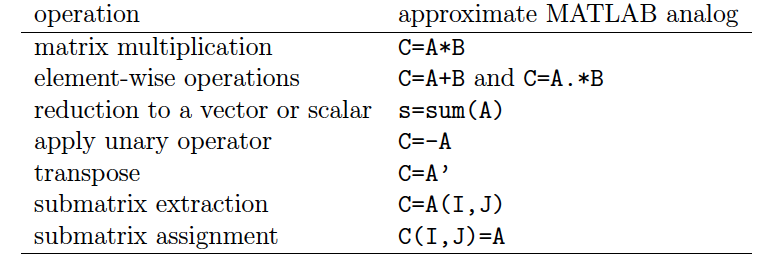
\includegraphics[width=0.8\textwidth]{figures/linear-algebra-apis.png}
\caption{A brief summary of linear algebra APIs.}
\label{fig:la-apis}
\end{figure}


\subsection{Merits of the linear algebra approach}

Expressing graph algorithm in the language of linear algebra is attractive, and the main advantages of the linear algebra approach is summarized as follows:
\begin{itemize}
  \item \textbf{conciseness:}
    By treating the graph as a sparse matrix, the core operations in many scalable graph algorithms can be presented by a small set of linear algebra operations, and these operations are parallelized by performance experts on various architectures.
    In this sense, the linear algebra approach is particularly preferable for distributed graph processing since it makes the communication completely transparent to the programmers.
    %There is a clear separation of concern for algorithm designer and performance expert, and any 

  \item \textbf{scalability:}
    The implementation of matrix and vector operations on distributed-memory can make use of both MPI and OpenMP to maximize its scalability, and a recent work~\cite{lacc} using the Combinatorial BLAS~\cite{combblas} library successfully solves the connected component problem on a graph with more than 50B edges, using a Cray XC40 supercomputer with 4K nodes ($262K$ cores).

  \item \textbf{portability:}
    Recently, GraphBLAS~\cite{graphblas} defines a standard set of linear-algebraic operations for implementing graph algorithms, which makes it much easier for programmers to transform a linear algebra graph computation from one platform to another.

\end{itemize}


    %Several independent systems have merged that use matrix algebra to perform graph computations~\cite{combblas,gpi,graphpad,graphmat,yang2019graphblast}.

\begin{comment}
\subsection{Linear algebra APIs}


The following set of linear algebra operations are used in our description of graph algorithms.
%All the simplified APIs introduced below can be easily transformed to the GraphBLAS API.
%For readers who are interested, we provide full GraphBLAS implementations of our algorithms in the LAGraph library\footnote{\url{https://github.com/GraphBLAS/LAGraph}} for educational purpose.
\begin{itemize}
\item $\text{mxv}(\mathit{y}, \mathbf{A}, \mathit{x}, \otimes, \oplus)$: the sparse matrix-vector multiplication with user-specified binary operators $\otimes$ and $\oplus$.
%and the identity element $e$ for addition ($e\oplus a = a \oplus e = a$).
The output vector $y=\mathbf{A} x$ is computed by $y[i] = y[i] \oplus (a_{i,j} \otimes x[j])$ for $(i,j)\in \mathbf{A}$.
\item $\text{assign}(\mathit{y}, \mathit{mask}, \mathit{index}, \mathit{x}, \otimes)$: subvector assign with a user-specified binary operator $\otimes$.
The output vector $y$ is computed by $y[index[i]] = y[index[i]] \otimes x[i]$ for $i\in [0..n-1]$.
\item $\text{extract}(\mathit{y}, \mathit{mask}, \mathit{index}, \mathit{x})$: subvector extract, the dual operation of assign where $y[i] = x[index[i]]$ for $i\in [0..n-1]$.
\item $\text{eWiseMult}(\mathit{z}, \mathit{mask}, \mathit{x}, \mathit{y}, \otimes)$: generalized element-wise multiplication where $z[i] = x[i] \otimes y[i]$ for $i\in [0..n-1]$.
\item $\text{apply}(\mathit{y}, \mathit{mask}, \mathit{x}, f)$: apply the function $f$ to the entries of vector $x$ and store the results in vector $y$.
\item $\text{fill}(\mathit{x}, \textit{a})$: fill the vector $x$ with a scalar $a$.
\item $\text{copy}(\mathit{y}, \mathit{mask}, \mathit{x})$: copy the contents from vector $x$ to vector $y$.
\item $\text{select}(\mathbf{B},\mathbf{A},\text{selectOp})$: select a submatrix of $\mathbf{A}$ by a predicate function \text{selectOp} and store the result in $\mathbf{B}$.
\item $\text{reduce}(\textit{a}, \mathit{mask}, \mathit{x}, \oplus, \textit{e})$: reduce the elements in the vector $x$ to a scalar $a$ using a binary operator $\oplus$ and the identity $e$.
%\item $\text{build}(\mathbf{A}, \mathit{mask}, \mathit{i}, \mathit{j}, \mathit{x})$: construct a matrix $\mathbf{A}$ using the vectors $i$, $j$, $x$ for row indices, column indices and matrix elements.
\item $\text{getNVals} (\text{nvals}, \mathbf{A})$: get the number of elements in $\mathbf{A}$.
\item $\text{fillWithIndex} (\mathit{x})$: $x[i]=i$ for $i\in [0..n-1]$.
\end{itemize}
The $\mathit{mask}$ appeared in these functions is a boolean vector indicating the entries in the output vector that are to be modified.
Then, we denote \emph{zip} as a generic function that combines two tuples of any type into a larger tuple, in order to make our presentation clear.
\end{comment}

%\subsection{Problems of the linear algebra approach}

%Despite the conciseness, scalability and portability, the linear algebra approach however faces two problems
%\todo{todo}

\chapter{A custom Pregel system with optimizations as plug-ins}
\label{chap:vcgp}

Pregel's vertex-centric paradigm is widely adopted in many graph analytics systems, but as mentioned in the previous chapter, this model suffers performance issues when dealing with graph algorithms with complex communication patterns (e.g. the connected component algorithm and the minimum spanning forest algorithm) since Pregel's monolithic message mechanism cannot make use of multiple optimizations at the same time.

\begin{comment}
Such a vertex-program is an overloaded member function named \texttt{compute()} in a derived class of \texttt{Vertex}, whose template arguments decide the vertex type, edge type and message type of the graph application.
Messages from the previous superstep are available to the \texttt{compute()} method.
Besides, the base class \texttt{Vertex} also provides a set of auxiliary methods for \texttt{compute()}, like \texttt{send\_message()} for direct message passing and \texttt{vote\_to\_halt()} for deactivating itself.
The workers finally carries out the computation.
Each worker loads a portion of the graph and sets the vertices as active at the beginning.
Then, the graph computation is a series of BSP supersteps, and in each superstep the workers execute the user-specified \texttt{compute()} method on every active local vertex and exchange messages with each other.
In addition to the \texttt{compute()} function, users sometimes need to implement a specialized aggregator or combiner in a separate class.

\begin{figure}[t]
\begin{lstlisting}[basicstyle=\scriptsize\ttfamily,language=c++,morekeywords={override},
numbers=left,stepnumber=1,xleftmargin=2.5em,commentstyle=\color{xgreen}]
// the user-specified vertex value
struct PRValue {
   double PageRank;
   vector<int> Edges;
};
// the main class for the computation logic
class PageRankVertex : public
      Vertex<int, PRValue, double> {
public:
   void compute(MessageContainer &msgs) override {
      if (step_num() == 1) {
         value().PageRank = 1.0 / get_vnum();
      } else {
         double sum = 0;
         for (auto msg : messages)
            sum += msg;
         // s: the pagerank of the "sink node"
         double s = *(double*) getAgg() / get_vnum();
         value().PageRank = 0.15 / get_vnum()
              + 0.85 * (sum + s);
      }
      if (step_num() < 31) {
         int numEdges = value().Edges.size();
         if (numEdges > 0) {
            double msg = value().PageRank / numEdges;
            for (auto e : value().Edges)
             send_message(e, msg);
         }
      } else
         vote_to_halt();
   }
};
\end{lstlisting}
\caption{PageRank implementation in Pregel+.}
\label{fig:pagerank-pregel}
\end{figure}
\end{comment}

In this chapter, we propose a new approach to composing various optimizations together, by making use of the interface called {\em channel}~\cite{husky} as a replacement of Pregel's message passing mechanism.
Informally, a \text{channel} is responsible for sending or receiving messages of a certain pattern for some purpose (such as reading all neighbors' states, requesting data from some other vertex and so on).
And by slicing the messages by their purpose and organizing them in channels, we can characterize each channel by high-level communication patterns, identify the redundancies or potential performance issues, and then provide separate implementations to deal with their own issues.

The technical contributions of this work can be summarized as follows.
\begin{itemize}
\item First, we provide Pregel with a channel-based vertex-centric programming interface, which is intuitive in the sense that it is just a natural extension of Pregel's monolithic message mechanism.
%We show, through several examples, that it is convenient to optimize a Pregel program by simply using a proper channel from the channel library.
%also provide three optimized channels as a library, so that whenever applicable, users can easily optimize a program by simply replacing a message passing channel by an optimized one.
To demonstrate the power of the channel interface, we implement three optimizations as special channels and show how they are easily composed to optimize complex algorithms such as the above SV algorithm.

%\item Second, we provide a systematic mechanism for users to add new channels for new optimizations with modest effort, making the channel construction be highly modular.
%We present the design of our channel mechanism, and demonstrate how three interesting channels can be implemented for capturing three types of optimizations on our system.

\item Second, we have fully implemented the system and the experiment results convincingly show the usefulness of our approach.
The channel interface itself contributes to an up to $76\%$ reduction of message size especially for complex algorithms, and the three optimized channels further improve the performance of the algorithms they are applicable (3.50x for PageRank, 4.41x for Pointer-Jumping and 5.20x for weakly connected components).
%, and outperform the state-of-the-art Pregel systems.
% with the extensions of request-respond paradigm, mirroring technique and block-centric computation.
Specially, the composition of different optimizations makes the SV algorithm 3.39x faster than the best implementation available now.
\end{itemize}

\begin{comment}
%When programming in Pregel, users write a \textit{vertex-program} to implement a graph algorithm.
As a concrete example that will be used for comparison later,
\autoref{fig:pagerank-pregel} shows the implementation of PageRank~\cite{google,pregel} in a typical open-source version of Pregel called \PP{}~\cite{yan2015effective}.
%In this implementation, the \texttt{PageRankVertex} class inherits from \texttt{Vertex}, and users have to override the \texttt{compute()} function to implement the algorithm logic.
%The \texttt{PageRank} value of each vertex is initialized as \texttt{1/get\_vnum()} in the first superstep (line 12).
The \texttt{PageRank} value is initialized at the beginning (line 13).
In the first 30 supersteps, each vertex sends along outgoing edges (if exists) its tentative PageRank divided by the number of outgoing edges (lines 23--25).
Starting from superstep 2, each vertex gets the sum of the values arriving on messages, and calculate a new PageRank (lines 14--20).
To avoid PageRank lost in dead ends, conceptually we connect the vertices without outgoing neighbors to a virtual \textit{sink} node, and this sink node further connects to every vertex in the graph indicating a random jump with even distribution.
%Therefore, users implement an aggregator which collects the sum of PageRank from those vertices, and in the \texttt{compute()} function we include this value in the PageRank calculation (line 18).
To avoid PageRank lost in dead ends (vertices without outgoing edges), programmers use an aggregator to collect the sum of PageRank from them and give it back to all vertices in the next superstep (line 16--18).
Finally, every vertex invokes \texttt{vote\_to\_halt()} in superstep 31 (line 29), so the computation terminates before the next superstep since no messages are sent.
\end{comment}

\begin{table}[t]
\centering
\caption{The APIs for standard channels.}
\label{tab:basic-apis}
\resizebox{\columnwidth}{!}{
\begin{tabular}{l|l|l}
\hline
  \multicolumn{2}{c|}{\textbf{Message-Passing Channels}}
& \textbf{Aggregator Channel} \\
\hline
% constructor
  \inlineCPP{DirectMessage(Worker<VertexT> *w);}
& \inlineCPP{CombinedMessage(Worker<VertexT> *w,}
& \inlineCPP{Aggregator(Worker<VertexT> *w,} \\

& \inlineCPP{\ \ \ \ Combiner<ValT> c);}
& \inlineCPP{\ \ \ \ Combiner<ValT> c);} \\
\hline
% main APIs
  \inlineCPP{void send_message(KeyT dst, ValT m);}
& \inlineCPP{void send_message(KeyT dst, ValT m);}
& \inlineCPP{void add(ValT v);} \\
  \inlineCPP{MsgIterator<KeyT, ValT> \&get_iterator();}
& \inlineCPP{const ValT \&get_message();}
& \inlineCPP{const ValT \&result();} \\
\hline
\end{tabular}
}
\end{table}

\begin{table}[t]
\centering
\caption{The APIs for special channels targeting specific communication patterns.}
\label{tab:apis}
\resizebox{\columnwidth}{!}{
\begin{tabular}{l|l|l}
\hline
  \textbf{Scatter-Combine}
& \textbf{Request-Respond}
& \textbf{Propagation (Simplified)} \\
\hline
% constructor
  \inlineCPP{ScatterCombine(Worker<VertexT> *w,}
& \inlineCPP{RequestRespond(Worker<VertexT> *w,}
& \inlineCPP{Propagation(Worker<VertexT> *w,} \\
  \inlineCPP{\ \ \ \ Combiner<ValT> c);}
& \inlineCPP{\ \ \ \ function<RespT(VertexT)> f);}
& \inlineCPP{\ \ \ \ Combiner<ValT> c);} \\
\hline
% initialization
  \inlineCPP{void add_edge(KeyT dst);}
&
& \inlineCPP{void add_edge(KeyT dst);} \\
\hline
% main APIs
  \inlineCPP{void set_message(ValT m);}
& \inlineCPP{void add_request(KeyT dst);}
& \inlineCPP{void set_value(ValT m);} \\
  \inlineCPP{const ValT \&get_message();}
& \inlineCPP{const RespT \&get_response();}
& \inlineCPP{const ValT \&get_value();} \\
\hline
\end{tabular}
}
\end{table}

\section{Programming with channels}
\label{sec:programming}

The channel mechanism is designed to help users organize the communications in vertex-centric graph algorithms.
Concretely speaking, the channels are message containers equipped with a set of methods for sending/receiving messages or supporting a specific communication pattern (see \autoref{tab:basic-apis} and \autoref{tab:apis} for the standard and optimized channels; the details are in \autoref{sec:opt-channels}).
In this section, we first introduce the programming interface using the PageRank example, then we show how different optimizations can be easily composed via channels in a more complex algorithm called the SV~\cite{ShVi82}.

\subsection{A standard PageRank implementation using channels}

Writing a vertex-centric algorithm in our system using the standard channels is rather straightforward for a Pregel programmer.
We present a PageRank Implementation in \autoref{fig:pagerank-channel}, which is basically obtained from a Pregel program (a vertex-centric \texttt{compute()} function with a parameter of received messages from the previous superstep) by replacing the sending/reading of messages by one or more user-defined message channel's send/receive methods.

In the first 30 supersteps, each vertex sends along outgoing edges (if exists) its tentative PageRank divided by the number of outgoing edges (lines 21--25), over a user-defined message channel \texttt{nbr}.
This channel is an instance of \texttt{CombinedMessage}, which requires a combiner to be provided in its constructor (line 9).
In the next superstep, every vertex gets the sum of the message values arriving on this channel (lines 18) and calculates a new PageRank.
%To obtain this implementation, users just need to allocate the channels and replace the matched send/receive pairs in the Pregel program with the same (message passing) channel's send/receive methods.
To avoid PageRank lost in dead ends (vertices without outgoing edges), we need a \textit{sink} node to collect the PageRank from those dead ends and redistribute it to all nodes, which is implemented by an aggregator \texttt{agg} using the addition operator (line 9).
Then, in line 27, users explicitly add the PageRank of the dead ends to the aggregator, and in the next superstep the sum is returned by the aggregator's \texttt{result()} method (line 16).
%Therefore, users implement an aggregator which collects the sum of PageRank from those vertices, and in the \texttt{compute()} function we include this value in the PageRank calculation (line 18).

\begin{comment}
A minor difference is that, this function is no longer a member function of \texttt{Vertex}, and the current vertex's state is accessed through the parameter.
For clear presentation, we use a micro \texttt{value()} to refer to the current vertex's value.
The \texttt{compute()} function is overall similar to the Pregel version shown in \autoref{fig:pagerank-pregel}, which contains the initialization (line 14), message sending (lines 21--27), message reading (lines 16--18) and termination (line 29).

In our system, there is no longer a message list or a global \texttt{send\_message()} function provided in the \texttt{compute()} function, and the functionality of message passing is provided by the user-defined channels.
To do so, a message passing channel \texttt{ch1} is defined at line 9, where the message type is specified as \texttt{double}.
\end{comment}

\begin{figure}[t]
\begin{lstlisting}[basicstyle=\scriptsize\ttfamily,language=c++,morekeywords={override},
numbers=left,stepnumber=1,xleftmargin=2.5em,commentstyle=\color{xgreen}]
using VertexT = Vertex<int, PRValue>;
auto c = make_combiner(c_sum, 0.0); // a combiner
class PageRankWorker : public Worker<VertexT> {
private:
   // two channels are defined here
   CombinedMessage<VertexT, double> nbr;
   Aggregator<VertexT, double> agg;
public:
   PageRankWorker():nbr(this, c), agg(this, c) {}

   void compute(VertexT &v) override {
      if (step_num() == 1) {
         value().PageRank = 1.0 / get_vnum();
      } else {
         // s: the pagerank of the "sink node"
         double s = agg.result() / get_vnum();
         value().PageRank = 0.15 / get_vnum()
               + 0.85 * (nbr.get_message() + s);
      }
      if (step_num() < 31) {
         int numEdges = value().Edges.size();
         if (numEdges > 0) {
            double msg = value().PageRank / numEdges;
            for (int e : value().Edges)
               nbr.send_message(e, msg);
         } else
            agg.add(value().PageRank);
      } else
         vote_to_halt();
   }
};
\end{lstlisting}
\caption{PageRank implementation using channels.}
\label{fig:pagerank-channel}
\end{figure}

\begin{comment}
The \texttt{msg} is the user-defined channel.
Whenever sending or receiving messages, we attach the channel name \texttt{msg} before the send/receive functions to distinguish it with the other communication channels.
The \texttt{msg} channel is an instance of \texttt{CombinedMessage}, which requires a user-specified combiner in its constructor (line 9).

The computation is implemented in a user-defined \texttt{compute()} function (line 11).
The message list in \autoref{fig:pagerank-pregel} is disappeared, whose replacement is a user-defined channel \texttt{msg}.
The class name \texttt{CombinedMessage} (line 6) indicates that this channel uses a combiner for message reduction, and it is at line 9 that the channel is initialized by a user-provided combiner \texttt{c}.
In the \texttt{compute()} function we can clearly see that when sending messages (line 24), we need to specify which channel we send the messages to, so the channel name \texttt{msg} is attached before the \texttt{send\_message()}.
Similarly, we read the combined message by invoking \texttt{msg}'s \texttt{get\_message()} method.
When no message is to be received, a vertex simply sees a zero (the identity value of the combiner), which will not affect the correctness of the algorithm.

Then, \texttt{agg} (defined at line 7) is another channel which plays the role of an aggregator in the PageRank implementation.
It stores a global value, and all vertices can access it via the \texttt{result()} method (line 16).
Slightly differ from Pregel+, users explicitly add a vertex's PageRank value to the aggregator (line 27), and the operator is given in the constructor of \texttt{agg}.
%The combiner provided in the constructor of \texttt{agg} indicates that we are expected to see the sum of all values added to \texttt{agg} in the previous superstep.
\end{comment}

All the computation logic and the channels are written in a user-defined class called \texttt{PageRankWorker} that inherits from the \texttt{Worker} class in our system.
The type of vertex ID and value type are packed in to the \texttt{VertexT} type and provided to the \texttt{Worker} class.
We leave the explanation of \texttt{Worker} in the next section, and users just keep in mind that programs in our system are constructed in this way.

\subsection{Channels and optimizations}

In our channel-based system, we offer a set of optimizations as special channels (in \autoref{tab:apis}), which can be regarded as more efficient implementations (compared to the standard message passing channels) of several communication patterns.
Here, we demonstrate how to enable the scatter-combine optimization (which deals with the ``static messaging pattern'') for PageRank.
The details of this optimization will be presented in \autoref{sec:opt-channels}.

Given a channel-based PageRank implementation in \autoref{fig:pagerank-channel}, 
what we need to do is simply switching the standard message channel \texttt{msg} to the scatter-combine channel.
First, we change the definition of \texttt{nbr} as follows:
\begin{lstlisting}[style=highlight,firstnumber=5]
   // change to the scatter-combine channel
   @ScatterCombine@<VertexT, double> nbr;
\end{lstlisting}
Then, in the \texttt{compute()} function, we initialize the scatter-combine channel (by invoking the \texttt{add\_edge()} method) before actually sending any data, which is done in the first superstep as below:
\begin{lstlisting}[style=highlight,firstnumber=12]
   if (step_num() == 1) {
      value().PageRank = 1.0 / get_vnum();
      // provide the graph topology to the channel
      @for (int e : value().Edges)@
         @nbr.add_edge(e);@
   } ...
\end{lstlisting}
Finally, we switch to the scatter-channel's dedicated interface for message passing, which is \texttt{set\_message()} indicating a unique message value for all neighbors:
\begin{lstlisting}[style=highlight,firstnumber=22]
   if (numEdges > 0) {
      double msg = value().PageRank / numEdges;
      // no need to specify the destination
      @nbr.set_message(msg);@
   } ...
\end{lstlisting}
The rest of the program remains the same.
Our experiments (\autoref{sec:eval-sc}) show that, by switching to the scatter-combine channel, the PageRank immediately gets 3x faster, and all the programmer need to understand is the high-level abstraction of each channel.
%In the next section, we will use a more complex example to show that such design is necessary.

\begin{comment}
In our channel-based system, we offer a set of optimizations, and each of them can be regarded as a more efficient implementation (compared to the message passing channels) for a particular communication pattern.
In this part, we focus on how users can use them to optimize a program, while the ideas and implementations of these optimizations are presented in \autoref{sec:opt-channels}.

First of all, the optimizations in our system are provided as specially implemented channels, each of which may have different assumptions and provides its own interface to interact with vertices.
\autoref{tab:apis} summarizes the interfaces of our optimized channels.
Here we look at the scatter-combine channel in the middle column, which will soon appear in our PageRank example.
This optimization assumes that in each superstep, each vertex always sends the same message value to all of its outgoing neighbors, and the receiver only needs a combined message value.

The scatter-combine channel works in the following way.
First, it requires each vertex to provide its neighbors by invoking the \texttt{add\_edge()} method,
so that the graph topology is available to the channel.
Then, it asks every vertex to provide a single message value, and the channel will automatically dispatch it to all neighbors according to the graph topology.
A combiner is required in the constructor, so in the next superstep, the receiver gets the combined message value by \texttt{get\_message()}.
We present the improved version of PageRank using this channel in \autoref{fig:pagerank-scatter}, where the changes are highlighted in the program.

\begin{figure}[t]
\begin{lstlisting}[style=highlight]
using VertexT = Vertex<int, PRValue>;
class PageRankWorker : public Worker<VertexT> {
private:
   // change to a scatter-combine channel
   @ScatterCombine<VertexT, double> ch1;@
   Aggregator<VertexT, double> ch2;
public:
   PageRankWorker():
         ch1(this, make_combiner(c_sum, 0.0)),
         ch2(this, make_combiner(c_sum, 0.0)) {}

   void compute(VertexT &v) override {
      if (step_num() == 1) {
         value().PageRank = 1.0 / get_vnum();
         // provide graph topology to the channel
         @for (int e : value().Edges)@
            @ch1.add_edge(e);@
      } else {
         double s = ch2.result() / get_vnum();
         value().PageRank = 0.15 / get_vnum()
               + 0.85 * (ch1.get_message() + s);
      }
      if (step_num() < 31) {
         int numEdges = value().Edges.size();
         if (numEdges > 0) {
            double msg = value().PageRank / numEdges;
            // no need to specify the destination
            @ch1.send_message(msg);@
         } else
            ch2.add(value().PageRank);
      } else
         vote_to_halt();
   }
};
\end{lstlisting}
\caption{An improved version of PageRank using the scatter-combine channel.}
\label{fig:pagerank-scatter}
\end{figure}

In the channel definition, the channel name is changed to \texttt{ScatterCombine} while the template arguments remain the same.
At the first superstep, users provide the graph topology to \texttt{ch1} by making each vertex add the outgoing neighbors through the \texttt{add\_edge()} function (lines 24--25).
%The message passing interface for the scatter-combine channel is slightly different.
A vertex provides a single message value to the channel (line 36), then the channel will propagate that message according to the graph topology.
%The interface itself indicates that a vertex always provides the same message value to all its neighbors in each superstep.
Our experiments show that, by switching to the scatter-combine channel, the PageRank runs 2x--5x faster than the ordinary version.
\end{comment}

\subsection{Composition of channels}
\label{sec:sv-algo}

%When building complicated algorithms, our channel-based system allows users to allocate different types of channels to handle multiple performance issues in the same program.

In this part, we use a more complicated example called the Shiloach-Vishkin (SV) algorithm~\cite{ShVi82} to show that,
users can easily combine different optimizations (channels) to handle multiple performance issues in the same program.
%To clearly see the performance issues and to better understand the experiment results, we will first present the high-level description of this algorithm and then discuss how the channels are chosen according to the communication pattern in this algorithm.
%Finally, we sketch an implementation for interested readers.

\subsubsection{The SV Algorithm}

%The SV algorithm is designed for efficiently finding the connected components in undirected graphs with large diameters (e.g., road network), which is guaranteed to terminated in $O(\log n)$ supersteps where $n$ is the number of vertices in the graph.

The SV algorithm is in general an adaptation of the classic union-find algorithm~\cite{disjointset} to the distributed setting, which finds the connected components in undirected graphs with $n$ vertices in $O(\log n)$ supersteps.
In the SV algorithm, the connectivity information is maintained by a distributed tree structure called disjoint-set~\cite{disjointset}, where each vertex holds a pointer which points to either some other vertex in the same connected component or to itself.
We henceforth use $D[u]$ to represent this pointer for vertex $u$.
Following is the high-level description of the SV algorithm using a domain-specific language called Palgol~\cite{palgol}, and it compiles to Pregel+ code\footnote{The Palgol code is presented here for easy understanding. It currently compiles to Pregel+ using only the message interface, and the the performance is close to the hand-written code~\cite{palgol}.}.

\begin{comment}
Specifically, the data structure is a forest, and vertices in the same tree are regarded as belonging to the same connected component.
Each vertex maintains a parent pointer that either points to some other vertex in the same connected component, or points to itself, in which case the vertex is the root of a tree.
We henceforth use $D[u]$ to represent this pointer for each vertex $u$.
Following is the high-level description of the SV algorithm using a domain-specific language called Palgol~\cite{palgol}, which basically makes the vertices globally accessible to ease Pregel programming.
\end{comment}

\begin{lstlisting}[basicstyle=\scriptsize\ttfamily,language=palgol,
numbers=left,stepnumber=1,xleftmargin=2.5em,commentstyle=\color{xgreen},numberfirstline=false]
// initially suppose we have D[u] = u for every u
do
  // enter vertex-centric mode
  for u in V
    // whether u's parent is a root vertex
    if (D[D[u]] == D[u])
      // iterate over neighbors (D[e]: neighbor's pointer)
      let t = minimum [ D[e] | e <- Nbr[u] ]
      if (t < D[u])
        // modify the D field of u's parent D[u]
        remote D[D[u]] <?= t
    else
      // the pointer jumping (path compression)
      D[u] := D[D[u]]
  end
until fix[D] // until D stabilizes for every u
\end{lstlisting}

Starting from $n$ root nodes, the SV algorithm iteratively merges the trees together if crossing edges are detected.
In a vertex-centric way, every vertex~$u$ simultaneously performs one of the following operations depending on whether its parent $D[u]$ is a root vertex:
\begin{itemize}
 \item \textbf{Tree merging (lines 7--11).}
  If $D[u]$ is a root vertex, $u$ sends the smallest one of its neighbors' pointer (to which we give a name $t$) to the root $D[u]$ and later the root points to the minimum $t$ it receives (to guarantee the correctness of the algorithm).
 \item \textbf{Pointer jumping (line 14).}
  If $D[u]$ is not a root vertex, $u$ modifies its pointer to its ``grandfather'' ($D[u]$'s current pointer).
  Since all the vertices below the children of root perform this operation simultaneously, it halves the distance to the current root.
\end{itemize}
The algorithm terminates when all vertices' pointers do not change after an iteration.
Readers interested in the correctness of this algorithm can be found in the original paper~\cite{yan2015effective} for more details.

\begin{comment}
\begin{itemize}
 \item \textbf{Tree merging (lines 9--13).}
  if $D[u]$ is a root vertex, then $u$ chooses one of its neighbors' current parent (to which we give a name $t$), and makes $D[u]$ point to $t$ if $t<D[u]$ (to guarantee the correctness of the algorithm).
  When having multiple choices in choosing the neighbors' parent $p$, or when different vertices try to modify the same parent vertex's pointer, the algorithm always uses the ``minimum'' as the tiebreaker for fast convergence.
 \item \textbf{Pointer jumping (line 15).}
  if $D[u]$ is not a root vertex, then $u$ modifies its own pointer to its current ``grandfather'' ($D[u]$'s current pointer).
  This operation halves $u$'s distance to the root vertex, and will eventually make~$u$ a direct child of the root vertex so that it can perform the above tree merging operation.
\end{itemize}
The algorithm terminates when all vertices' pointers do not change after an iteration, in which case all vertices point to some root vertex and no more tree merging can be performed.
Readers interested in the correctness of this algorithm can be found in the original paper~\cite{yan2015effective} for more details, and a baseline implementation can be obtained by compiling the Palgol code shown above.
\end{comment}

\subsubsection{Choices of Channels}

In the SV algorithm, three major performance issues are identified below by analyzing the communication patterns in the algorithm.
\begin{itemize}
 \item The load balance issue in testing whether $D[u]$ is a root vertex or not for every $u$.
  The standard implementation is to let each $u$ send a request to its current parent $D[u]$, then the reply message is the parent's pointer.
  Due to the pointer jumping, the height of the tree will decrease and the width of the tree will increase, causing a few vertices with very large degree to slow down the reply phase.
%  Due to the pointer jumping, the tree will become lower and wider, causing a few vertices having a large degree and thus taking a long time in the reply phase.
  %We use a technique called request-respond paradigm (see \autoref{sec:request-respond}) to solve the problem.
 \item The heavy neighborhood communication in calculating the minimum parent ID of the neighboring vertices, where all vertices need to send a unique message value to all neighbors, regardless of the vertices' local state.
  %Our scatter-combine channel with a combiner of minimum operation optimizes exact such scenario.
 \item The congestion issue in the modification of parent's pointer, due to the existence of high-degree vertices.
\end{itemize}

We provide the solutions to all of these issues in our system as special channels, and users just need to choose the proper channels and combine them together in the program.
%It is rather a design choice, because in practice, the choice of channels may depend on the algorithm, the input graph and probably other things.
For the SV algorithm,
the load balance issue can be avoided by the request-respond channel, the heavy neighborhood communication is optimized by the scatter-combine channel, and a message channel with combiner solves the congestion issue.

\begin{comment}
The implementation of SV needs four channels, where an additional aggregator is used to check whether all vertices have stabilized.
We sketch an implementation in \autoref{fig:sv-code}.
The main computation basically repeats the following four supersteps.
In superstep 1, every vertex sends a query to its parent vertex over a request-respond channel, and gets the grandparent ID from the parent vertex in superstep 2.
Moreover, every vertex sends its own parent ID to all neighbors in superstep 1 over a scatter-combine channel.
In superstep 2, each vertex gets all the necessary data, then it performs either tree merging or pointer jumping according to whether its parent is a root.
For the tree merging operation, a message is sent to the parent vertex over a combined-message channel, and that message is handled in superstep 3.
Next, all the vertices decide whether to stop the algorithm by combing their each decision via the aggregator.
Finally in superstep 4, they terminate the computation or start another iteration according the result of the aggregation.
\end{comment}

\section{Channel implementation}
\label{sec:opt-channels}

In this section, we present the design of our channel mechanism and demonstrate how three interesting channels are implemented for dealing with different performance issues.

\subsection{Overview}

\begin{figure}[t]
 \centering
 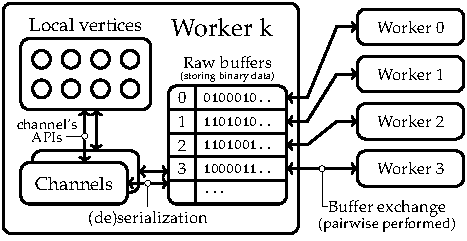
\includegraphics[width=0.75\textwidth]{figures/channel.pdf}
 \caption{The architecture of our channel-based system.}
 \label{fig:channels}
\end{figure}

\autoref{fig:channels} shows the architecture of our channel-based system.
Worker is the basic computing unit in our system.
%, where the terminology comes from the \PP{} \cite{yan2015effective}. Similar to \PP{},
When launching a graph processing task, multiple instances of workers are created, each holding a disjoint portion of the graph (a subset of vertices along with their states and adjacent lists).
Workers share no memory but can communicate with each other.
Such big picture is common in all Pregel systems, but ours has a unique hierarchy of the components inside the worker.

In our system, channels form an independent layer inside the worker between the vertices and the raw buffers.
Each worker has $M-1$ buffers (where $M$ is the number of workers launched by the user) for storing binary message data for each other worker,
then the channels can read or write its own address space on these buffers.
The system simply exchanges the contents of the buffers pairwise using the MPI in every superstep.
%A simple operation called \textit{buffer exchange} is to exchange the data pairwise using the MPI.
Each channel independently implements a communication pattern (like messages passing or aggregator) and exposes its own interfaces (like \texttt{send\_message(dst, msg) for a message channel}) to the vertex.
To implement an algorithm, users should inherit the \texttt{Worker} class, override the \texttt{compute()} function and allocate the channels that are suitable for the algorithm according to the communication patterns it has.

%and then users choose the proper channels to implement a graph algorithm according to the communication patterns it has.
%To implement an algorithm, users should inherit the \texttt{Worker} class, override the \texttt{compute()} function and choose proper channels according to the communication patterns in the algorithm.

\begin{comment}
At the bottom, each worker maintains $M-1$ buffers (where $M$ is the number of workers) for storing binary data (like messages) to every other, then a simple operation called \textit{buffer exchange} is to deliver all the data to the destinations, where the workers exchange the data pairwise using the MPI.

Upon this simple communication mechanism, standard or optimized channels are implemented as independent classes to support communication patterns that are well-known in vertex-centric model (like message passing or aggregator).
%In a word, the worker is the core of the system, while the channels are extended libraries.
To implement an algorithm, users should inherit the \texttt{Worker} class, override the \texttt{compute()} function and choose proper channels according to the communication patterns in the algorithm.
More details about the channels are introduced in the next section.
\end{comment}

\begin{figure}[t]
\begin{lstlisting}[basicstyle=\scriptsize\ttfamily,language=c++,morekeywords={override},
numbers=left,stepnumber=1,xleftmargin=2.5em,commentstyle=\color{xgreen}]
class Channel {
public:
   // initialization function
   virtual void initialize() {};
   // paired (de)serialization functions
   virtual void serialize(Buffer &buff) = 0;
   virtual void deserialize(Buffer &buff) = 0;
   // return true for additional buffer exchange
   virtual bool again() { return false; };
};
\end{lstlisting}
\caption{The core functions of the base class \texttt{Channel}.}
\label{fig:channel-class}
\end{figure}

\subsection{Design principle}
\label{sec:principle}

The channel mechanism mainly targets (but not limited to) a class of optimizations that handles the redundancies in communication.
For example, the standard combiner optimization~\cite{pregel} allows the worker to combine the messages sent to the same destination by a user-defined binary operator, and the request-respond paradigm~\cite{yan2015effective} merges the requests to the same destination to avoid sending redundant copies of the same value.
In these optimizations, typically, each worker processes all the messages in batch and sends a more compact but equally informative message list.
After the messages are delivered, the receiver worker may further process the data and dispatch the messages to the vertices.
%Then, it sends the result to the designated worker, while the receiver may further process the data.

Having such common pattern in these communication related optimizations, our channel mechanism tries to organize them in a modular way and make them work perfectly with the Pregel abstraction.
Essentially, each channel is a user-specified message handler that is invoked by the worker in every superstep.
The vertices actually put messages into (or fetch messages from) the channels' local storage through each channel's dedicated APIs, and the message handler can access all the local data of the channel as well as current worker's states to implement a particular communication pattern.
Channels are registered on the worker, so the composition of channels is actually trivial, which is accomplished by the worker carefully separating the messages of each channel in its message buffer.

%Our channel mechanism is designed for two purposes: providing a good separation for messages of different communication and optimization patterns, and allowing users to implement new optimizations as channels with ease.
%In other words, we are going for modularity and extensibility for optimizations.
%The first goal, modularity, is relatively easy to achieve by regarding each channel as a separate message buffer (on top of the worker's raw buffer) which stores only the messages it requires and applies a specific optimization.
%The second goal, extensibility, requires a more careful design of how the channel interacts with the worker.

\subsection{The channel interface}

\autoref{fig:channel-class} shows the base class \texttt{Channel} and its core functions: \texttt{initialize()}, \texttt{serialize()} for writing data to worker's raw buffer, \texttt{deserialize()} for reading data from worker's raw buffer (after the buffer exchange) and \texttt{again()} for supporting multiple rounds of communication.
All the channels in our paper are implemented as derived classes of \texttt{Channel} with proper implementations of these four functions (in particular \texttt{serialize()} and \texttt{deserialize()}).

To clearly see how the workers and channels cooperate with each other, we present the computation logic of the worker in \autoref{fig:channel-logic}.
The worker's computation is organized as synchronized supersteps.
In each superstep, the worker first calls the \texttt{compute()} on every vertex, then it performs several rounds of buffer exchanges.
In each round, the system invokes the active channels' \texttt{serialize()} and \texttt{deserialize()} methods to exchange the data between the channels and the buffers.
%The main functionality of channels is also implemented in the paired (de)serialization functions.
%collect from the channel the data to send, or let channels read the received data from the buffer.
All channels are set to active at the beginning, but they can deactivate themselves by returning \texttt{false} in the \texttt{again()} function.
Channels' \texttt{initialize()} is invoked at the beginning of the computation,
in which the channel can access the basic information of the graph (like graph size, number of vertices on the current worker) for initialization.
While not explicitly presented in the code, the channels can activate vertices through the \texttt{Worker}'s interface by providing the vertex's ID or local index.
That is how our system simulates the voting-to-halt mechanism of Pregel.

\begin{comment}
Let us just take the \texttt{CombinedMessage} channel as an example, which needs one buffer exchange to deliver all the messages (a pair of destination ID and message value) collected from the local vertices.
Its \texttt{serialize()} function sorts the messages by destination ID and merges the messages for the same vertex into a single message containing the combined message value, and after buffer exchange, the channel reads the messages from the buffer and dispatches them to the local vertices in the \texttt{deserialize()} function.
For this channel, \texttt{again()} always returns \texttt{false} and \texttt{initialize()} is empty.
\end{comment}

\begin{figure}[t]
\begin{lstlisting}[style=highlight,
morekeywords={foreach,end_for,end_while}]
load_graph()
foreach channel c do c.@initialize@()
foreach vertex v do v.set_active(true)
while (active vertex exists) // a superstep
   foreach active vertex v do this.compute(v)
   foreach channel c do c.set_active(true)
   while (active channel exists)
      foreach active channel c do c.@serialize@()
      buffer_exchange()
      foreach active channel c do
         c.@deserialize@()
         c.set_active(c.@again@())
      end_for
   end_while
end_while
dump_graph()
\end{lstlisting}
\caption{The computation logic of the worker for illustrating the channel mechanism.}
\label{fig:channel-logic}
\end{figure}

\subsection{Case studies}

As the last part of this section, we demonstrate how to implement three optimizations, which target three important performance issues in vertex-centric graph processing.
%They are scatter-combine channel for redundant communication, request-respond channel for imbalanced workload, and propagation channel for low convergence speed.

\subsubsection{Scatter-Combine Channel}
\label{sec:scatter-combine}

The scatter-combine abstraction is a common high-level pattern appeared in many single-phase algorithms such as PageRank, single-source shortest path (SSSP) and connected component (CC).
%It was initially introduced by Graphine~\cite{graphine} as a vertex-centric variant of the GAS model~\cite{powergraph}.
The communication in this model is captured by a \texttt{scatter()} function on each vertex to send a unique value to all neighbors, and a \texttt{combine()} function to combine the messages for each receiver.
We focus on a special case where \textit{every} vertex needs to send a value to all of its neighbors\footnote{\small In some algorithms like SSSP or WCC, only active vertices need to send messages, which is not the case we are targeting here.} regardless of its local state.
An iterative algorithm having such static messaging pattern will waste time repeating the same message dispatching procedure, while a proper preprocessing can greatly reduce the computation time as well as the message size.
%Then, our special implementation of this communication pattern can significantly accelerate the message processing and reduce the communication volume at the same time.

%In a conventional implementation like \texttt{CombinedMessage}, the sorting of such massive messages is expensive but necessary in every superstep.
%However, with the knowledge that every vertex will repeatedly send messages to all neighbors, we made the sorting a preprocessing step, so that in the consequent supersteps the channel just uses a linear scan to calculate all the combined messages.

\begin{figure}[t]
 \centering
 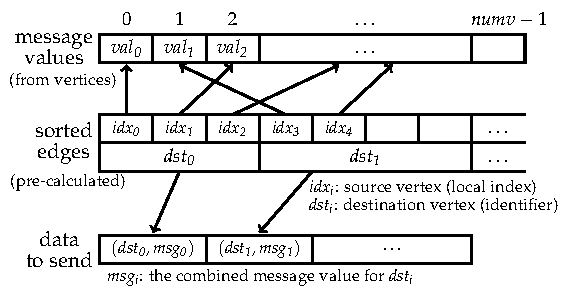
\includegraphics[width=0.8\textwidth]{figures/scatter-impl.pdf}
 \caption{The execution logic for the scatter-combine channel.}% Edges are sorted in advance. The combined message values can be obtained by scanning the array of sorted edges exactly once.}
 \label{fig:scatter-impl}
\end{figure}

\autoref{fig:scatter-impl} demonstrates the computation logic of the scatter-combine channel.
Suppose the vertices on an worker is indexed by \texttt{0..numv-1}, then each local edge is a pair $(idx, dst)$ where $idx$ refers to a local vertex and the $dst$ can be an arbitrary vertex in the graph.
We sort the edges by $dst$ in advance, then by scanning the array of the sorted edge list once, we can quickly calculate for each destination a combined message value.
This is much cheaper than the normal message routine which typically requires hashing or sorting.


%or communication-intensive algorithms such as PageRank, it can save a lot of time since the message processing dominates the execution time.

%In addition to the improvement on the execution time, we can further reduce the message size by avoiding redundant transmissions~\cite{lccgraph}.
%The key observation is that the $dst_i$ in the final list of combined messages will not change as long as the graph topology is the same.
%Therefore, the $dst_i$ are attached to the message value in the first round, and afterwards only the message values are transmitted.

The APIs for the scatter-combine channel are presented in the first column of \autoref{tab:apis}.
Users need to initialize the channel by adding the outgoing edges of each vertex through the \texttt{add\_edge()} function before the first message sending occurs in the execution.
Then, every vertex emits an initial messages using the \texttt{send\_message()} interface and the combined messages for each vertex can be obtained by the \texttt{get\_message()} method in the next superstep.

\subsubsection{Request-Respond Channel}
\label{sec:request-respond}

This is a communication pattern where two rounds of message passing (say the request phase and respond phase) together form a conversation to let every vertex request an attribute of another vertex.
Typically, such computation contains vertices with high degree which causes imbalanced workload in the respond phase, and the solution is to merge the requests of the same destination on each worker.
More details can be found in the original paper~\cite{yan2015effective}.

Our implementation of this optimization is illustrated in \autoref{fig:reqresp-impl}.
A request is a pair $(idx, dst)$ where $idx$ refers to a local requester and the $dst$ can be an arbitrary vertex in the graph.
The worker sorts the requests by $dst$ and sends exactly one message containing the worker ID to each of the unique destinations.
When receiving the response values, the worker performs another scan to the sorted requests, which is sufficient to reply to all the requesters.

\begin{comment}
The idea of the optimization is to merge the requests for the same destination on the same sending worker, so that each vertex only needs to handle at most one request from each worker, instead of individual requests from a potentially large number of vertices.
Therefore, this optimization avoids the bottleneck in communication and reduces the messages transferred in the network at the same time.
More details are referred to the original paper~\cite{yan2015effective}, and our implementation of this optimization is illustrated in \autoref{fig:reqresp-impl}.
\end{comment}

\begin{figure}[t]
 \centering
 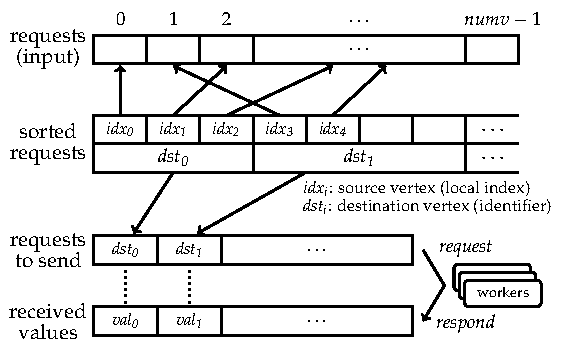
\includegraphics[width=0.8\textwidth]{figures/reqresp-impl.pdf}
 \caption{The execution logic for the request-respond channel.}% Requests are sorted and made unique. Two buffer exchanges then implement the request and respond phases. Received values are associated to the local vertices by another scan of the sorted requests.}
 \label{fig:reqresp-impl}
\end{figure}

The middle column of \autoref{tab:apis} shows the APIs of the request-respond channel.
When creating the channel, users need to provide a function that generates a response value from a vertex's state.
The whole procedure is implemented in an implicit style; A vertex invokes \texttt{add\_request()} with the destination vertex ID;
all the requests are delivered after the request phase, and the vertices receiving any request will be automatically involved, and a response value is produced by the user-provided function.


\begin{comment}
When initializing the channel, users need to provide a function which generates a response value from a vertex value.
In the \texttt{compute()} function, a vertex invokes \texttt{add\_request()} with the destination vertex ID.
The whole procedure is implemented in an implicit style; requests are delivered by the first buffer exchange, and the vertices receiving any request will be automatically involved, and a response value is generated by the user-provided function.
The response values are sent back to the requesting worker in the second buffer exchange and are dispatched to the requesting vertices by the channels.
In the next superstep, vertices who have ever sent a request in the previous superstep can fetch the result through the \texttt{get\_respond()} interface.
\end{comment}

\subsubsection{Propagation Channel}
\label{sec:propagation}

The last optimized channel is to speedup the convergence for a class of propagation-based algorithms.
In these algorithms, typically, some vertices emit the initial labels, and in each of the following supersteps, vertices receiving the labels will perform some computation and may further propagate a new label to their outgoing neighbors.
Since the propagation is between neighbors, such algorithms converge very slowly on graphs with large diameters.

The design of this channel is inspired by two existing techniques for improving the convergence speed.
First, the GAS model~\cite{powergraph} with an asynchronous execution mode can perform the crucial updates as early as possible without waiting for the global synchronization.
Although this implementation is not feasible in our synchronous system, the high-level abstraction is suitable for describing such kind of computation.
Second, the block-centric computation model~\cite{thinkgraph,yan2014blogel,goffish} is an extension of Pregel which opens the partition to users, so that users can choose a suitable partition method and implement a block-level computation to perform the label propagation within a connected subgraph.

Our propagation channel combines the advantages of these two techniques: it provides a simplified GAS model which naturally describes such propagation-based computation, and its implementation works in a similar way as a block-level program to accelerate the label propagation.
Therefore, users allocate a channel to obtain a performance gain without additional efforts on writing the block-level program.

\begin{figure}[t]
\centering
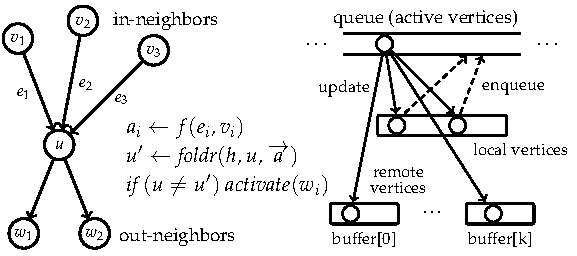
\includegraphics[width=0.8\textwidth]{figures/async-model.pdf}
\caption{The propagation channel's high-level model and computation logic.}
\label{fig:propagation-model}
\end{figure}

\autoref{fig:propagation-model} describes the high-level model for the propagation channel as well as the execution logic in our implementation.
Initially, each vertex is associated with a value and is set to active.
Whenever having an active vertex $u$ in the graph, it reads each incoming neighbors and the corresponding edges (if exists), and calculate a value $a_i$ by a user-provided function $f$.
Then, a combiner $h$ updates the original vertex value $u$ by each neighbor's $a_i$ and returns a new vertex value $u'$.
If the new value $u'$ is different from the original value $u$, we activate all outgoing neighbors of $u$ to propagate the update, and finally $u$ is deactivated after being processed.
The computation stops when all the vertices are inactive.
Note that we require $h$ to be commutative, so that the order of combining $a_i$ does not affect the result.
Moreover, when any of the incoming neighbors of $u$ is modified, $u$ needs to read the modified vertex to update its own value, instead of recomputing the $\mathit{foldr}$ by reading all its incoming neighbors' values.

This computation model is implemented by each worker performing a BFS-like traversal on the subgraph it holds.
Starting from the initial setting, each worker propagates the values along the edges as far as possible.
It updates the local vertices directly, but records the changes on remote vertices as messages.
The buffer exchange is performed after no update is viable on any worker.
After the remote updates triggered by messages, a new round of local propagation is performed.
It terminates when all vertices have converged.

The last column of \autoref{tab:apis} shows the APIs of a simplified propagation channel without considering the edge weights (for saving space), so users provide a combiner to calculate the new vertex value.
Each vertex adds its adjacent list to the channel via \texttt{add\_edge()} and sets the initial value by \texttt{set\_value()}, and in the next superstep, a vertex invokes \texttt{get\_value()} to get the final value after the propagation converges.
To make the best use of the propagation channel, users should properly partition the graph and attach the partition IDs to the vertex IDs.

\section{Evaluation}
\label{sec:vcgp-eval}

The experiments are conducted on an Amazon EC2 cluster of 16 nodes (with instance type m5.2xlarge), each having 8 vCPUs and 32G memory.
The connectivity between any pair of nodes in the cluster is 10Gb.
The datasets are listed in \autoref{tab:datasets} including both real-world graphs (Wikipedia\footnote{\small\url{http://konect.uni-koblenz.de/networks/dbpedia-link}}, Twitter\footnote{\small\url{http://konect.uni-koblenz.de/networks/twitter_mpi}} and SubDomain\footnote{\small\url{http://webdatacommons.org/hyperlinkgraph/2012-08/download.html}}) and synthesized graphs (Chain, Tree and RMAT~\cite{rmat}).
Graphs are converted to the required type (directed, undirected or weighted) for each algorithm in the experiments.

We select six representative algorithms in our evaluation, including PageRank (PR), Pointer-Jumping (PJ), Weakly Connected Component (WCC), SV algorithm (SV), Strongly Connected Component (SCC) and Minimum Spanning Forest (MSF).
For comparison, we also present the results of our best-effort implementations in \PP{} \cite{yan2015effective} and Blogel~\cite{yan2014blogel}.
Both of them are typical Pregel implementations, where \PP{} supports the request-respond paradigm and mirroring technique in two special modes (\textit{reqresp} mode and \textit{ghost} mode respectively) and Blogel supports the block-centric computation.
All of these systems mentioned above as well as our channel-based system are implemented in \CC{} on top of the Hadoop Distributed File System (HDFS).
The source code of our system can be accessed at \texttt{\url{https://bitbucket.org/zyz915/pregel-channel}}.

\begin{table}[t]
\centering
\caption{Datasets used in our evaluation}
\label{tab:datasets}
\begin{tabular}{c|c|c|c}
\hline
\textbf{Dataset} & $|V|$ & $|E|$ & avg. Deg \\
\hline\hline
SubDomain & 99.41M & 1.94B & 19.52 \\
\hline
Twitter & 41.65M & 1.47B & 70.51 \\
\hline
Tree$^{*}$ & 1.00B & 1.00B & 1.00 \\
\hline
Chain$^{*}$ & 1.00B & 1.00B & 1.00 \\
\hline
RMAT$^{*}$ &  400M & 2.00B & 5.00 \\
\hline
Wikipedia & 18.27M & 172.31M & 9.43 \\
\hline
%HostGraph$^{*}$ & \& weighted & 99.41M & 2.04B & 16.00 \\
\multicolumn{4}{c}{\hbox{datasets marked with $*$ are synthetic.}}
\end{tabular}
%\vspace{-8pt}
\end{table}

\subsection{Overhead of the channel mechanism}
\label{sec:eval-channel}

First, we evaluate the standard channels (the message passing channels and aggregator) in our system.
Basically, rewriting a Pregel program into a channel-based version is just about replacing the matched send-receive pairs into the same channel's send/receive function.
The message is chosen as small as possible, and we always use a combiner if applicable.
We compare both implementations to see whether there is any overhead or benefits introduced by our channel mechanism.

The experiment results are presented in \autoref{tab:eval-cmp}, where a straightforward rewriting achieves a speedup ranging from 1.16x to 4.16x among all the five algorithms on those datasets.
For SCC and SV, we also observe a significant reduction on message size ranging from $23\%$ to $62\%$.

\textbf{Analysis.}
The channel mechanism itself can improve the performance, due to the following two reasons.
First, our system allows users to specify a combiner to a channel whenever applicable, %since we can specify the combiner for each channel,
while in Pregel, we can specify a global combiner only when all the messages in the algorithm can use that combiner.
This difference makes our SV and SCC more message-efficient,
%For example, in SV, all the operations except the request-respond communication can be optimized by a combiner, so the combiner is disabled when using the basic mode of \PP{} (or any other Pregel-like systems).
%The combiner however plays a very important role in reducing the communication cost especially for dense graph like Twitter, and the ..
where the inapplicability of combiner in \PP{} causes a 4.16x and 2.10x message size for SV and SCC respectively on Twitter.

Second, our channel-based system allows users to choose different message types for different channels, while in \PP{}, a global message type is chosen to serve all communication in the program.
Then, the MSF (we refer to a particular version here~\cite{boruvka}) is a typical example that uses heterogeneous messages in different phases of the algorithm.
The largest message type is a 4-tuple of integer values for storing an edge, but the smallest one is just an \texttt{int}.

\begin{comment}
The channel interface does introduce some overhead, which causes our SCC implementation slightly worse than the one in Pregel+.
However, such overhead is only visible when the message synchronization dominates the execution time.
For SCC, it terminates in 1247 supersteps and in most supersteps the number of active vertices is extremely low (less than $0.01\%$).
\end{comment}

For the rest algorithms, there is no significant difference when implemented in two systems.
% their channel-based implementations are almost the same as the original Pregel version.
%We can see that the message size is exactly the same.
Still, our system reduces the runtime of PR and WCC by up to $26\%$ and $35\%$ (using the \texttt{CombinedMessage} class), and for PJ (using the \texttt{DirectMessage} class) the number is $52\%$.
We believe that the improvement is due to the choice of message interface (in particular the message iterator in \texttt{DirectMessage} instead of nested \CC{} vectors in \PP{}).
Nevertheless, we show that our system implementation is reasonably efficient.

\begin{table}[t]
\centering
\caption{Comparison of the basic implementation of graph algorithms in Pregel+ and channel-based system.}
\label{tab:eval-cmp}
%\resizebox{\columnwidth}{!}{
\begin{tabular}{c|c|c|c|c|c|c}
\hline
\multirow{2}{*}{PJ} & \multicolumn{2}{|c}{Chain} & \multicolumn{2}{|c|}{Tree} \\
\cline{2-7}
 & pregel & channel & pregel & channel \\
\hline
runtime (s) & 596.99 & 327.86 & 221.76 & 105.70 \\
\hline
msg (GB) & 463.86 & 463.86 & 89.17 & 89.17 \\
\hline
\hline
\multirow{2}{*}{SV} & \multicolumn{2}{|c}{RMAT} & \multicolumn{2}{|c}{SubDomain} & \multicolumn{2}{|c}{Twitter} \\
\cline{2-7}
 & pregel & channel & pregel & channel & pregel & channel \\
\hline
runtime (s) & 465.98 & 232.91 & 411.67 & 155.36 & 143.03 & 59.71 \\
\hline
msg (GB) & 212.64 & 112.49 & 298.62 & 71.82 & 115.96 & 28.53 \\
\hline
\hline
\multirow{2}{*}{PR} & \multicolumn{2}{|c}{RMAT} & \multicolumn{2}{|c}{SubDomain} & \multicolumn{2}{|c}{Twitter} \\
\cline{2-7}
 & pregel & channel & pregel & channel & pregel & channel \\
\hline
runtime (s) & 509.93 & 417.70 & 308.83 & 236.36 & 235.37 & 194.00 \\
\hline
msg (GB) & 413.03 & 413.03 & 160.99 & 160.99 & 128.81 & 128.81 \\
\hline
\hline
\multirow{2}{*}{WCC} & \multicolumn{2}{|c}{RMAT} & \multicolumn{2}{|c}{SubDomain} & \multicolumn{2}{|c}{Twitter} \\
\cline{2-7}
 & pregel & channel & pregel & channel & pregel & channel \\
\hline
runtime (s) & 65.36 & 42.31 & 54.61 & 41.02 & 22.58 & 17.47 \\
\hline
msg (GB) & 37.83 & 37.83 & 19.65 & 19.65 & 9.26 & 9.26 \\
\hline
\hline
\multirow{2}{*}{SCC} & \multicolumn{2}{|c}{RMAT} & \multicolumn{2}{|c}{SubDomain} & \multicolumn{2}{|c}{Twitter} \\
\cline{2-7}
 & pregel & channel & pregel & channel & pregel & channel \\
\hline
runtime (s) & 266.52 & 116.24 & 345.38 & 382.68 & 99.99 & 56.64 \\
\hline
msg (GB) & 118.56 & 91.09 & 132.07 & 62.99 & 77.53 & 45.79 \\
\hline
\hline
\multirow{2}{*}{MSF} & \multicolumn{2}{|c}{RMAT} & \multicolumn{2}{|c}{SubDomain} & \multicolumn{2}{|c}{Twitter} \\
\cline{2-7}
 & pregel & channel & pregel & channel & pregel & channel \\
\hline
runtime (s) & 547.98 & 319.86 & 200.07 & 138.71 & 138.92 & 119.27 \\
\hline
msg (GB) & 438.41 & 400.11 & 173.18 & 161.53 & 123.36 & 117.50 \\
\hline
\end{tabular}
\end{table}

\subsection{Effectiveness of optimized channels}

Here, we evaluate the efficiency of our optimized channels against the message passing channels using the applications that each kind of channel is applicable.
In this part, we choose rather simple algorithms, so that we can clearly see how optimized channels can improve the performance in different scenarios.

\subsubsection{Scatter-combine channel}
\label{sec:eval-sc}


%We evaluate the scatter-combine channel using the PageRank.
%by showing the results of three implementations presented in this thesis, which are the ordinary implementation in \PP{} and two channel versions using the \texttt{CombinedMessage} channel and the \texttt{ScatterCombine} channel respectively.
%Moreover, one implementation using \PP{}'s ghost mode (a.k.a. the mirroring technique~\cite{yan2015effective}) for message reduction is also evaluated, and the mirroring threshold is set to 16 in all cases.

\begin{comment}
\begin{figure}[t]
\includegraphics[width=\textwidth]{figures/pagerank.pdf}
\caption{Execution time (left) and message size (right) for PageRank on Wikipedia and LJ-DG.}
\label{fig:pagerank-result}
\end{figure}
\end{comment}

PageRank is a typical graph algorithm that can be optimized by the scatter-combine channel.
We test \PP{}'s basic implementation, \PP{}'s \textit{ghost} mode (a.k.a. the mirroring technique~\cite{yan2015effective}), the standard channel version (\autoref{fig:pagerank-channel}) and the scatter-combine channel version.
For \PP{}'s mirroring technique, we set the threshold to 16 in all cases.

The experiment results are presented in the upper part of \autoref{tab:results}.
The basic mode of \PP{} and our standard version are close in both execution time and message size, while the scatter-combine channel achieves a speedup ranging from 3.39x to 3.50x and reduces roughly one third of the message size.
\PP{}'s ghost mode use less messages, but the execution time (including the preprocessing time) is not reduced significantly.

\textbf{Analysis.}
The improvement on execution time clearly shows the effectiveness of the scatter-combine channel.
As explained in \autoref{sec:scatter-combine}, it can generate the combined messages by a linear scan of the edges, while \PP{}'s basic mode and the \texttt{CombinedMessages} have to use hash table or sorting in every superstep.
The reduction on total message size is explained by the removal of redundant transmission of vertices' identifiers.

All these three programs use the \textit{receiver-centric} message combining (for high-degree receiver), while \PP{}'s mirroring technique has the \textit{sender-centric} message combining to further reduce the messages.
However, such method is computational intensive and the overall computational cost is higher.
We show that the computational cost in message processing is a major problem in some algorithms, and our scatter-combine achieves better performance than existing approaches.

\subsubsection{Request-respond channel}
\label{sec:eval-rr}

We consider the pointer-jumping algorithm (which is also part of the SV algorithm) as a minimum example that uses the request-respond paradigm.
Given a (forest of) rooted tree, each vertex initially knows its parent and tries to find the root of the tree it belongs to.
We test \PP{}'s basic implementation, \PP{}'s \textit{reqresp} mode (which is the original implementation of the request-respond paradigm~\cite{yan2015effective}), the standard channel version and the scatter-combine channel version.
We use two types of graphs, a randomly generated tree and a chain.
Vertices are randomly assigned to workers.

\begin{comment}
\begin{lstlisting}[basicstyle=\scriptsize\ttfamily,language=palgol,
numbers=left,stepnumber=1,xleftmargin=2.5em,commentstyle=\color{xgreen},numberfirstline=false]
// P[u]: u's currently known highest ancestor
// initially, P[u] is assigned to u's parent
do
  for u in V
    // require parent P[u]'s P field in computation
    if (P[P[u]] != P[u])
      P[u] := P[P[u]]
  end
until fix[P] // until P stabilizes for every u
\end{lstlisting}
\end{comment}

%Let us see how the effectiveness of the request-respond technique works on these two types of graphs as well as the quality of implementation in \PP{} and our channel-based system.

\begin{table}[t]
\centering
\caption{Experiment results for each optimized channel.}
\label{tab:results}
\begin{tabular}{l|c|c|c|c}
% scatter-combine
\hline
\multicolumn{5}{c}{Scatter-Combine channel using PR} \\
\hline
\multicolumn{1}{c}{\multirow{2}{*}{Program}} & \multicolumn{2}{|c}{SubDomain} & \multicolumn{2}{|c}{Twitter} \\
\cline{2-5}
& \small runtime & \small message & \small runtime & \small message \\
\hline
pregel+ (basic) & 308.83 & 160.99 & 235.37 & 128.81 \\
\hline
pregel+ (ghost) & 353.77 & 152.50 & 256.95 & 111.28 \\
\hline
channel (basic) & 236.36 & 160.99 & 194.00 & 128.81 \\
\hline
channel (scatter) & 88.18 & 109.12 & 69.46 & 87.31 \\
\hline
% request-respond
\hline
\multicolumn{5}{c}{Request-Respond channel using PJ} \\
\hline
\multicolumn{1}{c}{\multirow{2}{*}{Program}} & \multicolumn{2}{|c}{Tree} & \multicolumn{2}{|c}{Chain} \\
\cline{2-5}
& \small runtime & \small message & \small runtime & \small message \\
\hline
pregel+ (basic) & 221.76 & 89.17  & 596.99 & 463.86  \\
\hline
pregel+ (reqresp) & 342.44 & 29.88  & 4279.06 & 336.27  \\
\hline
channel (basic) & 105.70 & 89.17  & 327.86 & 463.86  \\
\hline
channel (reqresp) & 50.29 & 19.92  & 328.87 & 224.18  \\
\hline
% propagation
\hline
\multicolumn{5}{c}{Propagation channel using WCC} \\
\hline
\multicolumn{1}{c}{\multirow{2}{*}{Program}} & \multicolumn{2}{|c}{Wikipedia} & \multicolumn{2}{|c}{Wikipedia (P)} \\
\cline{2-5}
& \small runtime & \small message & \small runtime & \small message \\
\hline
pregel+ (basic) & 16.96 & 2.85  & 15.31 & 0.49  \\
\hline
blogel & 20.39 & 1.11  & 5.10 & 0.11  \\
\hline
channel (basic) & 15.67 & 2.85  & 15.85 & 0.49  \\
\hline
channel (prop.) & 8.64 & 1.66  & 3.05 & 0.17  \\
\hline
\end{tabular}
\end{table}

The middle part of \autoref{tab:results} summarizes the results on the two graphs.
Without the request-respond optimization, the standard implementations in the two systems use exactly the same number of messages, but ours runs 2.10x faster on a chain 1.82x faster on a randomly generated tree.
Contrary to our expectation, \PP{}'s \textit{reqresp} mode has a negative effect on the execution time, although the message size indeed decreases.
Our implementation of the request-respond paradigm shows reasonable results, which runs faster on a randomly generated tree, and is as good as an ordinary implementation when tree degrades to a chain.
Compared to \PP{}'s \textit{reqresp} mode, our implementation constantly reduces the message size by $33\%$, and achieves a significant performance gain (up to 13.01x) on the Chain.

\begin{comment}
First, chain is a special case that request-respond paradigm does not works well.
After the first superstep, the chain is split into two chains attached at the root with half length, and each further iteration doubles the number of chains and halves the length.
During this process, there is actually no high-degree vertex until the final stage of the algorithm, but according to our result, it does not compensate the computational overhead in the channel implementation.
In contrast, a randomly generated tree is much wider, and the algorithm quickly generates high-degree vertices.
This explains the performance gap between Tree and Chain.
\end{comment}

%First, the key point of the request-respond paradigm is that, merging the requests in the sender worker can avoid the bottleneck on high-degree vertices.
%This explains why the request merging does not have advantages on a chain.
%During this process, there is actually no high-degree vertex until the final stage of the algorithm, but handling that case does not compensate the computational overhead in the channel implementation.
%In contrast, a randomly generated tree is much wider, and the algorithm quickly generates high-degree vertices.

\textbf{Analysis.}
Although sharing the same idea, the implementations of the request-respond paradigm in our system and \PP{} are different, which we believe is the main reason that makes our implementation better in both runtime and message size.
The request-respond channel works better on Tree, since it easily generates high-degree vertices during the computation.
For Chain, there is actually no high-degree vertex until the final stage of the algorithm, but it does not compensate the computational overhead in the channel implementation.

We also observe that, in real algorithms like SV (\autoref{sec:sv-algo}), we are actually dealing with a dynamic forest, where the finding of the root vertex root is fused with the tree merging.
In this special case, \PP{}'s \textit{reqresp} mode can still make an improvement (see \autoref{tab:sv-results}).
Nevertheless, we verify that our implementation of the request-respond technique is reasonably effective, and is faster than the one in \PP{}.

\subsubsection{Propagation channel}

We consider the HCC algorithm~\cite{pegasus} as a suitable example for using this optimization, which finds the weakly connected component (WCC) of a directed graph.
In this experiment, we present both the results on the original Wikipedia graph and the partitioned graph by METIS~\cite{metis}.
We also add the Blogel version here since the block-centric model is applicable~\cite{yan2014blogel}.
We choose METIS since it requires no additional knowledge of the graph.

The experiment results are presented in the bottom part of \autoref{tab:results}.
First, the \PP{} program and a standard channel version in our system are very close in both execution time and message size.
The block-centric version in Blogel works slightly worse on the original graph, but achieves roughly 3x faster when the input graph is properly partitioned.
% (meaning that connected vertices are more likely to be assigned to the same worker).
%The Blogel program also has the minimum message size among all different versions of WCC.
Our propagation channel version works consistently better than all other implementations in terms of execution time on both graphs (1.67x faster than Blogel).
The number of messages used in the propagation channel version is the same as the Blogel version, but the message size in Blogel is $33\%$ less due to its special treatment of partition information.
Nevertheless, running WCC on partitioned graph is not message intensive.

\textbf{Analysis.}
A partitioner reduces the communication cost between the workers, but for the standard WCCs (program 1 and 3), it still takes a large number of supersteps to converge, so the execution time is not reduced.
Both of Blogel and our propagation channel use a block-level program to speedup the convergence and our system outperforms Blogel slightly.

It is also noteworthy that, WCC's standard implementation is simply an iterative neighborhood communication that needs around 10 lines of code for the \texttt{compute()} function.
While the Blogel version requires users to additionally write a block-level computation of more than 100 lines of code\footnote{\small\url{http://www.cse.cuhk.edu.hk/blogel/code/apps/block/hashmin/block.zip}}, switching to the propagation channel in our system is much easier.
It is clear that our system achieves both conciseness and efficiency compared to the block-centric model.

\subsection{Combination of channels}
\label{sec:eval-comb}

\begin{table}[t]
\centering
\caption{Experiment results of the SV implementations using different combinations of channels.}
\label{tab:sv-results}
\begin{tabular}{l|c|c|c|c}
\hline
\multicolumn{1}{c}{\multirow{2}{*}{Program}} & \multicolumn{2}{|c}{SubDomain} & \multicolumn{2}{|c}{Twitter} \\
\cline{2-5}
& \small runtime & \small message & \small runtime & \small message \\
\hline\hline
1-pregel+ (basic) & 411.67 & 298.62  & 143.03 & 115.96  \\
\hline
2-pregel+ (reqresp) & 174.67 & 66.17  & 74.20 & 29.12  \\
\hline
3-channel (basic) & 155.36 & 71.82  & 59.71 & 28.53  \\
\hline
4-channel (reqresp) & 128.96 & 59.74  & 53.16 & 24.86  \\
\hline
5-channel (scatter) & 75.45 & 44.69  & 31.86 & 18.15  \\
\hline
6-channel (both) & 51.59 & 32.60  & 24.94 & 14.49  \\
\hline
\end{tabular}
\end{table}

In this part, we verify the multiple performance issues in the SV (see discussions in \autoref{sec:sv-algo}) by running the programs using different combination of channels in our system.
We show that a combination of properly chosen channels can finally lead to much better performance.
To cover all the special channels we have,
we also present the experiment results of the Min-Label algorithm~\cite{yan2015effective} for finding Strongly Connected Components (SCCs).

\subsubsection{The SV Algorithm}
\label{sec:eval-scc}

According to the previous discussion, the request-respond channel and the scatter-combine channel are applicable in the algorithm implementation.
We thus have four SV programs in our system covering all the combination of the two optimized channels.
For comparison, we also give the result of our best-effort implementation in \PP{}'s \textit{basic} and \textit{reqresp} modes.

The results are presented in \autoref{tab:sv-results}.
As expected, the basic version (program 3) without using any specialized channel is the slowest, and the fully optimized version (program 6) takes only one third of the execution time.
Furthermore, using either of the request-respond channel (program 4) or the scatter-combine channel (program 5) can lead to a decent improvement on both graphs.
\PP{}'s basic mode runs extremely slowly, which is mainly due to the inapplicability of the combiner optimization.
Then, even with the request-respond paradigm (in which the combiner optimization is enabled), \PP{} is still slower than our unoptimized version on both graphs.

\textbf{Analysis.}
%In SV, the request-respond channel targets the imbalanced workload caused by the algorithm's computation logic, and the scatter-combine channel optimizes the potentially heavy neighborhood communication.
%According to the average degree in \autoref{tab:datasets}, Twitter is much denser than Facebook, so the neighborhood communication actually dominates the algorithm.
%In such case, the scatter-combine version (program 4) works significantly better than the request-respond version (program 3).
The experiment clearly verifies the multiple performance issues in the SV implementation.
Even with the request-respond optimization, the SV algorithm still suffers the heavy communication cost, since the redundancies in the neighborhood communication become the major problem.
Our system combines all the optimizations and makes the algorithm work consistently well.%, regardless of the density of input graph.

\subsubsection{Min-Label Algorithm}
\label{sec:eval-scc}

\begin{table}[t]
\centering
\caption{Experiment results of the Min-Label algorithm}
\label{tab:scc-results}
\begin{tabular}{l|c|c|c|c}
\hline
\multicolumn{1}{c}{\multirow{2}{*}{Program}} & \multicolumn{2}{|c}{Wikipedia} & \multicolumn{2}{|c}{Wikipedia (P)} \\
\cline{2-5}
& \small runtime & \small message & \small runtime & \small message \\
\hline\hline
1-pregel+ (basic) & 52.15 & 9.85  & 50.51 & 2.70  \\
\hline
2-channel (basic) & 61.89 & 4.98  & 67.84 & 1.29  \\
\hline
3-channel (prop.) & 31.37 & 4.42  & 13.96 & 1.12  \\
\hline
\end{tabular}
\end{table}

Strongly connected component (SCC) is a fundamental problem in graph theory and it is widely used in practice to reveal the properties of the graphs.
A typical Min-Label algorithm~\cite{yan2015effective} for finding SCCs in Pregel is already complex which is an iterative algorithm where the main iteration contains four subroutines, including the removal of trivial SCCs, forward/backward label propagation, SCC recognization and relabeling.
The algorithm suffers the problem of low convergence speed.

Our system offers the \texttt{Propagation} channel for the forward/backward label propagation, which achieves a 2x speedup on Wikipedia, and a nearly 4x faster on partitioned Wikipedia (see \autoref{tab:scc-results}).
This optimization is not possible in any of the existing system.

\section{Related work}

Google's Pregel~\cite{pregel} is the first specific in-memory system for distributed graph processing.
It adopts the Bulk-Synchronous Parallel (BSP) model~\cite{bsp} with explicit messages to let users implement graph algorithms in a vertex-centric way.
The core design of Pregel has been widely adopted by many open-source frameworks~\cite{survey, survey2}, and most of them inherit the monolithic message passing interface, meaning that the messages of different purposes are mixed and indistinguishable for the system.
As an attempt for optimizing communication patterns,
\PP{} extends Pregel with additional interfaces (in particular, the \emph{reqresp} and the \emph{ghost} mode), but it is less flexible since the two modes cannot be composed and adding optimizations is inconvenient.
%Furthermore, integrating a new optimization in \PP{} is inconvenient since users need to rewrite a large part of the system code.

To support intuitive message slicing in Pregel-like systems, Telos~\cite{telos} proposes a layered architecture where interleaving tasks are implemented as separate \emph{Protocols}, each having a user-defined \texttt{compute()} function with a dedicated message buffer.
However, it lacks an essential feature for optimization that users cannot modify the implementation of the message buffer.
Husky~\cite{husky} is a general-purpose distributed framework with the channel interface, and it supports primitives like \textit{pull}, \textit{push} and \textit{migrate} and \textit{asynchronous updates} to combine the strength of graph-parallel and machine learning systems.
We extend this idea for composing optimizations in graph-parallel system and propose our optimized channels for three common performance issues.

There has been much research studying the optimizations on Pregel-like systems, and our optimized channels draw inspiration from this line of research, such as the sender-side message combining (a.k.a.~vertex-replication, mirroring)~\cite{xpregel,gps,distrgraphlab,yan2015effective}, the request-respond paradigm~\cite{yan2015effective}, the block-centric model~\cite{thinkgraph,yan2014blogel,goffish} and so on.\
In particular, our scatter-combine channel recognizes the static messaging pattern and reduces the computational cost as well as message size by preprocessing, which is novel and turns out to be effective for com\-mu\-ni\-ca\-tion-intensive algorithms like PageRank and SV.
We also demonstrate how complex algorithms like SV and SCC can be optimized by such technique, while most existing systems only focus on rather simple algorithms.
\begin{comment}
\begin{itemize}
\item
The core idea of the scatter-combine channel is to use preprocessing to reduce the computational cost for repeatedly performed message transmissions; this idea has not been explored before but turns out to be effective for com\-mu\-ni\-ca\-tion-intensive algorithms like PageRank and SV.
We further reduce the message volume by removing the vertex identifier in communication using a similar technique in LCC-Graph~\cite{lccgraph}.
More traditional methods for message reduction include the \textit{sender-centric} message combining (a.k.a.~vertex-replication, mirroring)~\cite{xpregel,gps,distrgraphlab,pregelplus} and dynamic partitioning~\cite{gps,mizan}.
Our scatter-combine channel achieves better performance than the mirroring technique, and it is reported that, in most cases, dynamic partitioning is not effective~\cite{experimental}.

\item
The request-respond channel re-implements the optimization in \PP{}'s \textit{reqresp} mode with improvements on computational cost and message size, leading to better performance on both synthesized and real-world graphs.

\item
The propagation channel is an encapsulation of the block-centric computation~\cite{thinkgraph,blogel,goffish} through our high-level abstraction.
It provides a more intuitive interface and achieves better performance at the same time.
We also demonstrate how complex algorithms like SCC can be optimized by such technique, while existing block-centric systems only focus on rather simple algorithms.
\end{itemize}
\end{comment}

Apart from Pregel, there are graph-parallel systems that use high-level models to organize the computation and communication, which brings more opportunities for optimization.
For example, the Gather-Apply-Scatter (GAS) model (used by GraphLab~\cite{graphlab}, PowerGraph~\cite{powergraph} and PowerLyra~\cite{powerlyra}) is a typical one that describes a vertex-program by three functions, and the scatter-combine model (used by Graphine~\cite{graphine}) fuses the scatter and gather operations, resulting a more compact two-phase model.
Our channel mechanism shares the same spirit;
through the channels, we can equip a system with even more abstractions, so that users can choose whatever suitable for their algorithms.

There are also graph systems using a functional interface with high-level primitives to manipulate the entire graph, such as GraphX~\cite{graphx} (a library on top of Apache Spark~\cite{spark}) and its extension HelP~\cite{help}.
%Different from the vertex-centric approach, their primitives put users in a global perspective.
However, their primitives are hard to compose.
Furthermore, experiment results~\cite{husky} show that they are less efficient than other systems even on simple algorithms like PageRank.
%A similar effect is that, the communications are organized by the primitive and can be potentially optimized, but their primitives are hard to compose, meaning that the communication is redundant.
%Furthermore, experiment results~\cite{husky} show that they are less efficient than graph-parallel systems even on simple algorithms like PageRank or single-source shortest path.
Sparse-matrix based frameworks (e.g. the CombBLAS~\cite{combblas} and PEGASUS\cite{pegasus}) are also popular for handling graphs which provide linear algebra primitives, but the lack of graph semantics makes it hard for deep optimizations.


\chapter{Domain-Specific Languages}
\label{chap:dsl}

In this chapter, we propose two domain-specific language for simplifying the development of large-scale graph applications.
We first present the Palgol language for high-level vertex-centric programming.
Compared to Pregel's original model, we introduce \emph{remote access} -- reading or writing the other vertices' states -- to hide the error-prone message passing, resulting in a more concise and flexible language that can express many graph algorithms.
Case studies using popular graph applications are made to show the convenience of Palgol.
Second, we present the SQL-core language which uses a relational model to present graph computations.
Compared to the vertex-centric programming model, this language remains a global view of the graph computation, making a class of optimizations feasible to detect and apply by the compiler.
Finally, we give a picture on how these two languages can be further combined, resulting a DSL with both user-friendly programming interface and a compiler to enable powerful optimizations to ensure high performance.

\section{Palgol: the Pregel algorithmic language}

We first introduce its programming model in which algorithm is decomposed into atomic vertex-centric computations and high-level combinators, and a vertex can access the entire graph through the references it stores locally.
Next we present Palgol's syntax and semantics~(\autoref{sec:palgol-syntax}).
Finally we use two representative examples --- the Shiloach-Vishkin connected component algorithm~(\autoref{sec:sv-algorithm}) and the list ranking algorithm~(\autoref{sec:list-ranking}) --- to demonstrate how Palgol can concisely describe vertex-centric algorithms with dynamic internal structures using remote access.

\subsection{The high-level model}
\label{sec:model}

%The essence of Pregel is its vertex-centric paradigm on top of the BSP model, where programmers basically describe the local computation handling the local vertex states and incoming and outgoing messages, as described in the beginning of \autoref{sec:introduction}.
%This computation model requires low-level description of message passing for implementing data communication.
%\todo{what? in most cases message passing implements data communication?}

The high-level model we propose uses remote reads and writes instead of message passing to allow programmers to describe vertex-centric computation more intuitively. %, making it more suitable for describing an algorithm.
Moreover, the model remains close to the Pregel computation model, in particular keeping the vertex-centric paradigm and barrier synchronization, making it possible to automatically derive a valid and efficient Pregel implementation from an algorithm description in this model, and in particular arrange remote reads and writes without data conflicts.


In our high-level model, the computation is constructed from some basic components which we call \emph{algorithmic supersteps}.
An algorithmic superstep is a piece of vertex-centric computation which takes a graph containing a set of vertices with local states as input, and outputs the same set of vertices with new states.
Using algorithmic supersteps as basic building blocks, two high-level operations \emph{sequence} and \emph{iteration} can be used to glue them together to describe more complex vertex-centric algorithms that are iterative and/or consist of multiple computation stages:
the \emph{sequence} operation concatenates two algorithmic supersteps by taking the result of the first step as the input of the second one, and the \emph{iteration} operation repeats a piece of vertex-centric computation until some termination condition is satisfied.
%Compared with the Pregel model, where supersteps operate on not only vertex states but also messages, our model . \todo{focus on graph transformations} %, since each algorithmic superstep independently describes a piece of computation, making people easier to reason about different computation stages separately.
%A particular advantage of the compositional approach is that, it naturally uses the barrier synchronization, which is consistent with the Pregel model.

The distinguishing feature of algorithmic supersteps is remote access.
Within each algorithmic superstep (illustrated in \autoref{fig:algostep}), all vertices compute in parallel, performing the same computation specified by programmers.
A vertex can read the fields of any vertex in the input graph; it can also write to arbitrary vertices to modify their fields, but the writes are performed on a separate graph rather than the input graph (so there are no read-write conflicts).
We further distinguish \emph{local writes} and \emph{remote writes} in our model:
local writes can only modify the current vertex's state, and are first performed on an intermediate graph (which is initially a copy of the input graph);
next, remote writes are propagated to the destination vertices to further modify their intermediate states.
Here, a remote write consists of a remote field, a value and an ``accumulative'' assignment (like \texttt{+=} and \texttt{|=}), and that field of the destination vertex is modified by executing the assignment with the value on its right-hand side.
We choose to support only accumulative assignments so that the order of performing remote writes does not matter.
%For example, if a vertex tries to assign a value to a particular field on a remote vertex~$a$, then, in general, there might also be some other vertices trying to modify~$a$ at the same time, since all vertices are computing in parallel.
%To avoid this, our model restricts remote writes to use only \textit{accumulative operators}. \todo{revise}
%This is, however, not sufficient for ruling out nondeterministic behavior, since a field might be remotely updated by different vertices using different operators.
%Therefore, in each Palgol step, programmers are only allowed to use at most one accumulative operator for remotely updating a field.

\begin{figure}[t]
 \centering
 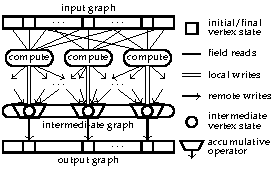
\includegraphics[width=0.9\textwidth]{figures/model.pdf}
 \vspace{-2ex}
 \caption{In an algorithmic superstep, every vertex performs local computation (including field reads and local writes) and remote updating in order.}
 \label{fig:algostep}
\end{figure}

More precisely, an algorithmic superstep is divided into two phases:
\begin{itemize}
 \item a \emph{local computation} (LC) phase, in which a copy of the input graph is created as the intermediate graph, and then each vertex can read the state of any vertex in the input graph, perform local computation, and modify its own state in the intermediate graph, and
 \item a \emph{remote updating} (RU) phase, in which each vertex can modify the states of any vertices in the intermediate graph by sending remote writes.
After all remote writes are processed, the intermediate graph is returned as the output graph.
\end{itemize}
Among these two phases, the RU phase is optional, in which case the intermediate graph produced by the LC phase is used directly as the final result.

\begin{comment}
Second, it clearly splits a piece of computation into three phases where local and remote writes are executed separately, avoiding synchronization issues.
It also gives programmers a standard template to describe vertex-centric computation. \todo{why is this good?}
Third, the high-level semantics makes it easier to transform algorithmic supersteps into efficient Pregel code. \todo{combine with the first point?}
Second, an algorithmic superstep contains both remote reads or writes,
First, it allows a vertex to update other vertices at the end of a superstep, which is also a common and necessary pattern of communication in graph algorithms. \todo{also looks like a motivation. integrate this with the paragraph above?}
\end{comment}

%On top of algorithmic supersteps, we further define two operations called \textit{sequence} and \textit{iteration}.
%Thus, algorithmic supersteps can be composed, or iteratively executed until certain condition is satisfied.

\subsection{An overview of Palgol}
\label{sec:palgol-syntax}

Next we present Palgol, whose design follows the high-level model we introduced above.
Figure~\ref{fig:syntax-simplified} shows the essential part of Palgol's syntax.
%(A few more constructs will be introduced in Section~\ref{sec:advanced}.)
As described by the syntactic category \textit{step}, an algorithmic superstep in Palgol is a code block
enclosed by ``\textbf{for} \textit{var} \textbf{in} \textbf{V}'' and ``\textbf{end}'', where \textit{var} is a variable name that can be used in the code block for referring to the current vertex (and \textbf{V} stands for the set of vertices of the input graph).
Such steps can then be composed (by sequencing) or iterated until a termination condition is met (by enclosing them in ``\textbf{do}'' and ``\textbf{until} \ldots'').
Palgol supports several kinds of termination condition, but in this thesis we focus on only one kind of termination condition called \textit{fixed point}, since it is extensively used in many algorithms.
The semantics of fixed-point iteration is iteratively running the program enclosed by \textbf{do} and \textbf{until}, until the specified fields stabilize.
%\todo{perhaps mention there are others}

\begin{figure}[t]
\normalsize
\[
\begin{array}{lclr}
%\mathit{int} & = & \hbox{integer} \\
%\mathit{float} & = & \hbox{floating-point number} \\
%\mathit{var} & = & \hbox{identifier starting with lowercase letter} \\
%\mathit{field} & = & \hbox{identifier starting with capital letter} \\
%\\
\mathit{prog}  & \Coloneqq & \mathit{step}~|~\mathit{prog_1}\ldots\mathit{prog_n}~|~\mathit{iter} \\
\mathit{iter} & \Coloneqq & \mathbf{do}~\langle~\mathit{prog}~\rangle~\mathbf{until}~\mathbf{fix}~[~\mathit{field_1},\ldots,\mathit{field_n}~] \\
\mathit{step}& \Coloneqq & \mathbf{for}~\mathit{var}~\mathbf{in}~\mathbf{V}~\langle~\mathit{block}~\rangle~\mathbf{end} \\
\mathit{block} & \Coloneqq & \mathit{stmt_1} \ldots \mathit{stmt_n} \\
\mathit{stmt}  & \Coloneqq & \mathbf{if}~\mathit{exp}~\langle~\mathit{block}~\rangle~|~\mathbf{if}~\mathit{exp}~\langle~\mathit{block}~\rangle~\mathbf{else}~\langle~\mathit{block}~\rangle \\
 & | & \mathbf{for}~(\mathit{var}\leftarrow\mathit{exp})~\langle~\mathit{block}~\rangle \\
 & | & \mathbf{let}~\mathit{var}=\mathit{exp} \\
 & | & \mathbf{local}\mathit{_{opt}}~\mathit{field}~[~\mathit{var}~]~\mathit{op_{local}}~\mathit{exp} & \hsp{-- local write} \\
 & | & \mathbf{remote}~\mathit{field}~[~\mathit{exp}~]~\mathit{op_{remote}}~\mathit{exp} & \hsp{-- remote write} \\
\mathit{exp}   & \Coloneqq & \mathit{int}~|~\mathit{float}~|~\mathit{var}~|~\mathbf{true}~|~\mathbf{false}~|~\mathbf{inf} \\
 & | & \mathbf{fst}~\mathit{exp}~|~\mathbf{snd}~\mathit{exp}~|~(\mathit{exp},\mathit{exp}) \\
 & | & \mathit{exp}.\mathbf{ref}~|~\mathit{exp}.\mathbf{val}~|~\{\mathit{exp},\mathit{exp}\}~|~\{\mathit{exp}\} & \hsp{-- specialized pair} \\
 & | & \mathit{exp}~?~\mathit{exp}:\mathit{exp}~|~(~\mathit{exp}~)~|~\mathit{exp}~\mathit{op_{b}}~\mathit{exp}~|~\mathit{op_{u}}~\mathit{exp} \\
 & | & \mathit{field}~[~\mathit{exp}~] & \hsp{-- global field access} \\
 & | & \mathit{func_{opt}}~[~\mathit{exp}~|~\mathit{var}\leftarrow\mathit{exp},\mathit{exp_1},\ldots,\mathit{exp_n}~] \\
\mathit{func}  & \Coloneqq & \mathbf{maximum}~|~\mathbf{minimum}~|~\mathbf{sum}~|~\ldots \\
 \end{array}
\]
\vspace{-2ex}
\caption{Essential part of Palgol's syntax. Palgol is indentation-based, and two special tokens `$\langle$' and `$\rangle$' are introduced to delimit indented blocks.}
\label{fig:syntax-simplified}
\end{figure}

%As mentioned before, an algorithmic superstep has two phases, local computation (LC) and remote updating (RU).
Corresponding to an algorithmic superstep's remote access capabilities, in Palgol we can read a field of an arbitrary vertex using a global field access expression of the form $\mathit{field}~[\,\mathit{exp}\,]$, 
where $\mathit{field}$ is a user-specified field name and $\mathit{exp}$ should evaluate to a vertex id.
Such expression can be updated by local or remote assignments, where an assignment to a remote vertex should always be accumulative and prefixed with the keyword $\mathbf{remote}$.
%and use accumulative assignment operation only.
One more thing about remote assignments is that they take effect only in the RU phase (after the LC phase), regardless of where they occur in the program.
%Such syntax looks similar to an array access, and indeed, one can regard a field as a global array, so that when a vertex id is given, the value of the field on that vertex is returned.
%In Palgol, we can also update a remote field using an accumulative assignment statement prefixed with the keyword $\mathbf{remote}$.
%Remote updating statements take effect only in the RU phase (after the LC phase), regardless of where they occur in the program, and the assignment operation can only be accumulative.
%To better distinguish the two kinds of updating statements, local updating statements are prefixed with the \textbf{local} keyword.
%\end{itemize}

There are some predefined fields that have special meaning in our language.
%$\mathbf{Nbr}$, $\mathbf{In}$, $\mathbf{Out}$ are by default the edge lists, where 
$\mathbf{Nbr}$ is the edge list in undirected graphs, and $\mathbf{In}$ and $\mathbf{Out}$ respectively store incoming and outgoing edges for directed graphs.
Essentially, these are normal fields of a predefined type for representing edges, and most importantly, the compiler assumes a form of symmetry on these fields (namely that every edge is stored consistently on both of its end vertices), and uses the symmetry to produce more efficient code.
%Then, $\mathbf{Id}$ is an immutable field that stores the vertex identifier for each vertex (required by the Pregel framework), whose type is user-specified but currently we can simply treat it as an integer.

The rest of the syntax for Palgol steps is similar to an ordinary programming language.
Particularly, we introduce a specialized pair type (expressions in the form of $\{\mathit{exp},\mathit{exp}\}$) for representing a reference with its corresponding value (e.g., an edge in a graph), and use $.\mathbf{ref}$ and $.\mathbf{val}$ respectively to access the reference and the value respectively, to make the code easy to read.
Some functional programming constructs are also used here, like let-binding and list comprehension.
There is also a foreign function interface that allows programmers to invoke functions written in a general-purpose language, but we omit the detail from the paper.

\subsection{Case studies}

Next, we use two examples to show how to use Palgol to implement graph algorithms.

\subsubsection{The Shiloach-Vishkin Connected Component Algorithm}
\label{sec:sv-algorithm}

Here is our first representative Palgol example: the \emph{Shiloach-Vishkin (SV) connected component algorithm}~\cite{yan2015effective}, which can be expressed as the Palgol program in \autoref{fig:svppa-code}.
%to show how to describe vertex-centric algorithms in Palgol.
%This algorithm uses many interesting features in Palgol.
A traditional HashMin connected component algorithm~\cite{yan2015effective} based on neighborhood communication takes time proportional to the input graph's diameter, which can be large in real-world graphs.
In contrast, the SV algorithm can calculate the connected components of an undirected graph in a logarithmic number of supersteps; to achieve this fast convergence, the capability of accessing data on non-neighboring vertices is essential.

In the SV algorithm, the connectivity information is maintained using the classic disjoint set data structure~\cite{disjointset}.
Specifically, the data structure is a forest, and vertices in the same tree are regarded as belonging to the same connected component.
Each vertex maintains a parent pointer that either points to some other vertex in the same connected component, or points to itself, in which case the vertex is the root of a tree.
We henceforth use $D[u]$ to represent this pointer for each vertex $u$.
The SV algorithm is an iterative algorithm that begins with a forest of $n$ root nodes, and in each step it tries to discover edges connecting different trees and merge the trees together.
In a vertex-centric way, every vertex~$u$ performs one of the following operations depending on whether its parent $D[u]$ is a root vertex:
\begin{itemize}
 \item \textbf{tree merging:}
  if $D[u]$ is a root vertex, then $u$ chooses one of its neighbors' current parent (to which we give a name $t$), and makes $D[u]$ point to $t$ if $t<D[u]$ (to guarantee the correctness of the algorithm).
  When having multiple choices in choosing the neighbors' parent $p$, or when different vertices try to modify the same parent vertex's pointer, the algorithm always uses the ``minimum'' as the tiebreaker for fast convergence.
 \item \textbf{pointer jumping:}
  if $D[u]$ is not a root vertex, then $u$ modifies its own pointer to its current ``grandfather'' ($D[u]$'s current pointer).
  This operation reduces $u$'s distance to the root vertex, and will eventually make~$u$ a direct child of the root vertex so that it can perform the above tree merging operation.
\end{itemize}
The algorithm terminates when all vertices' pointers do not change after an iteration, in which case all vertices point to some root vertex and no more tree merging can be performed.
Readers interested in the correctness of this algorithm are referred to the original paper~\cite{yan2015effective} for more details.

\begin{comment}
 \KwInput{an undirected graph}
 \KwOutput{connected components represented as the root id of each disjoint sets}
 \BlankLine
 \emph{every vertex initializes a pointer pointing to itself}\;
 \Repeat{the disjoint-set structure does not change}{
  \For{each vertex $u$}{
   \eIf {$u$'s parent is a root node}{
    \emph{choose a neighbor~$v$ whose parent's id is smaller than $u$'s parent's id}\;
    \emph{if $v$ exists, make $u$'s parent point to $v$'s parent}\;
   }{
    \emph{make $u$ point to its grandparent}\;
   }
  }
 }
 \BlankLine
 \caption{The SV algorithm description}
 \label{fig:svppa-desc}
\end{comment}

The implementation of this algorithm is complicated, which contains roughly 120 lines of code\footnote{\url{http://www.cse.cuhk.edu.hk/pregelplus/code/apps/basic/svplus.zip}} for the $\textit{compute()}$ function alone.
Even for detecting whether the parent vertex $D[u]$ is a root vertex for each vertex $u$, it has to be translated into three supersteps containing a query-reply conversation between each vertex and its parent.
%Here we just explain the message-passing-based Pregel implementation of a small part of the algorithm, to give a sense of its complexity.
%For example, $u$~needs to know whether its parent~$p$ is a root node or not, i.e., whether $p$'s pointer points to $p$~itself.
%The implementation achieves this by making~$p$ send its pointer to~$u$ in a previous superstep, so that $u$~can check whether $p$'s pointer points to~$p$.
%Moreover, since $p$~does not maintain a list of its children, $u$~must send its own id to~$p$ in an additional superstep before $p$~sends its pointer.
%In the next superstep, when $p$~receives all the ids of its children, it will reply its pointer to them, and in the third superstep, $u$~will finally obtain the information it needs and decide which branch to go.
%We can see that, despite the simplicity of the description at algorithm level, it has to be translated into three supersteps containing a query-reply conversation between each vertex and its parent.
In contrast, the Palgol program in Figure \ref{fig:svppa-code} can describe this algorithm concisely in 13 lines, due to the declarative remote access syntax.
This piece of code contains two steps, where the first one (lines 1--3) performs simple initialization, and the other (lines 5--12) is inside an iteration as the main computation.
We also use the field~$D$ to store the pointer to the parent vertex.
%\footnote{In Palgol, vertices' fields are represented by identifiers starting with a capital letter.}.
Let us focus on line~6, which checks whether $u$'s parent is a root.
Here we simply check $D[D[u]] \shorteqq D[u]$, i.e., whether the pointer of the parent vertex $D[D[u]]$ is equal to the parent's id $D[u]$.
This expression is completely declarative, in the sense that we only specify what data is needed and what computation we want to perform, instead of explicitly implementing the message passing scheme.
%All the magic happens in our compilation algorithm, which analyzes the expression and generates the message passing code.
%The first algorithmic superstep is actually very simple, which set each vertex's $D$ field to the vertex's own id.
%In our type system, $u$ and $D$ field have a special type called \textit{vertex id} or \textbf{vid} for short, and this type is mainly used in the statements or expressions involving data communication.

\begin{figure}[t]
\begin{lstlisting}[basicstyle=\small\ttfamily]
for u in V
  D[u] := u
end
do
  for u in V
    if (D[D[u]] == D[u])
      let t = minimum [ D[e.ref] | e <- Nbr[u] ]
      if (t < D[u])
        remote D[D[u]] <?= t
    else
      D[u] := D[D[u]]
  end
until fix[D]
\end{lstlisting}
\vspace{-2ex}
\caption{The SV algorithm in Palgol}
\label{fig:svppa-code}
\end{figure}

The rest of the algorithm can be straightforwardly associated with the Palgol program.
If $u$'s parent is a root, we generate a list containing all neighboring vertices' parent id ($D[e.\mathbf{ref}]$), and then bind the minimum one to the variable~$t$ (line~7).
Now $t$~is either \textbf{inf} if the neighbor list is empty or a vertex id; in both cases we can use it to update the parent's pointer (lines 8--9) via a remote assignment.
One important thing is that the parent vertex ($D[u]$) may receive many remote writes from its children, where only one of the children providing the minimum $t$ can successfully perform the updating.
Here, the statement \texttt{a <?= b} is an accumulative assignment, whose meaning is the same as \texttt{a := min(a, b)}.
%\todo{typeset the operators}
Finally, for the $\mathbf{else}$ branch, we (locally) assign $u$'s grandparent's id to $u$'s $D$ field.

%The SV program demonstrates how programmers can naturally describe a complex Pregel algorithm in Palgol, in particular using the field access syntax and the remote updating syntax.
%Later we will see how such a Palgol program can be efficiently compiled into an efficient Pregel program.

\subsubsection{The List Ranking Algorithm}
\label{sec:list-ranking}

Another example is the \emph{list ranking} algorithm, which also needs communication over a dynamic structure during computation.
Consider a linked list~$L$ with $n$~elements, where each element $u$ stores a value $\mathit{val}(u)$ and a link to its predecessor $\mathit{pred}(u)$.
At the head of $L$ is a virtual element~$v$ such that $\mathit{pred}(v)=v$ and $\mathit{val}(v)=0$.
For each element~$u$ in~$L$, define $\mathit{sum}(u)$ to be the sum of the values of all the elements from~$u$ to the head (following the predecessor links).
The list ranking problem is to compute $\mathit{sum}(u)$ for each element $u$.
If $\mathit{val}(u)=1$ for every vertex~$u$ in~$L$, then $\mathit{sum}(u)$ is simply the rank of~$u$ in the list.
List ranking can be solved using a typical pointer-jumping algorithm in parallel computing with a strong performance guarantee.
Yan~et~al.~\cite{yan2015effective} demonstrated how to compute the pre-ordering numbers for all vertices in a tree in $O(\log n)$ supersteps using this algorithm, as an internal step to compute bi-connected components (BCC).%
\footnote{BCC is a complicated algorithm, whose efficient implementation requires constructing an intermediate graph, which is currently beyond Palgol's capabilities. Palgol is powerful enough to express the rest of the algorithm, however.}

\begin{figure}[t]
\begin{lstlisting}[basicstyle=\small\ttfamily]
for u in V
  Sum[u] := Val[u]
end
do
  for u in V
    if (Pred[Pred[u]] != Pred[u])
      Sum[u] += Sum[Pred[u]]
      Pred[u] := Pred[Pred[u]]
  end 
until fix[Pred]
\end{lstlisting}
\vspace{-2ex}
\caption{The list ranking program}
\label{fig:ranking-code}
\end{figure}

We give the Palgol implementation of list ranking in~\autoref{fig:ranking-code} (which is a 10-line program, whereas the Pregel implementation\footnote{\url{http://www.cse.cuhk.edu.hk/pregelplus/code/apps/basic/bcc.zip}} contains around 60~lines of code).
$\mathit{Sum}[u]$ is initially set to\,$\mathit{Val}[u]$ for every~$u$ at line~2; inside the fixed-point iteration (lines 5--9), every~$u$ moves $\mathit{Pred}[u]$ toward the head of the list and updates $\mathit{Sum}[u]$ to maintain the invariant that $\mathit{Sum}[u]$ stores the sum of a sublist from itself to the successor of $\mathit{Pred}[u]$.
Line~6 checks whether $u$~points to the virtual head of the list, which is achieved by checking $\mathit{Pred}[\mathit{Pred}[u]] \shorteqq \mathit{Pred}[u]$, i.e., whether the current predecessor $\mathit{Pred}[u]$ points to itself.
If the current predecessor is not the head, we add the sum of the sublist maintained in $\mathit{Pred}[u]$ to the current vertex~$u$, by reading $\mathit{Pred}[u]$'s $\mathit{Sum}$ and $\mathit{Pred}$ fields and modifying $u$'s own fields accordingly.
Note that since all the reads are performed on a snapshot of the input graph and the assignments are performed on an intermediate graph, there is no need to worry about data dependencies.

\section{Compiling Palgol to Pregel}
\label{sec:compilation}

In this section, we present the compiling algorithm to transform Palgol to Pregel.
The task overall is complicated and highly technical, but the most challenging problem is how to translate chain access (like $D[D[u]]$) into Pregel's message passing model.
%and how to implement sequence and iteration, which will be presented in \autoref{sec:trans-step} and \autoref{sec:trans-iter} respectively.
%When compiling a single Palgol step, the most challenging part is the remote reads, for which we first give a detailed explanation in \autoref{sec:trans-chain}.
We describe the compilation of chain access in \autoref{sec:trans-chain}, and then the compilation of a Palgol step in \autoref{sec:trans-step}, and finally how to combine Palgol steps using sequence and iteration in \autoref{sec:trans-iter}.

\subsection{Compiling remote reads}
\label{sec:trans-chain}

Our compiler currently recognizes two forms of remote reads.
The first form is \emph{chain access} expressions like $D[D[u]]$.
The second form is \emph{neighborhood access} where a vertex may use chain access to acquire data from \emph{all} its neighbors, and this can be described using the list comprehension (e.g., line~7 in \autoref{fig:svppa-code}) or for-loop syntax in Palgol.
The combination of these two remote read patterns is already sufficient to express quite a wide range of practical Pregel algorithms.
%according to our experience. %(see the discussion in \autoref{sec:related}).
Here we only present the compilation of chain access, which is novel, while the compilation of neighborhood access is similar to what has been done in Fregel.

\subsubsection{Definition and challenge of compiling:}
A chain access is a consecutive field access expression starting from the current vertex.
As an example, supposing that the current vertex is~$u$, and $D$~is a field for storing a vertex id, then $D[D[u]]$ is a chain access expression, and so is $D[D[D[D[u]]]]$ (which we abbreviate to $D^4[u]$ in the rest of this section).
Generally speaking, there is no limitation on the depth of a chain access or the number of fields involved in the chain access.

As a simple example of the compilation, to evaluate $D[D[u]]$ on every vertex~$u$, a straightforward scheme is a request-reply conversation which takes two rounds of communication:
in the first superstep, every vertex~$u$ sends a request to (the vertex whose id is) $D[u]$ and the request message should contain $u$'s own id;
then in the second superstep, those vertices receiving the requests should extract the sender's ids from the messages, and reply its $D$ field to them.

When the depth of such chain access increases, it is no longer trivial to find an efficient scheme, where efficiency is measured in terms of the number of supersteps taken.
For example, to evaluate $D^4[u]$ on every vertex $u$, a simple query-reply method takes six rounds of communication by evaluating $D^2[u]$, $D^3[u]$ and $D^4[u]$ in turn, each taking two rounds, but the evaluation can actually be done in only three rounds with our compilation algorithm, which is not based on request-reply conversations.
%To this problem, we build a novel transformation algorithm, in which such scheme is easy to obtain.

\subsubsection{Logic system for compiling chain access:}
The key insight leading to our compilation algorithm is that we should consider not only the expression to evaluate but also the vertex on which the expression is evaluated.
To use a slightly more formal notation (inspired by Halpern and Moses~\cite{Halpern-common-knowledge}), we write $\forall u.\,\knows{v(u)}{e(u)}$, where $v(u)$~and~$e(u)$ are chain access expressions starting from~$u$, to describe the state where every vertex $v(u)$ ``knows'' the value of the expression $e(u)$; then the goal of the evaluation of $D^4[u]$ can be described as $\forall u.\,\knows{u}{D^4[u]}$.
%which means that we want to finally achieve the state that every vertex $u$ knows the result of $D^4[u]$.
Having introduced the notation, the problem can now be treated from a logical perspective, where we aim to search for a derivation of a target proposition from a few axioms.

There are three axioms in our logic system:
\begin{enumerate}
\item $\forall u.\,\knows{u}{u}$
\item $\forall u.\,\knows{u}{\mathit{D}[u]}$
\item $(\forall u.\,\knows{w(u)}{e(u)}) \wedge (\forall u.\,\knows{w(u)}{v(u)}) \implies \forall u.\,\knows{v(u)}{e(u)}$
\end{enumerate}
The first axiom says that every vertex knows its own id, and the second axiom says every vertex can directly access its local field $D$.
The third axiom encodes message passing: if we want every vertex $v(u)$ to know the value of the expression $e(u)$, then it suffices to find an intermediate vertex $w(u)$ which knows both the value of $e(u)$ and the id of $v(u)$, and thus can send the value to $v(u)$.
% suppose that every vertex~$x$ knows some value~$a$, and it also knows the vertex $b$, then if all $x$ sends the value $a$ to vertex $b$, then all vertex $b$ will holds the value $a$.
As an example, Figure~\ref{fig:d4u-rules} shows the solution generated by our algorithm to solve $\forall u.\,\knows{u}{D^4[u]}$, where each line is an instance of the message passing axiom.

\begin{figure}[t]
\normalsize
\begin{align*}
(\forall u.\,\knows{\mathrlap{u}\phantom{D^2[u]}}{\mathrlap{u}\phantom{D^2[u]}}) \mathrel\wedge (\forall u.\,\knows{\mathrlap{u}\phantom{D^2[u]}}{\mathrlap{D[u]}\phantom{D^2[u]}}) &\implies \forall u.\,\knows{\mathrlap{D[u]}\phantom{D^2[u]}}{u} \\
(\forall u.\,\knows{\mathrlap{D[u]}\phantom{D^2[u]}}{\mathrlap{u}\phantom{D^2[u]}}) \mathrel\wedge (\forall u.\,\knows{\mathrlap{D[u]}\phantom{D^2[u]}}{D^2[u]}) &\implies \forall u.\,\knows{\mathrlap{D^2[u]}\phantom{D^2[u]}}{u} \\
(\forall u.\,\knows{\mathrlap{D[u]}\phantom{D^2[u]}}{D^2[u]}) \mathrel\wedge (\forall u.\,\knows{\mathrlap{D[u]}\phantom{D^2[u]}}{\mathrlap{u}\phantom{D^2[u]}}) &\implies \forall u.\,\knows{\mathrlap{u}\phantom{D^2[u]}}{D^2[u]} \\
%[D(D(u))]_u & & & \implies & [D(D(D(D(u))))]_{D(D(u))} \\
(\forall u.\,\knows{\mathrlap{D^2[u]}\phantom{D^2[u]}}{D^4[u]}) \mathrel\wedge (\forall u.\,\knows{\mathrlap{D^2[u]}\phantom{D^2[u]}}{\mathrlap{u}\phantom{D^2[u]}}) &\implies \forall u.\,\knows{\mathrlap{u}\phantom{D^2[u]}}{D^4[u]}
\end{align*}
\vspace{-4ex}
\caption{A derivation of $\forall u.\,\knows{u}{D^4[u]}$}
\label{fig:d4u-rules}
\end{figure}

\autoref{fig:d4u-msg} is a direct interpretation of the implications in \autoref{fig:d4u-rules}.
To reach $\forall u.\,\knows{u}{D^4[u]}$, only three rounds of communication are needed.
Each solid arrow represents an invocation of the message passing axiom in Figure~\ref{fig:d4u-rules}, and the dashed arrows represent two logical inferences, one from $\forall u.\,\knows{u}{D[u]}$ to $\forall u.\,\knows{D[u]}{D^2[u]}$ and the other from $\forall u.\,\knows{u}{D^2[u]}$ to $\forall u.\,\knows{D^2[u]}{D^4[u]}$.
%Note that the number of rounds is reduced to three since we can derive both $\forall u.\,\knows{u}{D^2[u]}$ and $\forall u.\,\knows{D^2[u]}{u}$ in $S3$.
%we finally get the $\forall u.\,\knows{u}{D^4[u]}$.

\begin{figure}[t]
 \centering
 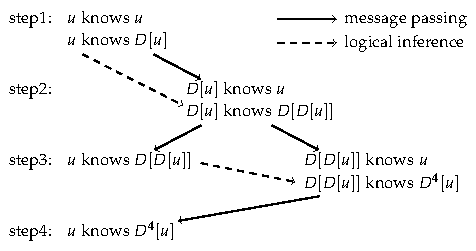
\includegraphics[width=0.75\textwidth]{figures/d4u.pdf}
 \vspace{-2ex}
 \caption{Interpretation of the derivation of $\forall u.\,\knows{u}{D^4[u]}$}
 \label{fig:d4u-msg}
\end{figure}

The derivation of $\forall u.\,\knows{u}{D^4[u]}$ is not unique, and there are derivations that correspond to inefficient solutions --- for example, there is also a derivation for the six-round solution based on request-reply conversations.
However, when searching for derivations, our algorithm will minimize the number of rounds of communication, as explained below.

\subsubsection{The compiling algorithm:}
Initially, the algorithm sets as its target a proposition $\forall u.\,\knows{v(u)}{e(u)}$, for which a derivation is to be found.
%Later we will show that only considering these two patterns is enough.
The key problem here is to choose a proper $w(u)$ so that, by applying the message passing axiom backwards, we can get two potentially simpler new target propositions $\forall u.\,\knows{w(u)}{e(u)}$ and $\forall u.\,\knows{w(u)}{v(u)}$ and solve them respectively.
The range of such choices is in general unbounded, but our algorithm considers only those simpler than $v(u)$ or $e(u)$.
More formally, we say that $a$~is a \emph{subpattern} of~$b$, written $a \preceq b$, exactly when $b$~is a chain access starting from~$a$.
%i.e., $b = \vec C[a]$ for a (possibly empty) chain $\vec C$ of fields.
For example, $u$~and $D[u]$ are subpatterns of $D[D[u]]$, while they are all subpatterns of $D^3[u]$.
The range of intermediate vertices we consider is then $\mathrm{Sub}(e(u), v(u))$, where $\mathrm{Sub}$ is defined by
\[ \mathrm{Sub}(a, b) = \{\,c \mid c \preceq a \mathrel\text{or} c \prec b \,\} \]
We can further simplify the new target propositions with the following function before solving them:
\[
\mathit{generalize}(\forall u.\,\knows{a(u)}{b(u)}) =
\begin{cases}
\forall u.\,\knows{u}{(b(u)/a(u))} & \text{if~} a(u) \preceq b(u) \\
\forall u.\,\knows{a(u)}{b(u)} & \text{otherwise}
\end{cases}
\]
where $b(u)/a(u)$ denotes the result of replacing the innermost $a(u)$ in $b(u)$ with~$u$.
(For example, $A[B[C[u]]]/C[u] = A[B[u]]$.)
This is justified because the original proposition can be instantiated from the new proposition.
(For example, $\forall u.\,\knows{C[u]}{A[B[C[u]]]}$ can be instantiated from $\forall u.\,\knows{u}{A[B[u]]}$.)

It is now possible to find an optimal solution with respect to the following inductively defined function $\mathit{step}$, which calculates the number of rounds of communication for a proposition:
\[ \setlength{\arraycolsep}{.2em}\begin{array}{lcl}
\mathit{step}(\forall u.\,\knows{u}{u}) &=& 0 \\
\mathit{step}(\forall u.\,\knows{u}{\mathit{D}[u]}) &=& 0 \\
\mathit{step}(\forall u.\,\knows{v(u)}{e(u)}) &=& \displaystyle 1+ \min_{w(u)\in \mathrm{Sub}(e(u),v(u))}~\max(x, y) \\
\multicolumn{3}{l}{\quad\text{where}~x = \mathit{step}(\mathit{generalize}(\forall u.\,\knows{w(u)}{e(u)}))} \\
\multicolumn{3}{l}{\quad\phantom{\text{where}}~y = \mathit{step}(\mathit{generalize}(\forall u.\,\knows{w(u)}{v(u)}))}
\end{array} \]
It is straightforward to see that this is an optimization problem with optimal and overlapping substructure, which we can solve efficiently with memoization techniques.

With this compiling algorithm, we are now able to handle any chain access expressions.
Furthermore, this algorithm optimizes the generated Pregel program in two aspects.
First, this algorithm derives a message passing scheme with a minimum number of supersteps, thus reduces unnecessary cost for launching Pregel supersteps during execution.
Second, by extending the memoization technique, we can ensure that a chain access expression will be evaluated exactly once even if it appears multiple times in a Palgol step, avoiding redundant message passing for the same value.

\begin{comment}
\subsubsection{neighborhood access}
\label{sec:neighboring-access}

%In the previous subsection, we have shown that a particular form of remote access, i.e., consecutive field access expressions starting from the current vertex, can be efficiently compiled to message passing by using our inference system and the searching algorithm.
neighborhood access is another important communication pattern widely used in Pregel algorithms.
Precisely speaking, neighborhood access refers to those chain access expressions inside a non-nested loop traversing an edge list (\textbf{Nbr}, \textbf{In} or \textbf{Out}), where the chain access expressions start from the neighboring vertex.
The following code is a typical example of neighborhood access, which is a list comprehension used in the SV algorithm program (Figure~\ref{fig:svppa-code}):
\begin{lstlisting}[basicstyle=\footnotesize,firstnumber=7]
    let t = minimum [ D[e.id] | e <- Nbr[v] ]
\end{lstlisting}
Syntactically, a field access expression $D[e.\mathbf{ref}]$ can be easily identified as a neighborhood access.

The compilation of such data access pattern is based on the symmetry that if \emph{all} vertices need to fetch the same field of their neighbors, that will be equivalent to making all vertices send the field to all their neighbors.
This is a well-known technique that is also adopted by Green-Marl and Fregel, so we do not go into the details and simply summarize the compilation procedure as follows:
\begin{enumerate}
 \item In the first superstep, we prepare the data from neighbors' perspective.
  Field access expressions like $D[e.\mathbf{ref}]$ now become neighboring vertices' local fields $D[u]$.
  %In general, chain access like $D[D[e.\mathbf{ref}]]$ can be transformed to $D[D[u]]$, which is then evaluated by using the algorithm shown in \autoref{sec:trans-chain}.
 Every vertex then sends messages containing those values to all its neighboring vertices.
 \item In the next step, every vertex scans the message list to obtain all the values of neighborhood access, and then executes the loop according to the Palgol program.
\end{enumerate}

% resulting in a sending superstep and a receiving superstep, taking only a single round of communication.
%Essentially, what it achieves is to translate (starting from $e.\mathbf{ref}$) from the current vertex $v$'s perspective to \emph{local} field access expressions (starting from the current vertex) from neighbors' perspective, so that they can be easily translated to message passing by the algorithm in Section~\ref{sec:trans-chain}.
\end{comment}

\subsection{Compiling Palgol steps}
\label{sec:trans-step}

Having introduced the compiling algorithm for remote data reads in Palgol, here we give a general picture of the compilation for a single Palgol step, as shown in \autoref{fig:compiling-Palgol-step}.
The computational content of every Palgol step is compiled into a \emph{main superstep}.
Depending on whether there are remote reads and writes, there may be a number of \emph{remote reading supersteps} before the main superstep, and a \emph{remote updating superstep} after the main superstep.

\begin{figure}[t]
 \centering
 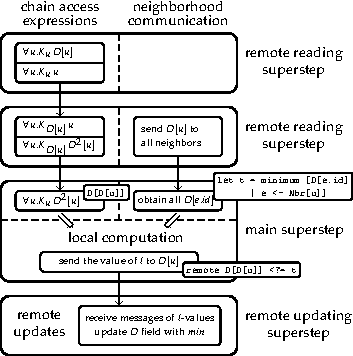
\includegraphics[width=0.75\textwidth]{figures/compile.pdf}
 \vspace{-2ex}
 \caption{Compiling a Palgol step to Pregel supersteps.}
 \label{fig:compiling-Palgol-step}
\end{figure}

We will use the main computation step of the SV program (lines 5--12 in \autoref{fig:svppa-code}) as an illustrative example for explaining the compilation algorithm, which consists of the following four steps:
% \todo{emphasize the order?}
\begin{enumerate}

\item We first handle neighborhood access, which requires a sending superstep that provides all the remote data for the loops from the neighbors' perspective. % (for SV algorithm, sending their $D$~field to all their neighbors).
This sending superstep is inserted as a remote reading superstep immediately before the main superstep.

\item We analyze the chain access expressions appearing in the Palgol step with the algorithm in \autoref{sec:trans-chain}, and corresponding remote reading supersteps are inserted in the front.
(For the SV algorithm, the only interesting chain access expression is $D[D[u]]$, which induces two remote reading supersteps realizing a request-reply conversation.)
%In addition, our handling of neighborhood access may introduce more chain accesses in the sending superstep, and message passing schemes should also be generated for those accesses.
%(For SV algorithm, the chain access introduced by neighborhood access is $D[u]$, which happens to be trivial.)

%Messages for different loops are attached with different tags, so in the computation step, we can easily distinguish the messages.
%After that, the program will contains only the (consecutive) field access expressions starting from the current vertex, so the transformation system introduced in Section~\ref{sec:trans-chain} is used to further translate them to message passing.
%A simple optimization is that, the same chain access expression in an algorithmic superstep should only be evaluated once, then all occurence of the expression can refer to the same value.
%During the translation of chain access expressions, some more supersteps may be inserted to the program to propagate information between vertices, and a simple dependency analysis is used to minimize the total number of supersteps.

\item Having handled all remote reads, the main superstep receives all the values needed and proceeds with the local computation.
Since the local computational content of a Palgol step is similar to an ordinary programming language, the transformation is straightforward.
%According to the semantics described in \autoref{sec:syntax}, a local updating statement is actually a deferred assignment, which always takes place when all local computation is done.
%In general, we need to create a separate copy of all the involved fields at the beginning of the superstep.
%Then, during the superstep, all field reads are performed on the original fields, and all updates are on the copies.
%Finally, we use the (possibly updated) values of the copies to update the original fields at the end of the superstep.
%A simple optimization is to check whether in an algorithmic a field has data access after updates, so that some duplication can be avoided.

\item What remain to be handled are the remote assignments, which require sending the updating values as messages to the target vertices in the main superstep.
%(For SV algorithm, there is one remote updating statement at line 10, requiring that the value of~$t$ be sent to $D[u]$.)
Then an additional remote updating superstep is added after the main superstep; this additional superstep reads these messages and updates each field using the corresponding remote updating operator.
%(For SV algorithm, the minimum of all the $t$-values received is assigned to field~$D$.)
\end{enumerate}

\subsection{Compiling sequences and iterations}
\label{sec:trans-iter}

Finally, we look at the compilation of sequence and iteration, which assemble Palgol steps into larger programs.
A Pregel program generated from Palgol code is essentially a \emph{state transition machine} (STM) combined with computation code for each state.
Every Palgol step is translated into a ``linear'' STM consisting of a chain of states corresponding to the supersteps like those shown in \autoref{fig:compiling-Palgol-step},
%but in general, a generated STM can have more complicated structures between its start state and end state, due to the iteration constructs in Palgol.
and the compilation of a Palgol program starts from turning the atomic Palgol steps into linear STMs, and implements the sequence and iteration semantics to construct more complex STMs.

\textbf{Compilation of sequence}:
%A sequence of two Palgol programs uses the first program to transform an initial graph to an intermediate one, which is then transformed to a final graph using the second program.
To compile the sequence, we first compile the two component programs into STMs, then a composite STM is constructed by simply adding a state transition from the end state of the first STM to the start state of the second STM.

\textbf{Compilation of iteration}:
%A fixed-point iteration repeatedly runs a program enclosed by `\textbf{do}' and `\textbf{until} \ldots' until the specified fields stabilize.
We first compile the loop body into an STM, which starts from some state $S_\mathit{start}$ and ends in a state $S_\mathit{end}$, then we extend this STM to implement the fixed-point semantics.
Here we describe a generalized approach which generates a new STM starting from state $S_\mathit{start'}$ and ending in state $S_\mathit{end'}$:

\begin{enumerate}
 \item 
  First, a check of the termination condition takes place right before the state $S_\mathit{start}$: if it holds, we immediately enters a new exit state $S_\mathit{exit'}$; otherwise we execute the body, after which we go back to the check by adding a state transition from $S_\mathit{end}$ to $S_\mathit{start}$.
  This step actually implements a while loop.
 \item
  The termination check is implemented by an OR aggregator to make sure that every vertex makes the same decision:
  basically, all vertices determine whether their local fields stabilize during a single iteration by storing the original values beforehand, and the aggregator combines the results and makes it available to all vertices.
 \item
  We add a new start state $S_\mathit{start'}$ and make it directly transit to $S_\mathit{start}$.
  This state is for storing the original values of the fields, and also to make the termination check succeed in the first run, turning the while loop into a do-until loop.
\end{enumerate}

\textbf{Optimizations}:
In the compilation of sequence and iteration, two optimization techniques are used to reduce the number of states in the generated STMs and can remove unnecessary synchronizations.
Due to space restrictions, we will not present all the details here, but these techniques share similar ideas with Green-Marl's ``state merging'' and ``intra-loop state merging'' optimizations~\cite{green14}:
\begin{itemize}
 \item \emph{state merging}:
  whenever it is safe to do so, the Green-Marl compiler merges two consecutive states of vertex computation into one.
  In the compilation of sequence in Palgol, we can always safely merge the end state of the first STM and the start state of the second STM, resulting in a reduction of one state in the composite STM.
 \item \emph{intra-loop state merging}:
  this optimization merges the first and last vertex-parallel states inside Green-Marl's loops.
  In Palgol, we can also discover such chance when iterating a linear STM inside a fixed-point iteration.
\end{itemize}

\section{Evaluation of Palgol}

%Our compilation algorithm for remote access combined with existing optimization techniques makes the efficiency of Palgol code comparable to hand-written code.
%In this section, we compare the runtime performance of Palgol-generated code for several representative Pregel algorithms with the hand-written code, to demonstrate Palgol's efficiency.
In this section, we evaluate the overall performance of Palgol and the state-merging optimisations introduced in the previous section.
We compile Palgol code to Pregel\plus\footnote{\url{http://www.cse.cuhk.edu.hk/pregelplus}}, which is an open-source implementation of Pregel written in C\plusplus.%
\footnote{Palgol does not target a specific Pregel-like system.
Instead, by properly implementing different back ends of the compiler, Palgol can be transformed into any Pregel-like system, as long as the system supports the basic Pregel interfaces including message passing between arbitrary pairs of vertices and aggregators.}
%, though any Pregel-like system can be used.
We have implemented the following six graph algorithms on Pregel\plus's basic mode, which are the PageRank~\cite{pregel}, Single-Source Shortest Path (SSSP)~\cite{pregel}, Strongly Connected Components (SCC)~\cite{yan2015effective}, Shiloach-Vishkin Algorithm (SV)~\cite{yan2015effective}, List Ranking Algorithm (LR)~\cite{yan2015effective} and Minimum Spanning Forest (MSF)~\cite{boruvka}.
Among these algorithms, SCC, SV, LR and MSF are non-trivial ones which contain multiple computing stages.
%\todo{how do we know that the human-written programs are optimal?}
Their \PP{} implementations are included in our repository for interested readers.

\begin{comment} 
 \item PageRank~\cite{pregel}
 \item Single-Source Shortest Path (SSSP)~\cite{pregel}
 %\item Randomized Bipartite Matching (BM)~\cite{pregel}
 \item Strongly Connected Components (SCC)~\cite{yan2015effective}
 \item Shiloach-Vishkin Connected Component Algorithm (SV)~\cite{yan2015effective}
 \item List Ranking Algorithm (LR)~\cite{yan2015effective}
 \item Minimum Spanning Forest (MSF)~\cite{boruvka}
 %\item Randomized Graph Coloring (GC)~\cite{optimizing}
 %\item Approximate Maximum Weight Matching (MWM)~\cite{optimizing}
 %\item Triangle Counting (TC)~\cite{triangle}
\end{comment}


\subsection{Overhead of the DSL}

\begin{table}[t]
 \centering
 \caption{Datasets for performance evaluation}
 \label{tab:datasets}
 \resizebox{\textwidth}{!}{
 \begin{tabular}{c|c|c|c||l}
  \hline
  \textbf{Dataset} & \textbf{Type} & Vertices & Edges & \multicolumn{1}{c}{Description} \\
  \hline\hline
  Wikipedia & Directed & 18,268,992 & 172,183,984 & the hyperlink network of Wikipedia \\
  \hline
  Facebook & Undirected & 59,216,214 & 185,044,032 & a friendship network of the Facebook \\
  \hline
  USA & Weighted & 23,947,347 & 58,333,344 & the USA road network \\
  \hline
  Random & Chain & 10,000,000 & 10,000,000 & a chain with randomly generated values \\
  \hline
 \end{tabular}}
\end{table}

In our performance evaluation, we use three real-world graph datasets (Facebook\footnote{https://archive.is/o/cdGrj/konect.uni-koblenz.de/networks/facebook-sg}, Wikipedia\footnote{http://konect.uni-koblenz.de/networks/dbpedia-link}, USA\footnote{http://www.dis.uniroma1.it/challenge9/download.shtml}) and one synthetic graph, and some detailed information is listed in Table~\ref{tab:datasets}.
\begin{comment}
\item LJ-UG: a network of LiveJournal users and their group memberships
\item Facebook: a friendship network of the Facebook social network
\item LJ-DG: a friendship network of the LiveJournal blogging community
\item Wikipedia: the extracted hyperlink network of Wikipedia
\item USA: the USA road network
\item Random: a randomly generated undirected weighted graph
\end{comment}
The experiment is conducted on an Amazon EC2 cluster with 16 nodes (whose instance type is m4.large), each containing 2 vCPUs and 8G memory.
Each algorithm is run on the type of input graphs to which it is applicable (PageRank on directed graphs, for example) with 4 configurations, where the number of nodes changes from 4 to 16.
We measure the execution time for each experiment, and all the results are averaged over three repeated experiments.
The runtime results of our experiments are summarized in \autoref{tab:exec}.

\begin{table}[t]
 \centering
 \caption{Comparison of execution time between Palgol and Pregel\protect\plus\ implementation}
 \label{tab:exec}
 \resizebox{\textwidth}{!}{
 \begin{tabular}{c|c||c|c||c|c||c|c||c|c}
  \hline
  \multirow{2}{*}{\textbf{Dataset}} & \multirow{2}{*}{\textbf{Algorithm}} & \multicolumn{2}{c||}{4 nodes} & \multicolumn{2}{c||}{8 nodes} & \multicolumn{2}{c||}{12 nodes} & \multicolumn{2}{c}{16 nodes} \\
  \cline{3-10}
  & & \PP & Palgol & \PP & Palgol & \PP & Palgol & \PP & Palgol \\
  \hline
  \multirow{3}{*}{Wikipedia} & SSSP &  8.33 & 10.80 & 4.47 & 5.61 & 3.18 & 3.83 & 2.41 & 2.85 \\
  \hline
  & PageRank & 153.40 & 152.36 & 83.94 & 82.58 & 61.82 & 61.24 & 48.36 & 47.66 \\
  \hline
  & SCC & 177.51 & 178.87 & 85.87 & 86.52 & 61.75 & 61.89 & 46.64 & 46.33 \\
  \hline
  Facebook & SV & 143.09 & 142.16 & 87.98 & 86.22 & 67.62 & 65.90 & 58.29 & 57.49 \\
  \hline
  Random & LR & 56.18 & 64.69 & 29.58 & 33.17 & 19.76 & 23.48 & 14.64 & 18.16 \\
  \hline
  USA & MSF & 78.80 & 82.57 & 43.21 & 45.98 & 29.47 & 31.07 & 22.84 & 24.29 \\
  \hline
 \end{tabular}
 }
\end{table}

Remarkably, for most of these algorithms (PageRank, SCC, SV and MSF), we observed highly close execution time on the compiler-generated programs and the manually implemented programs,
with the performance of the Palgol programs varying between a $2.53\%$ speedup to a $6.42\%$ slowdown.
%The generated programs for PageRank and SV are almost identical to the hand-written versions,
%while some subtle differences exist in SCC and MSF programs.
%For SCC, the whole algorithm is a global iteration with several iterative sub-steps, and the human written code can exit the outermost iteration earlier by adding an extra assertion in the code (like a \textbf{break} inside a \textbf{do ... until} loop).
%Such optimization is not supported by Palgol currently.
%For MSF, the human written code optimizes the evaluation of a special expression $D[D[u]] \shorteqq u$ to only one round of communication, while Palgol's strategy always evaluates the chain access $D[D[u]]$ using a request followed by and a reply step, and then compares the result with $u$.
%These differences are however not critical to the performance.

For SSSP, we observed a slowdown up to $29.55\%$.
The main reason is that the human-written code utilizes Pregel's \textit{vote\_to\_halt()} API to deactivate converged vertices during computation;
this accelerates the execution since the Pregel system skips invoking the \emph{compute()} function for those inactive vertices, while in Palgol, we check the states of the vertices to decide whether to perform computation.
Similarly, we observed a $24\%$ slowdown for LR, since the human-written code deactivates all vertices after each superstep, and it turns out to work correctly.
While voting to halt may look important to efficiency, we would argue against supporting voting to halt as is, since it makes programs impossible to compose:
in general, an algorithm may contain multiple computation stages, and we need to control when to end a stage and enter the next; voting to halt, however, does not help with such stage transition, since it is designed to deactivate all vertices and end the whole computation right away.
%The overhead of lacking the support of voting to halt is more visible when the active vertices are few during the computation.

\begin{comment}
\subsection{Number of Supersteps}

The number of supersteps used by the compiler-generated programs and manually coded programs are presented in \autoref{tab:steps}.
For PageRank, Palgol takes exactly the same number of supersteps as the manually coded Pregel program, and for SSSP, Palgol needs one additional superstep to terminate the program.
The reason is that Palgol needs to check whether all vertices have converged by using an aggregator, while the manual version utilizes the voting to halt mechanism, which can terminate the program immediately when all vertices have converged.

For SV algorithm, Palgol reduces the number of supersteps by $51.7\%$.
The dramatic improvement for SV algorithm is due to Palgol's efficient transformation of the fixed-point termination condition.
In addition, the state merging and iteration fusion optimizations can generate highly compact code.
Although such optimization is applicable to manually implemented code, it takes a lot of effort to do so especially for large programs, since state merging can easily change the whole implementation (such as message encoding, aggregator, etc).
In other words, compact programs are usually harder to maintain for humans.
\end{comment}

\subsection{Effectiveness of the fusion optimization}

\begin{table}[t]
 \centering
 \caption{Comparison of the compiler-generated programs before/after optimization}
 \label{tab:steps}
 \resizebox{\textwidth}{!}{
 \begin{tabular}{c|c||c|c|c||c|c|c}
  \hline
  \multirow{2}{*}{\textbf{Dataset}} & \multirow{2}{*}{\textbf{Algorithm}} & \multicolumn{3}{c||}{Number of Supersteps} & \multicolumn{3}{c}{Execution Time} \\
  \cline{3-8}
  & & ~~Before~~ & ~~After~~ & Comparison & ~~Before~~ & ~~After~~ & Comparison \\
  \hline\hline
  \multirow{3}{*}{Wikipedia} & SSSP & 147 & 50 & $-$65.99\% & 5.36 & 2.85 & $-$46.83\% \\
  \cline{2-8}
  & PageRank & 93 & 32 & $-$65.59\% & 45.57 & 47.66 & 4.58\% \\
  \cline{2-8}
  & SCC & 3819 & 1278 & $-$66.54\% & 106.03 & 46.33 & $-$56.30\% \\
  \hline
  Facebook & SV & 31 & 23 & $-$25.81\% & 52.37 & 57.49 & 9.78\% \\
  \hline
  Random & LR & 77 & 52 & $-$32.47\% & 17.54 & 18.16 & 3.51\% \\
  \hline
  USA & MSF & 318 & 192 & $-$39.62\% & 26.67 & 24.29 & $-$8.95\% \\
  \hline
 \end{tabular}}
\end{table}

In this subsection, we evaluate the effectiveness of the ``state merging'' optimization mentioned in \autoref{sec:trans-iter}, by generating both the optimized and unoptimized versions of the code and executing them in the same configurations.
We use all the six graph applications in the previous experiment, and fix the number of nodes to 16.
The experiment results are shown in \autoref{tab:steps}.

The numbers of supersteps in execution are significantly reduced, and this is due to the fact that the main iterations in these graph algorithms are properly optimized.
For applications containing only a simple iteration like PageRank and SSSP, we reduce nearly $2/3$ supersteps in execution, which is achieved by optimizing the three supersteps inside the iteration body into a single one.
Similarly, for SCC, SV and LR, the improvement is around $2/3$, $1/4$ and $1/3$ due to the reduction of one or two superstep in the main iteration(s).
The MSF is a slightly complicated algorithm containing multiple stages, and we get an overall reduction of nearly $40\%$ supersteps in execution.

While this optimization reduces the number of supersteps, and thus the number of global synchronizations, it does not necessarily reduce the overall execution time since it incurs a small overhead for every loop.
The optimization produces a tighter loop body by unconditionally sending at the end of each iteration the necessary messages for the next iteration; as a result, when exiting the loop, some redundant messages are emitted (although the correctness of the generated code is ensured).
This optimization is effective when the cost of sending these redundant messages is cheaper than that of the eliminated global synchronizations.
In our experiments, SSSP and SCC become twice as fast after optimization since they are not computationally intensive, and therefore the number of global synchronizations plays a more dominant role in execution time; this is not the case for the other algorithms though.

\section{Problem of Palgol with the channel mechanism}

Up to now, we have described Palgol, a domain-specific language to describe Pregel algorithms in high-level based on the idea of remote access.
By using a rule-based compilation algorithm, a Palgol program can be executed on \PP{}'s basic mode, a standard implementation of the Pregel model, and the performance is comparable to the carefully optimized hand-written code.
However, \PP{} inherits Pregel's drawbacks that its monolithic message mechanism is incapable of dealing with multiple performance issues at the same time, and for complex graph algorithms like the SV algorithm, the execution time of a \PP{} implementation can be $3.39\times$ times slower than an implementation using our channel mechanism (see \autoref{sec:vcgp-eval}).
A natural question here is that can we compile a Palgol program to an efficient program in our channel-based Pregel system?
In the rest of this chapter, we discuss the challenges and introduce our solutions to this problem.

\subsection{The main challenges}

The channel mechanism is an extension of Pregel's message mechanism that allows several irregular communication patterns to be implemented in more efficient ways, and those special implementations are encapsulated into the optimized channels (presented in \autoref{tab:apis}) and used by the programmers in their programs as plug-ins.
There is no doubt that the Pregel-channel can simulate a standard Pregel system with its basic channels (in \autoref{tab:basic-apis}), and therefore a Palgol program can compile to Pregel-channel without big change in its compilation algorithm.
However, such transformation ignores the potential performance issues in the graph computation and cannot make use of the optimizations in Pregel-channels.
The real question here is that, when compiling a Palgol program to Pregel-channel, can we choose the most suitable optimizations (channels) in its implementation to maximize the performance?


%There are two challenges in doing so, including how can we let the compiler to understand the graph computation, and how can we choose the most suitable channels in the compilation.
In the original Palgol compiler, it sees a graph computation as a bunch of Palgol steps connected by the combinators called sequence and iteration, and in each Palgol step it is basically a piece of vertex-centric computation using remote access to represent the communications between the vertices.
More specifically, the Palgol compiler focuses on transforming various remote access primitives to bulk-synchronous message passing, which include the chain access (e.g., \texttt{P[P[u]]}), neighborhood access and remote writes.
A natural idea to extend the Palgol compiler is to map each remote access primitives to every additional optimized channel, but unfortunately this straightforward approach is not viable due to the following reasons.
\begin{itemize}
  \item \textbf{Cost estimation.} In Pregel-channel, due to the existence of various channels, it requires the compiler to be able to estimate the communication cost for every possible transformation, which is a huge burden in design and implementation.
  Moreover, in a Palgol program, we need to handle the composition of two or more remote access primitives, making the cost estimation more complicated.
  \item \textbf{Scalability.} The one-to-one mapping from every remote access primitive to every channel also limits the scalability of this approach since whenever we add a new optimized channel in Pregel-channel, we need to consider the transformation from every remote access primitive to that channel.
  It will significantly increase the complexity of the whole compilation procedure.
\end{itemize}

We believe that the original Palgol's compiler cannot be easily extended to support the Pregel-channel system.
This requires us to think about a different approach that allows the compiler to properly understand the graph computation and can truly estimate the communication cost in the implementation.

\subsection{A systematic solution using relational model}

In this thesis, we design a SQL-style declarative language for describing graph computations and provide a novel compilation algorithm to compile Palgol to the Pregel-channel system.
%A key observation here is that, the relational model itself is capable of representing many scalable graph algorithms, and 
%the communication cost in Pregel is always introduced by the movement of data, and a relational model is just capable of 
This language captures the vertex-centric graph computation using relational queries, and for each graph query, by enumerating all possible query plans (join orders and the type for each two-table join), we identify the plan that has the minimum communication cost by calculating how much data need to be moved in the query evaluation.
In particular, the optimizations in Pregel-channel are regarded as special joins of two tables, and thus can be involved in the enumeration of query plans.
%Our framework is also extensible that new optimizations can be easily added to our model.

The technical contributions of our new language is summarized as follows:
\begin{itemize}
  \item
    We propose a relational computation model for vertex-centric graph processing.
    By using an intuitive tabular representation for graphs, graph transformations are expressed as the inner join of a series of tables followed by an aggregation, which does not require users to explicitly specify the computation on each vertex as well as their interactions.
    %which offers a more declarative and expressive way for describing graph computations.
    %Our language recognizes a subset of SQL queries that can be efficiently evaluated in memory using the vertex-centric model, while the compilation technique is rather ~\cite{hashjoin-mp}.
  \item
    We design a SQL-like language based on the new relational computation model, and implement it by reducing the problem of transforming the graph queries in our language to a Pregel program, to the problem of deciding the join order for hash-partitioned join algorithm~\cite{hashjoin-mp}.
    We solve this problem by the dynamic programming technique with our cost model to minimize the communication cost for the query plan.
  \item
    We show how to obtain optimal vertex-centric programs by demonstrating that two useful optimizations~\cite{yan2015effective,zhang2019composing} can be easily detected in our high-level model, and the integration of such analysis can be achieved by a simple extension of our join-based compilation algorithm.
  \item
    We have fully implemented the compiler\footnote{The source code of our system can be accessed at \url{https://bitbucket.org/zyz915/sql-core}.}, and the experiment results convincingly show that our compilation algorithm achieves similar efficiency for many representative graph algorithms on large graph dataset.
    For the connected component problem, our framework even outperforms the state-of-the-art algorithm with a good margin.
\end{itemize}

\section{SQL-core: a new compilation engine}

In this section, we introduce our high-level model for graph computation, which includes a tabular representation for graphs, and a relational computation model for writing graph transformations as queries on the graph.
It implicitly captures the vertex-centric feature, as will be seen later.

\subsection{A tabular graph representation}
\label{sec:representation}

In our model, graph has a directed adjacency structure and has user-defined attributes associated with each vertex and edge.
Every vertex is assumed to have a unique identifier with integer type.
Then, the graph data is represented by a collection of tables with the following schema:
\begin{itemize}
  %\item
  %  \texttt{VertexSet(id:Int)} stores the collection of all vertex ids.
  %  For a graph computation, there is a unique and immutable table \texttt{Vertex} having this schema, which defines the vertex set of the graph.
  \item
    \texttt{VertexTable(id:Int, attr:a)} associates each vertex id with a vertex attribute having a user-defined type \textit{a}.
    Users can define any number of vertex attributes in a graph computation.
  \item
    \texttt{EdgeTable(src:Int, dst:Int, attr:a)} stores the directed edges, each being a tuple containing the source vertex \textit{src}, the destination vertex \textit{dst} and an optional edge attribute \textit{attr} with user-defined type \textit{a}.
    For a graph computation, there is a unique and immutable table \texttt{Edge} having this schema\footnote{Supporting multiple edge tables is not technically difficult, but graph algorithms rarely require this feature.}, which defines the structure of the graph as well as the edge attributes.
  \item
    \texttt{GlobalValue(value:a)} contains a single value having a user-defined type \textit{a} indicating a global value.
    Users can use any number of global values in a graph computation.
    We include this special table due to its usefulness in many graph computations.
\end{itemize}

We restrict the tables used in the graph computation to simplify the compilation, and it also helps us generate high performance code for our language.
%From a restricted model, we can tell more
%Even with these restrictions, it is sufficient for many practical graph computations.
%The restrictions on the schema are to ensure the high-performance transformation from our language to Pregel.
% and these tables are sufficient for graph computations.

%In this thesis, a graph is defined as a tuple $G=(V,E,\lambda,\sigma)$, where $V$ is a set of vertices, $E\in V\times V$ is a set of edges, $\lambda$ is a set of total functions that associate each vertex with different kinds of vertex attributes, and $\sigma$ is a total function that associates each edge with an optional edge attribute.
%This design choice is mainly to make our computation model easier to be transformed to the Pregel's model.

\subsection{A join-filtering-aggregation model}
\label{sec:detailed-model}

In our model, graph transformation is defined as a relational graph query over the tables having a restricted schema, and generates either a vertex table or a global value.
The graph query can only use a subset of relational operations (select, join, group by, aggregation and simple predicates), and it also has additional restrictions in order to be compiled to an efficient vertex-centric program.
Generally, a graph transformation in our model consists of the following three steps:
\begin{itemize}
  \item \textbf{table join}:
    first, we calculate the \emph{inner join} of a series of tables with our defined schema (except the global values) to represent a graph pattern, and we require that for every join, the two tables have a single attribute in common, which acts as the join attribute.
  \item \textbf{filtering}:
    then, having the join result, we filter the rows by predicates, which can only access the values of the current row and the global values, using arithmetic operations and comparison only.
  \item \textbf{aggregation}:
    finally, the join result is converted (by a select clause) to either a vertex table through a \texttt{group by} operation over a vertex id column, or a single global value through an aggregation function.
\end{itemize}

Here, we use triangle counting as an example to see how to write graph transformations in this model.
Suppose the input is an edge table having the schema \textit{Edge(src:Int, dst:Int)} without the edge attribute.
The idea of using relational query for triangle counting is illustrated in \autoref{fig:join-tc}.
We first enumerate all the distinct paths $u\rightarrow v\rightarrow w\rightarrow x$ through table join, 
%.
%This is achieved by the query presented in the figure, which first uses table joins to generate all the tuples $(u, v, w, x)$, then
%where each edge table in the join can be regarded as a link between $(u, v)$, $(v, w)$ or $(w, x)$ indicating their relations.
and after obtaining all the tuples $(u, v, w, x)$ connected by directed edges, we use the predicate $x=u$ to ensure that the path forms a triangle, and the predicates $u<v$ and $v<w$ are to eliminate the equivalent permutations.
Finally, the aggregation function \texttt{count} in the \texttt{select} clause counts the number of rows, and the result is stored as a global value.

%Regarding to the restriction in the step of table join,
%The join basically list all the tuples of variables satisfying that graph pattern.
%, where each vertex (and vertex attribute) is assigned with a distinct variable.
%It is simply achieved by {\texttt Edge(u, v)} $\Bowtie$ {\texttt Edge(v, w)} $\Bowtie$ {\texttt Edge(w, x)}, where each use of an edge table can be considered as a link between two vertices.

%The graph pattern should be \textit{connected}
%Although we do not explicitly specify the join attributes, variable $v$ and $w$ actually appear in multiple tables, making them the join attribute when the tables containing that variable are joined.


\begin{figure}
\centering
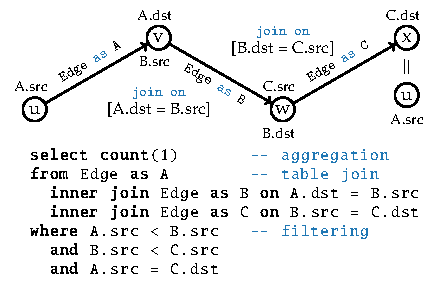
\includegraphics[width=0.65\textwidth]{figures/join-tc.pdf}
\caption{A graph query example of triangle counting using the standard SQL syntax.}
\label{fig:join-tc}
\vspace{-5pt}
\end{figure}

In comparison, we present a triangle counting program in the vertex-centric message passing model.
For each vertex $u$, we use $\mathit{Out}(u)$ to represent $u$'s outgoing adjacent list.
Then the algorithm consists of the following three supersteps.
\begin{itemize}
  \item \textbf{Step 1}:
    For each $v\in \mathit{Out}(u)$, vertex $u$ sends its own vertex id to $v$ if $u<v$;
  \item \textbf{Step 2}:
    Every vertex $v$ receives its incoming neighbors' vertex id from the message list, which is stored as a new list $\mathit{In}(v)$.
    Then for each $u\in \mathit{In}(v)$ and $w\in \mathit{Out}(v)$, vertex $v$ sends $u$ to $w$ if $v<w$;
  \item \textbf{Step 3}:
    Every vertex $w$ receives a list of vertex ids, which are the vertices that can reach $w$ in exactly two steps.
    Besides, each occurrence of $u$ in this list indicates a distinct path from $u$ to $w$.
    We store the list as $\mathit{In}^2(w)$.
    Then, for each $u\in \mathit{Out}(w)$, vertex $w$ counts the occurrence of $u$ in $\mathit{In}^2(w)$, and the sum is the number of triangles having $w$ as the largest vertex id.
\end{itemize}


The vertex-centric triangle counting algorithm is more complicated due to the explicit message passing in the algorithm description.
Also, we use $u,v,w$ to distinguish the role of the current vertex in each step to help readers understand the intended interactions.
However, this vertex-centric program and the SQL query in \autoref{fig:join-tc} has a close relationship, and using our language, we can derive this vertex-centric implementation from the graph query.
%Surprisingly, this vertex-centric program can be actually derived from a SQL query in \autoref{fig:join-tc}.

\begin{comment}
\subsection{Table Join v.s. List Comprehension}

Existing DSLs for Pregel programming uses parallel loop~\cite{green14} or list comprehension~\cite{palgol,fregel} to express the neighborhood communication.

, where users express how to associate the attributes of the graph (including vertex attributes, edge relations and global values, which are stored as separate tables) through inner joins, and then generate a new graph attribute through aggregation.
Compared to the vertex-centric model, it avoids the complexity of organizing the computation and communication,
but allow users to express the graph transformation through a more concise and descriptive relational query.
Then, the compiler cannot only compile the query into a parallel program, but also apply suitable optimizations by analyzing the communication patterns in the query.
%It XXX users from the issues like data placement, communication and optimizations.

We design a small query language for writing such graph queries, which combines the best features from both relational database and Pregel systems.
It uses the hash-based parallel query evaluation, its syntax supports iterative computation, and the compilation uses several graph-specific optimization techniques.


%\todo{how we address various issues using the knowledge in both sides (DB: distributed query evaluation, Palgol: iterative computation, Pregel: optimization techniques)}
%and XX features are to help writing graph applications or optimization.


%\todo{1. our method, its advantages and .. (maybe hard to understand)}
%which let users manipulates the graph data through table join and group by operations. It is sort of an enhancement of the list comprehension appeared in some domain-specific language~\cite{fregel,palgol,s6raph}.
\end{comment}


\subsection{An overview of SQL-core}

In this part, we present our language for writing graph computations in our proposed model.
%Although it is feasible to directly use SQL, its syntax better reflects the restrictions we made to our relational model (in \autoref{sec:detailed model}), and it also .
This language is in general similar to SQL, but its syntax is designed to reflect those restrictions we made on the computation model.
It is also a compositional language that allows users to easily perform the iteration over any kind of graph transformations.

%\subsection{Syntax}

The syntax of the language is defined in \autoref{fig:palgol-syntax}.
As described by the syntactic category \textit{trans}, a graph transformation contains a relational query following our high-level model, and the result table is bound to a variable.
Then, such graph transformations can be further composed or iterated %by two control structures called \textit{sequence} and \textit{iteration} (which are borrowed from Palgol~\cite{palgol}), 
as shown in the syntactic category \textit{prog}.
There are two kinds of iterations in our language, the \textit{for loop} and the \textit{fixed-point iteration}.
The former one iterates a program by a fixed number of rounds, and the latter one iterates a program until the specified table stabilizes.

The syntactic category \textit{query} defines the relational query in our language, which includes $Q_v$ for generating a vertex table and $Q_g$ for producing a global value.
Their differences are reflected in the \texttt{select} and \texttt{group by} clauses, while the table join and the filtering are the same.
%and has two forms $Q_v$ and $Q_g$ depending on what kind of table is generated.
%$Q_v$ generates a vertex table whose first column is alway vertex id and the second column is a value of a user-specified type, while $Q_g$ generates a global value containing a single value of a user-specified type.

%Here we use triangle counting (see \autoref{fig:join-tc}) as a running example to explain the special syntax for graph queries, in particular the table join in the \texttt{from} clause.
The syntax of table join is special in our language to better reflect the restrictions in our computation model.
We present two query examples in \autoref{fig:join-syntax}, which are part of the implementation of PageRank and triangle counting.
We first list all the vertices and their attributes used in a graph computation, then we assign a unique variable to each vertex and vertex attribute and connect then via link.
Each link is essentially a table specifying the relation between two variables.
In our language, we just put the tables after the keyword \texttt{from} to describe such graph computation.
%A graph computation is first represented as a graph pattern including all the vertices and their attributes relative to the computation.
%Then, for such a graph pattern, users assign a unique variable to each vertex and vertex attribute, and connect the variables via links, where each link is a table specifying the relation between the two variables.
%In our language, users just put the tables after the keyword \texttt{from} to represent a table join for that graph pattern.

A valid join then requires the variables and the links to form a spanning tree.
Remember that in our computation model, we require that for each join the two tables must have exactly one attribute in common.
Here, two links can join if they share an endpoint, and the join result is a connected subgraph.
Similarly, two connected subgraphs (intermediate join results) containing disjoint set of links can join if they share a node.
In both cases, the joint node automatically acts as the join attribute, so there is no need to explicitly specify the join attributes in our language.
We also note that, in our language, the order of tables does not matter, since deciding the join order is completely delegated to the compiler~(details in \autoref{sec:join-more}).

\begin{comment}
We present a inductive proof here.
For a tree with $n=1$ link, the only table representing the link is the join result.
Then, assume this statement holds for every $n=k$, then consider a connected tree with $n=k+1$ links, then we simply choose a leaf node and remove the link on this node.
The rest part of the tree is still connected and has $k$ links, so it has a valid join order, the removed link is a single table, and the two parts intersect on a single node.
\end{comment}

%We can even write {\texttt Edge(u,v)} $\Bowtie$ {\texttt Edge(w,x)} $\Bowtie$ {\texttt Edge(v,w)} although {\texttt Edge(u,v)} and {\texttt Edge(w,x)} should not be evaluated first, due to the lack of a common attribute.
%However, we do require that for any two vertices, there must exist a unique path between them.
%In such case, the graph pattern is a spanning tree, and the compiler can find a reasonable join order to evaluate the query.

The \texttt{where} clause contains the predicates to filter out the unwanted tuples in the join result.
Predicates are arithmetic expressions and comparison using only the columns in the join result, and we do not allow a predicate to contain any sub-query.
%More precisely, we hope to avoid the \textit{correlated} sub-queries where the evaluation of the sub-query inspects the values in the tuple of the parent query, in which case the query is hard to evaluate in parallel.
%By contract, a non-correlated sub-query can always be written as an individual query in our language.
Finally, the \texttt{select} clause generates either a vertex table or a global value.
We present both examples for $Q_v$ and $Q_g$ in \autoref{fig:join-syntax}.

%\newcommand{\hsp}[1]{\hspace{-3em}\hbox{#1}}
\begin{figure}[t]
\normalsize
\[
\begin{array}{lclr}
%\mathit{prog} & \Coloneqq & \mathit{decls}~\mathit{body} \\
%\mathit{decls} & \Coloneqq & \mathit{decl_1}~\ldots~\mathit{decl_k} \\
%\mathit{decl} & \Coloneqq & \mathtt{INPUT}~\mathit{sig}~\mathit{name} \\
\mathit{prog} & \Coloneqq & \mathit{trans}~|~\mathit{prog_1},\ldots,\mathit{prog_n}~|~\mathit{iter} \\
\mathit{trans} & \Coloneqq & \mathbf{set}~\mathit{name}:\mathit{sig}~=~\mathit{query} \\
\mathit{sig} & \Coloneqq & \mathbf{vertex\_table}~(\mathit{type})~|~\mathbf{global\_value}~(\mathit{type}) \\
\mathit{type} & \Coloneqq & \mathbf{vid}~|~\mathbf{int}~|~\mathbf{float} \\
\mathit{query} & \Coloneqq & \mathit{Q_v}~|~\mathit{Q_g} \\
\mathit{iter} & \Coloneqq & \mathbf{do}~\mathit{prog}~\mathbf{until}~\mathbf{fix}~(\mathit{name}) \\
 & | & \mathbf{for}~\mathit{var}~\mathbf{in}~\mathit{num}~\mathbf{to}~\mathit{num}~\mathbf{do}~\mathit{prog}~\mathbf{end} \\
\mathit{Q_{v}}  & \Coloneqq & \mathbf{select}~\mathit{var},~\mathit{column} \\
 & & \mathbf{from}~\mathit{table_1}~\mathbf{join}~\ldots~\mathbf{join}~\mathit{table_m} \\
 & & \mathbf{where}~\mathit{expr_1}~\mathbf{and}~\ldots~\mathbf{and}~\mathit{expr_r} \\
 & & \mathbf{group~by}~\mathit{var} \\
\mathit{Q_{g}}  & \Coloneqq & \mathbf{select}~\mathit{func}~(\mathit{expr}) \\
 & & \mathbf{from}~\mathit{table_1}~\mathbf{join}~\ldots~\mathbf{join}~\mathit{table_m} \\
 & & \mathbf{where}~\mathit{expr_1}~\mathbf{and}~\ldots~\mathbf{and}~\mathit{expr_r} \\
\mathit{table} & \Coloneqq & \mathit{name}~(\mathit{var}_1\ldots\mathit{var}_s) \\
\mathit{column} & \Coloneqq & \mathit{expr}~|~\mathit{func}~(\mathit{expr}) \\
\mathit{expr}  & \Coloneqq & \mathit{num}~|~\mathit{var}~|~\mathit{expr}~\mathit{op_b}~\mathit{expr}~|~\mathit{op_u}~\mathit{expr} \\
 & | & \mathbf{if}~(\mathit{expr})~\mathbf{then}~\mathit{expr}~\mathbf{else}~\mathit{expr} \\
\mathit{func} & \Coloneqq & \mathbf{max}~|~\mathbf{min}~|~\mathbf{count}~|~\mathbf{sum}~|~\mathbf{avg} \\
\end{array}
\]
\caption{The essential syntax of the query language.}
\label{fig:palgol-syntax}
\end{figure}

\begin{figure}
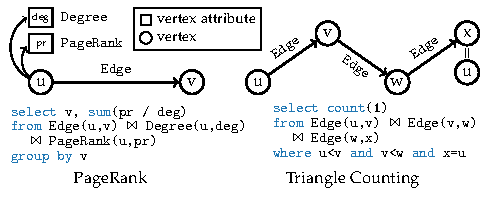
\includegraphics[width=0.9\textwidth]{figures/syntax-example.pdf}
\caption{Two query examples in our language.}
\label{fig:join-syntax}
\end{figure}

\subsection{Case studies}
\label{sec:algorithms}

\begin{figure}
PageRank
\begin{lstlisting}[language=sql-graph,frame=single]
for i in 1 to 30 do
  set Msg : vertex_table(float) =
    select v, sum(pr / deg)
    from Edge(u, v) join Pr(u, pr) join Deg(u, deg)
    group by v
  set Pr : vertex_table(float) =
    select u, 0.85 * msg + 0.15 / g
    from Msg(u, msg) join Size(g)
end
\end{lstlisting}
Single-Source Shortest Path
\begin{lstlisting}[language=sql-graph,frame=single]
do
  set Msg : vertex_table(int) =
    select v, min(du + len)
    from Edge(u, v, len) join Dist(u, du) join
         Dist(v, d)
    group by v
  set Dist : vertex_table(int) =
    select u, min(old, new)
    from Dist(u, old) join Msg(u, new)
until fix(Dist)
\end{lstlisting}
\caption{PageRank and single-source shortest path (SSSP) implemented in our language. The tables are assumed to be initialized.}
\label{fig:algorithms}
\vspace{-5pt}
\end{figure}

In \autoref{fig:algorithms} we implement the PageRank and single source shortest path (SSSP) using our language.
They are in general similar, so we just take PageRank as an example.
%Assuming that the input graph is already loaded as tables, 
A PageRank computation takes a fixed number of iterations, and in each round the vertex table \texttt{Pr(u,pr)} stores each vertex's tentative pagerank and is updated based on the previously computed result.
The other tables involved are the edge table \texttt{Edge(u,v)}, a vertex table \texttt{Degree(u,deg)} storing each vertex $u$'s out-degree, and a global value \texttt{Size(g)} storing the number of vertices in the graph.
The new pagerank for each vertex $v$ is calculated from all the tuples $(u, v, pr, deg, g)$ having the same $v$, by summing up the $pr / deg$ (to generate an intermediate table \texttt{Msg} in line 3) and then performing a local computation (in line 7 by a separate query) on each vertex.
%Here, \texttt{Msg} is an intermediate table that stores the temporary $pr / deg$ value for each $v$.
%This computation pattern is exactly the \textit{neighborhood communication} where a vertex inspects its surrounding vertices.

%We can even find more computation patterns in the other algorithms.
%For triangle counting, we join the edge table with itself to generate tuples $(u, v, w)$ such that $(u, v)$ and $(v, w)$ are edge relations.
%For the SV algorithm, we evaluate the joins of two vertex tables (line 9 and line 20), while the first join is nontrivial  that joined on the non-primary key of the first vertex table \texttt{D(u, du)}.

\begin{comment}
\begin{table}[t]
\centering
\caption{The APIs for our customized channels.}
\label{tab:basic-apis}
\begin{tabular}{l|p{5cm}|c|c|l}
\hline
\multirow{2}{*}{Channel} & \multirow{2}{*}{Description} & Use a & How many & \multirow{2}{*}{APIs} \\
& & Combiner? & supersteps & \\
\hline\hline
%\texttt{PeerToPeer<V>} &  & & \\
%& & & & \\
%\hline
\texttt{DirectMessage<K, V>} & Pregel's standard message channel. & \xmark & 1 & \texttt{send\_message(K dst, V val)} \\
& & & & \texttt{collect() -> pair<K, V>[]} \\
\hline
\texttt{CombinedMessage<K, V>} & Pregel's standard message channel using a & \cmark & 1 & \texttt{send\_message(K dst, V val)} \\
& combiner. & & & \texttt{collect() -> V[]} \\
\hline
\texttt{GroupBy<K, V>} & A local version of the \texttt{CombinedMessage} & \cmark & 0 & \texttt{send\_message(K dst, V val)} \\
& channel for local group by. & & & \texttt{collect() -> V[]} \\
\hline
\texttt{Aggregator<V>} & Pregel's standard channel for global com- & \cmark & 1 & \texttt{add\_message(V val)} \\
& munication. & & & \texttt{result() -> V} \\
\hline
\texttt{RequestRespond<K, V>} & A load balancing optimization for a com- & \xmark & 2 & \texttt{add\_request(int index, K dst)} \\
& mon communication pattern in Pregel & & & \texttt{respond(V[] values)} \\
& algorithms. & & & \texttt{collect() -> V[]} \\
\hline
\texttt{ScatterCombine<K, V>} & An optimization technique for the static & \cmark & 1 & \texttt{add\_edge(int index, K dst)} \\
& messaging pattern, which takes out redun- & & & \texttt{add\_message(int index, V val)} \\
& dant computation from a iteration.& & & \texttt{collect() -> V[]} \\
\hline
\multicolumn{5}{c}{\texttt{K}: the type of vertex id, \texttt{V}: the type of message value, \texttt{T[]}: a C++ vector with value type \texttt{T}.} \\
\end{tabular}
\end{table}
\end{comment}


\section{Compiling SQL-core to Pregel}
\label{sec:compilation}

In this section, we introduce our cost-based join algorithm for transforming a graph query to a query plan, which is the key step in our compilation.
The algorithm is generally based on the multiprocessor hash-based join algorithm~\cite{hashjoin-mp}, but
in the domain of graph processing, the following facts make our algorithm different from the previous work:
\begin{itemize}
\item
  Usually in graph computations, the join does not produce an exceedingly large intermediate table, making the memory consumption less a problem.
  Instead, we are more concerned with the communication cost. %in distributed-memory, and our algorithm uses a special cost model for deriving the most efficient query plan.
\item
  In distributed-memory graph processing, optimizations play an important role in achieving high-performance, therefore a straightforward join-based query evaluation may suffer various kinds of performance issues.
  This paper also focuses on extending the hash-join algorithm to make use of those optimizations.
  %\todo{todo}
  %However, those optimizations are explicitly applied in the user program, and several of them can only take effect in some particular scenarios.
  %To make use of these optimizations in our language, it is a challenge for the compiler to know when they are applicable.
  %\todo{cooperate with the optimizations}
 %Instead, we are more interested in using graph's property or communication patterns to improve the join, by using existing optimizations in graph-parallel system into our compiler.
\end{itemize}

%Next, we present the join algorithm and the special cost model for reducing communication cost.

We present the compilation algorithm in two parts.
The basic hash-join algorithm and our special cost model for communication cost are presented in this section, and the extension of our compilation algorithm for supporting various optimizations will be discussed in the next section.
The whole compilation also includes other steps like parsing and code generation, but they are either classic or  uninteresting, so we can safely skip them in this paper.

\subsection{Distribution of tables}
\label{sec:data-distr}

Processes are the basic computation unit in our graph system.
They share no memory, but can communicate with each other though the Message-Passing Interface (MPI).

Tables are horizontally partitioned across the processes in the system, and the partitioning is decided by a hash function and a column of the table.
The hash function maps a vertex id to a process id, then for each tuple, the hash value of the chosen column decides in which process it is stored.

The repartitioning of a table is a basic operation in our framework, which changes the hash column to another one.
When triggered, all the processes iterate over the tuples in the table stored on its local memory, and send each tuple to the designated process decided by the new column.


This table distribution strategy plays a central role in our compilation algorithm, which is the key to mapping our language to the vertex-centric execution model.
We justify our choice as follows:
%There are also some other options like distributing the tables by index or partitioning id, but our strategy has the following four advantages for our purpose:
\begin{itemize}
\item
  We can easily apply the multiprocessor version of the hash-based join algorithms~\cite{hashjoin-mp} to evaluate the query in parallel.
%\todo{need simplification}
  In particular, if both tables are partitioned by the join attribute, then all the tuples with the same join attribute (which is called a \textit{bucket}) will be stored on the same process, making the join operation efficient.
\item
  The hash-based partitioning strategy is similar to Pregel's design choice, which assigns vertices to machines based on a random hash.
  Having this connection, we manage to implement the query evaluation on Pregel, which avoids redundant work.
%\todo{need simplification}
  %Then, the join operation is independently performed in each bucket, and the repartitioning of the tables can be regarded as each bucket sending its tuples to other buckets.
  %, which is the key operation in our query evaluation,
  %In this sense, the query evaluation is also vertex-centric, and we can directly use Pregel to avoid redundant work.
\item
  The hash-based partitioning does not provide the best load balancing.
  However, it does not require any preprocessing, which is important to us since repartitioning may be frequently used in the query evaluation, especially for complex joins.
  %There are also other partitioning strategies like assigning a pre-calculated partitioning id for each vertex for better load balancing, but they require preprocessing and only work well when the join attribute .
  %Instead, repartitioning a table using hash function is much cheaper, which is suitable for dealing with complex joins.
\item
  There are already lots of optimizations developed for Pregel systems, and it is also our goal to automatically apply these optimizations in the query evaluation.
\end{itemize}

%\todo{check the necessity of the contents commented out}
\begin{comment}
In our graph system, tables are stored as C++ vectors.
Each process stores the list of vertices assigned to it in ascending order, so the vertex table is stored as a array of values associated to each vertex. 
The edge tables and intermediate join results are stored as an array of tuples sorted by the column they are partitioned by.
\end{comment}

\subsection{Inner join using vertex-centric computation}
\label{sec:join-two}

First, let us consider the join of two tables $T_1(a, b)$ and $T_2(a, c)$ having $a$ as the join attribute, which is the simplest case of join.
The communication cost of the join depends on the partitioning of the two tables:
\begin{itemize}
\item
  If both tables are partitioned by the join attribute $a$, then it is obvious that all the tuples with the same join attribute $a$ in both tables are on the same process.
  In this case, each bucket locally performs the join and introduces no communication cost.
  %The join result is a table partitioned by $a$.
\item
  Otherwise, suppose $T_1(a, b)$ is partitioned by $b$, then we perform a repartitioning on column $a$ by sending each tuple $(a, b)$ in $T_1$ to process $hash(a)$ through message passing.
 %The communication cost is the number of all tuples $(a, b)$ in $T_1$ satisfying $hash(a)\neq hash(b)$.
  We do the same thing for $T_2$ if it is not partitioned by $a$.
  Then we perform the local join.
\end{itemize}
%In the second case, the expected communication cost for $T$ is $size(T)*c$ where $c$ equals to $(w-1)/w$, assuming that the hash function uniformly distributes the tuples to all $w$ processes and column $a$ and $b$ are independent.

To clearly describe the compilation algorithm, it is helpful to syntactically distinguish a table's different ways of partitioning.
We introduce the following notation $T_1(a*, b)$ with an asterisk attached to one of the columns, representing the concrete data distribution of $T_1$ that is partitioned by column $a$.
Similarly, $T_1(a, b*)$ is $T_1$ partitioned by column $b$.
This notation also applies to the intermediate result of a join.
For example, we can say that the join result of $T_1(a*, b)$ and $T_2(a*, c)$ is a table $(a*, b, c)$.
Here, the order of the columns does not matter.
The join strategy described above is our \emph{default} strategy.

%In our implementation, all the tables are sorted by the column it is partitioned by, so the join operation simply uses the sort-merge join algorithm, and the result table is sorted by the join attribute.
%The repartitioning of a table is always followed by a sorting.
%For such table transformation, the communication cost is linear to the number of tuples in the result.

\begin{comment}
\subsubsection{The Join Operation}

In graph computation, we are intensively dealing with the vertex attributes.
As mentioned in \autoref{sec:representation}, vertex attributes are special tables that have the $id$ column as the primary key, so the join with other table can be computed very efficiently.
\end{comment}

\subsection{Efficient join ordering}
\label{sec:join-more}

When joining more than two tables, different join orders may result in different communication cost, and the decision of ordering is further affected by the subsequent computation.
%Moreover, for these different join results, there might be additional communication cost depending on the subsequent computation, which makes the decision of join order not trivial.
%When joining more than two tables, deciding the suitable join order is an important step in the query evaluation of a SQL-like language.
To see this, consider the following example that calculates the join of $T_1(a*, b)$, $T_2(b, c*)$ and $T_3(c*, d)$.
Two different query plans are presented in \autoref{fig:join-order}, where the left one joins $T_1$ and $T_2$ first, and the right one joins $T_2$ and $T_3$ first.
It should be noted that joining $T_1(a*, b)$ and $T_3(b, c*)$ is far too costly due to the absence of a common attribute, so we consider it as an invalid join.

\begin{figure}
\centering
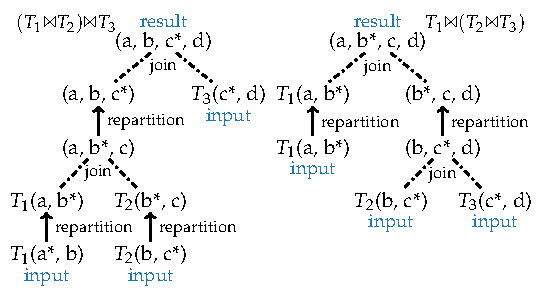
\includegraphics[width=0.8\textwidth]{figures/join-order.pdf}
\caption{Two different join orders to evaluate $T_1 \Bowtie T_2 \Bowtie T_3$.}
\label{fig:join-order}
\end{figure}

%As explained before, the communication cost is introduced by the repartitioning of the tables, and in \autoref{fig:join-order} 
We can see that the two query plans are likely to have different communication cost, since they use different number of repartition operations.
However, yet we cannot say that the second query plan is better than the first one or vice versa.
We should note that $(a, b, c*, d)$ and $(a, b*, c, d)$ are the same table partitioned by different columns.
Suppose the next join is on column $c$, then the second plan requires an additional repartitioning operation, which is not reflected in the current plan's cost.
Therefore, just considering the cost of table generation can lead to the sub-optimal problem.

To calculate the best join order in the presence of subsequent computation, the join algorithm should know in advance what column the solution is partitioned by.
Therefore, the input of the algorithm should is a pair $(S, x)$ where $S$ contains the tables to join, and $x$ is the column that the result table is partitioned by.
Here, $x$ should be an attribute of some $T\in S$, otherwise the input is not valid.
For example in \autoref{fig:join-order}, we say that the query plan on the left is a solution for $(\{T_1, T_2, T_3\}, c)$, and the query plan on the right is a solution for $(\{T_1, T_2, T_3\}, b)$.
%Which one is better depends on both the communication cost of the plan and how the subsequent computation use the result table.

\begin{algorithm}[t] % enter the algorithm environment
\caption{The cost-based join algorithm. \textbf{Input:} a set of tables $S$ and a column $x$ by which the result is partitioned. \textbf{Output:} a query plan with the minimum cost.}
\label{alg:solve}
\begin{algorithmic}[1]
  \State \Comment {Predefined join strategies}
  \State $\textit{strategies}\Leftarrow \{\textit{default},\textit{reqresp},\textit{static}~\}$
  \Procedure {Solve}{$S, x$}
  \State\Comment {Case 1: Dealing with one table.}
  \If{$|S|$=1}
    \State $T\Leftarrow$ the only table in $S$
    \State \Return $\textit{repartition\_if\_needed}(\texttt{Leaf}(T), x)$
  \EndIf
  \State\Comment {Case 2: Joining two tables.}
  \State $ret \Leftarrow \textit{null}$
    \For{$(S_l, S_r) \leftarrow \textit{valid\_split(S)}$}
      \For{$s\leftarrow \textit{strategies}$}
        \State $p \Leftarrow \textit{repartition\_if\_needed}($\Call{Join}{$s, S_l, S_r$}$,x)$
        \State\Comment {Cost estimation by \textit{cost()}}
        \If{$ret=\textit{null}$ \textbf{or} $\textit{cost}(p) < \textit{cost}(ret)$}
          \State $ret \Leftarrow p$
        \EndIf
      \EndFor
    \EndFor
    \State\Return $ret$
  \EndProcedure

  \State\Comment {The \emph{default} join operation on two tables}
  \Procedure {Join}{$\textit{default}, S_l, S_r$}
    \State $c \Leftarrow \textit{common\_attribute}(S_l, S_r)$
    \State $p_l \Leftarrow$ \Call{solve}{$S_l, c$}
    \State $p_r \Leftarrow$ \Call{solve}{$S_r, c$}
    \State \Return $\texttt{Join}(p_l, p_r, c)$
  \EndProcedure
\end{algorithmic}
\end{algorithm}

Given a query, let $S$ be the tables in the \texttt{from} clause and $xs$ be the columns appeared in $S$.
For every $x\in xs$, we find the best query plan for the input $(S, x)$ using \autoref{alg:solve}.
This is a top-down description of the hash-join algorithm, in which we solve a problem $(S, x)$ by breaking it into smaller sub-problems with the same structure.
It basically enumerates all possible query plans and selects the one with the minimum cost.
We leave the detailed explanation of the \textit{cost()} function in the next subsection.
To avoid redundant computation caused by solving the same problem repeatedly, we implement this algorithm in a bottom-up way using dynamic programming, ensuring that each $(S, x)$ is evaluated exactly once.
%Using the memoization technique is another practical option.

We made the algorithm extensible by predefining the join strategies in a global array in line 2.
The \emph{default} strategy is implemented in line 18, which is exactly the join algorithm introduced in \autoref{sec:join-two}.
Then, \autoref{alg:solve} with the default join strategy is sufficient to compile any table join to a valid query plan and then to a vertex-program, but yet we cannot ensure the high efficiency.
We will discuss the other join strategies in \autoref{sec:optimizations} for achieving better performance.
%The details of the \textit{cost()} function is presented in the next subsection, while the other auxiliary functions just do the jobs they literally mean.

\begin{comment}
\todo{todo: can delete}
This algorithm has an exponential time complexity.
For the join of $n$ tables, the number of all possible input is at most $2^{n}(n+1)$ where $2^n$ is the number of possible subset of $S$, and $n+1$ is the column by which the result is partitioned.
%The time complexity is $O(2^{2n}n)$ due to the enumeration of $S_l$ and $S_r$ for solving each sub-problem.
In practice, this complexity is totally acceptable, since for a graph computation, we seldom write a join having more than five tables.

%The space complexity is thus $O(2^{n}n^2)$ for storing the solutions for all possible inputs, where the additional factor $n$ is the size of query plan.
\end{comment}

\subsection{Cost estimation}
\label{sec:cost}

\begin{table}[t]
\centering
\caption{The estimation of the communication cost and the table size for each type of node in the query plan.}
\label{tab:cost-estimation}
\begin{tabular}{lll}
\hline
node $t$ & $cost(t)$ & $size(t)$ \\
\hline
$\texttt{Leaf}(t_1)$ & 0 & $n$ or $m$ \\
$\texttt{Repar}(t_1)$ & $\mathit{size}(t_1)*(w-1)/w$ & $\mathit{size}(t_1)$ \\
$\texttt{Join}(t_1,t_2)$ & $\mathit{cost}(t_1)+\mathit{cost}(t_2)$ & $\mathit{size}(t_1)*\mathit{size}(t_2)/n$ \\
\hline
$\texttt{ReqResp}(t_1,t_2)$ & $n*(1-e^{-\mathit{size}(t_1)/n})+$ & $\mathit{size}(t_1)$ \\
& $\mathit{cost}(t_1)+\mathit{cost}(t_2)$ & \\
\hline
\end{tabular}
\end{table}

In this part, we present the implementation of \textit{cost()} to complete the \autoref{alg:solve}.
The query plan has a tree structure where each leaf node is an input table and an internal node represents a result table of a repartitioning or a join (see \autoref{fig:join-order} as an example).
Our \textit{cost()} function applies to a node in the query plan and returns the communication cost to generate the result table.
%Our cost function applies to a tree node and returns the following information for the current table: the communication cost (in terms of bytes) to generate this table, the record size (in terms of bytes) and the estimated number of rows.
%For simplicity, this function is a structural recursion that only looks at the type of the current node and the estimated cost of its direct children.
We also need an auxiliary function \textit{size()} defined in the same way returning the estimated table size.

Three parameters $n$, $m$ and $w$ are used by our \textit{cost()} and \textit{size()} function, which represent the number of vertices and edges in the input graph and the number of processes launched by the user.
One can also use the density ($m/n$) to implement these functions, and $w$ can be safely replaced by a large enough value.
The two functions are defined in \autoref{tab:cost-estimation} for each type of node in the query plan.
To obtain a more precise communication cost, we also keep track of the record size of each table (see \autoref{sec:filtering}), but it is orthogonal to the implementation of these two functions.

\begin{comment}
\todo{TODO: need to simplify}
\begin{itemize}
\item \textbf{leaf node}:
  A leaf node in the query plan is an input table, which is initially partitioned by one of its attributes.
  Directly referring to an input table does not incur any communication cost.
  The table size (number of rows) depends on the type of the table, which is $n$ for a vertex table (or a vertex set) and $m$ for an edge table.
 %There is no communication cost when directly referring to such tables, and the table size is $n$ and $m$ respectively.
\item \textbf{repartition node}:
 A repartition node changes the data distribution of a table (the only child), so the table size remains the same.
 Suppose $u$ and $v$ are the hash columns before/after the repartitioning, then the communication cost is the number of rows $(u, v, \ldots)$ having $hash(u)\neq hash(v)$ multiplied by the record size.
 Here, we assume that column $u$ and $v$ are independent, then the expected number of rows to be transmitted is $s*(w-1)/w$, where $s$ is the size of the table.
\item \textbf{join node}:
 A join node in the query plan joins two tables using our \textit{default} strategy.
 There is no communication cost for the join operation, and we just sum up the communication cost of the subtrees.
 For the table size, we simply use $s_1*s_2/n$ as an estimation where $s_1$ and $s_2$ are the size of each table.
\end{itemize}
\end{comment}

\subsection{Result table generation}

%Up to now, we have discussed the evaluation of the join over a sequence of tables.
Next, we briefly go through the result table generation, which transforms the join result to either a vertex table or a global value depending on the syntax (see $Q_v$ or $Q_g$ in \autoref{fig:palgol-syntax}).

\subsubsection{Vertex Table}
\label{sec:vertex-table-gen}

A vertex table is generated from the join result via the \textit{group by} operation over one of the columns in the table.
The vertex attribute is calculated from an aggregate function.
The following query from PageRank shows a typical example of vertex table generation:
\begin{lstlisting}[language=sql-graph]
select v, sum(pr / deg)
from Edge(u, v) join Pr(u, pr) join Deg(u, deg)
group by v
\end{lstlisting}

The vertex table having $v$ as the first column is generated from the join result $(\mathit{u},\mathit{v}*,\mathit{deg},\mathit{pr})$.
For each row, we first compute the expression inside the aggregation function (which is $pr/deg$ in this example),
then all the rows with the same attribute $v$ sum up their values of $pr/deg$, generating a single value $sum(pr/deg)$ associated to vertex $v$.
Those $v$'s that have not appeared in the join result are assigned with the default value $0$.
%The vertex table generation only involves local computation.

%For simplicity, we estimate the communication cost as $n(w-1)(1-(1-1/w)^{s/n})$~according to this work~\cite{balanced} by assuming a uniform degree distribution, where $s$ is the size of the join result.

%Note that, the aggregation function S is optional, since it is possible that the join result is grouped by a primary key.

%The syntactic category for generating the vertex table is $Q_v$ in \autoref{fig:palgol-syntax}, which performs a \texttt{group by} over one of the columns in the join table, with an aggregate function to generate a vertex attributes.
%The complete algorithm is shown below.
%Suppose the join is performed over a list of tables $S$ and $x$ is the column to be grouped by, we enumerate every attribute $c$ and calculate a query plan for the input $(S, c)$ using \autoref{alg:solve}.
%Each query plan has its own communication cost, and the whole cost of generating a vertex table should also include the cost of the \texttt{group by} operation over the join result.
%We the choose the query plan with the minimum total communication cost.

%The generation of a vertex table contains the repartitioning of the join result (suppose $c\neq x$) and the group by operation.
%We can actually combine the repartitioning and the group by operation together to reduce the communication cost, by directly using Pregel's \texttt{CombinedMessage} channel.

\subsubsection{Global Value}

The generation of a global value from the join result is simply implemented by all the processes performing an \textit{all-reduce} operation using MPI.
In such case, the actual data distribution of the join result does not matter,
therefore we enumerate every column $c$ and choose the query plan $(S, c)$ having the minimum communication cost.

%much simpler, by each row evaluating the \textit{expr} inside the aggregate function (see \autoref{fig:palgol-syntax}) and then all the processes performing an \textit{all-reduce} operation.
%On a Pregel system, such global communication is implemented by the \texttt{Aggregator} channel, and the communication cost of this channel can be neglected.
%The join result is chosen in this way: we enumerate every attribute $c$ and simply pick the query plan $(S, c)$ having the minimum communication cost.

%In \autoref{fig:palgol-syntax}, $Q_g$ is the syntactic category for generating global value.
%For each tuple in the join result, the query evaluates an expression \textit{expr} and uses an aggregate function to combine the \textit{expr} to a final result.
%This is simply implemented by each process's local aggregation followed by a reduce operation.

\begin{comment}
\subsection{Code Generation}

The last part of the compilation is the transformation from each query plan to a sequence of supersteps, which is relatively simple.
The generation of supersteps is implemented by a single pass of the query plan, where on each node, we:
\begin{itemize}
  \item decide in which superstep the current table is evaluated, which is calculated by a topological sorting;
  \item generate the code for producing the current table (a reference to a vertex/edge table or a join operation);
  \item update the association between the variables and the columns in the current table.
\end{itemize}
The result of a single query is a sequence of supersteps connected by message passing, and such data structure is further fed to the \textit{sequencing} and \textit{iteration} operations, resulting in a complete program consisting of both supersteps (states with local computation code) and control flow (state transitions).
This technique is already studied in the Palgol language~\cite{palgol}, and interested readers can refer to the original paper for more details.
\end{comment}


\section{Deep optimizations for SQL-core}

In this section, we present various strategies for optimizing the query plan for reducing the computation and communication cost.
Our language not only applies several standard optimizations studied in relational database, but also makes use of graph-specific optimizations in the graph system.
We show that our relational model provides abundant hints for the compiler to optimize different kinds of graph transformations.
 %which leads to significant performance gain compared to a standard implementation.
%Moreover, such decision procedure can be easily integrated into our cost-based join algorithm.
%We therefore extends the compilation algorithm in \autoref{sec:compilation} to detect the feasibility of using these optimizations and generates more efficient programs for users.

\subsection{Filtering the table entries}
\label{sec:filtering}

The query filters perform a straightforward task --- filtering the rows and columns of a table --- to reduce the size of intermediate tables as well as the communication cost.
The technique is intuitive and standard: rows are eliminated based on the predicates, and columns are removed when they are not used in the consequent computation.
We push down the filters as early as possible.
We also extend our cost-based join with an additional attribute, the record size, to estimate the communication more precisely.
%We extend our cost-based join algorithm, mainly the cost function defined in \autoref{sec:cost}, to support the query filtering.

\begin{comment}
The cost function applies to a subtree in the query plan and returns the communication cost and the size of the result table.
We add an additional parameter $S$ to the cost function, which is the set of input tables involved in the join.
Suppose the number of predicates that are applicable to the join result of $S$ is $k$, then for each predicate, we reduce the estimated table size by a factor $a (0<a<1)$. %, making the number of rows to be $\Pi_{t\in S} size(t)*a^k/{n^{|S|-1}}$.
The unused columns can be easily recognized by the consequent computation and the remaining predicates, and the record size is calculated accordingly.
Both $k$ and the record size can be preprocessed for each $S$, so the time consumption for compilation is negligible.
%, we select the unused predicates from the \texttt{where} clause that are applicable to the current table, and filter the rows instantly.
%For each predicate applied here, we reduce the estimated table size by a factor $a (0<a<1)$, and the predicate is marked used.
%After that, the unused columns are recognized (which are the ones not appeared in the current node's ancestors and the remaining predicates), and the record size is recalculated accordingly.
%Note that for each node in the query plan, which is itself a solution for some input $(S, x)$, the rows and columns to remove can be totally decided by the set of tables $S$

\end{comment}

\subsection{Improved vertex-table generation}

%In distributed graph algorithms, it is common that a vertex table is generated by a \textit{group by} operation over the join result using an aggregation function, as shown in \autoref{fig:algorithms}.
In \autoref{sec:vertex-table-gen}, the generation of a vertex table consists of two steps: (1) obtain the join result partitioned by the vertex table's first column, and (2) perform a local \textit{group by} on that column.
In many cases, for example calculating the \texttt{Msg} table for PageRank and SSSP in \autoref{fig:algorithms}, the query plan in the first step ends with a repartitioning operation.
Repartitioning is a relatively communication-intensive operation, since most rows in the join result are involved.
However, when the next operation is \textit{group by}, we can reduce the communication cost by shrinking the table before partitioning.
%It simply uses the associativity of the aggregation function.

%To implement this optimization, we do not change the join algorithm but only modify the table generation.
Our improved vertex-table generation consists of the following three steps: (1) obtain the join result partitioned by some column $c$; (2) each process groups the tuples on its local memory by column $c$ and then repartition the join result by the vertex table's first column $v$, and (3) perform a second \textit{group by} operation on $v$.
It generates the same table due to the associativity of the aggregation function.
In the new algorithm, we need to enumerate $c$ and select the one that minimizes the total communication cost.
\autoref{alg:solve} estimates the cost of the first step, and the cost of the second step can be estimated by $n(w-1)(1-(1-1/w)^{s/n})$ by assuming a uniform degree distribution~\cite{balanced}, where $s$ is the size of the join result.

%\subsection{ Tables}

%Most distributed graph computations are iterative, therefore the 

%\subsection{Graph-specific optimization}

%In this part, we present two case studies to show how we detect and use existing optimizations to improve the query evaluation.
%Then, as mentioned, our compilation algorithm is designed with extensibility, so the detection of these cases can be implemented as new \texttt{join strategies} so that they can perfectly work with our cost-based join algorithm.

%Let us consider a vertex-centric algorithm presented in \autoref{algo:req}, which for each vertex $u$ in a tree computes the grandparent (current parent's parent) vertex.
%Each vertex $u$ initially holds a pointer to its parent vertex, while the root vertex points to itself.

\subsection{Introduction of the optimized channels}
\label{sec:optimizations}

In the last part, extend our compiling algorithm to support optimization channels.

\subsubsection{The request-respond channel}

Several graph algorithms (like Shiloach-Vishkin~\cite{ShVi82} and LACC~\cite{lacc}) may use an auxiliary structure called \emph{pointer graph} to keep track of the connectivity information during the computation.
The pointer graph is essentially a forest of rooted trees consisting of all the vertices in the input graph.
To store this structure, each vertex just maintains a field indicating its current parent vertex in the pointer graph (a root vertex points to itself), and communication occurs between a vertex with its parent or children.
A common operation on this data structure is to find the grandparent for every vertex, which is known to have skewed communication pattern.

% and such structure can be obviously stored as a vertex table in our model.

We describe this operation in our language.
The pointer graph can be represented by a vertex table \texttt{P(id, parent)}, and each vertex's grandparent is also a vertex table \texttt{GP(id, grandparent)}.
The following query generates the grandparent table from the parent table:
\begin{lstlisting}[language=sql-graph]
  select u, w
  from P(u, v) join P(v, w)
  group by u
\end{lstlisting}
The default join strategy converts $P(u*,v)$ to $P(u,v*)$ and performs a local join on column $v$, obtaining $(u,v*,w)$.
Then, another repartitioning is required to generate the result table $(u*,w)$.
In a vertex-centric view, each vertex $u$ sends a message to its parent $v$ in the first repartitioning, and every parent vertex $v$ replies to its children the $w$ in the second one.
They are exactly the \emph{request} and \emph{respond} steps.

In practice, there are high-degree parent vertices $v$ due to the algorithm logic, causing an imbalanced distribution for $P(u, v*)$.
One solution proposed for this issue is the request-respond paradigm~\cite{yan2015effective}.
After all the vertices emit the requests, the processes will first merge the requests to the same parent vertex and then send out only the distinct requests.
As a result, a high-degree parent can receive at most one request from each process instead of one request from each of its children, which effectively avoid the hot spot.
%In this plan, the tuple $(u, v)\in D$ is first sent to $hash(v)$ and then sent back, while $u$ is not directly involved in

%A detailed explanation of this optimization is presented in the right part of \autoref{fig:req-plan}.
%Since the join attribute $v$ is the primary key of $D(v, w)$, we can consider $D(v, w)$ as a function $f(v)\rightarrow w$, and the join simply applies $f$ to each $v$ in the other table $D(u*, v)$.
%The new plan is to generate a partial function $f(v)\rightarrow w$ for process that only applies to those $v$'s appeared in $D(u*, v)$.
%Therefore, each process $p$ calculates the domain of $f'$ as a new relation $R(p,v)$ (which is in practice much smaller than $D(u,v)$) and sends $R(p,v) to \Bowtie D(v,w)$, which is more message-efficient than using $D(u*,v)$ in the original plan.

%Here we clarify the conditions for applying this optimization.
The detection of this optimization is achieved by extending \autoref{alg:solve} with a new join strategy \textit{reqresp} and adding a new \texttt{ReqResp}$(t_1,t_2)$ node in the query plan.
An auxiliary function \textit{is\_primary\_key()} is used to decide whether a column in the table is the primary key.

\begin{algorithm}[t] % enter the algorithm environment
\caption{The \textit{reqresp} join strategy. \textbf{Input:} two sub-queries $S_1$ and $S_2$ to join. \textbf{Output:} a request-respond query plan or \textit{null} if not applicable.}
\label{alg:solve2} % and a label for \ref{} commands later in the document
\begin{algorithmic} % enter the algorithmic environment
  \State\Comment {The \emph{reqresp} join operation on two tables}
  \Procedure {Join}{$\textit{reqresp}, S_l, S_r$}
    \State $c \Leftarrow \textit{common\_attribute}(S_l, S_r)$
    \If{$\textit{is\_primary\_key}(S_r, c)$}
      \For{$u \leftarrow \textit{all\_attributes(S)}$}
        \State $p_l \Leftarrow$ \Call{solve}{$S_l, u$}
        \State $p_r \Leftarrow$ \Call{solve}{$S_r, c$}
        \State \Return $\texttt{ReqResp}(p_l, p_r, u)$
      \EndFor
    \EndIf
    \State\Return $\textit{null}$
  \EndProcedure
\end{algorithmic}
\end{algorithm}

The detailed implementation of this strategy is in \autoref{alg:solve2}, and the communication cost is presented in \autoref{tab:cost-estimation} under the assumption that attribute $u$ and $v$ are independent. %, which is $n*(1-e^{-s/n})$ where $s$ is the table size of $T_2$.
Note that the cost function for default join does not tell anything about the load balancing, but \texttt{ReqResp} plan is generally preferable when it is applicable.


\begin{comment}
by tables to be join.
We list all the conditions that are required to be satisfied by this optimization:
\begin{itemize}
  \item A table $T_1(v*,\ldots)$ having the join attribute $v$ as the primary key;
  \item The other table $T_2(u*,\ldots)$ partitioned by an attribute $u$ other than $v$;
  \item The join result partitioned by $u$.
\end{itemize}
We add a special node in the query plan (in the lower-left part of \autoref{fig:req-plan}) as the output of a successful the detection, and it compiles to the request-respond channel (shown in \autoref{tab:basic-apis}) in the code generation phase.

In this query, the join result is partitioned by $u$, which is the same as one operant $D(u*, v)$, and the join attribute $v$ happens to be the primary key of the other operant $D(v*, w)$, and the .
%It is called the request-respond paradigm in Pregel, since it is a two-round communication pattern where every vertex $u$ first sends a request to $v$ for each $(u, v)\in D$, then receives $v$'s attribute $w$ in the next round.
\end{comment}


\subsubsection{The scatter-combine channel}

%is a common strategy that the repeated computation can be taken out of the loop instead of being computed on the fly.
Scalable graph computations are usually iterative, and it is a natural idea to take out repeated computation from the iteration.
Let us consider the following example, which is an iterative program that calculates the join of a vertex table $Value(v, w)$ and an edge table $Edge(u, v)$ in every iteration.

\begin{lstlisting}[language=sql-graph]
do
  set T : vertex_table(int) =
    select u, min(w)
    from Edge(u, v) join Value(v, w)
    group by u
  ...
until fix(..)
\end{lstlisting}

At first glance, it is a request-respond pattern where each $u$ sends a request to every neighbor and calculates the minimum response value.
However, the real issue is not the load balancing but the heavy computation inside the iteration.
In this query, the edge table $Edge(u, v)$ is immutable and there is no filter, meaning that we will send the vertex $v$'s current value $w$ to every neighbor of $u$ in every iteration.
A graph computation that frequently sends vertex attributes along a fixed set of edges is said to have the static messaging pattern~\cite{zhang2019composing}.
A conventional implementation incurs heavy computational cost due to the sorting of the large message list, while the solution they proposed is organizing the edges in a particular order, so that the message passing can be implemented in a linear scan.

The requirements of this optimization is stricter than the request-respond pattern.
The query should (1) be inside an iteration, (2) have the edge table $\texttt{Edge}(u,v)$ in the join, (3) have no filter applicable to the current join, and (4) have $u$ as the first column and some value associated on $v$ as the second column, or vice versa.
Each step can be easily detected by an auxiliary function, and due to the page limit, we do not present the detailed implementation in this paper.

\begin{comment}
To see this problem clearly, we present the standard plan for this query in the left side of \autoref{fig:scatter-plan} with details of message processing.
We first compute the join of the two tables and get the intermediate result $(u, v*, w)$.
By using Pregel's combiner mechanism, for each tuple $(u, v, w)$ we send the message value $w$ to vertex $u$, but before that a single $w'$ is computed for each unique $u$ representing the minimum message value.
This is equivalent to a local group by on table $(u, v*, w)$.

Considering that the query is inside an iteration, the transformation from $E(u*, v)$ to $E(u, v*)$ should be put outside the iteration, since the table $E(u, v)$ is immutable.
Second, to combine the messages, we need to sort the table $(u, v*, w)$ in each iteration on column $u$ (which by default is sorted by $v$).
However, we should note that for the join result $(u, v*, w)$, only the column $w$ is different in each round, meaning that the sorting can be also taken out of the iteration.
This is the essential idea of scatter-combine optimization~\cite{zhang2019composing}.

We put the optimized plan in the right side of \autoref{fig:scatter-plan}, where an intermediate table $E'(u, v)$ is actually used in the computation.
Such $E'(u, v*)$ is just a simple transformation from the original table $E(u, v)$..
We compute $E'(u, v*)$ outside the iteration,
\begin{comment}

\end{comment}

\begin{comment}
\subsection{Graph-Specific Optimizations}

The communication pattern is an important aspect in distributed graph algorithms, which gives a high-level way of reasoning about the interactions between vertices.
Moreover, in some Pregel systems~\cite{channel,pregelplus}, it also plays the central role in optimization, where a proper implementation of a communication pattern can lead to a dramatic improvement on the performance.

For example, some algorithms require a vertex sending a value to all its outgoing neighbors , whereas some algorithms require reading values from incoming values.
Essentially, a communication pattern \textit{push} or \textit{pull} operation over a specific set of vertices.
In general, these data access patterns can be classified into two categories: push and pull.

The \textit{push} operation is just sending a message, while a \textit{pull} operation fetches data from other vertices.
In some scenarios, push and pull are just different perspectives of describing the same algorithm.
For example, Pregel's PageRank algorithm~\cite{pregel} is expressed by each vertex sending along its outgoing edges the tentative PageRank value divided by the number of outgoing edges.
Alternatively, it can be also described by every vertex pulling the PageRank value from its incoming neighbors~\cite{fregel,palgol}.
\end{comment}

\section{Evaluation of SQL-core}
\begin{table}[t]
\centering
\caption{Graph datasets used to evaluate our framework.}
\vspace{-5pt}
%\footnotesize
\label{tab:datasets}
\resizebox{\columnwidth}{!}{
\begin{tabular}{lrrrl}
\hline
Graph & Vertices & Edges & Density & Description \\
\hline
DBpedia & 18.27M & 136.54M & 7.47 & The DBpedia hyperlink graph~\cite{konect} \\
Queen\_4147 & 4.15M & 166.82M & 40.23 & 3D structural problem~\cite{davis2011university} \\
HV15R & 2.02M & 283.07M & 140.33 & Computational Fluid Dynamics Problem~\cite{davis2011university} \\
uk-2005 & 39.45M & 936.36M & 23.73 & 2005 web crawl of .uk domain~\cite{davis2011university} \\
twitter7 & 41.65M & 1.47B & 35.25 & twitter follower network~\cite{davis2011university} \\
sk-2005 & 50.64M & 1.95B & 38.50 & 2005 web crawl of .sk domain~\cite{davis2011university} \\
\hline
\end{tabular}
}
\end{table}

In this section, we evaluate the performance of our generated code, and also compares our system with other frameworks.
We select four representative algorithms in our evaluation, including PageRank (PR)~\cite{google,pregel}, Shiloach-Vishkin algorithm (SV)~\cite{ShVi82,yan2015effective}, Triangle Counting (TC) and Single-Source Shortest Path (SSSP)~\cite{pregel}.
The experiments are conducted on Amazon EC2 cluster of 16 nodes (with instance type r4.2xlarge), each having 8 vGPUs and 61 memory size.
%The bandwidth between any two nodes is 10Gb.
We use 128 processes (single-threaded) in our evaluation, and the datasets are listed in \autoref{tab:datasets} using real-world graphs.

\subsection{Performance without optimizations}

\begin{figure}
\centering
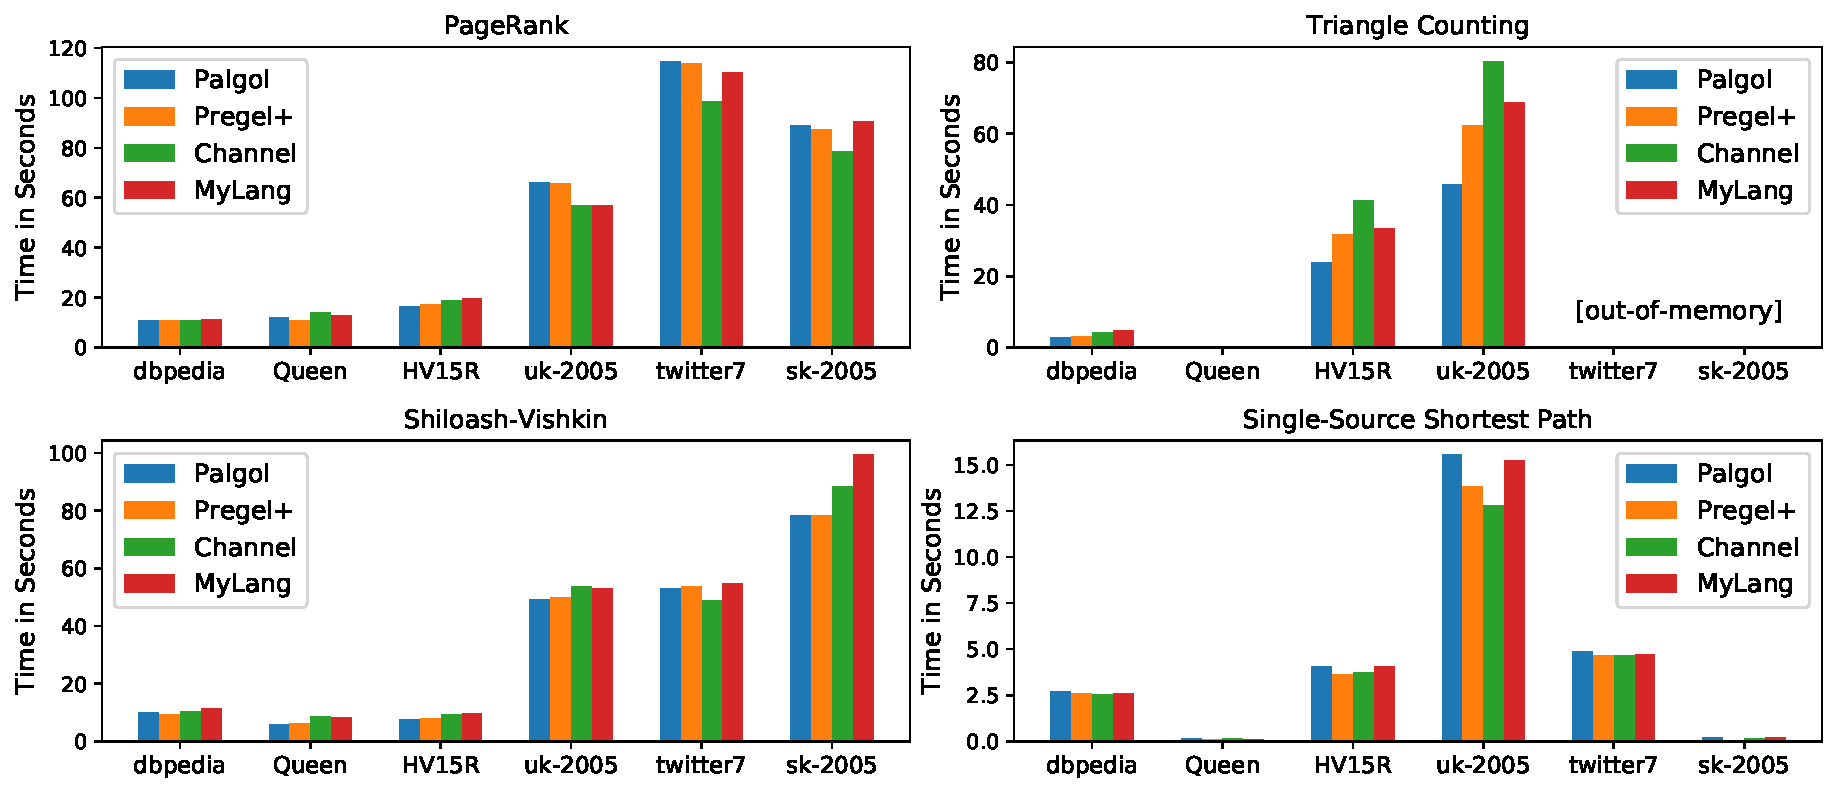
\includegraphics[width=\textwidth]{figures/performance.pdf}
\caption{Performance of the unoptimized vertex-centric programs in various systems.}
\label{fig:performance}
\end{figure}

We first evaluate the performance of our generated program using only Pregel's standard message passing interface.
The main competitors are listed below:
\begin{itemize}
  \item \textbf{Palgol}: a vertex-centric DSL on top of Pregel+~\cite{yan2015effective}.
  \item \textbf{Pregel+}: the Pregel+ framework with the implementations of various Pregel algorithms by human.
  \item \textbf{SQL-core}: our DSL that compiles to the Pregel-channel system (see \autoref{chap:vcgp}).
  \item \textbf{Channel}: the original Pregel-channel framework with two additional optimizations~(introduced in \autoref{sec:optimizations} but not used in the current experiment).
  %Graph algorithms are carefully optimized using the proper combination of optimizations.
\end{itemize}
All of these systems are implemented in C++ as a group of headers.
There are also other DSLs for Pregel implemented on other systems, like Green-Marl~\cite{green14} that generates C++ code and Fregel~\cite{fregel} with the Giraph~\cite{giraph} back end.
We choose Palgol due to its expressive power for practical Pregel algorithm and its concrete implementation for efficiency.

The results are presented in \autoref{fig:performance}.
On all the six graphs, we observed similar runtime for the four programs.
Our language did generate the plan with the least message size, which makes our program comparable with human written code (Pregel+ and Channel).
The Palgol language also generates the code with optimal messages size.
These systems have subtle differences in implementation, like the choice of MPI function, serialization methods and so on, making the runtime differs a bit.

This experiment mainly reveals the performance characteristics of the back end system.
In fact, our language is possible to be compiled to any of these back ends, but we choose the current system mainly due to the powerful optimizations it supports, which will be presented in the next subsection.

\begin{figure}
\centering
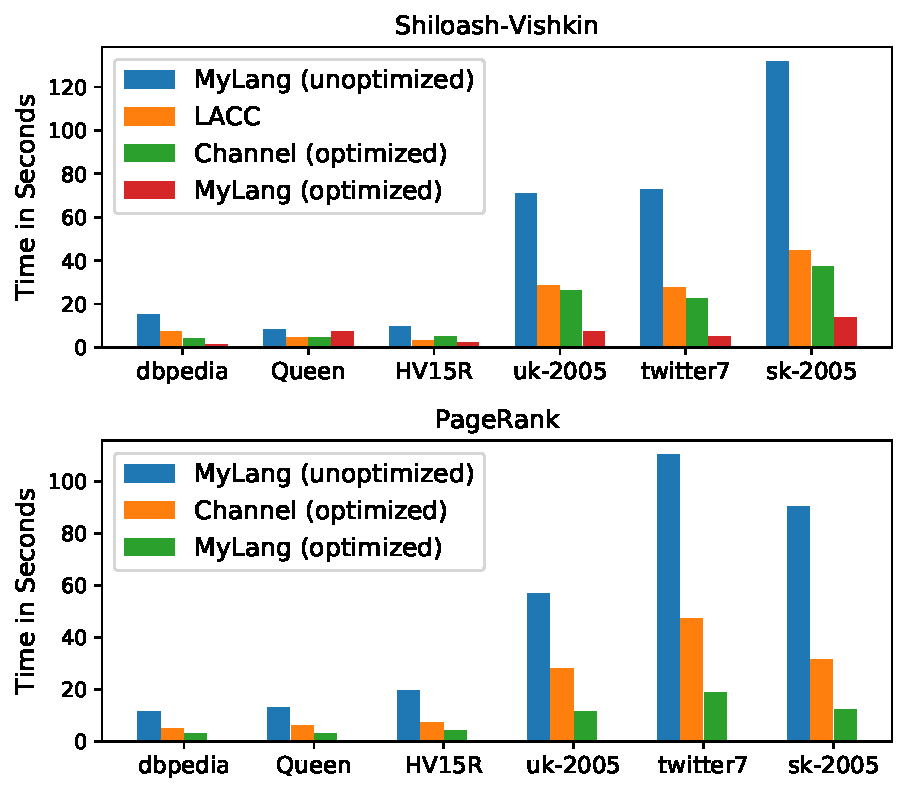
\includegraphics[width=0.8\textwidth]{figures/both.pdf}
\caption{Performance of the Shiloach-Vishikin and PageRank algorithm in various systems. Both algorithm requires the optimization techniques introduced in \autoref{sec:optimizations}. }
\label{fig:sv-results}
\end{figure}


%For triangle counting, the Pregel+ programs
\begin{comment}
\subsubsection{Message size}
First, for all these five algorithms, the message consumption of our language is the least, and is the same as the hand-written code on pregel-channel, meaning that our computation model and compilation algorithm does not introduce unnecessary data communication.
This is important, which shows that a SQL-based language can be transformed to a message-efficient vertex-centric implementation.
Both of Palgol and Pregel+ consume remarkably more message for SV, which is up to 4x message size compared with the optimal one.
However, this is due to Pregel+'s monolithic message passing interface~\cite{zhang2019composing} that cannot efficiently deal with multiple communication in the same program.

\subsubsection{Execution time}
Regarding to the execution time, the compiler-generated code is in general as efficient as the human written ones on Pregel-channel for most algorithms, except for SSSP that suffers a $142\%$ slowdown.
The main reason is that Pregel's execution logic, especially the \textit{voting to halt} mechanism to deactivate converged vertex during computation, can greatly accelerate the execution of SSSP.
We observed that, only a very small portion of the vertices are active during the SSSP computation.
Instead, both Palgol and our language execute a state transition machine inside the loop, which introduce a significant computational overhead.
Moreover, our language scan the vertex tables for multiple times inside a loop, resulting in a little bit more execution time compared to Palgol.

%For triangle counting, we found that the join of two edge tables introduces additional cost, which is in general slower than each vertex joining two local list.

For the other graph algorithms, the difference on execution time is not significant.
It is slightly faster on PageRank (less than $1\%$), and is $10\%$ to $20\%$ slower on SV and WCC.
Difference from the message size which is completely decided by the compilation algorithm, there are far more reasons that can affect the execution time, like the quality of the code generation, the use of peephole optimizations, the data structure and so on.
For these algorithms, we can only conclude here that the performance gap is not significant, and there are still room for us to further improve the compiler implementation.
Compared to Palgol/Pregel+, our language is as efficient for PageRank and WCC, and is up to 2.25x faster for SV due to Pregel+'s monolithic message passing interface, as mentioned before.
\end{comment}


%We next evaluate the performance of generated code using the optimizations introduced in \autoref{sec:optimizations}.
%In this evaluation, we only user the PageRank and the SV algorithm, which can be optimized by the underlying system's optimizations.
%We compare our language with the hand-written code only, since existing DSLs do not support any graph-specific optimizations.

\begin{comment}
\centering
\caption{Optimizations Used/Detected in Implementations}
\label{tab:detect}
\begin{tabular}{c|c|c|c}
\hline
Algorithm & Program & Request-Respond & Scatter-Combine \\
\hline
\multirow{2}{*}{PageRank}
 & Channel+opt & & \cmark \\
\cline{2-4}
 & MyLang+opt & & \cmark \\
\hline
\multirow{2}{*}{SV}
 & Channel+opt & \cmark & \cmark \\
\cline{2-4}
 & MyLang+opt & \cmark & \cmark \\
\hline
\end{tabular}
\end{comment}

\subsection{Performance with detected optimization}

In this section, we focus on the SV and PageRank algorithm, which requires the optimization techniques presented in \autoref{sec:optimizations} to achieve high efficiency.
The evaluation results are presented in \autoref{fig:sv-results}.

The SV algorithm uses both optimizations and is presented in the upper-part, including the unoptimized SV using our default join strategy (leftmost), and the optimized SV with both optimization techniques detected (rightmost).
The original channel-based Pregel system also has these two optimizations, so we include it in the figure. 
We further include the linear algebra connected component (LACC)~\cite{lacc} algorithm here, the state-of-the-art scalable algorithm for finding connected components.

The compiler successfully detects the two optimizations.
Compared to our unoptimized version, our optimized SV gains a huge speedup from 1.14$\times$ to 14.29$\times$ on all the six datasets, and compared to the original \emph{Channel} implementation, this number is on average 2.7$\times$ (max 4.44$\times$).
For PageRank, we also observe a significant performance gain compared to unoptimized version (avg. 5.21$\times$, max 7.45$\times$), and it is faster than the PageRank in the original \textit{Channel} system.

\section{Related work}

Google's Pregel \cite{pregel} proposed the vertex-centric computing paradigm, which allows programmers to think naturally like a vertex when designing distributed graph algorithms.
Some graph-centric (or block-centric) systems like Giraph\plus\cite{thinkgraph} and Blogel~\cite{yan2014blogel} extends Pregel's vertex-centric approach by making the partitioning mechanism open to programmers, but it is still unclear how to optimize general vertex-centric algorithms (especially those complicated ones containing non-trivial communication patterns) using such extension.

Domain-Specific Languages (DSLs) are a well-known mechanism for describing solutions in specialized domains.
To ease Pregel programming, many DSLs have been proposed, such as Palovca~\cite{palovca}, s6raph~\cite{s6raph}, Fregel~\cite{fregel} and Green-Marl~\cite{green14}.
We briefly introduce each of them below.

Palovca~\cite{palovca} exposes the Pregel APIs in Haskell using a monad, and a vertex-centric program is written in a low-level way like in typical Pregel systems.
Since this language is still low-level, programmers are faced with the same challenges in Pregel programming, mainly having to tackle all low-level details.

At the other extreme, the s6raph system~\cite{s6raph} is a special graph processing framework with a functional interface, which models a particular type of graph algorithms containing a single iterative computation (such as PageRank and Shortest Path) by six programmer-specified functions.
However, many practical Pregel algorithms are far more complicated.
%In exchange, s6raph programs can be written concisely.

A more comparable and (in fact) closely related piece of work is Fregel~\cite{fregel}, which is a functional DSL for declarative programming on big graphs.
In Fregel, a vertex-centric computation is represented by a pure step function that takes a graph as input and produces a new vertex state;
such functions can then be composed using a set of predefined higher-order functions to implement a complete graph algorithm.
Palgol borrows this idea in the language design by letting programmers write atomic vertex-centric computations called Palgol steps, and put them together using two combinators, namely sequence and iteration.
%The combinators we choose can be naturally optimized by the fusion optimization (borrowing the idea of ``intra-loop state merging'' in Green-Marl)
%Nevertheless, the choices of the combinators are not the same.
%It prevents programmers from writing invalid programs and helps people to better understand the behavior of a vertex-centric program.
%A Palgol step is more expressive than a step function, due to the following two reasons:
Compared with Fregel, the main strength of Palgol is in its remote access capabilities:
\begin{itemize}
 \item a Palgol step consists of local computation and remote updating phases, whereas a Fregel step function can be thought of as only describing local computation, lacking the ability to modify other vertices' states;
 \item even when considering local computation only, Palgol has highly declarative \textit{field access expressions} to express remote reading of arbitrary vertices, whereas Fregel allows only neighboring access.
\end{itemize}
These two features are however essential for implementing the examples in \autoref{sec:algorithms}, especially the SV algorithm.
Moreover, when implementing the same graph algorithm, the execution time of Fregel is around an order of magnitude slower than human written code; Palgol shows that Fregel’s combinator-based design can in fact achieve efficiency comparable to hand-written code.

Another comparable DSL is Green-Marl~\cite{green12}, which lets programmers describe graph algorithms in a higher-level imperative language.
This language is initially proposed for graph processing on the shared-memory model, and a ``Pregel-canonical'' subset of its programs can be compiled to Pregel.
Since it does not have a Pregel-specific language design, programmers may easily get compilation errors if they are not familiar with the implementation of the compiler.
In contrast, Palgol (and Fregel) programs are by construction vertex-centric and distinguish the current and previous states for the vertices, and thus have a closer correspondence with the Pregel model.
For remote reads, Green-Marl only supports neighboring access, so it suffers the same problem as Fregel where programmers cannot fetch data from an arbitrary vertex.
While it supports graph traversal skeletons like BFS and DFS, these traversals can be encoded as neighborhood access with modest effort, so it actually has the same expressiveness as Fregel in terms of remote reading.
Green-Marl supports remote writing, but according to our experience, it is quite restricted, and at least cannot be used inside a loop iterating over a neighbor list, and thus is less expressive than Palgol.



\chapter{The Linear Algebra Approach}
\label{chap:linear-algebra}


\begin{algorithm}[t]
\small
\caption{The SV algorithm. \textbf{Input:} An undirected graph $G(V,E)$. \textbf{Output:} The parent vector $f$.}
\label{algo:algo-one}
\begin{algorithmic}[1]
\Procedure {SV}{$V,E$}
\For {every vertex $u \in V$}
  \State $f[u], f_{\mathit{next}}[u] \leftarrow u$
\EndFor
\Repeat
  \State\Comment {Step 1: Tree hooking}
  \For {every $(u,v) \in E$} \textbf{in parallel}
    \If {$f[u]=f[f[u]]$ \textbf{and} $f[v] < f[u]$}
      \State $f_{\mathit{next}}[f[u]] \leftarrow f[v]$
    \EndIf
  \EndFor
  \State $f\leftarrow f_{\mathit{next}}$
  \State\Comment {Step 2: Shortcutting}
  \For {every $u \in V$} \textbf{in parallel}
    \If {$f[u]\neq f[f[u]]$}
      \State $f_{\mathit{next}}[u] \leftarrow f[f[u]]$
    \EndIf
  \EndFor
  \State $f\leftarrow f_{\mathit{next}}$
\Until{$f$ remains unchanged}
\EndProcedure
\end{algorithmic}
\end{algorithm}


\begin{figure}
\centering
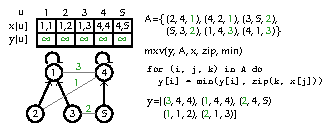
\includegraphics[width=0.9\textwidth]{figures/spmv-msf.pdf}
\caption{Illustration of the matrix-vector multiplication for min-edge picking. In \boruvka{}'s algorithm, matrix $\mathbf{A}$ is an undirected weighted graph and vector $x$ encodes both the supervertex id and the vertex's own id. The \emph{mxv} finds for each vertex $u$ the minimum tuple $(w, f[v], v)$ among the $v$'s in $u$'s adjacency list.}
\label{fig:spmv}
\end{figure}

\begin{figure}
\centering
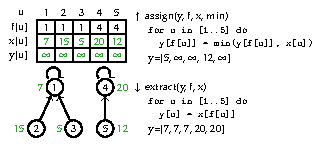
\includegraphics[width=0.9\textwidth]{figures/assign.pdf}
\caption{Illustration of the \emph{assign} and \emph{extract} operations (without a mask). In \boruvka{}'s algorithm, vector $f$ stores the supervertex of every vertex, which defines a flattened tree structure for each connected component. The \emph{assign} operation let every supervertex collect the minimum value in the whole tree, and the \emph{extract} operation let every vertex see the value on the root.}
\label{fig:assign}
\end{figure}

The linear algebra approach is yet another programming model for large-scale graph processing and has gained big success in some graph problems like the breadth-first search~\cite{graph500}.
However, this approach is currently less popular than the vertex-centric paradigm, which is probably due to the more abstract way of thinking required in the linear algebraic programming of graph algorithms.
This work tries to convince the readers that the linear algebra approach is actually very promising which can not only represent complex graph algorithms in an elegant way but also implement some graph computation more efficiently than the vertex-centric paradigm.

In this chapter, we propose two linear algebra algorithms, the FastSV algorithm for finding connected components in undirected graphs, and a linear algebra implementation of \boruvka{}'s algorithm for finding the minimum spanning forests in undirected weighted graphs.
Both algorithms are classic graph algorithms that have numerous applications in modern areas like biological data analysis~\cite{xu2002clustering,van2000graph}, cancer detection~\cite{kayser1993minimum,brinkhuis1997minimum}, computer vision~\cite{yang1989improved}, clustering algorithms~\cite{wang2009divide,zhong2010graph}, and scientific computing.
Our work not only enriches the set of problems the linear algebra approach can handle, but also provides the most scalable connected component algorithm and the most efficient minimum spanning tree forest in the literature of distributed graph computing, showing a promising future of the linear algebra approach in graph processing.


\section{The FastSV algorithm}
\label{sec:algo-two}

In this section, we introduce four important optimizations for the simplified SV algorithm, obtaining FastSV with faster convergence.

\subsection{A simplified SV algorithm }
\label{sec:algo-one}
\autoref{algo:algo-one} describes the simplified SV algorithm, which is the basis of our parallel algorithm. 
Initially, the parent $f[u]$ of a vertex $u$ is set to itself to denote $n$ single-vertex trees. 
We additionally maintain a copy $f_{\mathit{next}}$  of the parent vector so that the parallel algorithm reads from $f$ and writes to $f_{\mathit{next}}$.
Given a fixed ordering of vertices, each execution of \autoref{algo:algo-one} generates exactly the same pointer graph after the $i$th iteration because of using separate vectors for reading and writing. 
Hence, the convergence pattern of this parallel algorithm is completely deterministic, making it suitable for massively-parallel distributed systems.  
By contrast, concurrent reading from and writing to a single vector $f$ still deliver the correct connected components, but the structures of intermediate pointer graphs are not deterministic. 


%We give a high-level description of the simplified SV algorithm in \autoref{algo:algo-one}.
%The SV algorithm proceeds in rounds.
%It starts with $|V|$ singleton trees and iterates until the pointer graph (or we can say the parent vector $f$) stabilizes.
In each iteration, the algorithm performs tree hooking and shortcutting operations in order:
\begin{itemize}
\item \textbf{Tree hooking (line 6--8):} for every edge $(u,v)$, if $u$'s parent $f[u]$ is a root and $f[v]<f[u]$, then make $f[u]$ point to $f[v]$. As mentioned before, the updated parents are stored in a separate vector $f_{\mathit{next}}$ so the updated parents are not used in the current iteration. 
\item \textbf{Shortcutting (line 11--13):} if a vertex $u$ does not point to a root vertex, make $u$ point to its grandparent $f[f[u]]$.
\end{itemize}

The algorithm terminates when the parent vector remains unchanged in the latest iteration.
At termination, every tree becomes a star, and vertices in a star constitute a connected component. 
The correctness of this algorithm is discussed in previous work~\cite{greiner1994comparison}.
However, as mentioned before, without the unconditional hooking used in the original SV algorithm, we can no longer guarantee that \autoref{algo:algo-one} converges in $O(\log n)$ iterations. 
We will show in \autoref{sec:msf-eval} that \autoref{algo:algo-one} indeed converges slowly, but does not require the worst case bound $O(n)$ iterations for the practical graphs we considered. 
Nevertheless, the extra iterations needed by \autoref{algo:algo-one} increase the runtime of parallel SV algorithms. 
To alleviate this problem, we develop several novel hooking schemes, ensuring that the improved algorithm FastSV  is as simple as \autoref{algo:algo-one}, but the former converges faster than the latter.

\subsection{Optimizations to improve convergence}

\subsubsection{Hooking to grandparent}

\begin{figure}[t]
\centering
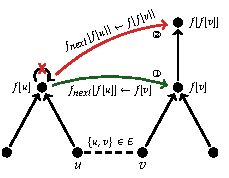
\includegraphics[width=0.5\textwidth]{figures/hooking.pdf}
\vspace{-10pt}
\caption{Two different ways of performing the tree hooking. (1) the original algorithm that hooks $u$'s parent $f[u]$ to $v$'s parent $f[v]$, (2) hook $u$'s parent $f[u]$ to $v$'s grandparent $f[f[v]]$. Both strategies are correct and the latter one improves the convergence.}
\vspace{-10pt}
\label{fig:hooking}
\end{figure}

In the original algorithm, the tree hooking is represented by the assignment $f_{\mathit{next}}[f[u]]\leftarrow f[v]$ (line 8 in \autoref{algo:algo-one}) requiring $f[u]$ to be a root vertex, $(u,v)\in E$ and $f[v]<f[u]$.
It is not hard to see, if we perform the tree hooking using $v$'s grandparent $f[f[v]]$, saying $f_{\mathit{next}}[f[u]]\leftarrow f[f[v]]$, the algorithm will still produce the correct answer.
To show this, we visualize both operations in \autoref{fig:hooking}.

Suppose $(u,v)$ is an edge in the input graph and $f[v]<f[u]$.
The original hooking operation is represented by the green arrow in the figure, which hooks $f[u]$ to $v$'s parent $f[v]$.
Then, our new strategy simply changes $f[v]$ to $v$'s grandparent $f[f[v]]$, resulting the red arrow from $f[u]$ to $f[f[v]]$.
It is not hard to see, as long as we choose a value like $f[f[v]]$ such that it is in the same tree of $v$, we can easily prove the correctness of the algorithm.
One can also expect that any value like $f^{k}[v]$ ($v$'s $k$-th level ancestor) will also work.

%The remaining question is that why we are interested in the hooking options other than $f[v]$, for example the $f[f[v]]$.
Intuitively, choosing a higher ancestor of $v$ in the tree hooking will likely create shorter trees, leading to faster convergence (all trees are stars at termination).
%improve the convergence because it creates shorter trees, leading to stars
However, finding higher ancestors may incur additional computational cost.  
%it may also increase the computation time of each iteration to find such ancestor for every vertex $v$.
%Therefore, the tradeoff between the convergence and computation time per iteration is important.
Here, we choose grandparents $f[f[v]]$ because they are needed in the shortcutting operation anyway; hence, using grandparents does not incur additional cost in the hooking operation.
%, since the grandparent of each vertex is needed not only in the detection of root vertex, but also in the shortcutting operation.
%Our new hooking strategy basically reuses the computed grandparent value for each $v$, which does not introduce any additional computation cost.

\begin{figure}
\centering
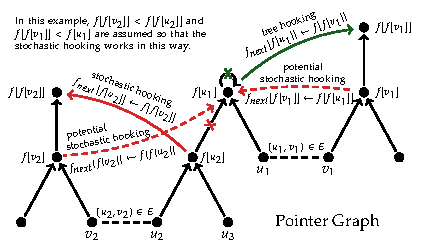
\includegraphics[width=0.75\textwidth]{figures/stochastic.pdf}
\caption{The stochastic hooking strategy.
Suppose there are two edges $(u_1,v_1)$ and $(u_2,v_2)$ activating the hooking operation.
The red arrows are the potential modifications to the pointer graph due to our stochastic hooking strategy, which tries to hook a non-root vertex to another vertex.
The solid line successfully modifies $f[u_2]$'s pointer to $f[f[v_2]]$, but the dashed lines do not take effect due to the ordering on the vertices.}
%The gray arrow is a standard hooking operation performed on root and the green arrow is introduced by our stochastic hooking strategy.
%This strategy also introduces two potential pointer modifications shown in red arrows, but due to the ordering on the vertices, they do not actually take place.}
\label{fig:stochastic}
\vspace{-10pt}
\end{figure}

\subsubsection{Stochastic hooking.}
The original SV algorithm and \autoref{algo:algo-one} always hooked the root of a tree onto another tree (see \autoref{fig:hooking} for an example).
Therefore, the hooking operation in \autoref{algo:algo-one} never breaks a tree into multiple parts and hooks different parts to different trees.
This restriction is enforced by the equality check $f[f[u]]=f[u]$ in line 7 of \autoref{algo:algo-one}, which is only satisfied by roots and their children. 
We observed that this restriction is not necessary for the correctness of the SV algorithm.
Intuitively, we can split a tree into multiple parts and hook them independently because these tree fragments will eventually be merged to a single connected component when the algorithm terminates. 
We call this strategy \emph{stochastic hooking}.



%Next, we are going to change the algorithm logic in a more aggressive way by removing the predicate $f[f[u]]=f[u]$ in the tree hooking.
%This is a rather aggressive strategy in the sense that it may disassemble the already computed connected components, but it also makes the algorithm converge faster in practice.

%The predicate $f[f[u]]=f[u]$ mainly has two effects in the original SV algorithm.
%First, it is used to decide which operation each vertex $u$ is to perform --- the tree hooking or the shortcutting.
%Then, the removal of the predicate basically means we perform both operations on every vertex. 
%Second, it also ensures that when performing the tree hooking, only the root vertices' pointers are changed, so that we always merge an entire connected component into another one.
%We no longer have such property when the predicate is removed, and therefore we name our new strategy as stochastic hooking.

The stochastic hooking strategy can be employed by simply removing the condition $f[f[u]]=f[u]$ from line 7 of \autoref{algo:algo-one}.
Then, any part of a tree is allowed to hook onto another vertex when the other hooking conditions are satisfied. 
It should be noted that after removing the condition $f[f[u]]=f[u]$, it is possible that a tree may hook onto a vertex in the same tree.
This will not affect the correctness though.
In this case, the effect of stochastic hooking is similar to the shortcutting, which hooks a vertex to some other vertex with a smaller identifier.

\autoref{fig:stochastic} shows an example of stochastic hooking by the solid red arrow from $f[u_2]$ to $f[f[v_2]]$.
In the original algorithm, $u_2$ does not modify its non-root parent $f[u_2]$'s pointer, but stochastic hooking changes $f[u_2]$'s pointer to one of $u$'s neighbor's grandparent $f[f[v_2]]$.
Suppose $f[u_1]$ points to $f[f[v_1]]$ after the tree hooking, we can see that $f[u_1]$ and $f[u_2]$ might be no longer in the same connected component (assuming $f[f[v_1]]$ and $f[f[v_2]]$ are in different trees).
Possible splitting of trees is a policy that differs from the conventional SV algorithm, but it gives a non-root vertex an opportunity to be hooked.
In \autoref{fig:stochastic}, $f[u_2]$'s new parent $f[f[v_2]]$ is smaller than $f[u_1]$, which can expedite the convergence.
%We do not consider this effect harmful.
%Instead, vertices are just finding the local minimals in a more independent way (not relying on the shortcutting operation only), and indeed $f[u_2]$'s new parent $f[f[v_2]]$ is smaller than $f[u_1]$, which is considered helpful to the convergence.
%we have more chances to proceed the algorithm.
%, which is a smaller grandparent vertex $f[f[v_2]]$ of $u$'s neighbors than $f[u_2]$'s current parent.
%The hooking result is represented by the green arrow from $f[u_2]$ to $f[f[v_2]]$.

\begin{comment}
Readers may notice that, if we insist on the original algorithm, vertex $f[u_2]$'s pointer will not be changed (since it is neither a root nor a vertex in the lower part), and in the next iteration it performs the shortcutting $f[f[u_2]]\leftarrow f[f[v_1]]$.
$u_2$ will not perform the tree merging as well, since it has to perform two shortcutting operations, first to its current grandparent $f[f[u_2]]$ then to $f[f[v_1]]$.
In this case, for the leftmost and rightmost trees, it is unlikely that one of them will hook to the other one quickly.
However, when performing the stochastic hooking, although $f[u_2]$ is detached from the original connected component rooted at $f[u_1]$, there is a high chance that in the next iteration $f[u_2]$ will change $f[f[v_2]]$'s pointer to $f[f[v_1]]$ (or vise versa depending on which one is larger) through an existing edge in the original connected component (from $f[u_2]$ to either $u_1$, $u_3$ or to $f[u_1]$), and then the vertices $f[f[v_1]]$ and $f[f[v_2]]$ will be in the same tree.
Therefore, even though the already recognized connected component may be disassembled due to the removal of the predicate, vertices can independently find local the local minimals and it may potentially help the convergence.
The values in the vector $f$ also decrease as the result of introducing more opportunities of hooking.
\end{comment}

\autoref{algo:algo-two} presents the high-level description of FastSV using the new hooking strategies.
Here, $\xleftarrow{\min}$ denotes a compare-and-assign operation that updates an entry of $f_{\mathit{next}}$ only when the right hand side is smaller.
The stochastic hooking is shown in line 6--7, and the shortcutting operation in line 12--13 is also affected by the removal of the predicate $f[f[u]]=f[u]$.



\begin{figure}
\centering
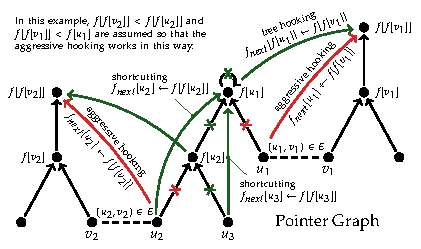
\includegraphics[width=0.75\textwidth]{figures/aggressive.pdf}
\caption{The aggressive hooking strategy.
Suppose there are two edges $(u_1,v_1)$ and $(u_2,v_2)$ activating the hooking operation.
The green arrows represent the hooking strategies introduced so far, and the red arrows represent our aggressive hooking strategy where a vertex may point at one of its neighbor's grandparent.
Some vertices may have multiple arrows (like $u_2$), and which vertex to hook onto is decided by the ordering on the vertices.}
%The new strategy may override the shortcutting operation (red arrow) or even the stochastic hooking operation, so in practice we decide which arrow to use by the ordering on vertices, where the smallest one is eventually used.}
\label{fig:aggressive}
\vspace{-10pt}
\end{figure}

\subsubsection{Aggressive hooking.}
Next, we give a vertex $u$ another chance to hook itself onto another tree whenever possible.
This strategy is called \emph{aggressive hooking}, performed by $f_{\mathit{next}}[u]\xleftarrow{\min} f[f[v]]$ for all $(u,v)\in E$.
\autoref{fig:aggressive} gives an example of aggressive hooking by the red arrow for $u_1$ and $u_2$.
Here, $u_1$'s pointer will not be modified by any hooking operation introduced so far.
Then, the aggressive hooking makes $u_1$ point to its newest grandparents $f[f[v_1]]$, as if an additional shortcutting is performed.
We should mention that the cost of an additional shortcutting $f'_{\mathit{next}}\leftarrow f_{\mathit{next}}[f_{\mathit{next}}]$ is expensive due to the recalculation of grandparents, while the aggressive hooking is essentially a cheap element-wise operation over $f$ by reusing some results in the stochastic hooking.
We will discuss how they are implemented \autoref{sec:sv-graphblas}.
%Note that an additional shortcutting operation $f\leftarrow f[f]$ is expensive due to the recalculation of grandparents, while the aggressive hooking $f\leftarrow \text{min}(f, \mathit{mngf})$ is just an element-wise multiplication of two vectors, which is easy to parallelize and highly scalable.
%, which is definitely preferable in our algorithm

For $u_2$ in \autoref{fig:aggressive}, it only performs the shortcutting operation $f_{\mathit{next}}[u_2]\leftarrow f[f[u_2]]$ in the original algorithm, and now the aggressive hooking performs $f_{\mathit{next}}[u_2]\leftarrow f[f[v_2]]$.
Our implementation let $f[u_2]$ point to the smaller one between $f[f[u_2]]$ and $f[f[v_2]]$, which is expected to give the best convergence for vector $f$.

\begin{algorithm}[t]
\small
\caption{The FastSV algorithm. \textbf{Input:} $G(V,E)$. \textbf{Output:} The parent vector $f$}
\label{algo:algo-two}
\begin{algorithmic}[1]
\Procedure {FastSV}{$V,E$}
\For {every vertex $u \in V$}
  \State $f[u], f_{\mathit{next}}[u] \leftarrow u$
\EndFor
\Repeat
  \State\Comment {Step 1: Stochastic hooking}
  \For {every $(u,v) \in E$} \textbf{in parallel}
    \State $f_\mathit{next}[f[u]] \xleftarrow{\min} f[f[v]]$
  \EndFor
  \State\Comment {Step 2: Aggressive hooking}
  \For {every $(u,v) \in E$} \textbf{in parallel}
    \State $f_{\mathit{next}}[u] \xleftarrow{\min} f[f[v]]$
  \EndFor
  \State\Comment {Step 3: Shortcutting}
  \For {every $u \in V$} \textbf{in parallel}
    \State $f_{\mathit{next}}[u] \xleftarrow{\min} f[f[u]]$
  \EndFor
  \State $f\leftarrow f_{\mathit{next}}$
\Until{$f[f]$ remains unchanged}
\EndProcedure
\end{algorithmic}
\end{algorithm}

\subsubsection{Early termination.}
\label{sec:termination}

The last optimization is a generic one that applies to most variations of the SV algorithm.
SV's termination is based on the stabilization of the parent vector $f$, which means even if $f$ reaches the converged state (where every vertex points to the smallest vertex in its connected component), we need an additional iteration to verify that.
We will see in \autoref{sec:convergence} that for most real-world graphs, FastSV usually takes 5 to 10 iterations to converge.
Hence, this additional iteration can consume a significant portion of the runtime. % really matters.
The removal of the last iteration is possible by detecting the stabilization of the grandparent $f[f]$ instead of $f$.
The following lemma ensures the correctness of this new termination condition.
\begin{lemma}\label{thm1}
After an iteration, if the grandparent $f[f]$ remains unchanged, then the vector $f$ will not be changed afterwards.
\end{lemma}

The proof makes use of the following lemmas.

\begin{lemma}\label{lemma1}
During the whole algorithm, $f[u]\leq u$ holds for all vertices $u$.
\end{lemma}

\begin{proof}
Initially, $f[u]=u$ for all vertex $u$ and the lemma holds trivially.
The the operation $\xleftarrow{\min}$ ensures that $f$ can only decrease, so the lemma always holds.
\end{proof}

\begin{comment}
\begin{lemma}\label{lemma2}
After an iteration, if the grandparent $f[f]$ remains unchanged, then no vertex directly pointing to a root (including the root itself) has changed its pointer.
\end{lemma}

\begin{proof}
By contradiction.
Suppose a vertex $u$ changes its pointer to some $v$, then the operation $\xleftarrow{\min}$ ensures that $v<f[u]$.
Since $u$ points to a root $f[u]$ in the previous iteration, then $u$'s previous grandparent $f[f[u]]$ equals to $f[u]$.
However, $f_{\mathit{next}}[v] \leq v < f[f[u]]$ by \cref{lemma1}, so $u$'s new grandparent $f_{\mathit{next}}[v]$ is different from $f[f[u]]$.
\end{proof}
\end{comment}

\begin{lemma}\label{lemma3}
After an iteration, if the grandparent $f[f]$ remains unchanged, then every vertex hooks onto its grandparent in the previous operation.
\end{lemma}

\begin{proof}
By contradiction.
Suppose $u$ changes its pointer to some $v$ other than $f[f[u]]$, then since it overrides the shortcutting operation $f_{\mathit{next}}[u]\xleftarrow{\min}f[f[u]]$ we know that $v<f[f[u]]$.
By \cref{lemma1}, $u$'s new grandparent $f_{\mathit{next}}[v]\leq v<f[f[u]]$, then the grandparent of $u$ is changed.
\end{proof}

\begin{lemma}\label{lemma4}
After an iteration, if the grandparent $f[f]$ remains unchanged, then every vertex points to a root now.
\end{lemma}

\begin{proof}
By contradiction.
Suppose $u$'s new parent $v$ is not a root, then $u$'s new grandparent is $f_{\mathit{next}}[v]<v=f[f[u]]$ (by \cref{lemma1} and \cref{lemma3}), which means $u$'s grandparent has changed.
\end{proof}

Here we prove \cref{thm1}.

\begin{proof}
We show that no hooking operation will be performed if $f[f]$ remains unchanged after an iteration.
The aggressive hooking in the form of $f_{\mathit{next}}[u]\xleftarrow{\min}f[f[v]]$ is overridden by the shortcutting operation $f_{\mathit{next}}[u]\xleftarrow{\min}f[f[u]]$ in the previous iteration (by \cref{lemma3}), meaning that $f[f[u]]\leq f[f[v]]$ for all $(u,v)\in E$.
Since then, $f[f]$ is not changed, so the aggressive hooking will not be performed in the current iteration either.
The stochastic hooking $f_{\mathit{next}}[f[u]]\xleftarrow{\min}f[f[v]]$ will not be performed since for all $(u,v)\in E$ we have $f[f[u]]\leq f[f[v]]$.
Shortcutting will not be performed either since every vertex points to a root now (by \cref{lemma4}).
Then, no hooking operation can be performed, and the vector $f$ remains unchanged afterwards.
\end{proof}

In practice, we found that on most practical graphs, FastSV identifies all the connected components before converged, and the last iteration always performs the shortcutting operation to turn the trees into stars.
In such case, the grandparent vector $f[f]$ converges one iteration earlier than $f$.


\subsection{A linear algebra formulation}
\label{sec:sv-graphblas}

%We first give an informal description of GraphBLAS's APIs used in our algorithm.
%Formal descriptions can be found in the API document~\cite{graphblas}.
In GraphBLAS, we assume that the vertices are indexed from $0$ to $|V|-1$, then the vertices and their associated values are stored as GraphBLAS object \texttt{GrB\_Vector}.
The graph's adjacency matrix is stored as a GraphBLAS object \texttt{GrB\_Matrix}.
For completeness, we concisely describe the GraphBLAS functions used in our implementation below, where the formal descriptions of these functions can be found in the API document~\cite{graphblas}.
We use $\emptyset$ to denote \texttt{GrB\_NULL}, which is fed to those ignored input parameters.
\begin{itemize}
\item
  The function $\texttt{GrB\_mxv}(\mathit{y}, \emptyset, \text{accum}, \text{semiring}, \mathbf{A}, \mathit{x}, \emptyset)$ multiplies the matrix $\mathbf{A}$ with the vector $\mathit{x}$ on a semiring and outputs the result to the vector $\mathit{y}$.
  When the accumulator (a binary operation \textit{accum}) is specified, the multiplication result is combined with $y$'s original value instead of overwriting it.
\item
  The function $\texttt{GrB\_extract}(\mathit{y}, \emptyset, \emptyset, \mathit{x}, \text{index}, \text{n}, \emptyset)$ extracts a sub-vector $y$ from the specified positions in an input vector $x$.
  We can regard this operation as $y[i]\leftarrow x[\text{index}[i]]$ for $i\in[0\isep n-1]$ where $n$ is the length of the array $\mathit{index}$ and also the vector $\mathit{y}$.
\item
  The function $\texttt{GrB\_assign}(\mathit{y}, \emptyset, \text{accum}, \mathit{x}, \text{index}, \text{n}, \emptyset)$ assigns the entries from the input vector $x$ to the specified positions of an output vector $y$.
  We can regard it as $y[\text{index}[i]]\leftarrow x[i]$ for $i\in[0\isep n-1]$ where $n$ is the length of the array $\mathit{index}$ and also the vector $x$.
  $\mathit{accum}$ is the same as the one in \texttt{GrB\_mxv}.
\item
  The function $\texttt{GrB\_eWiseMult}(\mathit{y}, \emptyset, \emptyset, \text{binop}, \mathit{x}_1, \mathit{x}_2, \emptyset))$ performs the element-wise (generalized) multiplication on the intersection of elements of two vectors $x_1$ and $x_2$ and outputs the vector $y$.
\item
  The function $\texttt{GrB\_Vector\_extractTuples}(\text{index}, \text{value},$ $\&\text{n}, f)$ extracts the nonzero elements (tuples of index and value) from vector $f$ into two separate arrays $\mathit{index}$ and $\mathit{value}$.
  It returns the element count to $n$.
\end{itemize}
For the rest functions, we have \texttt{GrB\_Vector\_dup} to duplicate a vector, \texttt{GrB\_reduce} to reduce a vector to a scalar value through a user-specified binary operation, and \texttt{GrB\_Matrix\_nrows} to obtain the dimension of a matrix.


\begin{comment}
\begin{itemize}
\item
  The function \texttt{GrB\_mxv} multiplies a matrix $\mathbf{A}$ with a vector $\mathit{x}$ on a semiring, producing a vector $\mathit{y}$.
  The parameters are $(\mathit{y}, \emptyset, \text{accum}, \text{semiring}, \mathbf{A}, \mathit{x}, \emptyset)$, containing the output vector $y$, an optional accumulator (when specified, the output vector's original value is also used in the computation), a user-specified semiring, and the input matrix $\mathbf{A}$ and vector $\mathit{x}$.
  Here, $\emptyset$ denotes \texttt{GrB\_NULL} and is fed to those ignored input parameters.
  A semiring is a  \texttt{GrB\_Semiring} object defined by a pair of operations $(\text{multiply}, \text{add})$.
  In our algorithm, we always use the (select2nd, min) semiring, whose graph semantics is to capture for each vertex (in the output vector) the minimum value of all its neighbors from the input vector.
\item
  The function \texttt{GrB\_extract} has the parameters $(\mathit{y}, \emptyset, \emptyset, \mathit{x}, \text{index}, \text{n}, \emptyset)$, which extracts a sub-vector $y$ from the specified positions in an input vector $x$.
  We can regard this operation as $y[i]\leftarrow x[\text{index}[i]]$.
  The array $\mathit{index}$ contains the indices we want to extract and $n$ is the length of $\mathit{index}$ and also the vector $\mathit{y}$.
\item
  The function \texttt{GrB\_assign} has the parameters $(\mathit{y}, \emptyset, \mathit{accum}, \mathit{x}, \text{index}, \text{n}, \emptyset)$ , which assigns the entries from the input vector $x$ to the specified positions of an output vector $y$, namely $y[\text{index}[i]]\leftarrow x[i]$.
  $n$ is the length of the array $\mathit{index}$ and also the vector $x$, and the optional accumulator $\mathit{accum}$ is the same as the one in \texttt{GrB\_mxv}, which performs $y[i]\leftarrow \mathit{accum}(y[i], v)$ instead of assignment when specified.
\item
  The function \texttt{GrB\_eWiseMult} has the parameters $(\mathit{y}, \emptyset, \mathit{accum}, \mathit{binop}, \mathit{x}_1, \mathit{x}_2, \emptyset))$, which performs the element-wise (generalized) multiplication on the intersection of elements of two vectors $x_1$ and $x_2$, and the result vector $y$ is calculated by $y[i]\leftarrow \mathit{binop}(x_1[i], x_2[i])$.
  Here $\mathit{binop}$ is a user-specified binary operation and $\mathit{accum}$ is an optional accumulator.
\end{itemize}
\end{comment}

\autoref{algo:graphblas2} describes the  FastSV algorithm in GraphBLAS.
Before every iteration, we calculate the initial grandparent $\mathit{gf}$ for every vertex.
\begin{comment}
First, in line 7--8, we compute the grandparent $\mathit{gf}[u]\leftarrow f[f[u]]$ for every vertex $u$, which is needed for the stochastic hooking and the shortcutting operations.
It is implemented by the \texttt{GrB\_extract} function in line 8 where the indices $f[v]$ are the values of $f$ extracted in line 7.
The result is stored in the vector $\mathit{gf}$.
\end{comment}
First, we perform the stochastic hooking in line 10--11.
GraphBLAS has no primitive that directly implements the parallel-for on an edge list (line 9 in \autoref{algo:algo-two}), so we have to first aggregate $v$'s grandparent $\mathit{gf}[v]$ to vertex $u$ for every $(u,v)\in E$, obtaining the vector $\mathit{mngf}[u]=\min_{v\in N(u)}\mathit{gf}[v]$.
This can be implemented by a matrix-vector multiplication $\mathit{mngf}=\textbf{A}\cdot\mathit{gf}$ using the (select2nd, min) semiring.
Next, the hooking operation is implemented by the assignment $f[f[u]]\leftarrow \mathit{mngf}[u]$ for every vertex $u$.
This is exactly the \texttt{GrB\_assign} function in line 10 where the indices are the values of vector $f$ extracted in either line 5 before the first iteration or line 16 from the previous iteration.
The accumulator \texttt{GrB\_MIN} prevents the nondeterminism caused by the modification to the same entry of $f$, and the minimum operation gives the best convergence in practice.

Aggressive hooking is then implemented by an element-wise multiplication $f\leftarrow \min(f,\mathit{mngf})$ in line 13.
Although it is another operation in FastSV that performs the parallel-for on an edge list, it can reuse the vector $\mathit{mngf}$ computed in the previous step, so the aggressive hooking is actually efficient.
Shortcutting is also implemented by an the element-wise multiplication $f\leftarrow \text{min}(f,\mathit{gf})$ in line 15.
Next, we calculate the grandparent vector $\mathit{gf}[u]\leftarrow{f[f[u]]}$.
It is implemented by the \texttt{GrB\_extract} function in line 18 where the indices are the values of $f$ extracted in line 17.

%An alternative is to perform an assignment $f\leftarrow \mathit{gf}$ on those vertices $v$ , but the two implementations are equivalent.
%The reason is that, although the \texttt{GrB\_eWiseMult} may additionally affect the vertices that are pointing to a root, these nodes already have $f=\mathit{gf}$ at the beginning of the iteration, and the root vertices' $f$ can only decrease in the previous two steps, so the \texttt{GrB\_eWiseMult} actually has no effect on them.

At the end of each iteration, we calculate the number of modified entries in $\mathit{gf}$ in line 20 -- 21 to check whether the algorithm has converged or not.
A copy of $\mathit{gf}$ is stored in the vector $\mathit{dup}$ for determining the termination in the next iteration.

\begin{algorithm}[t]
\small
\caption{The linear algebra FastSV algorithm. \textbf{Input:} The adjacency matrix $\mathbf{A}$ and the parent vector $f$. \textbf{Output:} The parent vector $f$.}
\label{algo:graphblas2}
\begin{algorithmic}[1]
\Procedure {FastSV}{$\mathbf{A},f$}
\State \text{GrB\_Matrix\_nrows} $(\&\text{n}, \mathbf{A})$
\State \text{GrB\_Vector\_dup} $(\&\mathit{gf}, \mathit{f})$ \Comment {initial grandparent}
\State \text{GrB\_Vector\_dup} $(\&\mathit{dup}, \mathit{gf})$ \Comment {duplication of $\mathit{gf}$}
\State \text{GrB\_Vector\_dup} $(\&\mathit{mngf}, \mathit{gf})$
\State \text{GrB\_Vector\_extractTuples} $(\text{index}, \text{value}, \&\text{n}, f)$
\State {$\text{Sel2ndMin}\leftarrow \text{a (select2nd, Min) semiring}$}
\Repeat
  \State \Comment {Step 1: Stochastic hooking}
  \State \text{GrB\_mxv} $(\mathit{mngf}, \emptyset, \text{GrB\_MIN}, \text{Sel2ndMin}, \mathbf{A}, \mathit{gf}, \emptyset)$
  \State \text{GrB\_assign} $(f, \emptyset, \text{GrB\_MIN}, \mathit{mngf}, \text{value}, \text{n}, \emptyset)$
  \State \Comment {Step 2: Aggressive hooking}
  \State \text{GrB\_eWiseMult} $(f, \emptyset, \emptyset, \text{GrB\_MIN}, f, \mathit{mngf}, \emptyset)$
  \State \Comment {Step 3: Shortcutting}
  \State \text{GrB\_eWiseMult} $(f, \emptyset, \emptyset, \text{GrB\_MIN}, f, \mathit{gf}, \emptyset)$
  \State \Comment {Step 4: Calculate grandparents}
  \State \text{GrB\_Vector\_extractTuples} $(\text{index}, \text{value}, \&\text{n}, f)$
  \State \text{GrB\_extract} $(\mathit{gf}, \emptyset, \emptyset, f, \text{value}, \text{n}, \emptyset)$
  \State \Comment {Step 5: Check termination}
  \State \text{GrB\_eWiseMult} $(\mathit{diff}, \emptyset, \emptyset, \text{GxB\_ISNE}, \mathit{dup}, \mathit{gf}, \emptyset)$
  \State \text{GrB\_reduce} $(\&\text{sum}, \emptyset, \text{Add}, \mathit{diff}, \emptyset)$
    \State \text{GrB\_assign} $(\text{dup}, \emptyset, \emptyset, \mathit{gp}, \text{GrB\_ALL}, 0, \emptyset))$
\Until {$\text{sum}=0$}
\EndProcedure
\end{algorithmic}
\end{algorithm}

\subsection{A distributed implementation using CombBLAS}
\label{sec:sv-combblas}

The distributed version of FastSV is implemented in CombBLAS~\cite{combblas}.
CombBLAS provides all operations needed for FastSV, but its API differs from the GraphBLAS standard.
GraphBLAS's \textit{collections} (matrices and vectors) are opaque datatypes whose internal representations (sparse or dense) are not exposed to users, but CombBLAS distinguishes them in the user interface.
Then, GraphBLAS's functions often consist of multiple operations (like masking, accumulation and the main operation) as described in \autoref{sec:sv-graphblas}, while in CombBLAS we usually perform a single operation at a time.
Despite these differences, a straightforward implementation of FastSV on CombBLAS can be obtained by transforming each GraphBLAS function to the semantically equivalent ones in CombBLAS, using dense vectors in all scenarios.

The parallel complexity of the main linear algebraic operations used in FastSV (the vector variants of \texttt{GrB\_extract} and \texttt{GrB\_assign}, and the \texttt{GrB\_mxv}), as well as the potential optimizations are discussed in the LACC paper~\cite{lacc}.
Due to the similarity of FastSV and LACC in the algorithm logic, they can be optimized by the similar optimization techniques.
We briefly summarize them below.

\textbf{Broadcasting-based implementation for the extract and assign operations.}
The \emph{extract} and \emph{assign} operations fetch or write data on the specified locations of a vector, which may cause a load balancing issue when there is too much access on a few locations.
In FastSV, these locations are exactly the set of parent vertices in the pointer graph, and due to the skewed structure of the pointer graph, the root vertices (especially those belonging to a large component) will have extremely high workload.
When using the default \emph{assign} and \emph{extract} implementations in CombBLAS via all-to-all communication, several processes become the bottleneck and slow down the whole operation significantly.
The solution is a manual implementation of these two operations via the detection of the hot spots and broadcasting the entries on those processes.

\textbf{Taking advantage of the sparsity.}
The matrix-vector multiplication $\mathit{mngf}=\mathbf{A}\cdot\mathit{gf}$ is an expensive operation in FastSV (see our performance profiling in \autoref{sec:sparsity}).
The straightforward implementation naturally chooses the sparse-matrix dense-vector (SpMV) multiplication, since all the vectors in FastSV are dense vectors.
Alternatively, we can use an incremental implementation by computing $\Delta\mathit{mngf}=\mathbf{A}\cdot(\Delta\mathit{gf})$, where $\Delta\mathit{gf} = \mathit{gf} - \mathit{gf}_{\mathit{prev}}$ containing only the modified entries of $\mathit{gf}$ is stored as a sparse vector, so the multiplication is the sparse-matrix sparse-vector multiplication (SpMSpV)~\cite{azad2017work}.
Depending on the sparsity of $\Delta\mathit{gf}$, SpMSpV could have much lower computation and communication cost than SpMV.
We use a threshold on the portion of modified entries of $\mathit{gf}$ to decide which method to use in each iteration, which effectively reduces the computation time.
\autoref{sec:sparsity} presents a detailed evaluation.

\begin{comment}
\begin{itemize}
\item the potential load balancing issue of the parallel \texttt{extract} and \texttt{assign} operation (fetching or writing data on specified locations of a vector) caused by too much access on a few locations, which is greatly amplified by FastSV's algorithm logic;
\item the high computational cost due to the lack of an important optimization that makes use of the sparsity, in particular using \textit{SpMSpV}.
\end{itemize}

Both optimizations are introduced in the LACC paper~\cite{lacc} and we implement them in our FastSV program.
Briefly speaking, for the load balancing issue, we detect the hot spots and broadcast the entries on those processes.
For the sparsity optimization, we implement the matrix-vector multiplication (line 10 in \autoref{algo:graphblas2}) in an incremental way using $\Delta\mathit{mngf}=\mathbf{A}\cdot\Delta\mathit{gf}$.
It is based on the observation that in late iterations $\Delta\mathit{gf} = \mathit{gf} - \mathit{gf}_{\mathit{prev}}$ is usually very sparse, then the sparsity of the input vector $\Delta\mathit{gf}$ accelerates the multiplication.

\todo{put my code in these two repository?}
Distributed-memory FastSV code that is used in our experiments is publicly available as part of the CombBLAS library\footnote{\url{https://bitbucket.org/berkeleylab/combinatorial-blas-2.0}}.
A simplified unoptimized serial GraphBLAS implementation is also committed to the LAGraph Library\footnote{\url{https://github.com/GraphBLAS/LAGraph}} for educational purposes.
\end{comment}

\begin{figure}
\centering
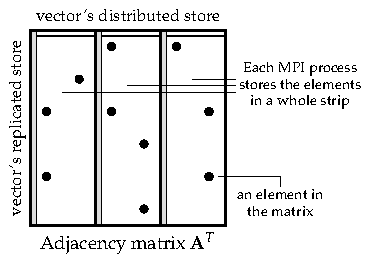
\includegraphics[width=0.5\textwidth]{figures/spmat.pdf}
\caption{Data placement of the matrix and vector.
The matrix is divided by column so that each MPI process stores the elements on a whole strip in the figure. For the vectors, they can be either replicated on all the processes, or split into disjoint segments and distributed on all the processes.}
\vspace{-8pt}
\label{fig:spmat}
\end{figure}

\begin{comment}
In this section, we present a distributed-memory implementation for \boruvka{}'s algorithm using MPI and OpenMP through the parallelization of the linear algebra operations.
For the complete MSF computation, we show an $O((m+np)\log(n))$ computation cost and $O(np)$ communication cost, both of which are much less than a Pregel implementation.
The computation cost here is measured by the total amount of vertices and edges visited by any process, and the communication cost is the total amount of messages sent out from any process.
Both numbers do not indicate the parallel execution time, but can give us a hint on the overall complexity of our implementation.
\end{comment}

%the data distribution method in those libraries are not suitable for \boruvka{}'s algorithm
%Furthermore, a straightforward operation-wise translation to the distributed-memory may actually suffer a huge performance penalty.
%We did not use an operation-wise translation but design a novel approach to implement \boruvka{}'s algorithm on distributed-memory and shows how the idea of fusion can optimize the implementation, and we show that \boruvka{}'s distributed-memory achieves an $O(m\log(n))$.

\section{Evaluation of FastSV}
\label{sec:fastsv-evaluation}

\begin{table}[t]
\centering
\caption{Graph datasets used to evaluate the parallel connected component algorithms.}
\vspace{-5pt}
\footnotesize
\label{tab:datasets}
\begin{tabular}{lrrrl}
\hline
Graph & Vertices & Edges & CCs & Description \\
\hline
%DBpedia & 18.27M & 136.54M & 1365 & The DBpedia hyperlink graph~\cite{konect} \\
Queen\_4147 & 4.15M & 166.82M & 1 & 3D structural problem~\cite{davis2011university} \\
kmer\_A2a & 170.73M & 180.29M & 5353 & Protein k-mer graphs from GenBank~\cite{davis2011university} \\
archaea & 1.64M & 204.78M & 59794 & archaea protein-similarity network~\cite{hipmcl} \\
kmer\_V1r & 214.01M & 232.71M & 9 & Protein k-mer graphs, from GenBank~\cite{davis2011university} \\
%mawi & 226.20M & 240.02M & 3971144 & \\
HV15R & 2.02M & 283.07M & 1 & Computational Fluid Dynamics Problem~\cite{davis2011university} \\
uk-2002 & 18.48M & 298.11M & 1990 & 2002 web crawl of .uk domain~\cite{davis2011university} \\
eukarya & 3.24M & 359.74M & 164156 & eukarya protein-similarity network~\cite{hipmcl} \\
uk-2005 & 39.45M & 936.36M & 7727 & 2005 web crawl of .uk domain~\cite{davis2011university} \\
twitter7 & 41.65M & 1.47B & 1 & twitter follower network~\cite{davis2011university} \\
SubDomain & 82.92M & 1.94B & 246969 & 1st-level subdomain graph extracted from Hyperlink~\cite{meusel2014graph} \\
sk-2005 & 50.64M & 1.95B & 45 & 2005 web crawl of .sk domain~\cite{davis2011university} \\
MOLIERE\_2016 & 30.22M & 3.34B & 4457 & automatic biomedical hypothesis generation system~\cite{davis2011university} \\
Metaclust50 & 282.20M & 37.28B & 15982994 & similarities of proteins in Metaclust50~\cite{hipmcl} \\
Hyperlink & 3.27B & 124.90B & 29360027 & hyperlink graph extract from the Common Crawl~\cite{meusel2014graph}\\
\hline
\end{tabular}
\end{table}

\begin{figure}[t]
\centering
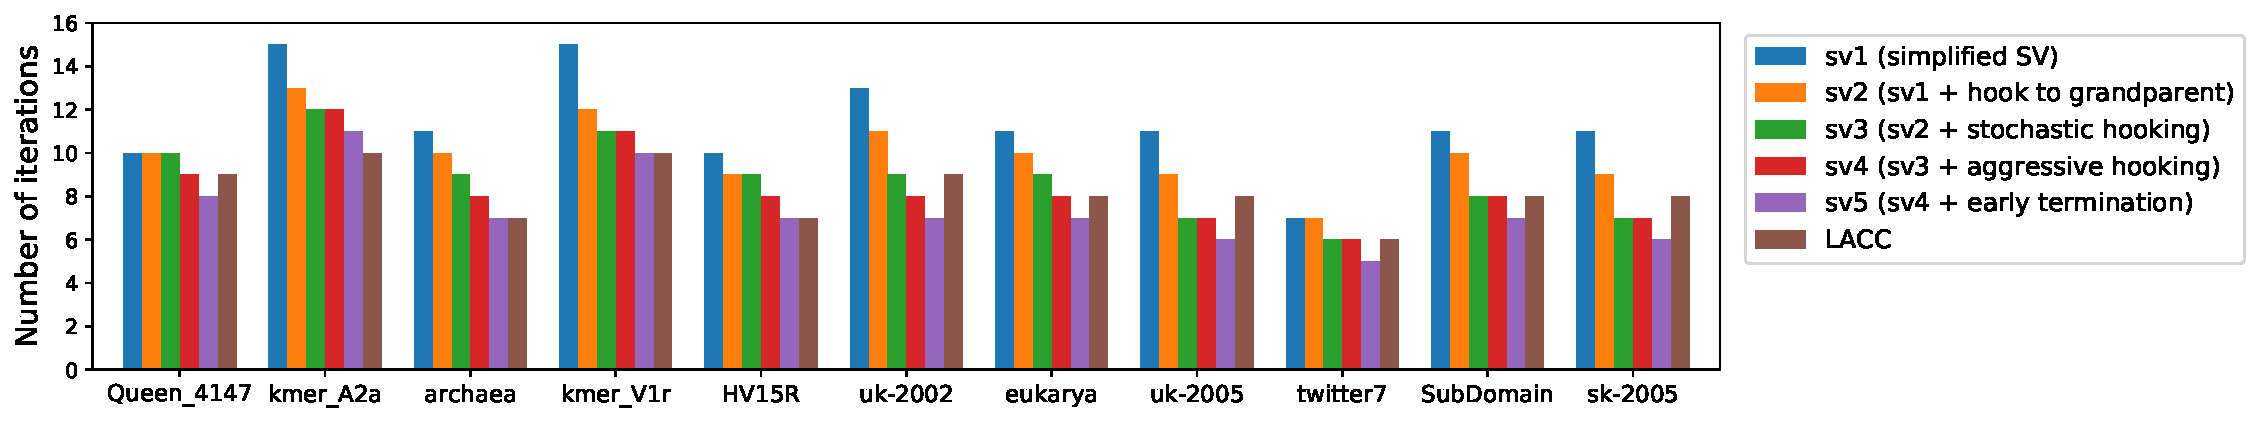
\includegraphics[width=1.0\textwidth]{figures/sv_iters.pdf}
\vspace{-20pt}
\caption{Number of iterations the simplified SV takes after performing each of the optimizations (sv5 is exactly our \Name{} algorithm), and the number of iterations LACC takes.}
\vspace{-10pt}
\label{fig:sv-iters}
\end{figure}

\begin{figure}[t]
\centering
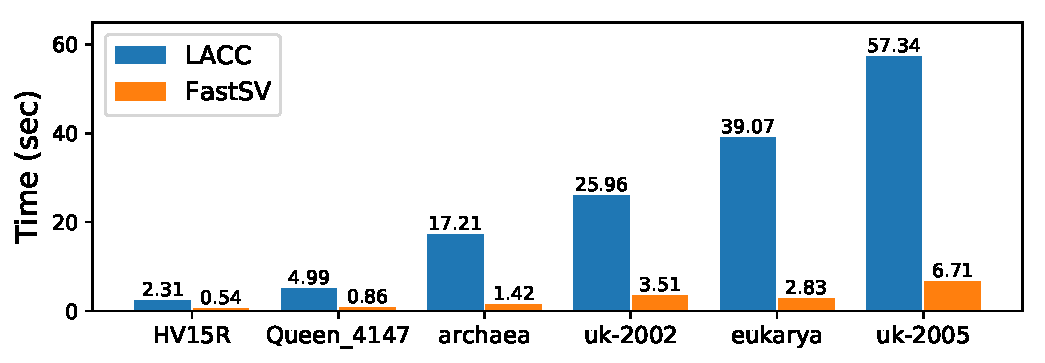
\includegraphics[width=0.8\textwidth]{figures/LAGraph.pdf}
\vspace{-5pt}
\caption{Performance of the parallel \Name{} and LACC in SuiteSparse:GraphBLAS on six small graphs.}
\vspace{-10pt}
\label{fig:LAGraph}
\end{figure}

\begin{figure}[t]
\centering
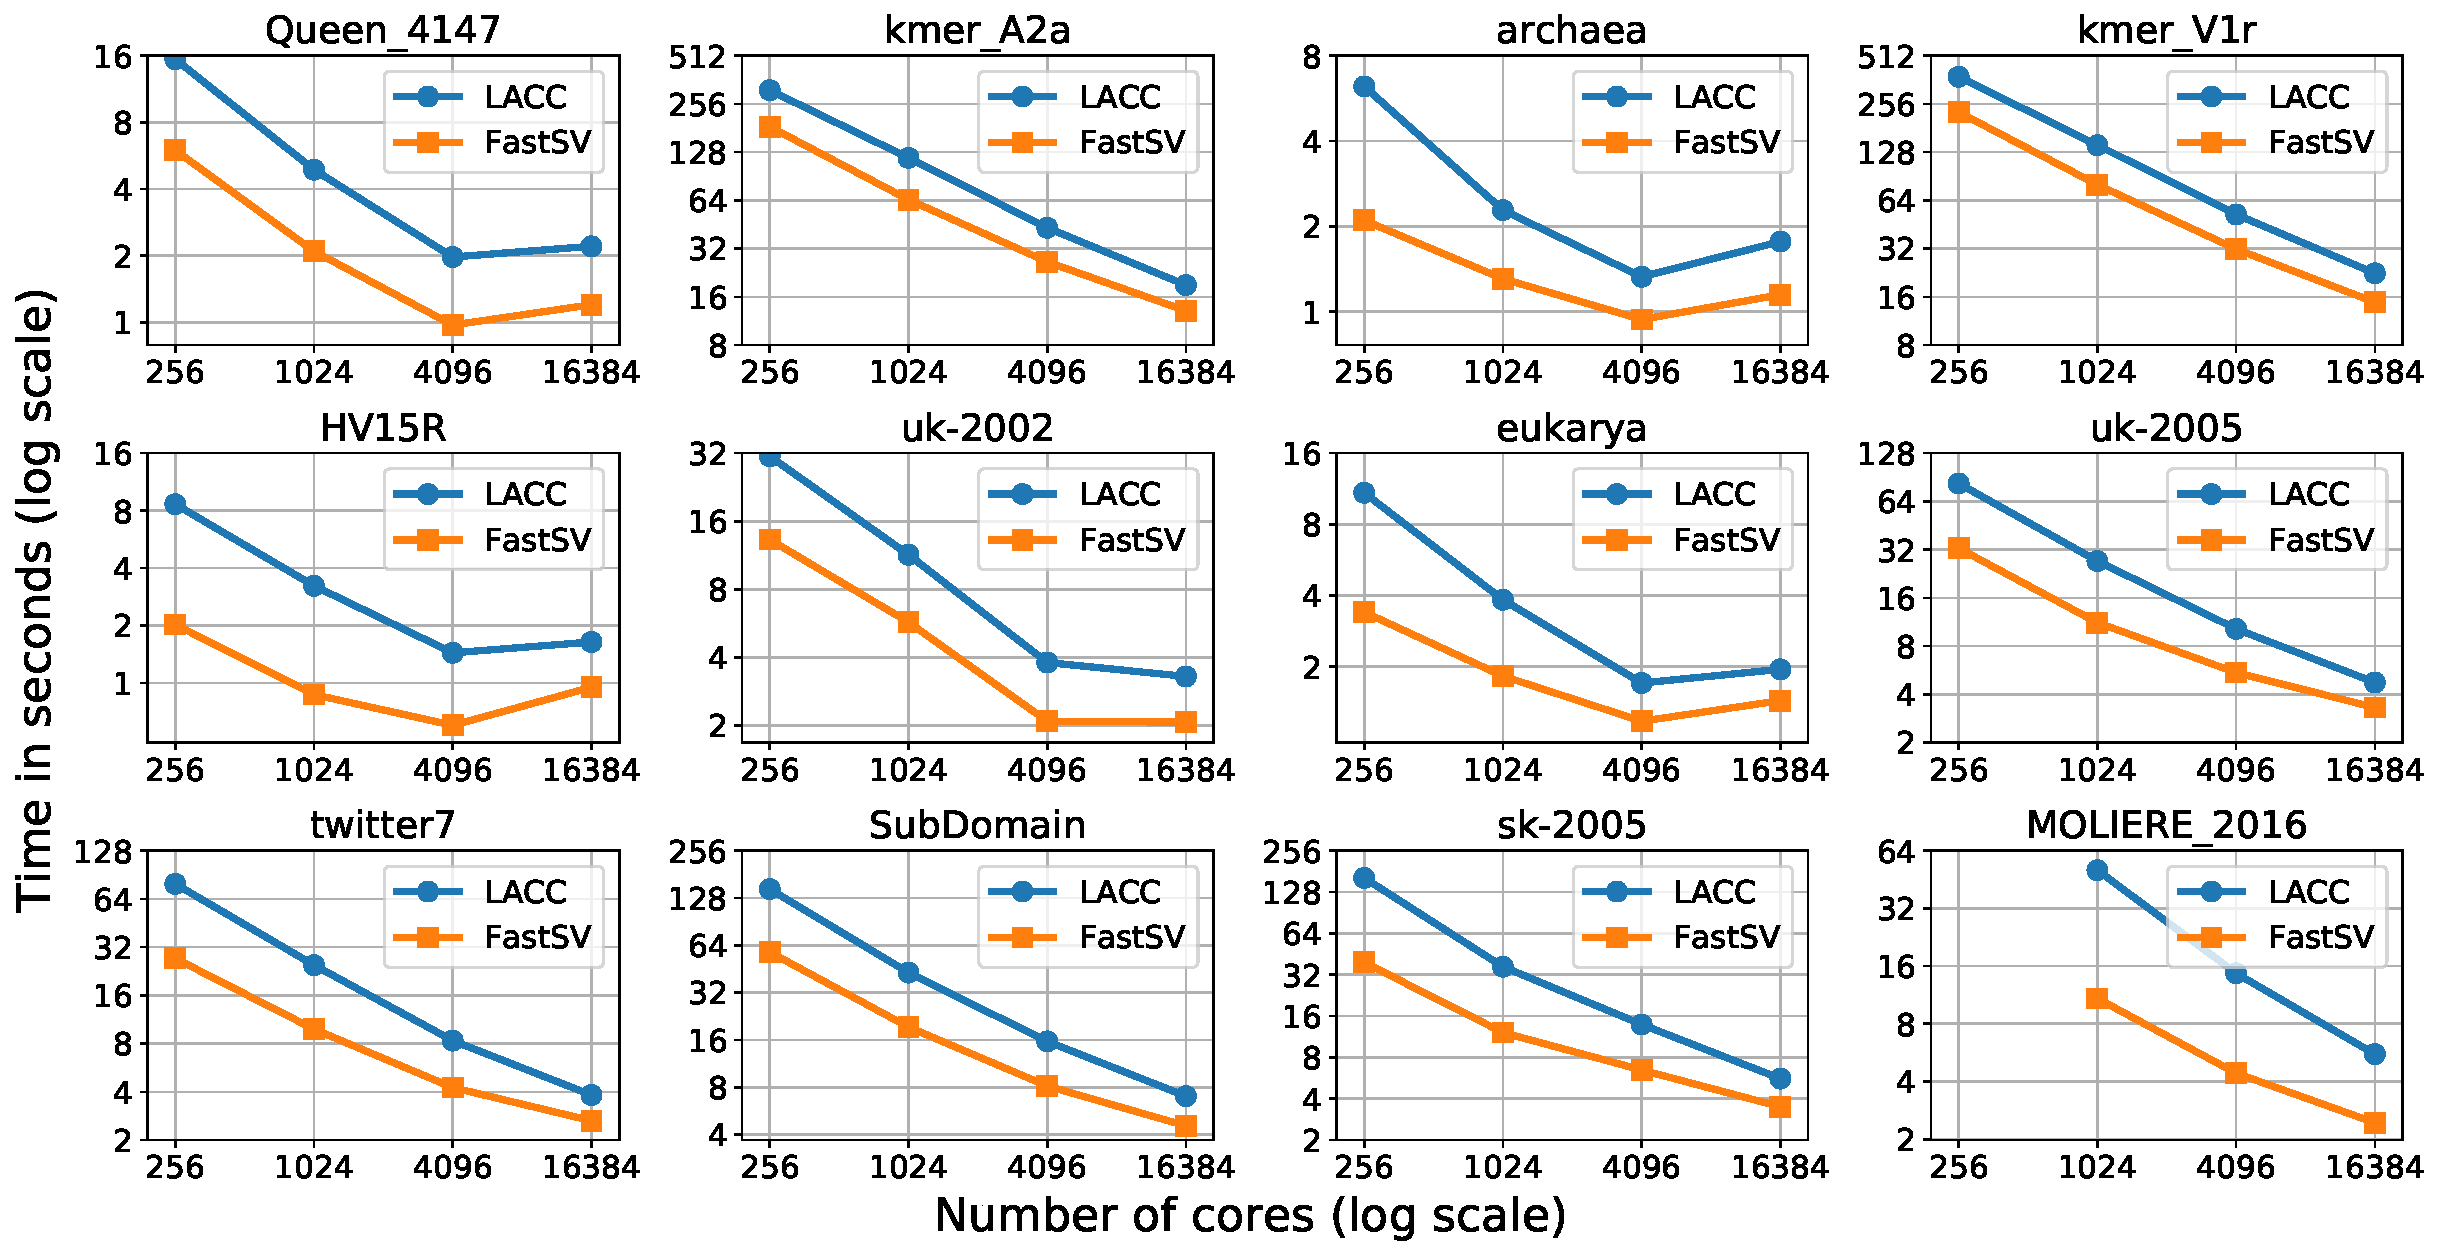
\includegraphics[width=\textwidth]{figures/scalability.pdf}
\vspace{-5pt}
\caption{Strong scaling of distributed-memory \Name{} and LACC using up to $16384$ cores (256 nodes).}
\vspace{-10pt}
\label{fig:scalability}
\end{figure}

\begin{figure}[t]
\centering
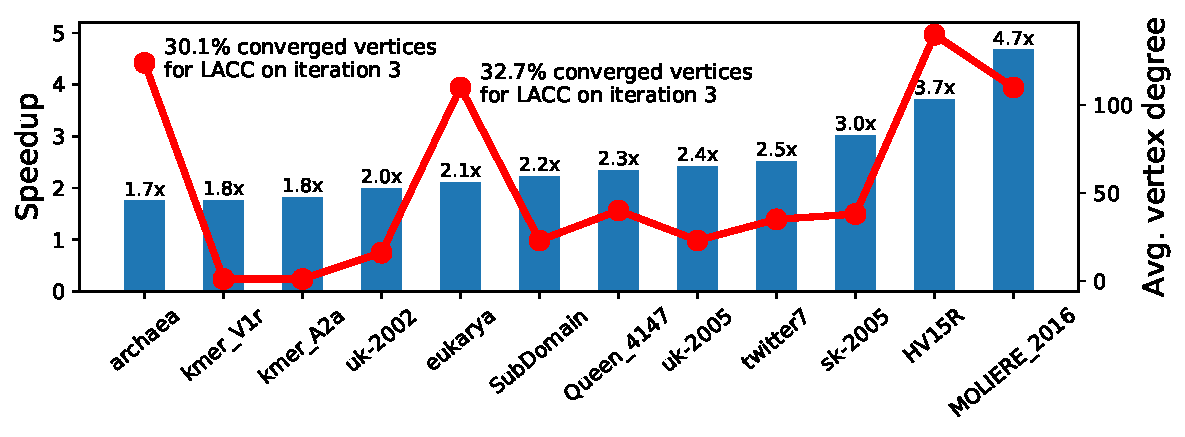
\includegraphics[width=0.8\textwidth]{figures/density-speedup.pdf}
\vspace{-5pt}
\caption{The speedup of \Name{} over LACC on twelve small datasets using 256 cores (bar chart) and each graph's density in terms of average vertex degree (line chart). A positive correlation between the two metrics can be observed, except for the two outliers \textit{archaea} and \textit{eukarya}.} %where LACC makes use of the detection of converged connected components to accelerate its execution.}
\vspace{-10pt}
\label{fig:density-speedup}
\end{figure}

\begin{comment}
\begin{figure}[t]
\centering
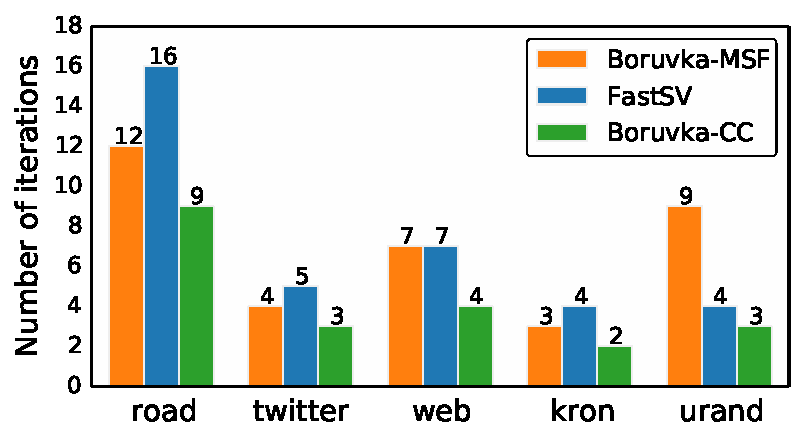
\includegraphics[width=0.48\textwidth]{figures/iterations.pdf}
\caption{Number of iterations \Name{} and LACC take on fourteen real-world graph datasets.}
\label{fig:iterations}
\end{figure}
\end{comment}

In this section, we evaluate various aspects of \Name{} showing its fast convergence, shared- and distributed-memory performance, scalability and several other performance characteristics.
We compare \Name{} with LACC~\cite{lacc} that has demonstrated superior performance over other distributed-memory parallel CC algorithms. 
%because the latter has already 
%The competitor we choose is LACC~\cite{lacc}, the state-of-the-art linear algebraic connected component algorithm prior to our work.
\autoref{tab:datasets} shows a diverse collection of large graphs used to evaluate CC algorithms. 
To the best of out knowledge, the Hyperlink graph~\cite{meusel2014graph} with 3.27B vertices and  124.90B edges is the largest publicly available graph.
%Most of these graphs were also used in the LACC paper
%The graphs we used for evaluating the connected component algorithms are listed in \autoref{tab:datasets} containing graph datasets in various domains.

\subsection{Evaluation platform}
We evaluate the performance of distributed algorithms on NERSC Cori supercomputer.
Each node of Cori has Intel KNL processor with 68 cores and 96GB of memory.
All operations in CombBLAS are parallelized with OpenMP and MPI.
Given $p$ MPI processes, we always used a square $\sqrt{p} \times \sqrt{p}$  process grid.  
In our experiments, we used 16 threads per MPI process. 
The execution pattern of our distributed algorithm follows the bulk synchronous parallel (BSP) model, where all MPI processes perform local computation followed by synchronized communication rounds. 

We also show the shared-memory performance of \Name{} in the SuiteSparse:GraphBLAS library~\cite{suitesparse}.
These experiments are conducted on Amazon EC2's r5.4xlarge instance (128G memory, 16 threads). 

%Only one thread in every process makes MPI calls in


\subsection{Speed of convergence}
\label{sec:convergence}

%\textbf{Number of iterations reduced by our optimizations.}
At first, we show how different hooking strategies impact the convergence of SV and \Name{} algorithms. 
We start with the simplified SV algorithm (\autoref{algo:algo-one}) and incrementally add different hooking  strategies as shown in \autoref{fig:sv-iters}.
The rightmost bars report the number of iterations needed by LACC. %which is the distributed-memory version of the Awerbuch-Shiloach algorithm.

%First, let us look at the speed of convergence of the simplified SV and how the hooking strategies and the improved termination condition introduced in \autoref{sec:algo-two} affect the convergence.
%We present the results in \autoref{fig:sv-iters} including six programs.
%The leftmost is the simplified SV algorithm, and the next four SV programs add the following optimizations in order: hooking to grandparent, stochastic hooking, aggressive hooking and improved termination condition.
%For comparison, we present the LACC on the rightmost, which is the distributed-memory version of the Awerbuch-Shiloach algorithm.

\autoref{fig:sv-iters} shows that the simplified SV without unconditional hooking can take up to $1.57\times$ more iterations than LACC. 
We note that despite needing more iterations, \autoref{algo:algo-one} can run faster than LACC in practice because each iteration of the former is faster than each iteration of the latter.
\autoref{fig:sv-iters} demonstrates that SV converges faster as we incrementally apply advanced hooking strategies.
In fact, every hooking strategy improves the convergence of some graphs, and their combination improves the convergence of all graphs. 
Finally, the early termination discussed in \autoref{sec:termination} always removes an additional iteration needed by other algorithms. 
With all improvements, sv5 which represents \autoref{algo:algo-two}, on average reduces $35.0\%$ iterations (min $20\%$, max $46.2\%$) from \autoref{algo:algo-one}.
Therefore,  \Name{} converges as quickly as, or faster than, LACC.

\subsection{Shared-memory performance}

To check the correctness of \autoref{algo:graphblas2}, we implemented it in SuiteSparse:GraphBLAS, a multi-threaded implementation of the GraphBLAS standard.
LACC also has an unoptimized SuiteSparse:GraphBLAS implementation available as part of the LAGraph library~\cite{lagraph}.
We compare the performance of \autoref{fig:LAGraph} and LACC in this setting on an Amazon EC2's r5.4xlarge instance with 16 threads.
\autoref{fig:LAGraph} shows that \Name{} is significantly faster than LACC (avg. $8.66\times$, max $13.81\times$).
%We then evaluate the performance of the \Name{} and LACC programs in SuiteSparse:GraphBLAS, a multi-threaded implementation of the GraphBLAS standard in C.
%the LAGraph library\footnote{\url{https://github.com/GraphBLAS/LAGraph}}, a collection of graph algorithms implemented on top of the 
%The experiment is conducted on Amazon EC2's r5.4xlarge instance (128G memory, 16 threads), using six small graphs due to the memory limitation.
%The results are presented in \autoref{fig:LAGraph}, where the performance of the parallel \Name{} is significantly faster than LACC (avg. $8.66\times$, max $13.81\times$).
Although both algorithms are designed for distributed-memory platforms, we still observe better performance of \Name{}, thanks to its simplicity.

\subsection{Distributed-memory performance}

We now evaluate the performance of \Name{} implemented using CombBLAS and compare its performance with LACC on the Cori supercomputer.
Both algorithms are implemented in CombBLAS, so they share quite a lot of common operations and optimization techniques (see \autoref{sec:sv-combblas}), making it a fair comparison between the two algorithms.
Generally, \Name{} operates with simpler computation logic and uses less expensive parallel operations than LACC.
However, depending on the structure of the graph, LACC can detect the already converged connected components on the fly and can potentially use more sparse operations. 
Hence, the structure of the input graph often influences the relative performance of these algorithms.

\autoref{fig:scalability} summarizes the performance of \Name{} and LACC on twelve small datasets.
%We can see that both \Name{} and LACC have excellent scalability.
We observe that both \Name{} and LACC  scale to $4096$ cores on all the graphs, and for the majority of the graphs (8 out of 12), they continue scaling to $16384$ cores.
The four graphs on which they stop scaling are just too small that both algorithms finish within 2 seconds.
\Name{} outperforms LACC on all instances.
On 256 cores, \Name{} is $2.80\times$ faster than LACC on average (min $1.66\times$, max $4.27\times$).
When increasing the number of nodes, the performance gap between \Name{} and LACC shrinks slightly, but \Name{} is still $2.53\times$, $1.97\times$ and $1.61\times$ faster than LACC on average on 1024, 4096 and 16384 cores, respectively.

To see how the performance of \Name{} and LACC are affected by the graph structure, we plot the average degree ($|E|/|V|$) and the speedup of \Name{} over LACC for each graph (using 1024 cores) in \autoref{fig:density-speedup}.
Generally, \Name{} tends to outperform LACC by a significant margin on denser graphs.
This is mainly due to fewer matrix-vector multiplications used in \Name{}, whose parallel complexity is highly related to the density of the graph.
%In contrast, there are two steps in each iteration of LACC that may use the matrix-vector multiplication operation.
%In general, it reveals a tendency that the more dense the graph is, the more \Name{} is expected to perform better than LACC.
%This is mainly due to fewer matrix-vector multiplication operations used in \Name{}, the only operation that makes use of the edges in the graph.
%\todo{reasonable explanation?}
The outliers \textit{archaea} and \textit{eukarya} are graphs with a large number of small connected components: they have more than $30\%$ converged vertices detected early. 
%(for the other graphs, this value is mostly less than $1\%$).
On such graphs, LACC's detection of converged connected components provides it with better opportunities to employ
sparse operations, while such detection is not allowed in \Name{}.
Nevertheless, LACC's sparsity optimization still cannot compensate its high computational cost in each iteration.

\subsection{Strong scalability}

\begin{figure}[t]
\centering
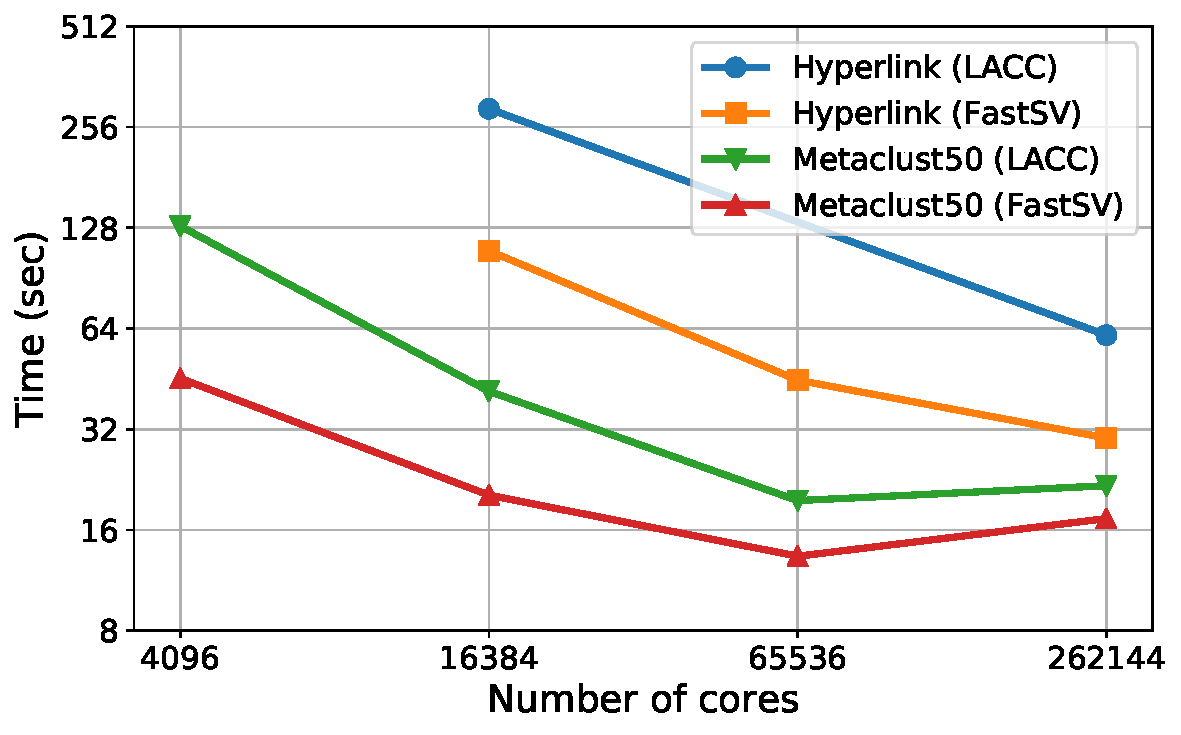
\includegraphics[width=0.65\textwidth]{figures/large-graph.pdf}
\vspace{-5pt}
\caption{Performance of \Name{} and LACC with two large graphs on CoriKNL (up to 262144 cores using 4096 nodes).}
\vspace{-10pt}
\label{fig:large}
\end{figure}

We separately analyze the performance of \Name{} and LACC on the two largest graphs in \autoref{tab:datasets}.
Hyperlink is perhaps the largest publicly available graph, making it the largest connectivity problem we can currently solve.
Since each of these two graphs requires more than 1TB memory, it may be impossible to process them on a typical shared-memory server.
\autoref{fig:large} shows the strong scaling of both algorithms and the better performance of \Name{}.
On the smaller graph Metaclust50, both algorithms scale to $65,536$ cores where \Name{} is $1.47\times$ faster than LACC.
On the Hyperlink graph containing 124.9 billion edges, they continue scaling to $262,144$ cores, where \Name{} achieves an $2.03\times$ speedup over the LACC algorithm.

%\subsection{Understand the performance of \Name{}.}

%In this section, we explore different features of \Name{} and discuss their potential impacts on its performance.

\begin{figure}[t]
\centering
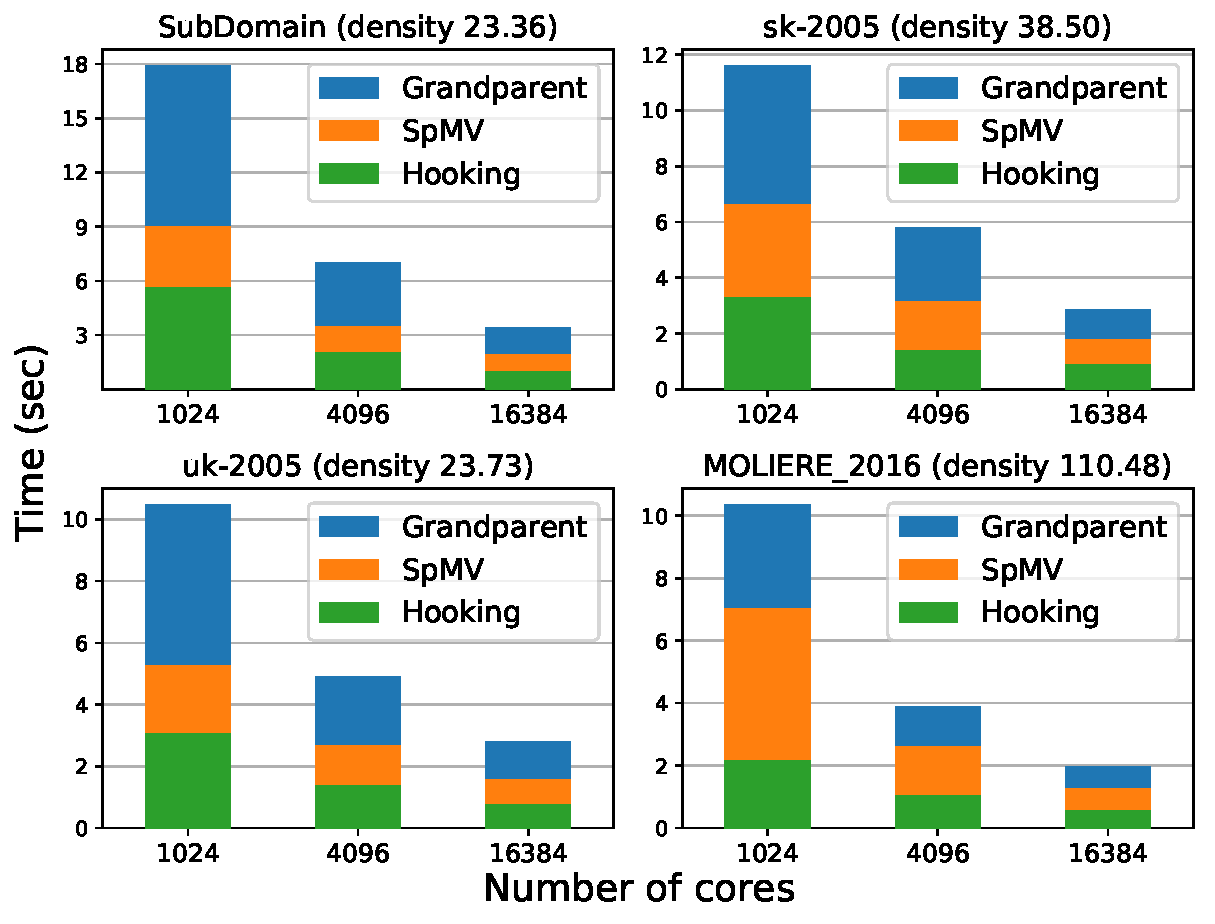
\includegraphics[width=0.8\textwidth]{figures/breakdown_sv_selected.pdf}
\vspace{-5pt}
\caption{Performance breakdown of \Name{} on four representative graphs.}
\vspace{-8pt}
\label{fig:sv-parts}
\end{figure}

\subsection{Performance characteristics}
\label{sec:breakdown}

In this subsection, we present more aspects of \Name{} to help readers understand the characteristics of this algorithm.

\textbf{Performance breakdown.}

%\textbf{Performance characteristics for each operation.}
%We first present the time spent on different phases of \Name{}.
\autoref{fig:sv-parts} shows the execution time of \Name{} by breaking the runtime into three parts: finding the grandparent, matrix-vector multiplication, the hooking operations.
The time spent on checking the termination is omitted, since it is insignificant relative to other operations.
% not even visible in our plotting.
% shows the results.
Each of these operations contributes significantly to the total execution time.
Finding the grandparent and the hooking operations basically reflect the parallel complexity of the \texttt{extract} and \texttt{assign} operations, and the ratio of them is relatively stable for all graphs.
By contrast, the execution time of SpMV varies considerably across different graphs, because SpMV's complexity depends on the density of a graph.

\begin{figure}[t]
\centering
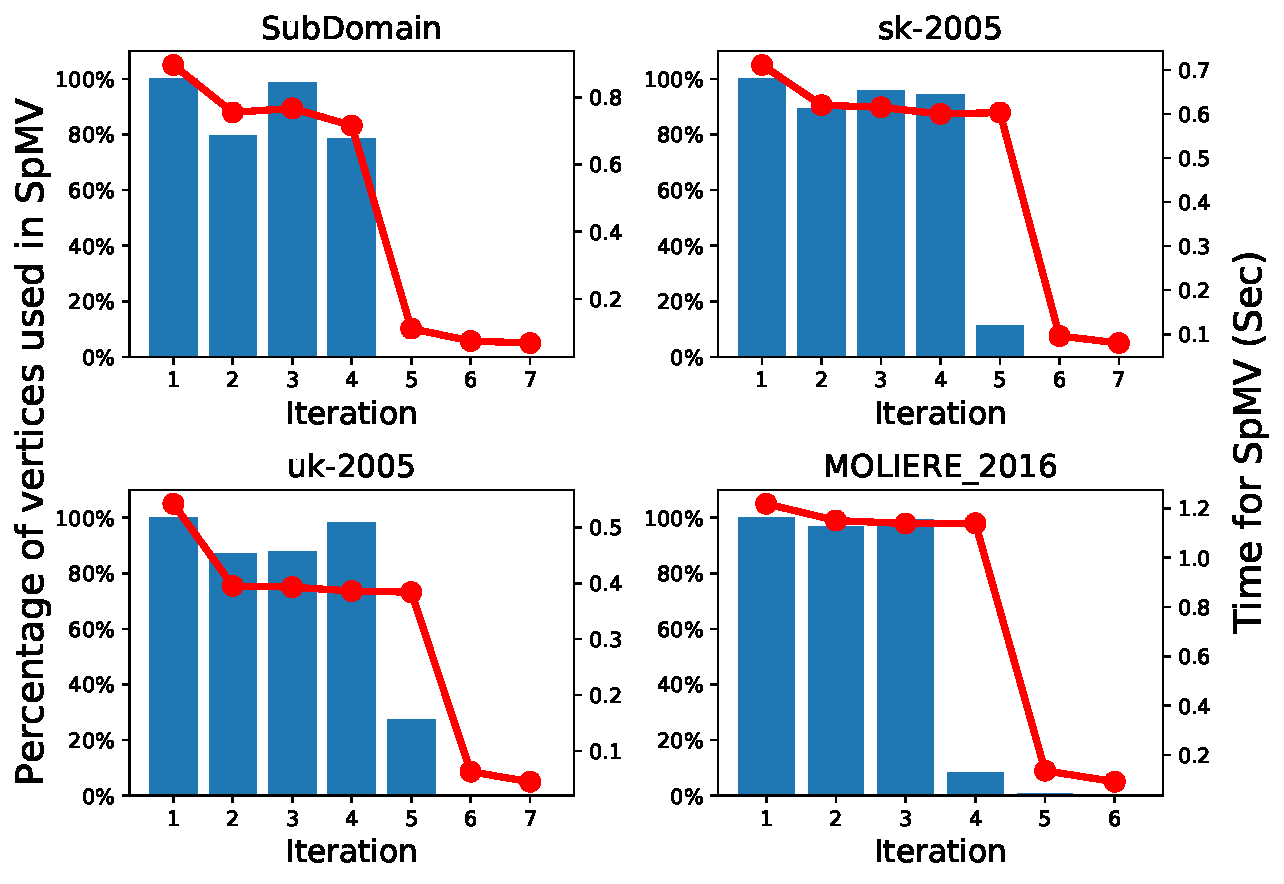
\includegraphics[width=0.75\textwidth]{figures/spmv-selected.pdf}
\vspace{-5pt}
\caption{Percentage of vertices that participate in the SpMV (sparse matrix-vector multiplication) operation for each iteration (bar chart), and the runtime for SpMV (line chart). A vertex participates the SpMV if its grandparent $\mathit{gf}$ is not changed in the previous iteration.}
\vspace{-10pt}
\label{fig:spmv-selected}
\end{figure}

\textbf{Execution time reduced by the sparsity optimization.}
\label{sec:sparsity}

As mentioned in ~\autoref{sec:sv-combblas}, \Name{} dynamically selects SpMV or SpMSpV based on the changes in the grandparent vector $\mathit{gf}$.
%use an adaptive way to perform the matrix-vector multiplication.
%If we find that most entries of the vector $\mathit{gf}$ are not modified in the previous iteration, we compute $\Delta\mathit{mngf}=\mathbf{A}\cdot\Delta\mathit{gf}$ instead of using the whole $\mathit{gf}$ in SpMV, to make use of the sparsity of $\Delta\mathit{gf}$ for reducing the computation time.
This optimization is particularly effective for high-density graphs where SpMV usually dominates the runtime (see  \autoref{fig:sv-parts}).
%can be justified by \autoref{fig:sv-parts} that for high-density graphs the time spent on SpMV is usually dominant.
\autoref{fig:spmv-selected} explains the benefit of sparsity with four representative graphs, where we plot the number of vertices modified in each iteration.
We observe that only a small fraction of vertices participates in the last few iterations where SpMSpV can be used instead of SpMV.
As shown by the red runtime lines in \autoref{fig:spmv-selected}, the use of SpMSpV drastically reduces the runtime of the last few iterations. 
% using the bar charts, whose curves show the typical cases that in the late iterations of \Name{}, there will be only a very small portion of the vertices modified in the graph.
%The number really depends on the structure of the graph.
%Then, we can see the effect of the sparsity optimization, where the time for performing the SpMV is significantly decreased when the number of modified entries is under some threshold.
%Note that the unmodified entries are not necessarily converged unless they did hook onto the smallest vertex in the connected component, while our algorithm is not able to detect it on the fly.

\section{Boruvka's algorithm}

\subsection{Vertex-centric \boruvka{}'s Algorithm}
\label{sec:boruvka}

\begin{figure}
\centering
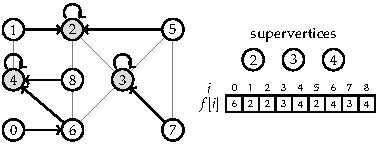
\includegraphics[width=0.75\textwidth]{figures/components.pdf}
\caption{Encode the currently recognized connected components of a graph as a vector. Each connected component has a unique identifier called \emph{supervertex}, and all the vertices connect to the supervertex through a direct link or a path.}
\vspace{-8pt}
\label{fig:components}
\end{figure}

\boruvka{}'s algorithm~\cite{boruvka} is considered the easiest for parallelization among the classic MSF algorithms~\cite{boruvka,kruskal,prim}.
Conventionally, its parallelization on distributed-memory is based on the Pregel~\cite{pregel} model where the computation is encoded as a \textit{vertex-program} that runs on every vertex and exchanges messages with the other vertex in a bulk synchronous way~\cite{bsp}.
\boruvka{}'s algorithm proceeds in rounds, and in each round, it picks a set of edges in a greedy manner and adds them to the final results.
The edges selected so far constitute a forest, in the edge of each round we contract the graph by removing the edges inside each tree.
The algorithm terminates when all the edges are removed.
It is worth noting that to quickly check whether an edge is connecting two vertices in the same tree or not, we encode all the spanning trees in a forest as a vector $f$, as shown in \autoref{fig:components}.
Each spanning tree elects a root vertex (a.k.a. \emph{supervertex}~\cite{salihoglu2014optimizing}), and the vector $f$ stores the parent vector for every vertex (the root points to itself). %vertex either points to the root directly or connects to the root through a directed path.
By flattening this structure, we have $f$ stores each vertex's supervertex so that we can easily tell whether two vertices are in the same spanning tree or not.
%To perform the edge removal, we need to quickly answer the queries whether two vertices belong to the same spanning tree or not.
%To achieve this, each spanning tree (or connected component) first elects a root vertex (a.k.a. \emph{supervertex}~\cite{salihoglu2014optimizing}), and then 
%Using this method, the connected components in the graph are encoded as a vector $f$, as shown in \autoref{fig:components}.

\boruvka{}'s algorithm starts with $n$ supervertices each containing a singe vertex.
In each round, we perform the following steps to construct the minimum spanning tree.
\begin{itemize}
\item \textbf{Min-edge picking:} each supervertex selects the minimum edge from the outgoing edges of all the vertices in the spanning tree.
This selected edge is then a candidate of the final result\footnote{The same edge might be picked by the supervertices of both endpoints. In this situation we only keep one of them and add it to the final result.}.
%If there are multiple edges having the same minimum weight, we just pick an arbitrary edge that connects to the tree with the smallest supervertex.
This procedure is further divided into two steps:
\begin{itemize}
\item \textbf{Step 1:} every vertex $u$ finds the minimum ordered pair $(w, f[v])$ for all $v$ in $u$'s adjacency list.
Then, $u$ sends the ordered pair along with the selected edge $(u, v)$ to $u$'s supervertex $f[u]$.
% for every edge $(u, v)$ in , and sends it to $u$'s root $f[u]$ along with the selected edge's information $(u, v)$.
\item \textbf{Step 2:} every supervertex then picks the minimum ordered pair $(w, f[v])$ among the received edges and changes its pointer to the supervertex $f[v]$.
If the spanning tree is isolated, the supervertex does nothing.
\end{itemize}
\item \textbf{Supervertex selection:} after the min-edge picking, the non-isolated supervertices in the graph will constitute a set of conjoined-trees~\cite{salihoglu2014optimizing}, each being a directed tree with a cycle of length two on the top.
We identify every such cycle $(u, v)$, select the smaller one of $u$ and $v$ as the new supervertex and make it a new root by creating a self-loop.
\item \textbf{Flattening:} every vertex $u$ finds the supervertex by repeatedly performing the shortcutting operation $f[u]\leftarrow f[f[u]]$ until the vector $f$ stabilizes.
\item \textbf{Edge cleaning:} remove the edges inside each tree, which are $(u, v)\in E$ having $f[u]=f[v]$.
%Recover the edges in the minimum spanning forest.
Repeat the above steps if there are still edges remained.
\end{itemize}

\autoref{fig:visualize} shows the MSF computation on a weighted graph using \boruvka{}'s algorithm.
%We present an example in  to show how it works for finding the MSF.
Starting from the input graph, every supervertex (which has no child in the first iteration) selects the minimum edge and the arrows form three conjoined-trees.
Then, the vertices 2, 3, 4 are selected as the new supervertices.
The flattening operation makes every vertex directly point to the new supervertex, and the edge cleaning removes the edges inside each spanning tree.
The graph is neither shrunk nor relabeled in order to maintain a low computation and communication cost.
%We do not shrink the connected component and relabel the edges, since it is an expensive operation on distributed-memory~\cite{salihoglu2014optimizing,yan2015effective}.
From the second iteration, the min-edge picking needs every supervertex to select the minimum outgoing edge from the whole spanning tree, and the result is shown in the lower left figure.
The other operations are similar to the first iteration, generating a spanning tree containing all the vertices in the graph.
The algorithm then terminates.
%In the lower right figure of \autoref{fig:visualize}, the supervertices 2, 3, 4 now point to each other while the rest vertices do not do anything.
%Vertex 2 picks the minimum edge $(5, 7)$ and points to vertex 3 which is the supervertex of vertex 7.
%The rest steps are not presented in the figure since they are similar to those in the first iteration.
%We can see that every vertex are now in the same connected component, so the algorithm terminates.
%Later we will see the detailed implementation of the min-edge picking using linear algebra operations \texttt{mxv} and \texttt{assign}.

\begin{figure}
\centering
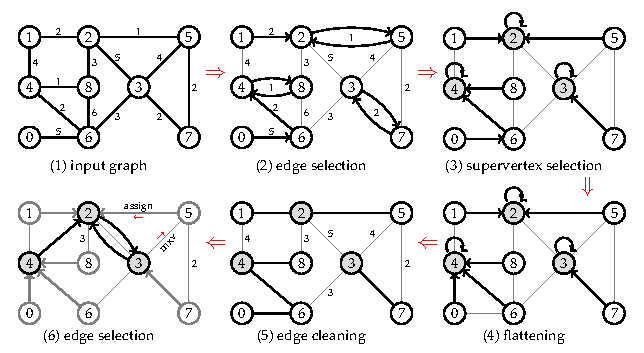
\includegraphics[width=\textwidth]{figures/algo.pdf}
\caption{The MSF computation using \boruvka{}'s algorithm, from the beginning to the min-edge picking in the second iteration. The arrows represent the parent vector $f$.}
\vspace{-8pt}
\label{fig:visualize}
\end{figure}

The primary issue affecting the distributed-memory performance in Pregel-like systems is the edge cleaning, which requires the predicate $f[u]=f[v]$ to be evaluated on every edge $(u, v)$.
In these systems, vector $f$ is an attribute associated on every vertex, and the evaluation of $f[u]=f[v]$ cannot be done without the message exchange if $u$ and $v$ are assigned to different physical nodes.
By assuming a random vertex assignment, the expected amount of messages to complete the edge cleaning is $O(E)$~\cite{bourse2014balanced}.
Our evaluation results show that it is a significant overhead in the MSF computation that takes up to $81.86\%$ of the total runtime (see \autoref{sec:performance}).

\subsection{A linear algebra formulation}
\label{sec:algorithm}

In this section, we express \boruvka{}'s algorithm in the language of linear algebra.
A commonly used linear-algebraic API for graph computation is the GraphBLAS C standard~\cite{graphblas}, but it is slightly verbose and hides the insights for distributed computing.
We therefore define a set of simplified APIs and then describe \boruvka{}'s algorithm in our framework.
%So, we first define a set of simplified APIs to describe \boruvka{}'s algorithm, and in \autoref{sec:impl} we will see how these operations are efficiently parallelized on distributed-memory.

%We store the input graph as a sparse adjacency matrix and use dense vectors in the whole algorithm, so the transformation from our simplified APIs to the GraphBLAS standard is straightforward.

In \autoref{algo:msf}, we present a step-by-step implementation for Borvuka's algorithm using the linear algebra APIs presented before.
The input is an undirected weighted graph represented as an adjacency matrix $\mathbf{A}$ and the output $\mathbf{MSF}$ is a submatrix of $\mathbf{A}$ containing the selected edges in the final minimum spanning forest.
%If we only care about the connected components, returning the vector $f$ is sufficient.

First of all, the min-edge picking is implemented on line 10--15, which aims to let every supervertex know (a) the minimum outgoing edge in the whole tree, including the edge weight and the supervertex id on the other side, and (b) the original edge in matrix $\mathbf{A}$ in order to recover the minimum spanning forest.
Most of the job is accomplished by the multiplication of $\mathbf{A}$ and $x$ shown in \autoref{fig:spmv}, and by combining the result $y$ with every $u$'s own vertex id, we obtain the vector $e_v$ containing the edge selected by every vertex.
%To achieve this, we first encode every vertex's minimum edge and the vertex's own id as a vector $x$, through the \texttt{mxv} operation shown in \autoref{fig:spmv}.
%The multiplication of $\mathbf{A}$ and $x$ computes
%The vector $x$ encodes each vertex's supervertex and its own id, %while the multiplication with the matrix $\mathbf{A}$ exactly computes the value we want.
Next, every supervertex collects the minimum edge from the whole spanning tree using the \texttt{assign} operation, and the idea of this operation is illustrated in \autoref{fig:assign} using a simplified example.
%So we compute a tuple $(w, f[v], u)$ for every supervetex $s$, and the such information is encoded as a vector $e_s$.
Finally, if $e_s[r]\neq \infty$ for a supervertex $r$, it modifies its entry in vector $f$ on line 15 using the second field in $e_s$.

\begin{comment}
The sparse-matrix multiplication let each vertex $u$ pick the minimum edge in its adjacency list.
The matrix value (edge weight) and the neighbor's supervertex id are first encoded into a pair using the \texttt{zip} function, and then the minimum pair is selected and stored on $u$, as shown in \autoref{fig:spmv}.
To send the selected pair to $u$'s parent, we use the \texttt{assign} function shown in \autoref{fig:assign}.
By providing a vector $f$ representing a flattened tree structure for each connected component, the \texttt{assign} operation let every root collect the minimum value in the whole tree.
Then, on line 10 -- 11, the root vertices that successfully selects an edge are the non-isolated supervertices of the previous iteration, and they extracts the index field (the second field) from the vector $\mathit{e_s}$.
\end{comment}

The supervertex selection on line 16--18 identifies the pairs of vertices $u$ and $v$ that point to each other ($f[u]=v$ and $f[v]=u$) and selects the smaller one as the new supervertex.
By a simple substitution, we need to find every $u$ having $f[f[u]]=u$ and let $u$ point to itself if $u<f[u]$.
The grandparent vector $f[f]$ is computed by the \texttt{extract} function and is stored in the vector $\mathit{g}$, then the following two \texttt{eWiseMult} operations compute all possible $u$'s and changes the pointer if the condition $u<f[u]$ is satisfied.

The flattening operation on line 21--25 is first performed on the old supervertices through the repetition of the shortcutting operation $f\leftarrow f[f]$ until stabilized.
This procedure takes at most $O(\log h)$ rounds where $h$ is the maximum height of all the spanning trees.
On line 25, all the vertices (which point to an old supervertex already) perform a single round of shortcutting to see the new supervertex.

The last step is the edge cleaning on line 27--33.
We first pick the edges in $\mathbf{A}$ that constitute the minimum spanning tree, by simply inspecting the vertices that become a non-supervertex in this iteration.
%The basic idea is that, the third field of $e_v$ stores the vertex who owns the selected edge.
Then, on line 28--31, we count the new supervertices (excluding the isolated supervertices in the previous step) and terminate the algorithm instantly if there is at most one active supervertices remained.
Next, by the \texttt{select} operation, we remove the edges inside each spanning tree and obtain a smaller matrix $\mathbf{A}$.
The algorithm terminates when $\mathbf{A}$ is empty.

\begin{algorithm}[t]
\caption{The linear algebra \boruvka{}'s algorithm for finding minimum spanning tree. \textbf{Input:} The adjacency matrix $\mathbf{A}$. \textbf{Output:} The matrix $\mathbf{MSF}$ containing the edges in the solution.}
\label{algo:msf}
\begin{algorithmic}[1]
\Procedure {BoruvkaMSF}{$\mathbf{A}$}
\State $\text{fill} (\mathit{super}, \mathbf{true})$ \Comment {non-isolated supervertex}
\State $\text{fill} (\mathit{inf}, \infty)$; $\text{fill} (\mathit{all}, \mathbf{true})$ \Comment {constant vectors}
\State $\text{fillWithIndex} (\mathit{ind})$ \Comment {vertex id (also a constant vector)}
\State $\text{fillWithIndex} (\mathit{f})$ \Comment {the initial parent vector}
\State $\mathbf{MSF} \leftarrow \emptyset$ \Comment {return value}
\Repeat
    \State $\text{copy} (\mathit{f'}, \mathit{all}, \mathit{f})$
    \State \Comment {Step 1: min-edge picking}
    \State $\text{eWiseMult} (\mathit{x}, \mathit{all}, \mathit{f}, \mathit{ind}, \text{zip})$ \Comment {$x[u]=(f[u],u)$}
    \State $\text{fill} (\mathit{y}, \infty)$; $\text{mxv} (\mathit{y}, \mathbf{A}, \mathit{x}, \text{zip}, \text{min})$
    \State $\text{eWiseMult} (\mathit{e_v}, \mathit{all}, \mathit{y}, \mathit{ind}, \text{zip})$ \Comment {$\mathit{e_v}[u]=(w, f[v], v, u)$}
    \State $\text{fill} (\mathit{e_s}, \infty)$; $\text{assign} (\mathit{e_s}, \mathit{super}, \mathit{f}, \mathit{e_v}, \text{min})$
    \State $\text{eWiseMult} (\mathit{super}, \mathit{all}, \mathit{e_s}, \mathit{inf}, \text{not\_equal\_to})$
    \State $\text{apply} (\mathit{f}, \mathit{super}, \mathit{e_s}, \text{second})$ %\Comment {\text{second field of} $\mathit{e_s}$}
    \State \Comment {Step 2: supervertex selection}
    \State $\text{extract} (\mathit{g}, \mathit{super}, \mathit{f}, \mathit{f}, \mathit{min})$
    \State $\text{eWiseMult} (\mathit{mask}, \mathit{all}, \mathit{g}, \mathit{ind}, \text{equal\_to})$
    \State $\text{eWiseMult} (\mathit{f}, \mathit{mask}, \mathit{f}, \mathit{ind}, \text{min})$
    %\State \Comment {update non-isolated supervertices}
    \State \Comment {Step 3: flattening}
    \State $\text{extract} (\mathit{g}, \mathit{super}, \mathit{f}, \mathit{f})$
    \While {$\mathit{f} \neq \mathit{g}$}
        \State $\text{copy} (\mathit{f}, \mathit{super}, \mathit{g})$
        \State $\text{extract} (\mathit{g}, \mathit{super}, \mathit{f}, \mathit{f})$
    \EndWhile
    \State $\text{extract} (\mathit{f}, \mathit{all}, \mathit{f}, \mathit{f})$
    \State \Comment {Step 4: edge cleaning}
    \State $\mathbf{MSF} \leftarrow \mathbf{MSF}~\cup~$\Call{RecoverMSF}{$\mathbf{A}, \mathit{f'}, \mathit{f}, \mathit{e_s}$}
    \State $\text{eWiseMult} (\mathit{mask}, \mathit{all}, \mathit{f}, \mathit{ind}, \text{equal\_to})$
    \State $\text{eWiseMult} (\mathit{super}, \mathit{all}, \mathit{super}, \mathit{mask}, \text{land})$
    \State $\text{reduce}(\mathit{active}, \mathit{all},\mathit{super}, \text{plus}, 0)$
    \State \textbf{if} $(\text{active}\leq 1)$ \textbf{then break}
    \State $\text{select} (\mathbf{A}, \mathbf{A}, \lambda(i,j,a_{ij})\rightarrow \{f[i]=f[j]\})$
    \State $\text{getNVals} (\text{nvals}, \mathbf{A})$
\Until {$\text{nvals}=0$}
\State \Return {$\mathbf{MSF}$}
\EndProcedure
\end{algorithmic}
\end{algorithm}

\begin{algorithm}[t]
\caption{The simplified edge picking operation in \boruvka{}'s algorithm for finding connected components.}
\label{algo:cc}
\begin{algorithmic}[1]
\Procedure {EdgePicking-CC}{$\ldots$}
    \State \Comment {$e_v$, $e_s$ are vectors of supervertex id}
    \State $\text{fill} (\mathit{e_v}, \infty)$; $\text{mxv} (\mathit{e_v}, \mathbf{A}, \mathit{f}, \text{second}, \text{min})$
    \State $\text{fill} (\mathit{e_s}, \infty)$; $\text{assign} (\mathit{e_s}, \mathit{super}, \mathit{f}, \mathit{e_v}, \text{min})$
    \State $\text{eWiseMult} (\mathit{super}, \mathit{all}, \mathit{e_s}, \mathit{inf}, \text{not\_equal\_to})$
    \State $\text{copy} (\mathit{f}, \mathit{super}, \mathit{e_s})$
\EndProcedure
\end{algorithmic}
\end{algorithm}

\begin{comment}
\State \Comment {Step 2.5: recover MSF edges}
\State $\text{eWiseMult} (\mathit{mask}, \mathit{all}, \mathit{f}, \mathit{ind}, \text{not\_equal\_to})$
\State $\text{fill} (\mathit{c}, \infty)$; $\text{apply} (\mathit{c}, \mathit{mask}, \mathit{e_s}, \text{second})$
\State $\text{extract} (\mathit{d}, \mathit{index}, \mathit{c})$
\State $\text{select} (\mathbf{T}, \mathbf{A}, \lambda(i,j,a_{ij})\rightarrow )$
\end{comment}


\subsection{A simplified algorithm for computing CCs}

\boruvka{}'s algorithm is capable of finding all the connected components in the graph, since each spanning tree is exactly a connected component, and the parent vector $f$ stores the component identifier for each vertex when terminated.
In order to make the CC computation more efficient, we can remove all the unnecessary computations in \autoref{algo:msf}.
The tree construction on line 27 is obviously useless.
Then, in the edge picking, we no longer take the edge weight into consideration, so the supervertices only collects the smallest neighboring supervertex id from the whole tree.
We give a reference implementation in \autoref{algo:cc}.

\subsection{The guarantee of convergence}
\label{sec:convergence}

\boruvka{}'s algorithm terminates in $\log(n)$ rounds in the worst case for both MSF and CC computation.
Consider the number of non-isolated spanning trees in the graph.
Initially, this number is $n$, and in each round after the min-edge picking, all the non-isolated supervertices constitute a set of conjoined-trees, and only one vertex in each conjoined-tree will become a new supervertex in the next round.
A conjoined-tree has at least two vertices, so the number of new supervertices (including both isolated and non-isolated ones) is at most half of the number of non-isolated supervertices in the previous round.
In practice, this algorithm converges very fast.
\autoref{sec:msf-eval} presents more detailed results for different types of graphs.
A very useful corollary is that the accumulated number of non-isolated supervertices during the whole computation is $O(n)$.

\section{Implementation}

%\subsection{Implementation of FastSV in linear algebra}

%In this section, we first give the formal description of FastSV in GraphBLAS, a standardized set of linear algebra primitives for describing graph algorithms.
%We then present its linear algebra distributed-memory implementation in Combinatorial BLAS~\cite{combblas} and discuss two optimization techniques for improving its performance.

%In this section, we formally define the semantics of FastSV using GraphBLAS~\cite{graphblas}, 
%We choose GraphBLAS API due to its conciseness, and it also implies a distributed-memory implementation in CombBLAS~\cite{combblas}, a framework for large-scale graph processing in linear algebra.


\subsection{Data placement for matrix and vector}
\label{sec:basic-op}

%When launching a graph computation task, multiple processes are launched, each .
The graph is represented as an $n$-by-$n$ symmetric matrix $\mathbf{A}$ representing the adjacency relationship of the vertices.
We split the matrix by column and let each process store a whole vertical strip, as shown in \autoref{fig:spmat}.
% where each element $a_{ij}$ of matrix $\mathbf{A}$ represents and edge from vertex $i$ to vertex $j$ with an integer edge weight $a_{ij}$.
We assume that the vertices are indexed with $0..n-1$ where $n$ is the total number of vertices.
Then, the elements stored on each process are the edges having the destination vertex in a disjoint range of $[0..n-1]$.
We randomly permute the indices to obtain a good load balancing.

For each vector, it is either fully distributed on all the processes such that each process holds a disjoint segment with roughly the same number of elements, or simply replicated on all the processes.
The replication of a vector obviously has higher memory consumption, but we consider it viable since the number of vertices in a practical graph can typically fit into the main-memory, and for some operations (like the flattening operation we will discuss later), only in this representation it can be finished in reasonable time.
Choosing the most suitable representation for each vector used in \boruvka{}'s algorithm is important to achieve high performance.

%For a vector, it can be either distributed on all the processes such that each process holds a disjoint segment with roughly the same number of elements, or can be just replicated on all the processes.
%In \autoref{fig:spmat}, the gray part shows
%The later option obviously has larger memory consumption, but 
%In our framework, there are two alternatives to store a vector on the cluster.
%One way is to fully distribute the vector on all the processes so that each process holds a disjoint segment with roughly the same number of elements.
%The other way is to replicate the vector on all the processes so that each process sees all the contents of the vector.
%This method is memory-efficient but each process sees incomplete information of the whole vector.
%Suppose we launch $p$ processes for a graph computation, this representation obviously has $p\times$ higher memory consumption.
%In practice, we can assume that each computation node is large enough to hold all the vertices of a graph, and $O(m/n)$ is the maximum number of processes required to store all the edges of a graph.
%Then, $p\leq m/n$ is a reasonable assumption

\subsection{Overview of the implementation}

In this thesis, we implement all our linear algebraic operations using two levels of data parallelism, one is MPI for inter-node communication and the other is OpenMP for multithreading on each node.
We mainly discuss the following operations, \texttt{mxv}, \texttt{assign} and \texttt{select}, since the others are essentially element-wise operations that can be easily parallelized.
We also give a special implementation of the flattening operation (which iteratively performs the \texttt{extract} operation), which makes use of the vertex replications to avoid the high communication cost.
%In addition, there is a special low-level operation \texttt{replicate} in our implementation that converts a vector's distributed store to the replicated store.
%We also have a special implementation of the flattening operation based on a property of \boruvka{}'s algorithm to further reduce its computation cost.

In our implementation, we replicate as few vectors as possible to minimize the memory consumption.
Essentially, only the vector $\mathit{f}$ and $\mathit{e_s}$ in \autoref{fig:spmat} need to be replicated on all the processes, and it is basically an requirement for implementing the \texttt{mxv} and \texttt{assgin} operations.
For the constant vectors (such as $\mathit{inf}$, $\mathit{all}$ and $\mathit{ind}$) and the intermediate vectors $\mathit{x}$ and $\mathit{g}$, even though they are involved in the element-wise computations with $\mathit{f}$, in our implementation, we compute them on the fly so that the actual storage is not necessary.
%For all the other vectors, each process only stores an aligned disjoint segment in the local memory so that element-wise operations can be trivially parallelized.

\subsection{Parallelization of the linear algebra operations}

In this subsections, we go through the parallel implementation for all the aforementioned linear algebra operations.
\begin{itemize}
\item \texttt{mxv}: this is the key linear algebra operation in many graph computations.
In our model, the multiplication $y=x\mathbf{A}^T$ (or equivalently $y=\mathbf{A}x$ since we do not distinguish a vector with its transpose) is accomplished by replicating the vector $x$ on every process and computing a distributed vector $y$.
Each element of $y$ is obtained by a process computing the inner product of $x$ and the corresponding column in $\mathbf{A}^T$ using the user-specified operators $\oplus$ and $\otimes$.
We store the matrix $\mathbf{A}^T$ in the compressed sparse column (CSC) format so that the OpenMP parallelism is straightforward.
%On each process, we further split the matrix $\mathit{A}^T$ into smaller strips and store each of them using the compressed sparse row (CSR), so that the thread-level parallelization is achieved by an assignment of the strips to the threads.
%The use of OpenMP for \texttt{mxv} is trivial by spliting the matrix $$
%There is no communication cost at all and the computation cost is $O(m)$.
%Such computation can be easily parallelized by OpenMP.

%\item \texttt{replicate}: a vector can be stored in the form of either a distributed vector or a replicated vector during the computation.
%The replication is simply achieved by the master thread on each process sending the local segment to all the processes through the \texttt{MPI\_Allgatherv} function.
%Depending on the sparsity of the vector, we can either broadcast the whole vector or only the nonzero elements.

%\item \textbf{Conversion between the two representations}: a vector can be stored in the form of either a distributed vector or a replicated vector during the computation, and the conversion between the two representations is a basic operation in our model. The direction from the replicated store to the distributed store is trivial, while for the opposite direction each process broadcasts its own segment to the whole process world. Depending on the sparsity of the vector, we can either broadcast the whole vector or only the nonzero elements.

% since each process just extracts the segment from the replicated vector according to its rank.
%In opposite, from the distributed store to the replicated store, each process needs to broadcast its own segment to the whole process world, requiring a total amount of $O(np)$ messages transfered from one process to another.

%\item \textbf{Synchronization of the replicated vector}: in our model, a vector can be replicated on the process world. In this case, each process can modify its local entries independently, but at some point we need to synchronize the replicas so that all MPI processes can agree on the same result. This is accomplished by the \texttt{MPI\_Allreduce()} function on the entries modified by at least one process through a user-specified binary operation.
%, which takes $O(Lp\log(p))$ messages where $L$ is the number of entries that are actually synchronized.

\item \texttt{assign}: this is the key operation to let every supervertex collect the information from all the vertices in the spanning tree.
Our implementation is presented in \autoref{fig:assign-impl} where the output vector $\mathit{y}$ is the only vector that is initially replicated on all the processes.
To accomplish the \texttt{assign} operation, each process first performs the local computation that modifies its own replica of $\mathit{y}$ using OpenMP and atomic writes, then all the processes synchronize the modified entries in $\mathit{y}$.
For the synchronization, the sparse vector \texttt{super}, playing the role of the mask of \texttt{assign}, is replicated on all the processes through the \texttt{MPI\_Allgatherv} function, and then the specified entries in $\mathit{y}$ are extracted and synchronized through the \texttt{MPI\_Allreduce} function.

%\item \texttt{extract}: this is the dual operation of \texttt{assign}.
%Similar to element-wise operations, this operation can be easily parallelized on both 
%In our implementation of \boruvka{}'s algorithm, both the input and output vectors are replicated on all the processes, so we simply perform a local computation on each process, and it can be trivially parallelized by OpenMP since there is no conflict writes.

\item \texttt{flattening}: the flattening operation (line 21--24 of \autoref{algo:msf}) is an iterative procedure that performs the \texttt{extract} operation repeatedly to half the distance from every vertex in $\mathit{super}$ to the root.
Here the boolean vector $\mathit{super}$ contains the old supervertices generated in the previous iteration.
The overall computation cost reaches $O(np)$ (see the analysis in \autoref{sec:cost}) but the communication cost is completely removed, making it an efficient solution on small clusters.
%This particular implementation has an overall $O(np)$ computation cost but gets rid of the hard-to-parallel communication cost.
%In \autoref{sec:cost}, we justify our choice by proving an overall $O(np)$ computation cost.

\begin{comment}
this operation is described by an iterative procedure using the \texttt{extract} function, as described on line 20--23 of \autoref{algo:msf}.
Slightly different from the straightforward implementation of \texttt{extract} described above, in the flattening operation, we extract the indices of the mask $\mathit{super}$ in advance and then perform the \texttt{extract} operation on the extracted indices to avoid the unnecessary scan on the whole vector.
\end{comment}

\item \texttt{select}: in \boruvka{}'s algorithm, this operation removes the edges $(u, v)\in E$ having $f[u]=f[v]$.
Due to the replication of the vector $f$ on all the processes, the \texttt{select} operation can inspect the supervertex of both $u$ and $v$ without incurring any communication cost.
We implement this operation by a single-pass scan on every edge, and we allow a vertex $u$ to keep different neighbors belonging to the same connected component, so that an $O(E)$ computation cost can be ensured.
The \texttt{mxv} operation is implemented with \texttt{select} to maximize the performance.
%The parallelization is achieved by assigning CSR blocks to the threads, which is the same as the \texttt{mxv}.
%We actually combine the \texttt{select} with \texttt{mxv} to maximize the performance.
\end{itemize}

%The sparse matrix-vector multiplication (SpMV) is the key operation in graph computations.
%In our implementation, the partitioning of the sparse matrix follows the 2D block decomposition\cite{kumar1994}, as shown in FIGURE.
%We distribute the sparse matrix on a $\sqrt{p}\times \sqrt{p}$ processor grid where $P(i, j)$ stores the submatrix $A_{ij}$ of dimensions $(m/\sqrt{p})\times(m/\sqrt{p})$ in its local memory.

\begin{figure}
\centering
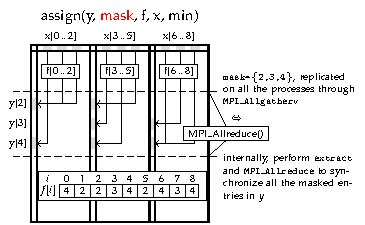
\includegraphics[width=0.8\textwidth]{figures/assign-impl.pdf}
\caption{The implementation of the \emph{assign} operation in our model. Each process sees a disjoint portion of the input vectors $x$, $f$ and $\mathit{mask}$. Then, it computes and stores the partial results to the replicated vector $y$. We first replicate the vector $\mathit{mask}$ using MPI's all-gather function, then all the processes synchronize the union of the modified entries in $y$ (indicated by the parameter $\mathit{mask}$) by MPI's all-reduce function.}
\vspace{-8pt}
\label{fig:assign-impl}
\end{figure}

\begin{comment}
In the rest of this section, we will go through all the operations used in \autoref{algo:msf} to see which vertex are replicated and how each operation is implemented.

\subsection{Min-edge picking}
\label{sec:assign}

The min-edge picking operation consists of two key operations, the matrix-vector multiplication \texttt{mxv} to pick the minimum edge from every vertex's adjacency list, and the \texttt{assign} operation to aggregate the minimum edge to the supervertex.
The \texttt{mxv} operation, as mentioned before, is a basic operation in our framework.

The subvector assign and extract are the dual operations to exchange information between the vertices in each connected component, as illustrated in \autoref{fig:assign}.

For both operations, we store the index vector $f$ in a fully distributed way.
We first need to decide how the input and output vectors are distributed on the cluster.
\autoref{fig:assign-impl} is our solution, in which we always store $f$ in a fully distributed way, then the input vector $x$ is aligned with $f$ and the output vector $y$ is replicated on every process.
The \texttt{assign} operation is actually simple to implement where each process simply modifies the entries in $y$ on its own replicate, and then synchronize the results across the processes.

The synchronization requires an additional vector $\mathit{mask}$, which specifies all the entries in $y$ that are modified by at least one process.
In \boruvka{}'s CC algorithm, this vector is exactly the set of non-isolated supervertices in each iteration, or the vector $\mathit{super}$ in \autoref{algo:msf}.
We fully distribute the boolean vector $\mathit{super}$ on all process and update it via element-wise local computations, but at the beginning of each iteration, we broadcast the nonzero indices of vector $\mathit{super}$ to every process, which is the mask given to the \texttt{assign} function.
The total amount of non-isolated supervertices during the whole MSF computation is $O(n)$ according to our analysis in \autoref{sec:boruvka}, making the \texttt{assign} operation efficient in communication cost.
We note that the rest entries in $y$ are undefined, and during the MSF computation we will never read or write those locations.

\subsection{Maintaining the non-isolated supervertices}

Maintaining the non-isolated supervertices is an important step in our implementation of \boruvka{}'s algorithm, which keeps a low complexity for various operations.
For example, the assign operation mentioned before needs to know in advance how many supervertices are modified across all the processes in each iteration.
We use a simple method to track the non-isolated supervertices during the computation.

The computation is based on the following observations:
\begin{itemize}
\item All the supervertices point to itself at the beginning of each iteration.
\item In the min-edge picking, the isolated supervertices do nothing but the non-isolated supervertices points to some other vertices.
\end{itemize}
Then the non-isolated supervertices are the intersection of the supervertices at the beginning of the iteration, and the vertices that do not point to itself after the min-edge picking.

In our implementation, each process XXX.


\subsection{Iterative subvector extract for flattening}

The flattening operation is described by an iterative procedure using the \texttt{extract} function, as described in \autoref{algo:msf}.
An interesting result is that, our implementation has $O(np\log(n))$ computation cost with a total amount of $O(np)$ messages for the whole MSF computation regardless of the number of iterations each flattening operation takes or the number of rounds the \boruvka{}'s algorithm takes.

Our solution is based on an important property of \boruvka{}'s algorithm that the number of non-isolated supervertices during the whole computation is $O(n)$.
%We know that for the rest vertices in the graph, it is either in an isolated spanning tree where there is no need to change anything, or a leaf node pointing to a non-isolated supervertex.
Therefore, our strategy is to first perform the iterative \texttt{extract} operation on the set of non-isolated supervertices, and then perform a single round of shortcutting operation $f[u]=f[f[u]]$ on all the vertices.

It consists of the following three steps:
\begin{itemize}
\item Each process extracts the non-isolated supervertices and broadcast them to all the processes.
\item Each process then performs local computation to identify the root of all the non-isolated supervertices, by iteratively doing the shortcutting operation $F[u]\leftarrow F[F[u]]$ in parallel.
\item After every non-isolated supervertex finds the root, every other vertex performs a single round of shortcutting operation $F[u]\leftarrow F[F[u]]$ in parallel to identify the new supervertex.
\end{itemize}

It is easy to see that the total number of non-isolated supervertices during the whole MSF computation is at most $n+n/2+\ldots+1$, which is less than $2n$.
This is the only data communication in the flattening operation.
For the same reason, the comptation cost for the second step is $O(n\log(n))$ where $n$ is the total number of non-isolated vertices in all iterations and $log(n)$ is the number of iterations the flattening operations takes for finding the supervertex.
The last step takes a constant $O(n)$ time in each iteration, the complexity is $O(n\log(n))$ during the whole computation since \boruvka{}'s algorithm terminates in $\log(n)$ rounds.


\subsection{Submatrix selection for edge cleaning}

The last operation is the \texttt{select} operation that removes the edges $(u, v)\in E$ having $f[u]=f[v]$.
We know that every process has obtained the latest $f$ after the flattening operation.
Then, it is obvious that if we have vector $f$ replicated on every process, this operation can be done by scanning the CSR structure exactly once without incurring any communication cost.
From the implementation of the iterative \texttt{extract} operation, we can see that every process indeed computes the whole vector $f$.
The \texttt{select} function has an upper-bound of $O(E)$ computation cost.
To make this operation efficient, we do not merge the parallel edges, so a vertex $u$ may keep different $v$'s belonging to the same connected component $f[v]$.

\end{comment}

\subsection{Cost Analysis}
\label{sec:cost}

In the end of this section, we analyze the total computation and communication cost for our implementation of \boruvka{}'s algorithm.
We use $n$ and $m$ to represent the number of vertices and edges in the graph, and use $p$ to represent the number of processes.
The algorithm terminates in $O(\log n)$ rounds.
%We use $n$ and $m$ to represent the number of vertices and edges in the graph, $r$ to represent the number of iterations (which is $O(\log n)$ but can be much smaller in practice) and $p$ to represent the number of processes.

\begin{comment}
\begin{table}
\caption{Total computation and communication cost for each operation in \boruvka{}'s algorithm.}
\label{tab:cost}
\begin{tabular}{c|c|c}
\hline
operation & computation & communication \\
\hline
\texttt{mxv} & $O(mr)$ & 0 \\
\hline
\texttt{assign} & $O(pnr)$ & $O(pn)$ \\
\hline
\texttt{extract} & $O(pnr)$ & 0 \\
\hline
\texttt{flattening} & $O(pn\log n)$ & 0 \\
\hline
\texttt{select} & $O(mr)$ & 0 \\
\hline
\end{tabular}
\end{table}
\end{comment}

First, the only communication cost in our implementation is the \texttt{assign} operation where the vertices sends their selected edges to the supervertex.
The total communication cost, as illustrated in \autoref{fig:assign-impl}, is the cost of performing an \texttt{MPI\_Allgather} to replicate the mask on all the processes plus an \texttt{MPI\_Allreduce} to synchronize the values of the supervertices.
We know that the accumulated number of supervertices during the whole computation is $O(n)$ (see \autoref{sec:convergence}), so the \texttt{assign} operation requires $O(np)$ messages in total for both operations.

For all the other operations, there is no communication cost at all.
In each iteration, \texttt{mxv} and \texttt{select} take $O(m)$ time, and all the element-wise operations, depending on whether the vector is replicated or not, takes either $O(np)$ or $O(n)$ time where $p$ is the replication factor.
Note that an $O(np)$ time complexity can be very huge if we unrestrainedly increase the number of processes $p$ for the CC or MSF computation.
In order to achieve high performance, we use as few processes as possible in practice to reduce the computation cost.
We assume $M>n$ where $M$ is the memory space of a single node, and using at most $p=O(m/n)$ physical nodes the graph can fit into the main-memory of the cluster.


%The above two operations already have an $O((m+pn)\log n)$ time complexity in total.
For the flattening operation, in each \boruvka{} round, every process individually performs the subgraph flattening (line 21--24) which scans the supervertices only by at most $O(\log n)$ times.
The overall time complexity is $O(pn\log n)$ where $n$ is the accumulated number of supervertices during the whole computation, $p$ is the replication factor.
By summing up all the numbers above, \boruvka{}'s algorithm has an $O((m+pn)\log n)$ computation cost and $O(np)$ communication cost.
In particular, when $p=1$, there is actually no communication cost, and our parallel implementation for \boruvka{}'s algorithm achieves the optimal $O(m\log n)$ time complexity.


\begin{comment}
\autoref{tab:cost} shows communication for each operation during the whole MSF computation.
The analysis of the communication cost of \texttt{assign} is a little bit complicated.
The first operation bringing communication cost is the replication of the mask, which is the vector $\mathit{super}$ in \autoref{algo:msf} representing the current non-isolated supervertices.
An important property of \boruvka{}'s algorithm is that the number of non-isolated supervertices is at least halved after each iteration, so the total number of non-isolated supervertices cannot exceed $2n$ and the replication cost is $O((p-1)n)$ in total.
The all-reduce operation in MPI is also performed on the non-isolated supervertices and thus has the same communication cost $O((p-1)n)$.
The analysis of the \texttt{flattening} is similar.
The iterative procedure restrained on all non-isolated supervertices gives it an $O(pn\log n)$ computation cost where $O(\log n)$ is the expected number of rounds to converge in each iteration.

By summing up the results above, the total computation cost is $O((m+pn)\log n)$ and the total communication cost is $O((p-1)n)$.
Note that for a vertex-centric implementation, the communication cost alone is $O(m\log n)$ due to the edge cleaning in a hash-based vertex partition.
In most real-world graphs, $n$ is one or two order of magnitude smaller than $m$, making or implementation much more message-efficient than a vertex-centric implementation.
\end{comment}

\begin{table}[t]
\centering
\caption{Graph datasets used to evaluate the parallel CC and MSF algorithms.}
\vspace{-5pt}
\footnotesize
\label{tab:gap-matrices}
\begin{tabular}{lrrHl}
\hline
Graph & Vertices & Edges & Components & Description \\
\hline
GAP-road & 23.95M & 57.71M & 1 & the distances of all of the roads in the USA~\cite{gap-road} \\
GAP-twitter & 61.58M & 2.937B & 19926186 & a crawl of Twitter's social network in 2009~\cite{gap-twitter} \\
GAP-web & 50.64M & 3.861B & 123 & a web crawl of .sk domain in 2005~\cite{davis2011university} \\
GAP-kron & 134.2M & 4.223B & 71164263 & a graph synthesized by the Kronecker synthetic graph generator~\cite{gap-kron} \\
GAP-urand & 134.2M & 4.295B & 1 & a graph synthesized by the Erdos–Reyni model (Uniform Random)~\cite{gap-urand} \\
\hline
\end{tabular}
\end{table}

\begin{figure}[t]
\centering
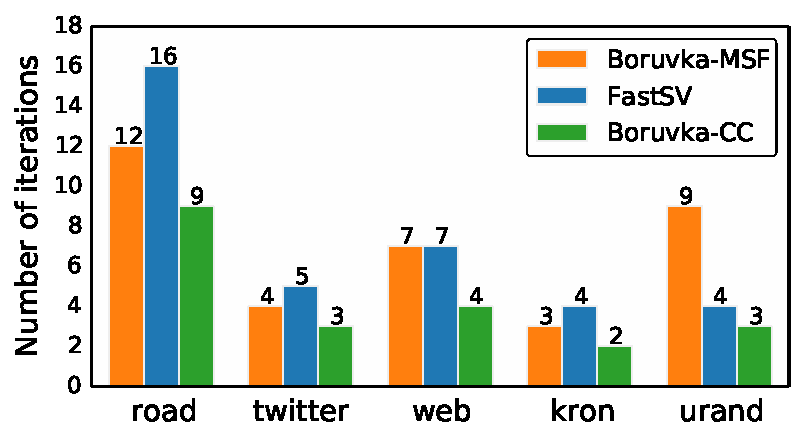
\includegraphics[width=0.6\textwidth]{figures/iterations.pdf}
\caption{Number of iterations \boruvka{}'s algorithm and FastSV take on the graphs in the GAP benchmark.}
\vspace{-8pt}
\label{fig:iterations}
\end{figure}

\section{Evaluation of \boruvka{}'s algorithm}
\label{sec:msf-eval}

In this section, we evaluate various aspects of our linear algebraic \boruvka{}'s algorithm, including the speed of convergence, distributed-memory performance, scalability and several other performance characteristics.
To make a fair comparison with previous works, we target the minimum spanning forest problem and the connected component problem separately, and our solution for solving each problem is named as \boruvka{}-CC and \boruvka{}-MSF, respectively.
\boruvka{}-CC is basically a simplification of \boruvka{}-MSF that only reports the number of connected components, ignoring the edge weight and the construction of the minimum spanning tree.

For the minimum spanning forest problem, \boruvka{}'s algorithm is currently the only algorithm parallelized on the distributed-memory architecture, and previous works~\cite{yan2014pregel,zhang2019composing} all adopt the vertex-centric paradigm.
We compare our linear algebraic \boruvka{}-MSF with Pregel-channel~\cite{zhang2019composing}'s implementation, which reports the fastest runtime compared to previous works.
There are more distributed-memory algorithms~\cite{hashmin,parconnect,lacc,fastsv} proposed for distributed-memory architecture in various models, and we compared our \boruvka{}-CC with FastSV~\cite{fastsv}, which is currently the fastest and the most scalable algorithm using the linear algebra abstraction.

We use the GAP benchmark matrices~\cite{gap-benchmark} (summarized in \autoref{tab:gap-matrices}) to evaluate these implementations, which include both synthetic and real-world weighted graphs of different types.

\subsection{Evaluation platform}

We evaluate the distributed-memory algorithms on Amazon EC2.
Our implementation is compared against two libraries, CombBLAS~\cite{combblas} and Pregel-channel~\cite{zhang2019composing}.
CombBLAS use both MPI and OpenMP to parallelize the graph algorithms, but it adopts a different partitioning strategy that the matrix is decomposed in a two-dimensional way and the vectors are fully distributed on all the processes using a range-based manner.
Pregel-channel is parallelized with MPI only, in which the vertices are distributed to all the processes in a hash-based manner and the edges are associated on the source vertex.
 % and for both programs, only the main thread will make MPI calls.
%CombBLAS is parallelized with MPI and OpenMP, but we execute it in pure MPI mode to maximize its performance.
%Given $p$ processes, CombBLAS always organizes them into a square $\sqrt{p}\times\sqrt{p}$ process grid and each MPI process stores a subgraph of the input matrix.
%Pregel-channel is parallelized by MPI. The vertices are distributed to the processes through a hash function and the edges are attached to the source vertex.
All these implementations follow the Bulk Synchronous Parallel (BSP)~\cite{bsp} model where all MPI processes perform local computation followed by synchronized communication round.
We set up a cluster of eight nodes with 10Gbps network bandwidth, and each node is an r5.4xlarge instance having 16 vCPUs and 128G memory.
This is the minimum configuration for the CombBLAS library in terms of memory space.
We compile all the programs using g++ 7.4.0 with -O3 flag.

\begin{comment}
\begin{table}
\caption{Basic characteristics of the graph analytics libraries used in our evaluation.}
\label{tab:libraries}
\footnotesize
\begin{tabular}{l|l|l}
\hline
Graph Library  & Parallelism & Matrix Distribution \\
\hline
CombBLAS & MPI + OpenMP & 2D~/~range-based \\
\hline
Pregel-Channel & pure MPI & 1D~/~hash-based \\
\hline
\boruvka{}-CC/MSF & MPI + OpenMP & 1D~/~range-based \\
\hline
\end{tabular}
\end{table}
\end{comment}

\subsection{Speed of convergence}

We first look at the speed of convergence of the \boruvka{}-CC and the FastSV algorithm.
FastSV's design is based on the PRAM Shiloach-Vishkin algorithm~\cite{ShVi82} with various optimizations to improve its convergence on distributed-memory architecture.
Then, \autoref{fig:iterations} clearly shows that \boruvka{}-CC takes less number of iterations than FastSV on all our five graphs.
The number of iterations does not directly reflect the performance since the complexity of each iteration matters, but later we will see the high efficiency of \boruvka{}'s algorithm's each iteration as well.
Then, computing the minimum spanning tree using \boruvka{}'s algorithm generally takes more iterations, and the main reason is the different edge picking strategy of \boruvka{}-MSF that takes the edge weight into consideration.
There is also a vertex-centric implementation of \boruvka{}'s algorithm in the vertex-centric paradigm, and we should not that it takes exactly the same number of iterations as \boruvka{}-MSF, since the algorithm is deterministic and the implementation methods will not affect its convergence.

%The flattening operation for finding the supervertex is an iterative procedure performing the subvector extraction operations, each of which will incur some communication cost in CombBLAS's model since each MPI process can only see a segment of the whole vector.
%Our implementation use less MPI process and let each process holds the whole vector, therefore making the flattening a complete local computation.

%In this subsection, we compare the distributed-memory performance and many other aspects of the simplified \boruvka{}'s algorithm, or we call \boruvka{}-CC, with the state-of-the-art FastSV~\cite{fastsv} algorithm for distributed-memory.

\subsection{Distributed-memory performance}
\label{sec:performance}

Next, we evaluate the distributed-memory performance of our algorithms in solving the connected component and the minimum spanning forest problems.
The experiment is conducted on a cluster of eight nodes using 64 cores in total.

\begin{comment}
\begin{figure}[t]
\centering
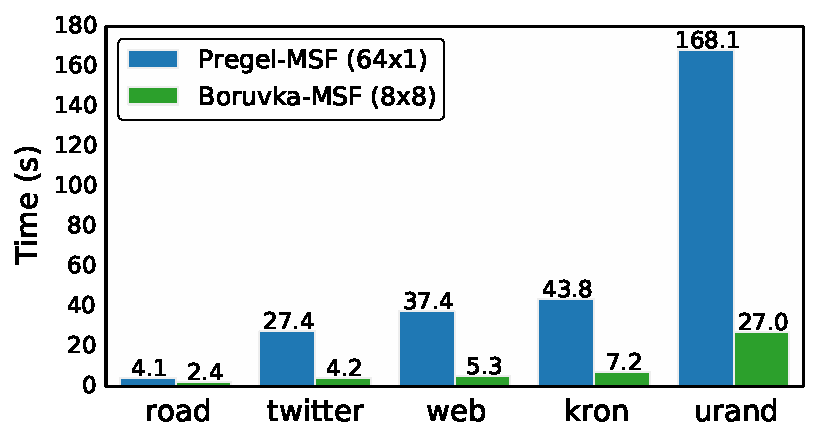
\includegraphics[width=0.40\textwidth]{figures/MSF-time.pdf}
\caption{Runtime of \boruvka{}'s MSF algorithm on the graphs in the GAP benchmark.}
\vspace{-8pt}
\label{fig:time-msf}
\end{figure}


\begin{figure}[t]
\centering
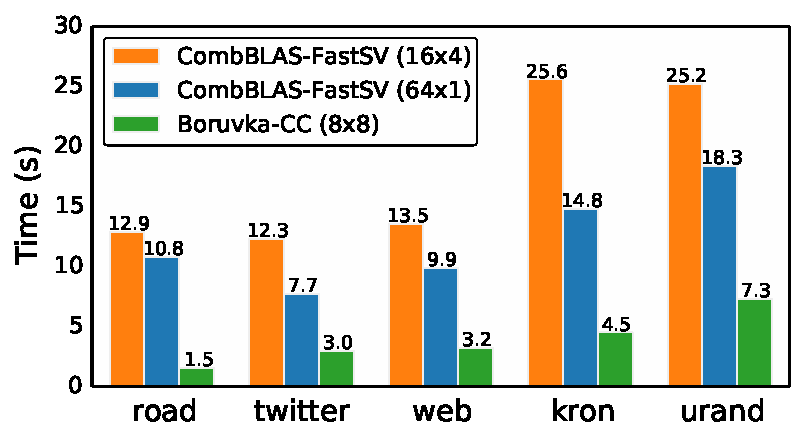
\includegraphics[width=0.40\textwidth]{figures/CC-time.pdf}
\caption{Runtime of FastSV and \boruvka{}-CC on the five graphs in the GAP benchmark.}
\vspace{-8pt}
\label{fig:time-cc}
\end{figure}
\end{comment}

\begin{figure}[t]
\centering
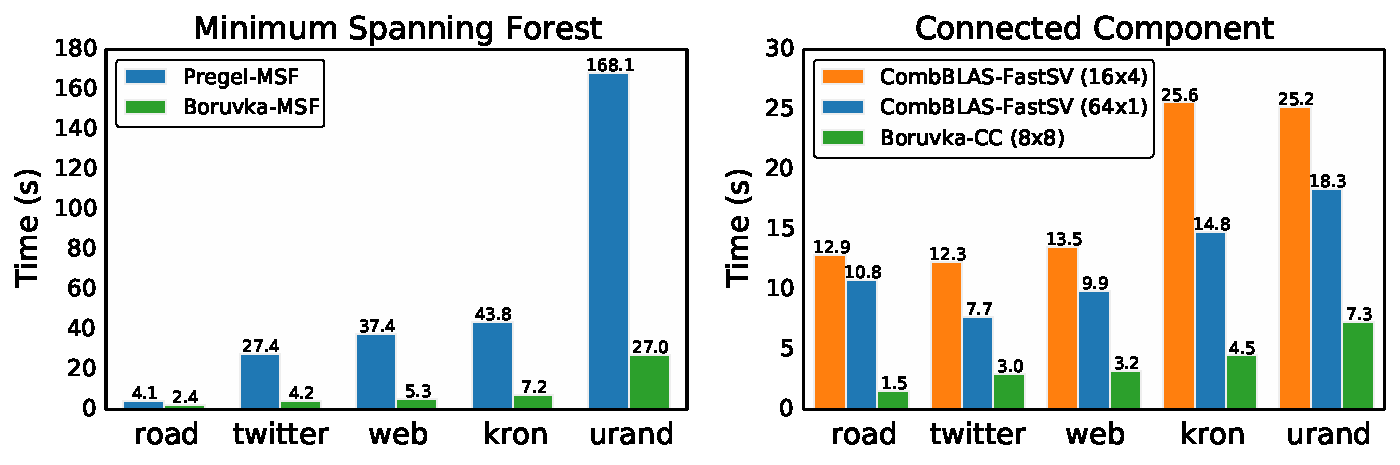
\includegraphics[width=0.9\textwidth]{figures/runtime.pdf}
\caption{Runtime of \boruvka{}'s algorithm on the five graphs in the GAP benchmark.}
\vspace{-8pt}
\label{fig:runtime}
\end{figure}

\textbf{Minimum spanning forest.}
We first compare the runtime of \boruvka{}'s MSF algorithm's vertex-centric implementation with our linear algebraic implementation.
We use Pregel-channel's implementation~\cite{zhang2019composing} of \boruvka{}'s algorithm due to its channel mechanism to reduce the message size and the higher performance reported in the paper compared to the previous works.
Pregel-channel's main functionality runs in the pure MPI mode, so we launch 64 MPI processes to make full use of the CPU cores.
For our \boruvka{}-MSF implementation in linear algebra, we launch 8 MPI processes, one for each node, each using 8 threads for its local computation.
\autoref{fig:runtime} presents the results on the five graphs in the GAP benchmark.

Compared to Pregel-channel's vertex-centric implementation, our linear algebraic implementation achieves a speedup of $1.75\times$ on the road graph and a speedup of $6.09\times$ to $7.03\times$ on the other four graphs.
Our implementation of \boruvka{}'s algorithm has a factor of $p$ (the number of processes) for element-wise operations on replicated vectors.
Therefore, on the planner road graph with high sparsity, our approach is not remarkably better than a vertex-centric implementation.
However, for the other graphs where $|E|$ is one or two magnitude larger than $|V|$, we can see that the linear algebraic approach is significantly faster, and the reason is our efficient implementation of the \texttt{select} operation that incurs no communication cost at all.
%By using the replicated vectors, the \texttt{select} function can see the attributes associated on both endpoints.
%On the contrary, in Pregel's vertex-centric model, each vertex removes an edge after it knows which connected component its neighbor belongs to, which has to be achieved by message passing.
We note that the percentage of time spent on the edge cleaning operation in Pregel reaches $75.13\%$ to $81.86\%$ on the last four graphs (except the road graph), proving that the edge cleaning is a very heavy operation in the vertex-centric model.
On average\footnote{The averaged speedup is the ratio of the total time spent on all the graphs in the GAP benchmark by the two programs.}, our linear algebra implementation achieves a $6.10\times$ speedup on all the graphs in the GAP benchmark.

\textbf{Connected component.}
We then compare the runtime of FastSV and \boruvka{}-CC for finding the connected components in each graph.
FastSV is implemented in CombBLAS~\cite{combblas} using its linear algebra primitives while the CombBLAS is parallelized by MPI and OpenMP.
CombBLAS's implementation requires the number of MPI processes $p$ to be a square number so that the matrix is divided into $\sqrt{p}\times\sqrt{p}$ submatrices and is evenly distributed to the process grid.
We therefore run CombBLAS's FastSV program in two configurations, one with 64 MPI processes each having 1 thread, and the other with 16 MPI processes each having 4 threads.
\autoref{fig:runtime} presents the results on the five graphs in the GAP benchmark.

The linear algebra \boruvka{}-CC is clearly faster than FastSV's both runs on all instances.
For FastSV, running it in the pure MPI mode is faster than the hybrid MPI+OpenMP mode in CombBLAS.
Compared to FastSV's best result using 64 processes, our \boruvka{}-CC achieves a speedup of $6.98\times$ on the road graph, and it is $2.53\times$ to $3.29\times$ faster on the other graphs.
We have already seen that \boruvka{}-CC converges faster than FastSV, but even if we compare the runtime of each iteration, \boruvka{}-CC is still $3.20\times$ faster on the road graph and is $1.56\times$ to $1.89\times$ on the other graphs, due to our slightly better \texttt{mxv} and much better implementation of the \texttt{extract} and \texttt{assign} operation.
We present a detailed analysis in \autoref{sec:characteristics}.
On average, \boruvka{}-CC is $3.16\times$ faster than FastSV on all the graphs in the GAP benchmark using 8 nodes and in total 64 threads.
%\boruvka{}-CC converges faster than FastSV, but if we look at the averaged runtime for each iteration in \autoref{fig:cc-per-iter}, \boruvka{}-CC is still $3.43\times$ faster on the road graph and is $1.65\times$ to $2.00\times$ on the rest graphs.
%We should note that, CombBLAS, as a linear algebraic library, also suffers the problem of high computation cost on sparse graphs like the road graph, and its implementation of the \texttt{assign} function is even slower.
%In all the graphs except the road graph, we observe that the matrix-vector multiplication spends most of the time during the execution.

\subsection{Performance characteristics}
\label{sec:characteristics}

In this subsection, we present more aspects of \boruvka{}'s algorithm to help readers understand the strategies used in our distributed-memory implementation.

\begin{figure}[t]
\centering
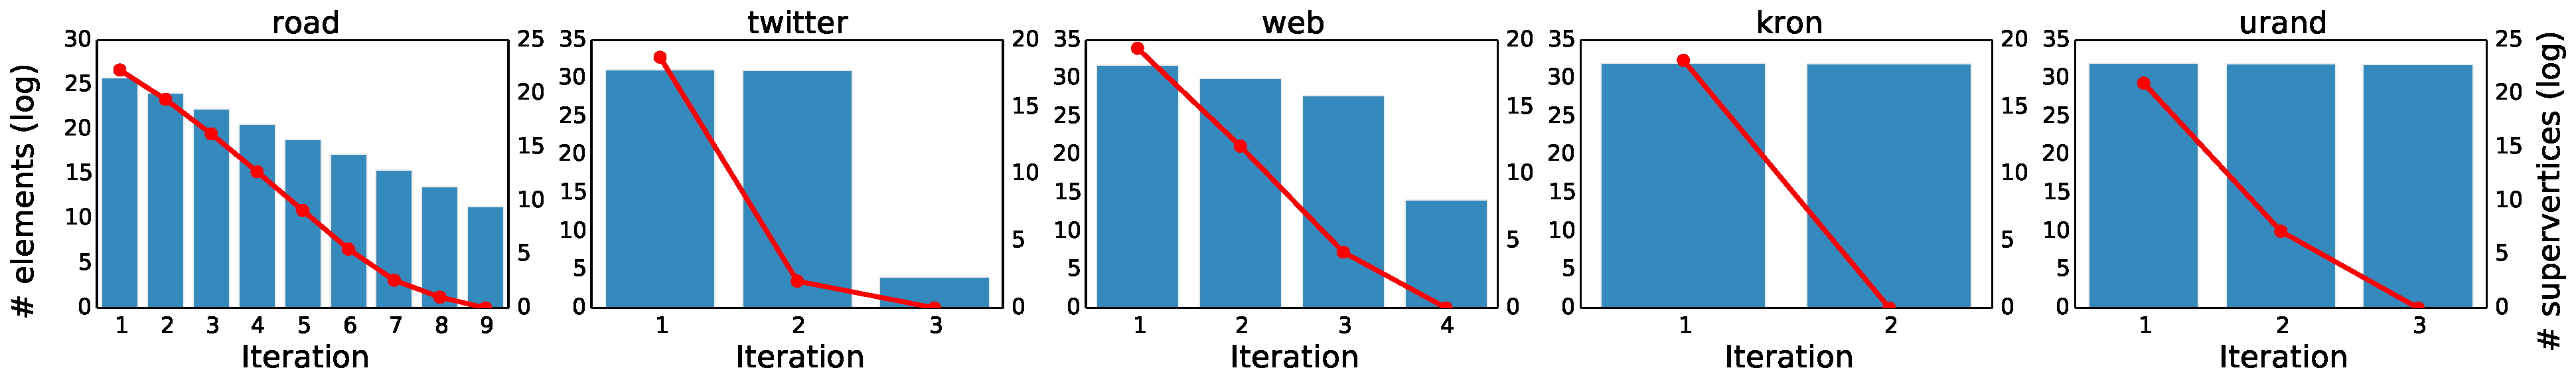
\includegraphics[width=\textwidth]{figures/iter-active-CC.pdf}
\caption{Number of elements in the matrix at the beginning of each iteration (bar chart) and the number of newly selected supervertices in each iteration (line chart) for \boruvka{}-CC.}
\vspace{-8pt}
\label{fig:active-cc}
\end{figure}

\begin{figure}[t]
\centering
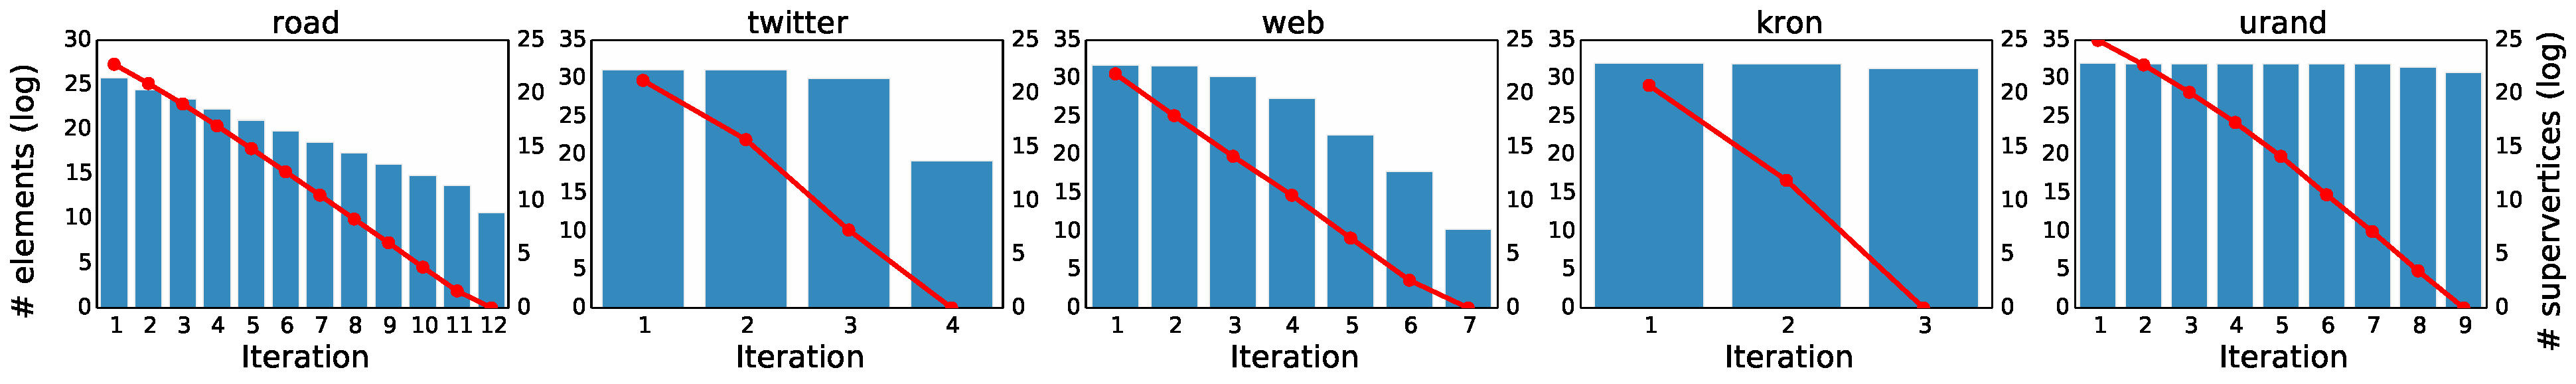
\includegraphics[width=\textwidth]{figures/iter-active-MSF.pdf}
\vspace{-8pt}
\caption{Number of elements in the matrix at the beginning of each iteration (bar chart) and the number of newly selected supervertices in each iteration (line chart) for \boruvka{}-MSF.}
\vspace{-8pt}
\label{fig:active-msf}
\end{figure}

\begin{figure}[t]
\centering
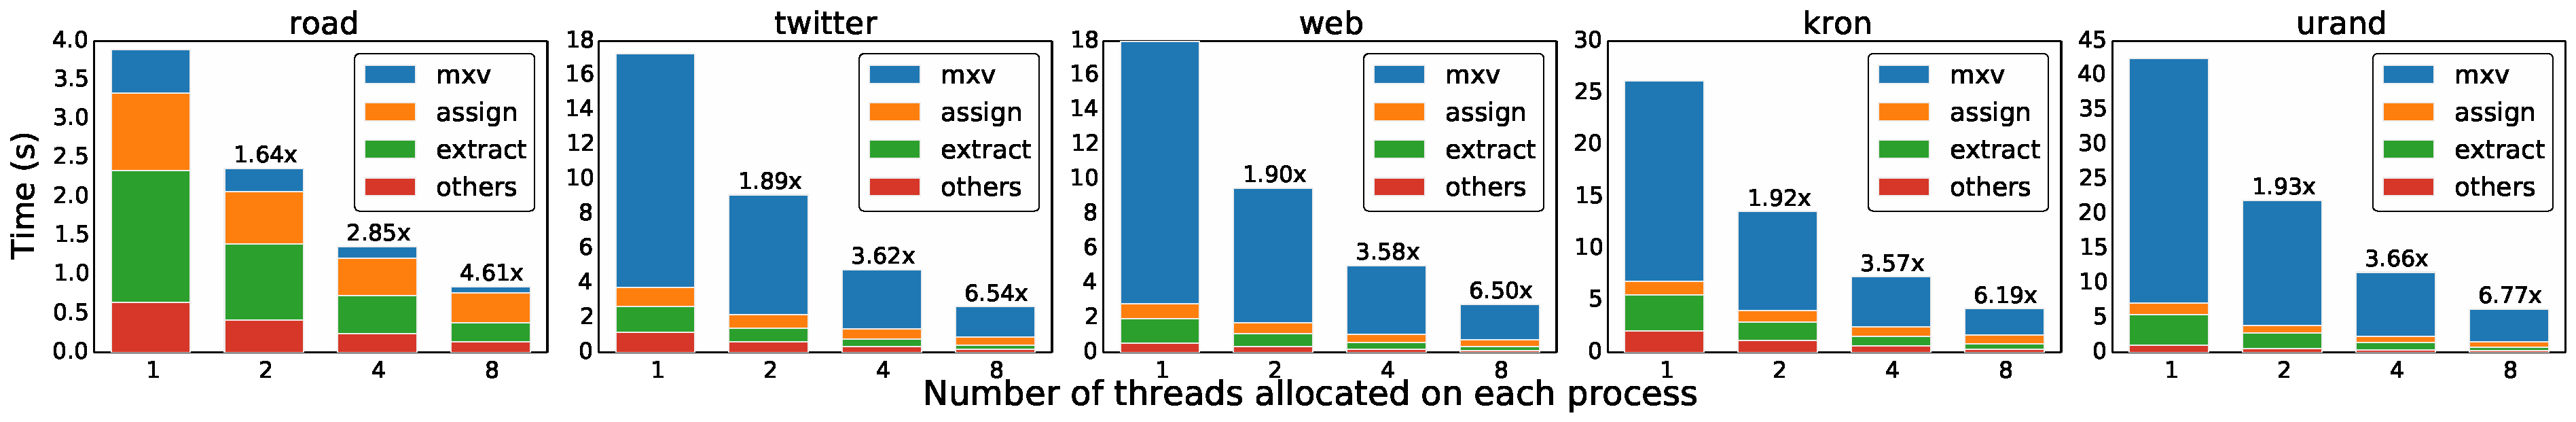
\includegraphics[width=\textwidth]{figures/CC-runtime-breakdown.pdf}
\vspace{-8pt}
\caption{Breakdown of the runtime for \boruvka{}-CC on eight nodes using different number of threads.}
\vspace{-8pt}
\label{fig:breakdown-cc}
\end{figure}

\begin{figure}[t]
\centering
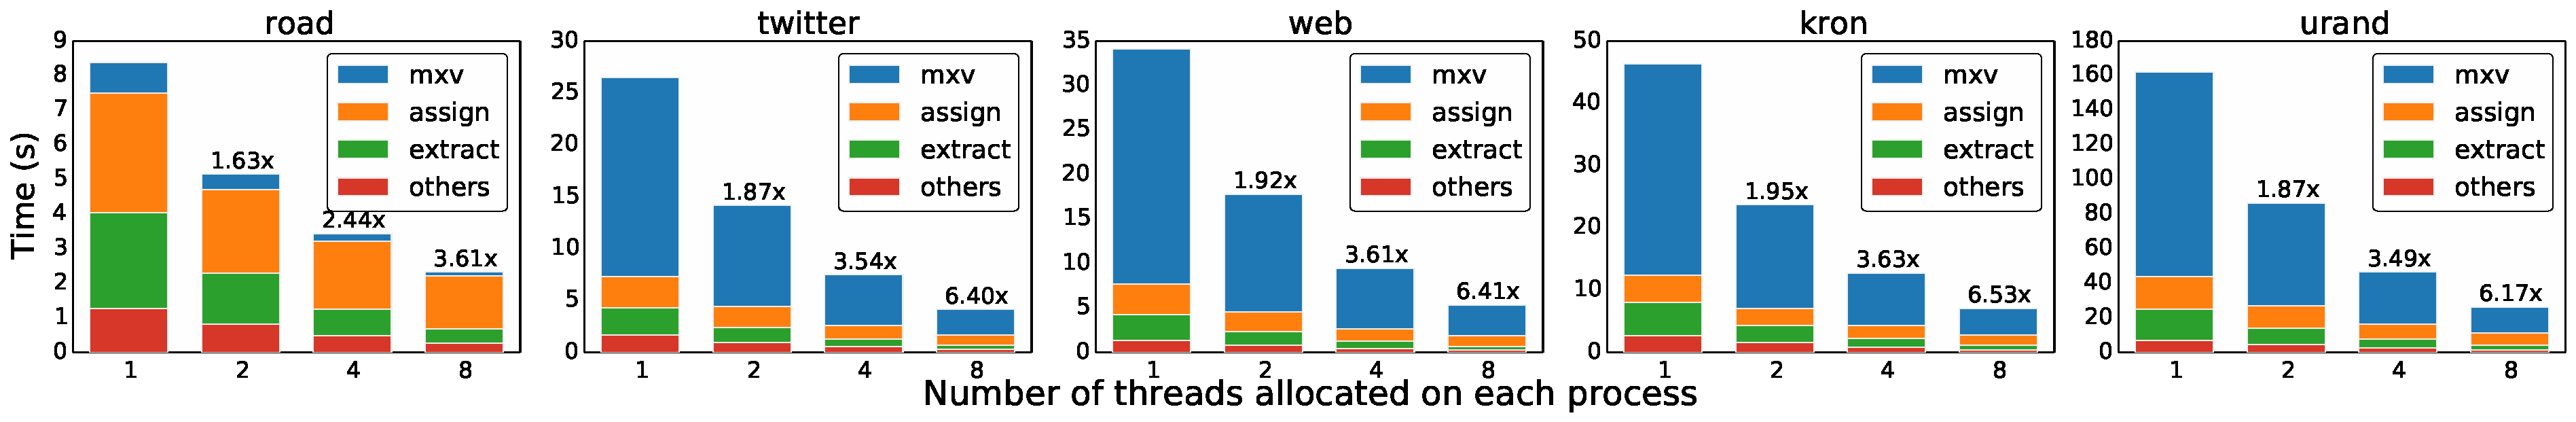
\includegraphics[width=\textwidth]{figures/MSF-runtime-breakdown.pdf}
\caption{Breakdown of the runtime for \boruvka{}-MSF on eight nodes using different number of threads.}
\vspace{-8pt}
\label{fig:breakdown-msf}
\end{figure}

\textbf{Active edges and supervertices}.
In \autoref{fig:active-cc} and \autoref{fig:active-msf}, we plot the number of active edges and supervertices during the execution of \boruvka{}-CC and \boruvka{}-MSF.
The active edges are the edges remained in the graph in the end of each iteration, meaning that they are currently connecting different spanning trees in the spanning forest constructed so far.
Then, the active supervertices are the newly selected supervertices in each iteration, which decides the communication cost of the \texttt{assign} operation.
We use bar chart and line chart respectively to represent the active edges and supervertices and both numbers are presented in log scale.

%From the figure, we can see how fast the graph shrinks when running \boruvka{}'s algorithm.
The number of active supervertices, as expected, decreases rapidly with the execution of \boruvka{}-MSF and \boruvka{}-CC.
The accumulated number during the whole computation (except the first iteration that all vertices are supervertices), as shown in \autoref{tab:num-roots}, varies from $0.28\%$ to $23.92\%$ for \boruvka{}-CC and $1.35\%$ to $41.25\%$ for \boruvka{}-MSF on different types of graphs.
It reflects the actual communication cost of the \texttt{assign} operation.

On the contrary, the number of active edges in each iteration may not notably decrease during the computation.
On the two synthetic graphs kron and urand, even in the last iteration, the number of edges removed is less than $4\%$.
Therefore, in the worst case, \boruvka{}'s algorithm has an average $O(E)$ edges in the matrix during the whole computation.
A vertex-centric implementation therefore needs $O(E)$ messages to perform the \texttt{select} operation in every iteration, while in our linear algebraic implementation there is no communication at all.
We have already seen that the edge cleaning can take up to $81.86\%$ percentage of the total execution time in a Pregel implementation.
%For the road and web graph, the runtime of the \texttt{mxv} takes much less in the late iterations.

\begin{table}
\centering
\caption{Accumulated number of active supervertices during the whole computation of the \boruvka{}'s algorithm for CC and MSF, presented in the ratio to the graph size $n$.}
\label{tab:num-roots}
\vspace{-8pt}
\begin{tabular}{c|c|c|c|c|c}
\hline
algorithm & road & twitter & web & kron & urand \\
\hline
\boruvka{}-CC & 23.92\% & 0.71\% & 1.38\% & 0.28\% & 1.56\% \\
\boruvka{}-MSF & 41.25\% & 4.14\% & 8.09\% & 1.35\% & 31.05\% \\
\hline
\end{tabular}
\vspace{-4pt}
\end{table}

\begin{figure}
\centering
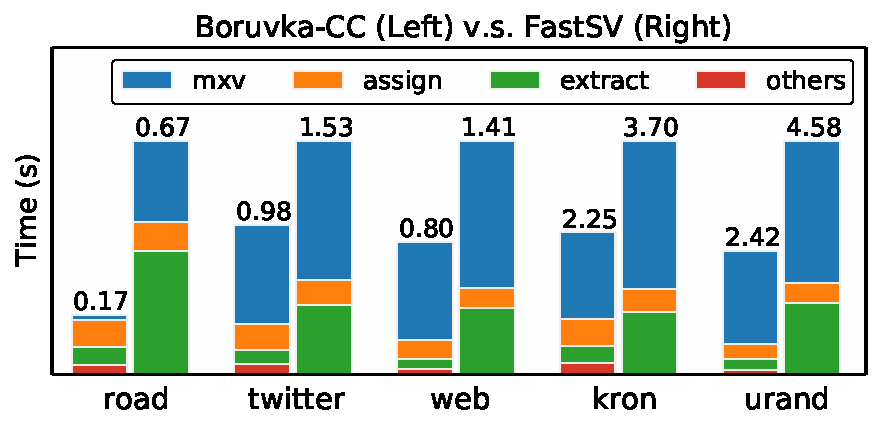
\includegraphics[width=0.6\textwidth]{figures/CC-breakdown.pdf}
\caption{Per-iteration runtime for each type of linear algebra operations in \boruvka{}-CC and FastSV.}
\vspace{-10pt}
\label{fig:breakdown}
\end{figure}

\begin{comment}
\begin{table}
\caption{Per-iteration runtime for each operation used in \boruvka{}-CC and FastSV \todo{use figure}.}
\label{tab:breakdown}
\vspace{-8pt}
\begin{tabular}{|c|c|c|c|c|c|c|c|c|c|c|}
\hline
\multirow{2}{*}{operation} & \multicolumn{2}{c|}{road} & \multicolumn{2}{c|}{twitter} & \multicolumn{2}{c|}{web} & \multicolumn{2}{c|}{kron} & \multicolumn{2}{c|}{urand} \\ 
\cline{2-11}
 & \boruvka{} & FastSV & \boruvka{} & FastSV & \boruvka{} & FastSV & \boruvka{} & FastSV & \boruvka{} & FastSV \\
\hline
mxv & 0.1384 & 0.2258 & 0.8340 & 0.8396 & 0.7582 & 0.8209 & 1.8753 & 2.1775 & 2.8701 & 2.5105\\
\hline
assign & 0.0310 & 0.0804 & 0.0421 & 0.1506 & 0.0375 & 0.1114 & 0.0783 & 0.3443 & 0.0845 & 0.3433\\
\hline
extract & 0.0256 & 0.3421 & 0.0682 & 0.4156 & 0.0413 & 0.3711 & 0.2231 & 0.9075 & 0.1580 & 1.2517\\
\hline
others & 0.0146 & 0.0000 & 0.0604 & 0.0000 & 0.0268 & 0.0000 & 0.1576 & 0.0100 & 0.0728 & 0.0100\\
\hline
\end{tabular}
\end{table}
\end{comment}

\textbf{Scalability and performance breakdown.}
To see the scalability of \boruvka{}'s algorithm, we change the number of threads each process can use in the CC and MSF computation.
The total number of processes is still 8 since we have 8 nodes in the cluster.
We break down the runtime of \boruvka{}'s algorithm into four parts, the matrix-vector multiplication along with the \texttt{select} operation (they are combined into a single operation), the \texttt{assign}, the \texttt{extract} and all the other operations.
\autoref{fig:breakdown-cc} and \autoref{fig:breakdown-msf} presents our results.

The overall speedup with the OpenMP parallelism using 8 threads achieves more than $6\times$ for both \boruvka{}-CC and \boruvka{}-MSF on the four dense graphs. %, and most parts scale very well, except for the \texttt{assign} operation which has a constant $O(np)$ communication cost.
The \texttt{mxv} dominates the runtime and achieves the highest speedup (more than $7.5\times$ on average), while \texttt{assign} has the lowest speedup (around 2-3$\times$) due to the constant communication cost.
The \texttt{extract} and the others are element-wise operations and scale as well as \texttt{mxv}.
%The runtime of the \texttt{extract} operation, or more precisely the flattening operation consisting of several rounds of \texttt{extract}, takes only a small portion of the total runtime of \boruvka{}-CC on all experiment settings.
%However, even for a single \texttt{extract} operation in FastSV's each iteration, the execution time is huge and .
%Depending on the graph (but except the road graph since it is too sparse), this number is always between $4\%$ and $10\%$ for both algorithms, and is lower for denser graphs.
%According to \autoref{tab:num-roots}, \boruvka{}-MSF has much more non-isolated vertices during the computation than \boruvka{}-CC, which increases its overall communication cost.
%The last part in red is the runtime of element-wise operations to determine the new supervertices, which takes the least amount of time.

%FastSV's implementation also relies on the \texttt{assign} and \texttt{extract} operations, but our \boruvka{}-CC's implementation of these two operations are more efficient.
\autoref{fig:breakdown} shows the per-iteration time spent on each operation for \boruvka{}-CC and FastSV.
On average, \boruvka{}-CC's \texttt{mxv} is $1.66\times$ faster and \texttt{assgin} is equally fast, but the \texttt{extract} function (or more precisely the iterative \texttt{extract} in flattening) is $5.51\times$ faster than FastSV.
%In particular, we can see that the \texttt{extract} operation takes a big portion of the total runtime of FastSV, making its each iteration more expensive than \boruvka{}-CC.
The main reason is the removal of the communication cost of the \texttt{extract} operations in our implementation. %, which is restrained by the number of active supervertices (see \autoref{sec:cost}).
For the \texttt{mxv} operation, \boruvka{}'s algorithm pays additional cost for the \texttt{select} operation, but on graphs like road and web, the cost of \texttt{mxv} decreases dramatically in later iterations.

%The main reason for this result is that, the overall cost of \boruvka{}'s \texttt{extract} and \texttt{assign} is much lower .


%FastSV's \texttt{extract} implementation incurs high communication cost due to the skewed communication pattern, but \boruvka{}-CC implements the \texttt{extract} using only local computation.

%Clearly, our \texttt{assign} and \texttt{extract} takes much less time.

%For the extract operation, our implementation does not incur any communication cost but only needs some additional local computation.
%For the assign operation, the total amount of communication is actually quite small compared to the number of vertices, as presented in \autoref{tab:non-roots}.
%For the \texttt{mxv} operation, both algorithms has advantages.
%\boruvka{}-CC's runtime is mainly affected by the graph size in each iteration, but FastSV's \texttt{mxv} operation is quite stable.

\section{Related work}

%\todo{sequential, parallel} how to present???
Finding the minimum spanning tree (or forest) in an undirected weight graph is a well-studied problem in sequential or on shared-memory.
The classic sequential algorithms given by \boruvka{}~\cite{boruvka}, Prim~\cite{prim} and Kruskal~\cite{kruskal} provide $O(m\log n)$ time complexity.
Some algorithms~\cite{yao1975,cheriton1976finding,osipov2009filter,chazelle2000minimum,gabow1986efficient,pettie1999finding} have theoretically lower time complexity, but they are either hard to parallelize or not efficient on practical graphs due to a big hidden factor.
On multiprocessors or shared-memory systems,
%Among the classic algorithms, \boruvka{}'s algorithm is considered the easiest for parallelization. %, since Kruskal's algorithm relies on the parallel sorting and Prim's algorithm is essentially sequential in its edge picking step.
Bader's work~\cite{bader2006fast} presents a new MST algorithm that combines the idea of Prim's and \boruvka{}'s algorithm, and several recent works on parallelizing \boruvka{}'s algorithm include~\cite{pingali2011tao,da2015generic,zhou2017practical} exploits various issues on shared-memory, including the graph representation, cache effect and the load balancing.
%All these solutions are generally similar to our shared-memory solution (by degrading the algorithm )
%There solutions are generally similar to our shared-memory version (by degrading my algorithm to one node), but they do not indicate a distributed-implementation at all.
%In general, these solutions are similar, 
Our work focuses on reducing the communication cost on distributed-memory, but on shared-memory, it also has the optimal time complexity $O(m\log n)$ and we demonstrate its high scalability in our evaluation.

On distributed-memory, \boruvka{}'s algorithm has been parallelized and implemented in several Pregel-like systems~\cite{salihoglu2013gps,yan2014pregel,zhang2019composing}.
Pregel~\cite{pregel} stands for a particular type of vertex-centric system based on the Bulk-synchronous parallel (BSP) model~\cite{bsp} and inter-vertex messages passing.
We note that the vertex-centric graph analytics systems are not limited to the Pregel-like systems (see the surveys~\cite{mccune2015thinking,yan2017big}).
However, the majority of them (e.g., \cite{low2012distributed,powergraph,powerlyra,graphmat,gemini,dathathri2018gluon}) are functionally similar to the sparse-matrix vector multiplication, while Pregel's model is yet the only model that can deal with both edge removal and non-neighborhood communication (analogous to the \texttt{select}, \texttt{assign} and \texttt{extract} operations in linear algebra), which are necessary for \boruvka{}'s algorithm and some other scalable graph computations~\cite{fastsv,lacc,salihoglu2014help}.
We should note that none of the existing linear algebra graph libraries~\cite{combblas,graphpad,graphmat} have fully implemented these operations, and our work is the first linear algebra parallelization of \boruvka{}'s algorithm on distributed-memory.

\boruvka{}'s algorithm is intrinsically vertex-centric, and Salihoglu's work~\cite{salihoglu2014optimizing} mainly verified two effective strategies called storing the edges at sub-vertices (SEAS) and edge cleaning on-demand (ECOD).
Then, to optimize the communication-intensive edge cleaning operation, Yan's work~\cite{yan2015effective} introduces an elegant and effective approach called the \emph{request-respond} paradigm, and later Zhang's work~\cite{zhang2019composing} proposes the channel mechanism to reduce the overall communication cost by allowing heterogeneous messages to be used and separately optimized in the same program.
However, the key problem of high communication cost does not disappear, and it is inevitable in Pregel's model due to its hash-based vertex partition.
Our work is the first attempt to use linear algebra to parallelize \boruvka{}'s algorithm and we provide message-efficient implementations for several key operations based on our novel vertex replication strategy.
%The main issue of existing linear algebra libraries~\cite{graphmat,combblas} is the lack of some key operations, %like the missing of \texttt{assign} and \texttt{extract} in GraphMat~\cite{graphmat} and the missing of \texttt{select} in CombBLAS~\cite{combblas}.


%We not that some graph analytics systems~\cite{graphmat,combblas} do use linear algebra to implement graph algorithms on distributed-memory, but both of them lack the key operations for \boruvka{}'s algorithm.

%verifies the advantage of a particular strategy called storing the edges at sub-vertices (SEAS) over the traditional graph shrinking.
%This strategy is exactly captured by the \texttt{assign} operation in the language of linear algebra, and compared to an optimized implementation in CombBLAS~\cite{combblas}, our work shows a lower amortized complexity by making use of \boruvka{}'s algorithm's property.
%Compared to the message-passing implementation of the \texttt{assign} operation~\cite{}
%However, instead of simply perform the message passing our implementation of \texttt{assign} ensures a lower communication cost and avoids.
%To the communication-intensive edge cleaning operation, an early solution is the edge cleaning on-demand (ECOD)~\cite{salihoglu2014optimizing}.

For the connected component (CC) problem, on shared-memory there are both theoretically efficient algorithm using low-diameter decomposition (LLD)~\cite{shun2014simple} and empirically efficient solutions like direction-optimized BFS~\cite{beamer2013direction,shun2013ligra} and union-find using concurrent disjoint-set data structure~\cite{patwary2012multi}.
Compared to these works, \boruvka{}'s algorithm does not provide the optimal solution.
However, they are not efficient on distributed-memory due to the high latency of accessing data on remote nodes.
A feasible solution on distributed-memory is the multi-source parallel BFS~\cite{bulucc2011parallel} (a.k.a. label propagation), but it converges slowly on large-diameter graphs.
Then, there are scalable CC algorithms~\cite{yan2014pregel,hashmin,lacc,fastsv} based on the PRAM Shiloach-Vishkin (SV)~\cite{ShVi82} and Awerbuch-Shiloach (AS) algorithm~\cite{AwSh87} with performance guarantees (empirical or theoretical $O(\log n)$ rounds).
We are the first to use \boruvka{}'s algorithm for finding connect components on distributed-memory.
We show that \boruvka{}'s algorithm converges even faster than the state-of-the-art FastSV~\cite{fastsv} algorithm and achieves a $3.16\times$ speedup using 64 cores.


\chapter{Conclusions and Future Work}
\label{chap:conclusion}

With the increasing demand of analyzing large-scale graphs generated by the modern applications, lots of research has been invested in distributed graph systems in order to processes massive graphs efficiently in memory.
This thesis gives a comprehensive overview of the existing graph analytics systems on distributed-memory in terms of three goals of such systems: (a) the distributed-memory performance and scalability and (b) the ease of the programming interface, and our goal is to have a graph analytics system that fulfill both goals.


The mainstream graph analytics systems can be categorized into two classes, the vertex-centric paradigm and the linear algebra approach, each having their own drawbacks when evaluated using the two criteria.
The vertex-centric paradigm is yet the most popular and general approach for distributed graph processing, but Pregel's low-level programming interface including the message passing and state transition makes it unfriendly to users.
Even with the domain-specific languages (DSLs) to ease Pregel programming, the high complexity in Pregel's optimization techniques still make it difficult for ordinary users to quickly develop efficient graph analytics applications.
The linear algebra approach, on the other hand, has a concise high-level programming interface using standardized matrix and vector operations, but the lack of a graph abstraction as well as the use of atomic linear algebra APIs make it difficult to further optimize a graph computation.


In this thesis, our main contribution is a graph analytics framework following the vertex-centric paradigm that is both user-friendly and highly efficient.
Our framework is built on three key techniques, a more expressive high-level domain-specific language (DSL) called Palgol to ease vertex-centric programming by hiding the message passing from users, an efficient back end that can easily combine various optimizations in the same vertex-program, and a novel cost-based compilation technique to compile our DSL to the back end.
The resultant framework has a friendly programming interface and achieve comparable performance to the state-of-the-art vertex-centric system .

We are also interested in improving graph analytics in the language of linear algebra.
We currently focus on the linear algebra formulation of distributed graph algorithms and their efficient implementation, and this thesis presents a novel connected component (CC) algorithm called FastSV, and an efficient linear algebraic implementation of Boruvka's minimum spanning forest (MSF) on distributed-memory.
We show that the linear algebra approach is capable of dealing with complex graph algorithms like FastSV and Boruvka's algorithm, and both of our works significantly outperform the state-of-the-art CC and MSF implementation on distributed-memory.


In the future, we are definitely interested in fully exploiting the capability of the linear algebra approach, including implementing more interesting graph algorithms in GraphBLAS and improving their efficiency on distributed-memory.
An important question remained in linear algebra is whether we can build a GraphBLAS compliant and highly efficient graph analytics system for distributed-memory.
We believe that a GraphBLAS compliant graph system on distributed-memory is very beneficial, since it allows the same program to be executed on different platforms, which can greatly reduce the development cost of large-scale graph applications for ordinary users.
Currently, there are several linear algebra libraries~\cite{pegasus,combblas,graphmat} proposed for distributed-memory but none of them is GraphBLAS compliant since the standard is relatively new.
Furthermore, there are still technical issues in achieving this, since an efficient graph computation on distributed-memory usually requires various optimization techniques to reduce the communication cost, but when written in GraphBLAS API using atomic matrix or vector operations, those optimizations are hard to derive due to the lack of graph semantics.
We have summarized this issue in detail in \autoref{sec:limitation-la}.

A possible direction to achieve our goal -- ensuring high efficiency for distributed graph computations written in GrpahBLAS API -- is to recover the graph semantics though program analysis.
A successful framework is our SQL-core language that captures the vertex-centric graph using relational queries, and in the future we are interested in finding the connection between the relational model and the linear algebra API, so that we can eventually derive an efficient implementation of linear algebra graph computation on top of the Pregel-channel system.

\begin{comment}
To summarize this thesis, with the rapid development of distributed graph processing systems, we are now facing more and more choices to do the same thing, for example the choice of algorithm to analyze the graph data, the choices of graph analytics systems to implement a graph algorithm, the optimization techniques in a graph analytics system and so on, and consequently, the efficiency cannot be easily ensured without some extent of expertise.
This thesis is the first throughout study on this issue in this field, and our goal is to provide a user-friendly programming interface along with an efficient back end to ease the graph analytics especially for the ordinary users.
Our proposed solutions using vertex-centric DSL or linear algebra API with customized back end is proved to be a feasible solution that ensures both user-friendly and efficient.


In the future, we believe that lots of efforts are worth paying on the linear algebra approach to fully exploit its generality, and we are confident that many graph algorithms can have an elegant solution in this paradigm.
We also observed the incapacity of the GraphBLAS C APIs to achieve high performance on distributed-memory and call for a new interface that can really provide users or even compilers some useful hints on how to optimize the program.
%In the future, we hope to have a comprehensive comparison between these two approaches.
\end{comment}

%\bibliographystyle{plain}
\bibliographystyle{unsrt}
\bibliography{ref}


\chapter*{Acknowledgments}

I would like to express my deepest appreciation to my advisor, Professor Zhenjiang Hu, for his expertise, insightful viewpoints, constructive suggestions and constant encouragements.
Without his guidance and persistent help this thesis would not have been possible.


I would like to thank my committee members, Professor Kento Aida, Professor Kato Hiroyuki, Professor Kanae Tsushima and Professor Atsuhiro Takasu, for their insightful comments to improve this thesis.


I wish to acknowledge the support received from the staffs and Laboratory members in the National Institute of Informatics, Japan.


I wish to thank Professor Ariful Azad of Indiana University, with whom I have been co-authoring a paper, for leading me to the new field of high performance computing.

Finally, I would like to express the most heartfelt gratitude to my family members for their loving considerations and great confidence in me all through these years.


\end{document}
